% UCL Thesis LaTeX Template
% 
% This is a template/skeleton for PhD/MPhil/MRes theses.
%
% It uses a rather split-up file structure because this tends to
%  work well for large, complex documents.
% We suggest using one file per chapter, but you may wish to use more
%  or fewer separate files than that.
% We've also separated out various bits of configuration into their
%  own files, to keep everything neat.
% Note that the \input command just streams in whatever file you give
%  it, while the \include command adds a page break, and does some
%  extra organisation to make compilation faster. Note that you can't
%  use \include inside an \include-d file.
% We suggest using \input for settings and configuration files that
%  you always want to use, and \include for each section of content.
% If you do that, it also means you can use the \includeonly statement
%  to only compile up the section you're currently interested in.
% You might also want to put figures into their own files to be \input.

% For more information on \input and \include, see:
%  http://tex.stackexchange.com/questions/246/when-should-i-use-input-vs-include

% Formatting rules for theses are here: 
%  http://www.ucl.ac.uk/current-students/research_degrees/thesis_formatting - out of date
% Binding and submitting guidelines are here:
%  http://www.ucl.ac.uk/current-students/research_degrees/thesis_binding_submission - out of date
% https://www.ucl.ac.uk/students/exams-and-assessments/research-assessments/format-bind-and-submit-your-thesis-general-guidance

% This package goes first and foremost, because it checks all 
%  your syntax for mistakes and some old-fashioned LaTeX commands.
% Note that normally you should load your documentclass before 
%  packages, because some packages change behaviour based on
%  your document settings.
% Also, for those confused by the RequirePackage here vs usepackage
%  elsewhere, usepackage cannot be used before the documentclass
%  command, while RequirePackage can. That's the only functional
%  difference.
\RequirePackage[l2tabu, orthodox]{nag}

% ------ Main document class specification ------
% The draft option here prevents images being inserted,
%  and adds chunky black bars to boxes that are exceeding 
%  the page width (to show that they are).
% The oneside option can optionally be replaced by twoside if
%  you intend to print double-sided. Note that this is
%  *specifically permitted* by the UCL thesis formatting
%  guidelines.
%
% Valid options in terms of type are:
%  phd
%  mres
%  mphil
%\documentclass[12pt,phd,draft,a4paper,oneside]{ucl_thesis}
%\documentclass[11pt, a4paper, twoside, openright, fleqn]{thesis_jon}
\documentclass[11pt,phd,a4paper,twoside]{ucl_thesis}


% Package configuration:
%  LaTeX uses "packages" to add extra commands and features.
%  There are quite a few useful ones, so we've put them in a 
%   separate file.
% -------- Packages --------

% This package just gives you a quick way to dump in some sample text.
% You can remove it -- it's just here for the examples.
\usepackage{blindtext}

% This package means empty pages (pages with no text) won't get stuff
%  like chapter names at the top of the page. It's mostly cosmetic.
\usepackage{emptypage}

% The graphicx package adds the \includegraphics command,
%  which is your basic command for adding a picture.
\usepackage{graphicx}

% This command is provided by the graphicx package, and 
%  controls the default dpi resolution of images you use.
%  72 is the default, but 300 is more normal, and 600 is
%  as good as you can expect to be able to get on normal paper.
\pdfimageresolution=300

% The float package improves LaTeX's handling of floats,
%  and also adds the option to *force* LaTeX to put the float
%  HERE, with the [H] option to the float environment.
\usepackage{float}

% The amsmath package enhances the various ways of including
%  maths, including adding the align environment for aligned
%  equations.
\usepackage{amsmath}
\usepackage{amssymb} % added by AMS for \gtrsim \lesssim
\usepackage[utf8]{inputenc} %  added by AMS because bold equations don't seem to work anymore though didn't fix it, however also need it for accent e.g. Ampere

% Use these two packages together -- they define symbols
%  for e.g. units that you can use in both text and math mode.
\usepackage{gensymb} % this and below removed by AMS because bold equations don't seem to work anymore though didn't dix it
\usepackage{textcomp}
% You may also want the units package for making little
%  fractions for unit specifications.
%\usepackage{units}
\usepackage{siunitx}

% The setspace package lets you use 1.5-sized or double line spacing.
\usepackage{setspace}
\setstretch{1.5}

% That just does body text -- if you want to expand *everything*,
%  including footnotes and tables, use this instead:
%\renewcommand{\baselinestretch}{1.5}


% PGFPlots is either a really clunky or really good way to add graphs
%  into your document, depending on your point of view.
% There's waaaaay too much information on using this to cover here,
%  so, you might want to start here:
%   http://pgfplots.sourceforge.net/
%  or here:
%   http://pgfplots.sourceforge.net/pgfplots.pdf
%\usepackage{pgfplots}
%\pgfplotsset{compat=1.3} % <- this fixed axis labels in the version I was using

% PGFPlotsTable can help you make tables a little more easily than
%  usual in LaTeX.
% If you're going to have to paste data in a lot, I'd suggest using it.
%  You might want to start with the manual, here:
%  http://pgfplots.sourceforge.net/pgfplotstable.pdf
%\usepackage{pgfplotstable}

% These settings are also recommended for using with pgfplotstable.
%\pgfplotstableset{
%	% these columns/<colname>/.style={<options>} things define a style
%	% which applies to <colname> only.
%	empty cells with={--}, % replace empty cells with '--'
%	every head row/.style={before row=\toprule,after row=\midrule},
%	every last row/.style={after row=\bottomrule}
%}


% The mhchem package provides chemistry formula typesetting commands
%  e.g. \ce{H2O}
%\usepackage[version=3]{mhchem}

% And the chemfig package gives a weird command for adding Lewis 
%  diagrams, for e.g. organic molecules
%\usepackage{chemfig}

% The linenumbers command from the lineno package adds line numbers
%  alongside your text that can be useful for discussing edits 
%  in drafts.
% Remove or comment out the command for proper versions.
%\usepackage[modulo]{lineno}
% \linenumbers 


% Alternatively, you can use the ifdraft package to let you add
%  commands that will only be used in draft versions
%\usepackage{ifdraft}

% For example, the following adds a watermark if the draft mode is on.
%\ifdraft{
%  \usepackage{draftwatermark}
%  \SetWatermarkText{\shortstack{\textsc{Draft Mode}\\ \strut \\ \strut \\ \strut}}
%  \SetWatermarkScale{0.5}
%  \SetWatermarkAngle{90}
%}


% The multirow package adds the option to make cells span 
%  rows in tables.
\usepackage{multirow}


% Subfig allows you to create figures within figures, to, for example,
%  make a single figure with 4 individually labeled and referenceable
%  sub-figures.
% It's quite fiddly to use, so check the documentation.
%\usepackage{subfig}

% The natbib package allows book-type citations commonly used in
%  longer works, and less commonly in science articles (IME).
% e.g. (Saucer et al., 1993) rather than [1]
% More details are here: http://merkel.zoneo.net/Latex/natbib.php
\usepackage[round]{natbib}

% The bibentry package (along with the \nobibliography* command)
%  allows putting full reference lines inline.
%  See: 
%   http://tex.stackexchange.com/questions/2905/how-can-i-list-references-from-bibtex-file-in-line-with-commentary
\usepackage{bibentry} 

% The isorot package allows you to put things sideways 
%  (or indeed, at any angle) on a page.
% This can be useful for wide graphs or other figures.
%\usepackage{isorot}

% The caption package adds more options for caption formatting.
% This set-up makes hanging labels, makes the caption text smaller
%  than the body text, and makes the label bold.
% Highly recommended.
%\usepackage[format=hang,font=small,labelfont=bf]{caption} %removed by AMS because indents below Figure label
\usepackage[font=small,labelfont=bf]{caption}

% If you're getting into defining your own commands, you might want
%  to check out the etoolbox package -- it defines a few commands
%  that can make it easier to make commands robust.
%\usepackage{etoolbox}

% added by AMS - for supervisor list on title page
%\usepackage{multicol}

\usepackage{hyperref} % added by AMS - needed because no longer gets given through LinksAndMetaData

\usepackage{hhline} %added by AMS for better lines for table in equinox chapter
\usepackage{makecell} %added by AMS to allow line breaks in table entries, for LT sectors chapter

%% added by AMS trying to get apalike to give DOIs
\usepackage{doi}
\usepackage{url}

%%added by AMS for quotes at beginning of chapters
\usepackage{epigraph}
\renewcommand{\textflush}{flushright}
\graphicspath{{./Figures/}} %  added by AMS from preamble so don't have to include preamble

% Sets up links within your document, for e.g. contents page entries
%  and references, and also PDF metadata.
% You should edit this!
%%%
%% This file uses the hyperref package to make your thesis have metadata embedded in the PDF, 
%%  and also adds links to be able to click on references and contents page entries to go to 
%%  the pages.
%%

% Some hacks are necessary to make bibentry and hyperref play nicely.
% See: http://tex.stackexchange.com/questions/65348/clash-between-bibentry-and-hyperref-with-bibstyle-elsart-harv
\usepackage{bibentry}
\makeatletter\let\saved@bibitem\@bibitem\makeatother
\usepackage[pdftex,hidelinks]{hyperref}
\makeatletter\let\@bibitem\saved@bibitem\makeatother
\makeatletter
\AtBeginDocument{
    \hypersetup{
        pdfsubject={Thesis Subject},
        pdfkeywords={Thesis Keywords},
        pdfauthor={Author},
        pdftitle={Title},
    }
}
\makeatother
    


% And then some settings in separate files.
% These settings are from:
%  http://mintaka.sdsu.edu/GF/bibliog/latex/floats.html

% They give LaTeX more options on where to put your figures, and may
%  mean that fewer of your figures end up at the tops of pages far
%  away from the thing they're related to.

% Alters some LaTeX defaults for better treatment of figures:
% See p.105 of "TeX Unbound" for suggested values.
% See pp. 199-200 of Lamport's "LaTeX" book for details.

%   General parameters, for ALL pages:
\renewcommand{\topfraction}{0.9}	% max fraction of floats at top
\renewcommand{\bottomfraction}{0.8}	% max fraction of floats at bottom

%   Parameters for TEXT pages (not float pages):
\setcounter{topnumber}{2}
\setcounter{bottomnumber}{2}
\setcounter{totalnumber}{4}     % 2 may work better
\setcounter{dbltopnumber}{2}    % for 2-column pages
\renewcommand{\dbltopfraction}{0.9}	% fit big float above 2-col. text
\renewcommand{\textfraction}{0.07}	% allow minimal text w. figs

%   Parameters for FLOAT pages (not text pages):
\renewcommand{\floatpagefraction}{0.7}	% require fuller float pages
% N.B.: floatpagefraction MUST be less than topfraction !!
\renewcommand{\dblfloatpagefraction}{0.7}	% require fuller float pages

% remember to use [htp] or [htpb] for placement,
% e.g. 
%  \begin{figure}[htp]
%   ...
%  \end{figure} % For things like figures and tables - modify because both with and without are not great at the moment
%\bibliographystyle{unsrt}
%\bibliographystyle{apalike-doi} %shows the dois but does not show them as hyperlinks
%\bibliographystyle{apalike-refs}
\bibliographystyle{apalike}


%\bibfont\small - didn't seem to do anything   % For bibliographies

% Title Settings
\setcounter{secnumdepth}{3}
\setcounter{tocdepth}{3}
\title{Configuration and Dynamics of Saturn's Disc-Like Magnetosphere}
\author{Arianna M. Sorba}
\department{Department of Physics and Astronomy}

\begin{document}

\nobibliography*
% This is a dumb trick that works with the bibentry package to let
%  you put bibliography entries whereever you like.
% I used this to put references to papers a chapter's work was 
%  published in at the end of that chapter.
% For more information, see: http://stefaanlippens.net/bibentry

% If you haven't finished making your full BibTex file yet, you
%  might find this useful -- it'll just replace all your
%  citations with little superscript notes.
% Uncomment to use.
%\renewcommand{\cite}[1]{\emph{\textsuperscript{[#1]}}}

% At last, content! Remember filenames are case-sensitive and 
%  *must not* include spaces.
%\graphicspath{{./Figures/}} AMS moved this so that I can not build this bit every time
\maketitle
%\makedeclaration

\chapter*{}
\begin{flushright}
\large{\textit{For Nonna.}}
\end{flushright}

\begin{declaration} %TBD maybe take the paper references out?
I, Arianna M. Sorba, confirm that the work presented in this thesis is my own.
Where information has been derived from other sources, I confirm that this has been indicated.
\\
\\
%In addition, I declare that the work presented in this thesis has been published in the following peer-reviewed articles:
\\
\\
%\bibentry{sorba2017}.
\\
\\
%\bibentry{sorba2018}.
\\
\\
%\bibentry{sorba2019}.

\end{declaration}

\begin{abstract} % 300 word limit
This thesis explores how the configuration and dynamics of Saturn's magnetosphere are controlled by internal and external influences. 

Saturn's magnetosphere has significant internal plasma sources; cold, dense plasma in the equatorial region originating from its moon Enceladus, and a hotter, more variable population in the outer magnetosphere. The hot plasma influences the magnetic field structure via enhancement of the ring current, and also affects pressure balance at the magnetopause. This pressure balance controls how compressible the magnetosphere is in response to changing solar wind conditions. Using a 2-D force-balance model of Saturn's magnetodisc, we find that Saturn's magnetosphere is more compressible when the global hot plasma content is greater, and as the magnetosphere expands. We suggest this behaviour is predominantly driven by a reconfiguration of the magnetic field into a more disc-like structure under such conditions.

In addition, periodic variations have been observed throughout Saturn's magnetosphere, at a period close to the planetary rotation rate. Recent studies suggest the equatorial current sheet periodically `flaps' above and below the rotational equator, and `breathes' in and out with varying current sheet thickness, in response to dual rotating magnetic perturbations. To investigate this behaviour, we use a family of force-balance models of different sizes in combination with a geometric current sheet model, and compare the results to magnetic field data measured by the \textit{Cassini} spacecraft in late 2009. We find that including the breathing behaviour in the model significantly improves model-data agreement, particularly for the meridional component of the magnetic field.

Finally, the configuration of Saturn's magnetosphere across local time is investigated. Average profiles of hot plasma pressure calculated from \textit{Cassini} observations are used as inputs to force-balance models of different sizes, to represent different local time sectors. The results demonstrate that local time variations in the hot plasma population and effective magnetodisc radius can significantly influence global magnetospheric structure.

\end{abstract}

\begin{impactstatement} % 500 word limit - http://www.grad.ucl.ac.uk/essinfo/docs/Impact-Statement-Guidance-Notes-for-Research-Students-and-Supervisors.pdf
In this thesis we present the results of research that will advance knowledge in the general area of planetary plasma physics, and the study of Saturn's magnetosphere in particular. 

In Chapter~\ref{chap:compress}, we show results which suggest that future studies of the compressibility of Saturn's dayside magnetosphere may benefit from the assumption that the compressibility behaviour is not constant across all observations, but varies with both system size and global hot plasma content. The results of this study have been published in \citet{sorba2017}, which has since been cited in other published research articles and therefore has already had an impact on the scientific community. 

In Chapter~\ref{chap:equinox}, we present evidence for the periodic modulation in position and thickness of Saturn's equatorial current sheet, based on \textit{Cassini} magnetic field data. This study, recently published in \citet{sorba2018}, is a useful contribution to this very active area of active research.

In Chapter~\ref{chap:LTsectors}, we provide insights into the local time variation in the large-scale structure of Saturn's magnetosphere. 
%This type of study has only recently become possible thanks to the comprehensive dataset from the \textit{Cassini} space mission, which ceased taking measurements in September 2017. 
The results of this study have recently been submitted for publication in \citet{sorba2019}. In particular, included in that publication are model outputs for how magnetic field lines map from the equatorial disc to the ionosphere at different local time sectors, which may be useful for members of the community in future studies of ionospheric phenomena.

The work in this thesis has partially been the result of collaborations with academics based in other institutions in the UK and abroad, including Imperial College London and the Academy of Athens. These collaborations have a positive impact not only on the quality of research that is produced, but also on the social and cross-cultural relationships that are formed.

Outside of academia, some of the work in this thesis has been presented to members of the public with non-scientific backgrounds, and school children at different stages in their education. This may inspire the next generation of scientists to pursue academic careers, and also encourage a more scientific perspective, which may be beneficial in other aspects of every-day life.

In addition, the work in this thesis has been presented to policy makers in the UK Government. This opportunity arose through a science policy internship I undertook at the Government Office for Science during my PhD. Therefore, the work in this thesis may have an impact on future public policy, by demonstrating the importance of `blue-skies’ scientific research, and encouraging continued funding in this area.

The work in this thesis has contributed to the fuller science exploitation of the \textit{Cassini} space mission legacy dataset. It has therefore helped to demonstrate the scientific outcomes that can be achieved and insights that can be revealed by such large-scale space missions. In the long term, this may have an impact on campaigns for future space exploration missions, either to Saturn or the other outer planets Jupiter, Uranus or Neptune.

\end{impactstatement}

\begin{acknowledgements}
First and foremost, I must thank my supervisor Nick Achilleos, for being the best possible supervisor I could have wished for. Every single meeting we had, I came out feeling wiser (and calmer!) than I went in. None of the work in this thesis would have been possible without him. I'd also like to thank Patrick Guio, Nick Sergis, and all my co-authors and collaborators, for improving the quality of this research, and for showing me how to be a good scientist.

I'd like to thank my fellow PhD students and the postdocs at UCL, for their friendship and advice, and for making UCL Astrophysics a great place to be. I'd also like to thank my friends at home, for always being so supportive.

I also want to thank my family. Thank you for your endless encouragement, pride and support as I pursued this PhD, and for inspiring me to set out on this journey in the first place. Finally, I thank you Ed, for always believing in me.
\end{acknowledgements}

\setcounter{tocdepth}{2} 
% Setting this higher means you get contents entries for
% more minor section headers.

\tableofcontents
%\listoffigures

\cleardoublepage %below 3 lines added by AMS to make appear in contents list following https://tex.stackexchange.com/questions/48509/insert-list-of-figures-in-the-table-of-contents
\phantomsection
\addcontentsline{toc}{chapter}{\listfigurename}

\listoffigures

\cleardoublepage %below 3 lines added by AMS to make appear in contents list
\phantomsection
\addcontentsline{toc}{chapter}{\listtablename}

\listoftables


\chapter{Introduction}

\label{chap:intro}
%Introduction to the introduction. 
%A plasma is an ionised gas, so is a collection of negatively charged electrons and positively charged ions. Most common form of matter in the universe, and is essentially the only form of matter dealt with in this thesis.
%In this thesis I will go from fundamental physics needed to understand plasmas, up to the specific details about Saturn's magnetosphere, and where this thesis contributes to our continued understanding of the configuration and dynamics of Saturn's disc-like magnetosphere.
%Forces on an individual charged particle, with a focus on forces in a dipolar magnetic field.

In this thesis we investigate the large-scale configuration and dynamics of Saturn's magnetosphere, using \textit{in situ} data and computer models. But first, we must consider the fundamental physics concepts that allow us to understand Saturn's magnetosphere, and the language we will use to describe it. 

Saturn's magnetosphere is made of \textit{plasma}. \textit{Plasma} is considered the fourth state of matter after solid, liquid, and gas, and is formed of a gas that has been ionised, such that the atoms have been split up into negatively charged electrons and positively charged protons. Unlike neutral particles, charged particles are influenced by electric and magnetic fields, and this fundamentally determines how plasma behaves differently to other states of matter. We therefore start this chapter with a discussion of how charged particles are affected by electromagnetic forces, and how we can understand these effects by considering the plasma as a bulk fluid. We then discuss the nature of the magnetised plasmas we encounter in space, moving outwards through the solar system from the Sun to Earth, Jupiter and finally Saturn. We provide details for the construction of a force-balance model of Saturn's \textit{magnetodisc}, which is used throughout this thesis as a tool to explore the behaviour of Saturn's magnetosphere. We finish the chapter with a summary of the open questions in this area of research, which this thesis plans to address.

\section{Physics of Magnetised Plasmas}
\subsection{Forces on an Individual Charged Particle}\label{intro:sec:singleparticle}
We begin with Maxwell's equations of electromagnetism. These are:
\begin{equation}
\nabla \times \boldsymbol{E} = -\frac{\partial \boldsymbol{B}}{\partial t}
\end{equation}
\begin{equation}\label{intro:eq:amperemaxwell}
\nabla \times \boldsymbol{B} = \mu_0 \boldsymbol{J} + \frac{1}{c^2}\frac{\partial \boldsymbol{E}}{\partial t}
\end{equation}
\begin{equation}
\nabla \cdot \boldsymbol{E} = \frac{\rho_q}{\epsilon_0} 
\end{equation}
\begin{equation}
\nabla \cdot \boldsymbol{B} = 0.
\end{equation}
These equations govern how electric ($\boldsymbol{E}$) and magnetic ($\boldsymbol{B}$) fields vary over time $t$ and through space. $\boldsymbol{J}$ is the current density, $\rho_q$ is the charge density, $c^2 = 1/\mu_0 \epsilon_0$ is the square of the speed of light, and $\mu_0$ and $\epsilon_0$ are the constants permeability and permittivity of free space. Together with the Lorentz force law, we can use these equations to understand how a charged particles interact with electric and magnetic fields. The Lorentz force is given by 
\begin{equation}\label{intro:eq:lorentz}
\boldsymbol{F}_\mathrm{L} = q(\boldsymbol{E} + \boldsymbol{v} \times \boldsymbol{B})
\end{equation}
where $q$ is the charge of the particle and $\boldsymbol{v}$ its velocity. In the absence of an electric field, and with a uniform magnetic field, it can be shown that this Lorentz force causes the charged particle to gyrate around the magnetic field direction, with angular frequency
\begin{equation}
\Omega_c = \frac{|q|B}{m}
\end{equation}
known as the cyclotron frequency, where $m$ is the mass of the particle, $B$ is the magnitude of the magnetic field. From equation~\ref{intro:eq:lorentz}  with $\boldsymbol{E}=0$, positively charged particles gyrate in a left-handed sense around the magnetic field, and negatively charged particles gyrate in a right-handed sense. The radius of this orbit is given by the gyroradius, or Larmor radius
\begin{equation}
r_\mathrm{L} = \frac{v_\perp}{\Omega_c} = \frac{mv_\perp}{|q|B}
\end{equation}
where $\perp$ and later $\parallel$ subscripts refer to perpendicular and parallel to the magnetic field direction. $r_\mathrm{L}$ is generally larger for ions (which are more massive than electrons), and for particles with higher energy (and so higher $v_\perp$). Note that the Lorentz force acts perpendicular to the magnetic field by definition, and so the motion of charged particles \textit{parallel} to the magnetic field is not affected by $\boldsymbol{B}$; charged particles are free to move up and down along magnetic field lines.

In a spatially non-uniform magnetic field, a particle will not only gyrate around a magnetic field line, but also the guiding centre of this gyratory motion will drift, depending on the variation of the magnetic field. The velocity of this guiding-centre motion is given by the gradient drift velocity
\begin{equation}
\boldsymbol{v}_\mathrm{g} = \frac{mv_\perp\boldsymbol{B}\times\nabla B}{2qB^3}
\end{equation}
and is therefore in a direction perpendicular to both the magnetic field direction and the magnetic field gradient. In an approximately dipolar magnetic field, e.g. at Saturn, the magnetic field strength decreases with radial distance, and so $\nabla B$ is oriented radially inwards, while the magnetic field $\boldsymbol{B}$ is oriented downwards (or upwards at other magnetised planets, such as Earth and Mercury). At Saturn, this has the net effect of causing positively charged ions to drift eastwards, and negatively charged electrons to drift westwards, which sets up a net flow of positive charge (i.e. current) eastwards, in the direction of planetary rotation.

In a dipolar magnetic field, the magnetic field lines are also curved, and so a charged particle gyrating freely along a magnetic field line will feel a centrifugal force. This force also induces a drift in the guiding centre of the charged particle's orbit, given by the curvature drift velocity
\begin{equation}
\boldsymbol{v}_\mathrm{c} = \frac{mv_\parallel^2~\boldsymbol{r}_\mathrm{c}\times\boldsymbol{B}}{qB^2r_\mathrm{c}^2}
\end{equation}
where $\boldsymbol{r}_\mathrm{c}$ is the radius of curvature vector for the magnetic field line, defined as pointing radially outwards from the centre of curvature to the particle. (As an example, for a dipole magnetic field $r_\mathrm{c}= r/3$ where $r$ is the radial distance from the origin.) This therefore has the same effect as the gradient drift force, with ions drifting eastwards and electrons drifting westwards, resulting in a net current in the direction of planetary rotation. 

For a general external force $\boldsymbol{F}$, for example the force associated with an external electric field $\boldsymbol{F} = q\boldsymbol{E}$, the guiding-centre drift associated with that force is given by
\begin{equation}
\boldsymbol{v}_\mathrm{F} = \frac{\boldsymbol{F}\times\boldsymbol{B}}{qB^2}.
\end{equation}

Finally, it is important to consider the phenomenon of magnetic mirroring of charged particles, as this dynamical effect is common in the approximately dipolar magnetic fields of magnetised planets. The magnetic moment $\mu_\mathrm{m}$ of a charged particle gyrating in a circular orbit around a magnetic field with gyroradius $r_\mathrm{L}$, can be written as
\begin{equation}
\mu_\mathrm{m} = \frac{mv_\perp^2}{2B}
\end{equation}
from the definition $\mu = IA$, with $I = q\Omega_\mathrm{c}/2\pi$ and $A = \pi r_\mathrm{L}^2$. For a slowly varying magnetic field, this quantity is conserved and is known as the \textit{first adiabatic invariant}. A consequence of this is that as a particle gyrates along a magnetic field line towards a region where the magnetic field strength increases (e.g. polar regions of a dipole magnetic field), the particle's $v_\perp$ must also increase. Without an external electric field to do work on the particle, the total energy of the particle $\frac{1}{2}m(v_\perp^2+v_\parallel^2)$ must remain constant, and so an increase in $v_\perp$ results in a decrease in $v_\parallel$, until $v_\parallel$ reaches 0 and the particle is reflected back along the magnetic field line in the opposite direction. This phenomenon causes charged particles to `bounce' up and down along dipolar magnetic field lines, reflecting near the poles where the magnetic field strength is greatest. 

Therefore, charged particles in a planetary dipole magnetic field simultaneously gyrate around the magnetic field lines, bounce up and down along them, and drift azimuthally around the planet in a direction depending on their charge.

\subsection{Forces on a Collective Plasma}
% From Space notes eq 2.35 etc. can explain what rho, J is for the electron and ion population seperatly if necessary 
Considering the motion of individual charged particles can only get us so far when trying to understand the global dynamics of large-scale plasma structures, such as planetary magnetospheres. It can be helpful to describe the plasma as a single fluid, with a bulk plasma flow velocity $\boldsymbol{u}$. This is known as single fluid magnetohydrodynamics (MHD), and the \textit{momentum equation} for the plasma fluid is given by
\begin{equation}\label{intro:eq:momentum}
\rho\frac{d\boldsymbol{u}}{dt} = \rho_\mathrm{q}\boldsymbol{E} + \boldsymbol{J}\times\boldsymbol{B} - \nabla P + \rho \boldsymbol{g}
\end{equation}
where $\rho$ is the mass density of the plasma, P is the plasma pressure (assumed to be isotropic), and $g$ is the acceleration due to gravity. The first terms on the right hand side correspond to the Lorentz force terms given in equation~\ref{intro:eq:lorentz} for the bulk plasma. However if we assume quasi-neutrality, such that the density of ions and the density of electrons in the plasma are approximately equal, then $\rho_\mathrm{q}$ is negligible and we can ignore the effect of the electric field $\boldsymbol{E}$. This is appropriate when considering plasmas over large temporal or spatial scales, as the individual charged particles quickly adjust to remove any charge imbalance caused by local density variations. Similarly in most space plasmas we can neglect the gravitational term as being insignificant compared to other terms.

This leaves the plasma pressure gradient force and the $\boldsymbol{J}\times\boldsymbol{B}$ force as the dominant forces on the magnetised plasma. To understand the effect of the $\boldsymbol{J}\times\boldsymbol{B}$ force in particular on the plasma, it is helpful to consider the case where plasma flows are significantly slower than the speed of light, which is appropriate for space plasmas considered in this thesis. In this case, we can neglect the second `displacement current' term in the Maxwell's equation known as Amp\`ere-Maxwell relation (equation~\ref{intro:eq:amperemaxwell}), and so this simplifies to 
\begin{equation}\label{intro:eq:ampere}
\nabla \times \boldsymbol{B} = \mu_0 \boldsymbol{J} 
\end{equation}
known as Amp\`ere's Law. This allows the $\boldsymbol{J}\times\boldsymbol{B}$ force to be rewritten as
\begin{equation}\label{intro:eq:bpressuretension}
\boldsymbol{J}\times\boldsymbol{B} = -\nabla\left(\frac{B^2}{2\mu_0}\right)+\frac{1}{\mu_0}(\boldsymbol{B}\cdot\nabla)\boldsymbol{B}.
\end{equation}
The first term on the right hand side corresponds to a magnetic pressure gradient force, with magnetic pressure $P_\mathrm{B} = B^2/2\mu_0$. The second term on the right hand side corresponds to the magnetic curvature or tension force. The component of this force perpendicular to the magnetic field direction acts to `straighten' bent field lines, akin to the restoring force on a bent elastic band, and scales with the magnetic field strength and radius of curvature as $B^2/r_\mathrm{c}$. The component of this force parallel to the magnetic field lines cancels out exactly with the parallel component of the magnetic pressure gradient force, as the total $\boldsymbol{J}\times\boldsymbol{B}$ force must act perpendicular to the magnetic field by definition.

We will return to these concepts of magnetic pressure and tension forces, and discuss force balance in the plasma in these terms throughout this thesis.

\subsection{The Frozen-in Field Theorem}\label{intro:sec:frozenin}
%could remove length/time scales because kind of already assumed this when assumed quasineutrality and flow much slower than c
If we make a few more simplifying assumptions about the nature of our plasma, we have conditions for \textit{ideal MHD}. In particular we assume the plasma conditions do not vary on length scales and time scales smaller than the particle gyroradius or associated gyroperiod. We also assume the conductivity of the plasma is sufficiently high such that we can neglect joule heating, resistivity and collisions between particles, which is appropriate for the collisionless space plasmas that we consider in this thesis. This leads us to the idealised Ohm's Law,
\begin{equation}\label{intro:eq:ohms}
\boldsymbol{E} + \boldsymbol{u} \times \boldsymbol{B} = 0
\end{equation}
An important mathematical consequence of this is the \textit{frozen-in field theorem}. This powerful theorem states, under the conditions as described above, that the plasma and the magnetic field are `frozen in' to each other and move together. From equation~\ref{intro:eq:ohms} it can be shown that if a magnetic field threads through two plasma fluid elements, the field will continue to connect them even as the elements move and change shape and size. This also means that two different plasma populations embedded with different magnetic fields cannot mix.

This theorem is instructive in intuitively understanding the behaviour of many space plasmas, including planetary magnetospheres. To determine whether the plasma approximately follows the magnetic field, or the magnetic field approximately follows the plasma, it is useful to consider the quantity plasma $\beta$, defined as
\begin{equation}
\beta = \frac{P}{B^2/2\mu_0}
\end{equation}
the ratio of the plasma to magnetic pressure. In high $\beta>1$ regimes, the plasma dominates, and the magnetic field that threads the plasma is convected along with the plasma flow. In low $\beta<1$ regimes, the opposite is the case, and the plasma is locked into the moving magnetic field. Both regimes are found in space plasmas (discussed in the rest of this chapter), and we will encounter both regimes in our study of Saturn's magnetosphere in this thesis. In particular we will often refer to `flux tubes' of plasma in Saturn's magnetosphere, which are volumes of plasma mapped out by the planetary dipole magnetic field lines, and which obey this frozen-in condition.

When the magnetic field varies on length scales comparable to the gyroradius of the individual plasma particles, ideal MHD breaks down and the frozen-in field theorem no longer holds. In this case, we observe a phenomenon known as \textit{reconnection}, where magnetic field lines that were previously separated by different plasma populations are forced close enough together that they reconnect. This can cause an explosive release of plasma along the newly reconnected magnetic field lines, and a reconfiguration of the magnetic field. This is a fundamental process planetary magnetospheres, as discussed in more detail in Section~\ref{intro:sec:dynamics}. 
%Once written can add references to this section throughout, e.g. in corona movement explanation, force balance, magnetic tension force.

\subsection{Plasma Waves}
Many different types of waves can be set up in these plasma populations. If we assume these waves are small in amplitude and thus only cause first-order perturbations to the background plasma properties (represented by the subscript 0 in the following equations), then we can use MHD to characterise their propagation speeds. The speed of sound in the plasma is defined as
\begin{equation}
c_\mathrm{s} = \sqrt{\frac{\gamma P_0}{\rho_0}}
\end{equation}
as for a classical gas, where $\gamma$ is the ratio of specific heats. If we assume the plasma is incompressible, and \textit{cold} such that $P = c_\mathrm{s} = 0$, the MHD relations we have discussed can be used to derive a dispersion relation for the plasma
\begin{equation}\label{intro:eq:colddispersion}
\omega^2 = k^2{v}_\mathrm{A}^2\cos{\theta}
\end{equation}
where $\omega$ is the wave angular frequency, $k$ is the wave number and $\theta$ is the angle between the wave propagation direction and the background magnetic field direction. $v_\mathrm{A}$ is a characteristic speed known as the \textit{Alfv\'en speed},
\begin{equation}
v_\mathrm{A} = \frac{B_0}{\sqrt{\mu_0\rho_0}}.
\end{equation}
Physically, oscillations in the magnetic field travel along the background magnetic field direction at this speed, analogous to waves propagating on a plucked string. As shown by equation~\ref{intro:eq:colddispersion}, the phase velocity depends on $\theta$, and is maximum (equal to $v_\mathrm{A}$) for propagation parallel to the magnetic field, and minimum (0) for propagation perpendicular. 

If instead we consider a \textit{warm} plasma and include the effect of plasma pressure, this dispersion relation becomes
\begin{equation}
\frac{\omega^2}{k^2} = \frac{1}{2}\left(c_\mathrm{s}^2+v_\mathrm{A}^2\pm\sqrt{(c_\mathrm{s}^2+v_\mathrm{A}^2)^2-4c_\mathrm{s}^2v_\mathrm{A}^2\cos^2\theta}\right)
\end{equation}
where the $\pm$ introduces two different wave modes, known as the \textit{fast} and \textit{slow} modes. While this dispersion relation may seem complicated, interesting results fall out when the parallel ($\cos\theta = 1$) and perpendicular ($\cos\theta = 0$) propagation cases are considered separately. In the limit of parallel propagation, the two wave modes propagate at the Alfv\'en speed $v_\mathrm{A}$ and the sound speed $c_\mathrm{s}$ respectively. For a low $\beta$ plasmas, $c_\mathrm{s}<v_\mathrm{A}$ and so $v_\mathrm{A}$ is considered the \textit{fast} mode, while the opposite is the case for high $\beta$ plasmas. In the limit of perpendicular propagation, the \textit{slow} mode vanishes to zero, and the \textit{fast} mode propagates at the characteristic speed known as the \textit{magnetosonic speed} $c_\mathrm{ms}$,
\begin{equation}
c_\mathrm{ms} = \sqrt{v_\mathrm{A}^2+c_\mathrm{s}^2}.
\end{equation}

Other types of waves can also be set up in magnetised plasmas, depending on the conditions. However for the magnetospheric plasma environments we discuss in this thesis, an understanding of the Alfv\'en, sound and magnetosonic speeds is sufficient.
% \textit{Fast} mode waves arise when the variations in the magnetic and plasma pressures are in phase, and \textit{slow} mode waves arise when the pressures vary in antiphase. - is it necessary to include this?

\section{The Solar Wind} \label{intro:sec:solarwind}
The corona is the uppermost atmospheric layer of the Sun, and is composed mainly of ionised hydrogen (i.e. protons and electrons), with approximately $4\%$ ionised helium \citep{robbins1970}. This layer is heated from below by fusion processes in the deep interior, and other processes not yet fully understood, to extremely high temperatures of ${\sim}10^6\si{K}$ \citep{warren2009}. Above, the corona is surrounded by relatively empty space, and thus experiences a large thermal pressure gradient force directed radially outwards. This means that a significant fraction of the coronal plasma is energetic enough to escape the Sun's strong gravitational field, and thus streams radially outwards from the Sun through space at high speeds. This is known as the solar wind.

The properties of the solar wind vary on many timescales, however it is still useful to consider the typical properties. The typical solar wind speed is around $\SI{450}{kms^{-1}}$ throughout the solar system, well above the local speed of sound. The particle number density falls approximately as $r^{-2}$, in line with conservation of flux through an expanding spherical surface, from around $\SI{7}{cm^{-3}}$ at the orbit of Earth (\SI{1}{AU}) to \SI{0.07}{cm^{-3}} at the orbit of Saturn (\SI{9.6}{AU}) where \SI{1}{AU} = \SI{1.496e8}{km} \citep{bagenal2014} . Near the solar surface, the strong and complex magnetic field of the Sun dominates the plasma, in line with the frozen-in field theorem for low $\beta$ plasmas, and so generates phenomena such as coronal loops. However further away from the Sun, beyond a few tens of solar radii, the magnetic field strength decreases with radial distance such that $\beta$ increases and the remnant magnetic field becomes frozen-in to the solar wind plasma \citep{russell2016}. The magnetic field is therefore carried outwards into space by the flowing plasma, where it is known as the interplanetary magnetic field (IMF). The radial outflow of the solar wind, combined with the ${\sim}25$ day rotation period of the Sun, produce a spiral-like distribution of magnetised plasma in the Sun's equatorial plane which extends throughout the solar system, known as the \textit{Parker Spiral} \citep{parker1958}. This influences the typical orientation of the interplanetary magnetic field observed at each planet, from approximately radial at the orbit of Mercury, to approximately perpendicular to the radial flow at the orbit of Saturn. Figure~\ref{intro:fig:parkerspiral} shows a diagram of this phenomenon. This has consequences for the interaction between the solar wind and the planet, as discussed in future sections.

\begin{figure}
\centering
\noindent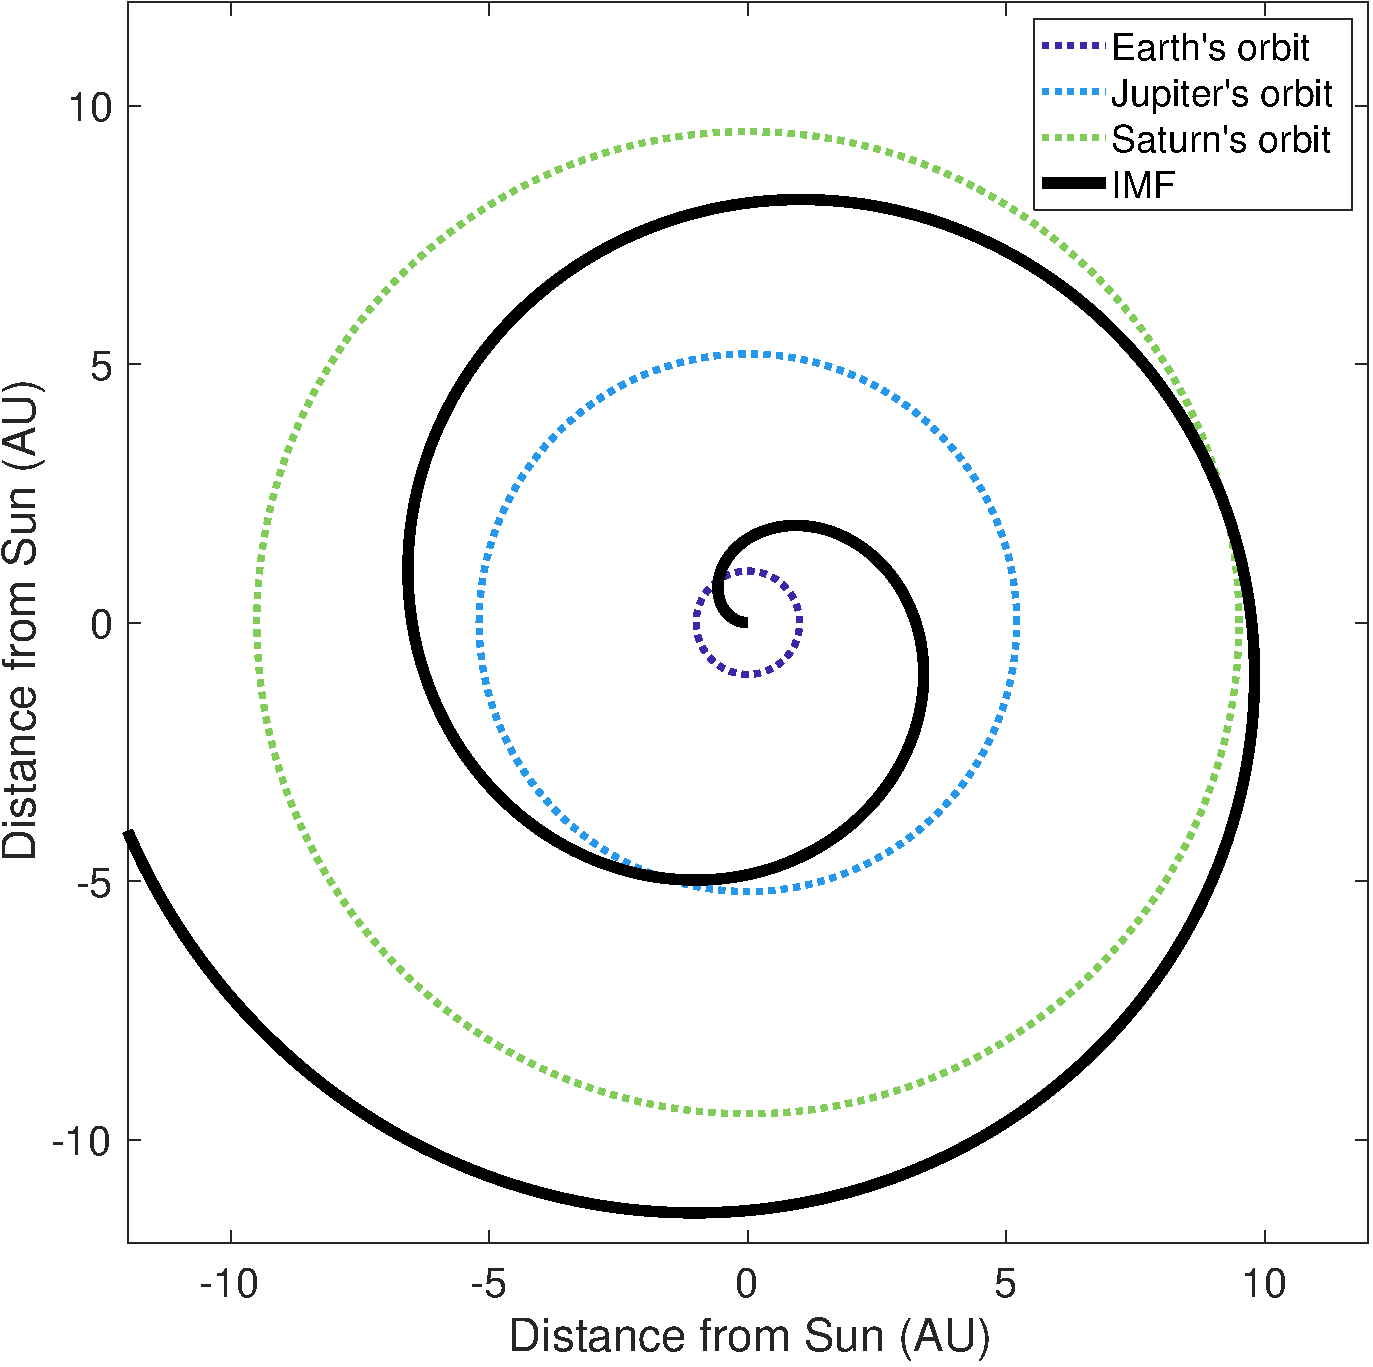
\includegraphics[width=0.6\textwidth]{intro/parkerspiral.pdf}
\caption[Diagram of the Parker Spiral throughout the solar system.]{Diagram showing how the Parker Spiral affects the orientation of the IMF (interplanetary magnetic field) in the equatorial plane throughout the solar system. The orbits of different planets are shown by the coloured dotted lines.}
\label{intro:fig:parkerspiral}
\end{figure}

On top of this rotating structure, the properties of the solar wind varies on timescales ranging from minutes to years. At the shorter end of the spectrum, coronal mass ejections (CMEs) are dynamic ejections of dense coronal material that occur due to reconfiguration of the coronal magnetic field. These typically form over days and may reach speeds as high as several thousand $\si{kms^{-1}}$ as they accelerate through the inner solar system. Their movements are associated with regions with enhanced densities and magnetic field strengths compared to the ambient solar wind \citep{odstrcil1999}. At the opposite end of the spectrum, it is well known that the Sun exhibits periodic behaviour with an approximately 11 year cycle, known as the solar cycle. This cycle of alternatively high and low solar activity can be tracked well by the number of sunspots that appear on the solar surface, and is correlated with solar wind properties such as solar irradiance, magnetic field strength, and flare and CME incidences \citep{hathaway2015}. There is therefore a great deal of variability in the magnetic and plasma environment of the solar system, over time and through space.

\section{Planetary Magnetospheres}
\subsection{Structure of a Magnetosphere}
A magnetosphere is a bubble of magnetised plasma that surrounds a planet with a significant internal magnetic field, and forms due to the interaction between this magnetic field and the solar wind. Mercury, Earth, and the outer giant planets all have approximately dipolar internal magnetic fields, generated by convective flow of electrically conducting fluid in the planets' deep interiors \citep{kivelson2014book}. Thus they all have stable magnetospheres.

The magnetopause is the surface that separates the internal planetary plasma of the magnetosphere from the external shocked solar wind plasma of the magnetosheath. The magnetosheath is the region between the magnetosphere proper and the bow shock, where the solar wind plasma is decelerated to subsonic speeds. In a steady state system, the shape and size of the magnetopause is determined by pressure balance across the boundary, between the internal magnetic and plasma pressures, and the external solar wind pressure. This in turn influences the configuration of the magnetosphere internally. Therefore, the structure of the magnetosphere varies significantly between different planets, where both the internal and external conditions are different. However, many features are broadly common to all planetary magnetospheres in some form, and Figure~\ref{intro:fig:magnetosphere} shows a diagram specifically of Earth's magnetosphere, with these main features labelled. Note that at Jupiter and Saturn, the internal planetary magnetic field is oppositely oriented such that the magnetic fields and current systems are all in the opposite direction.

\begin{figure}
\centering
\noindent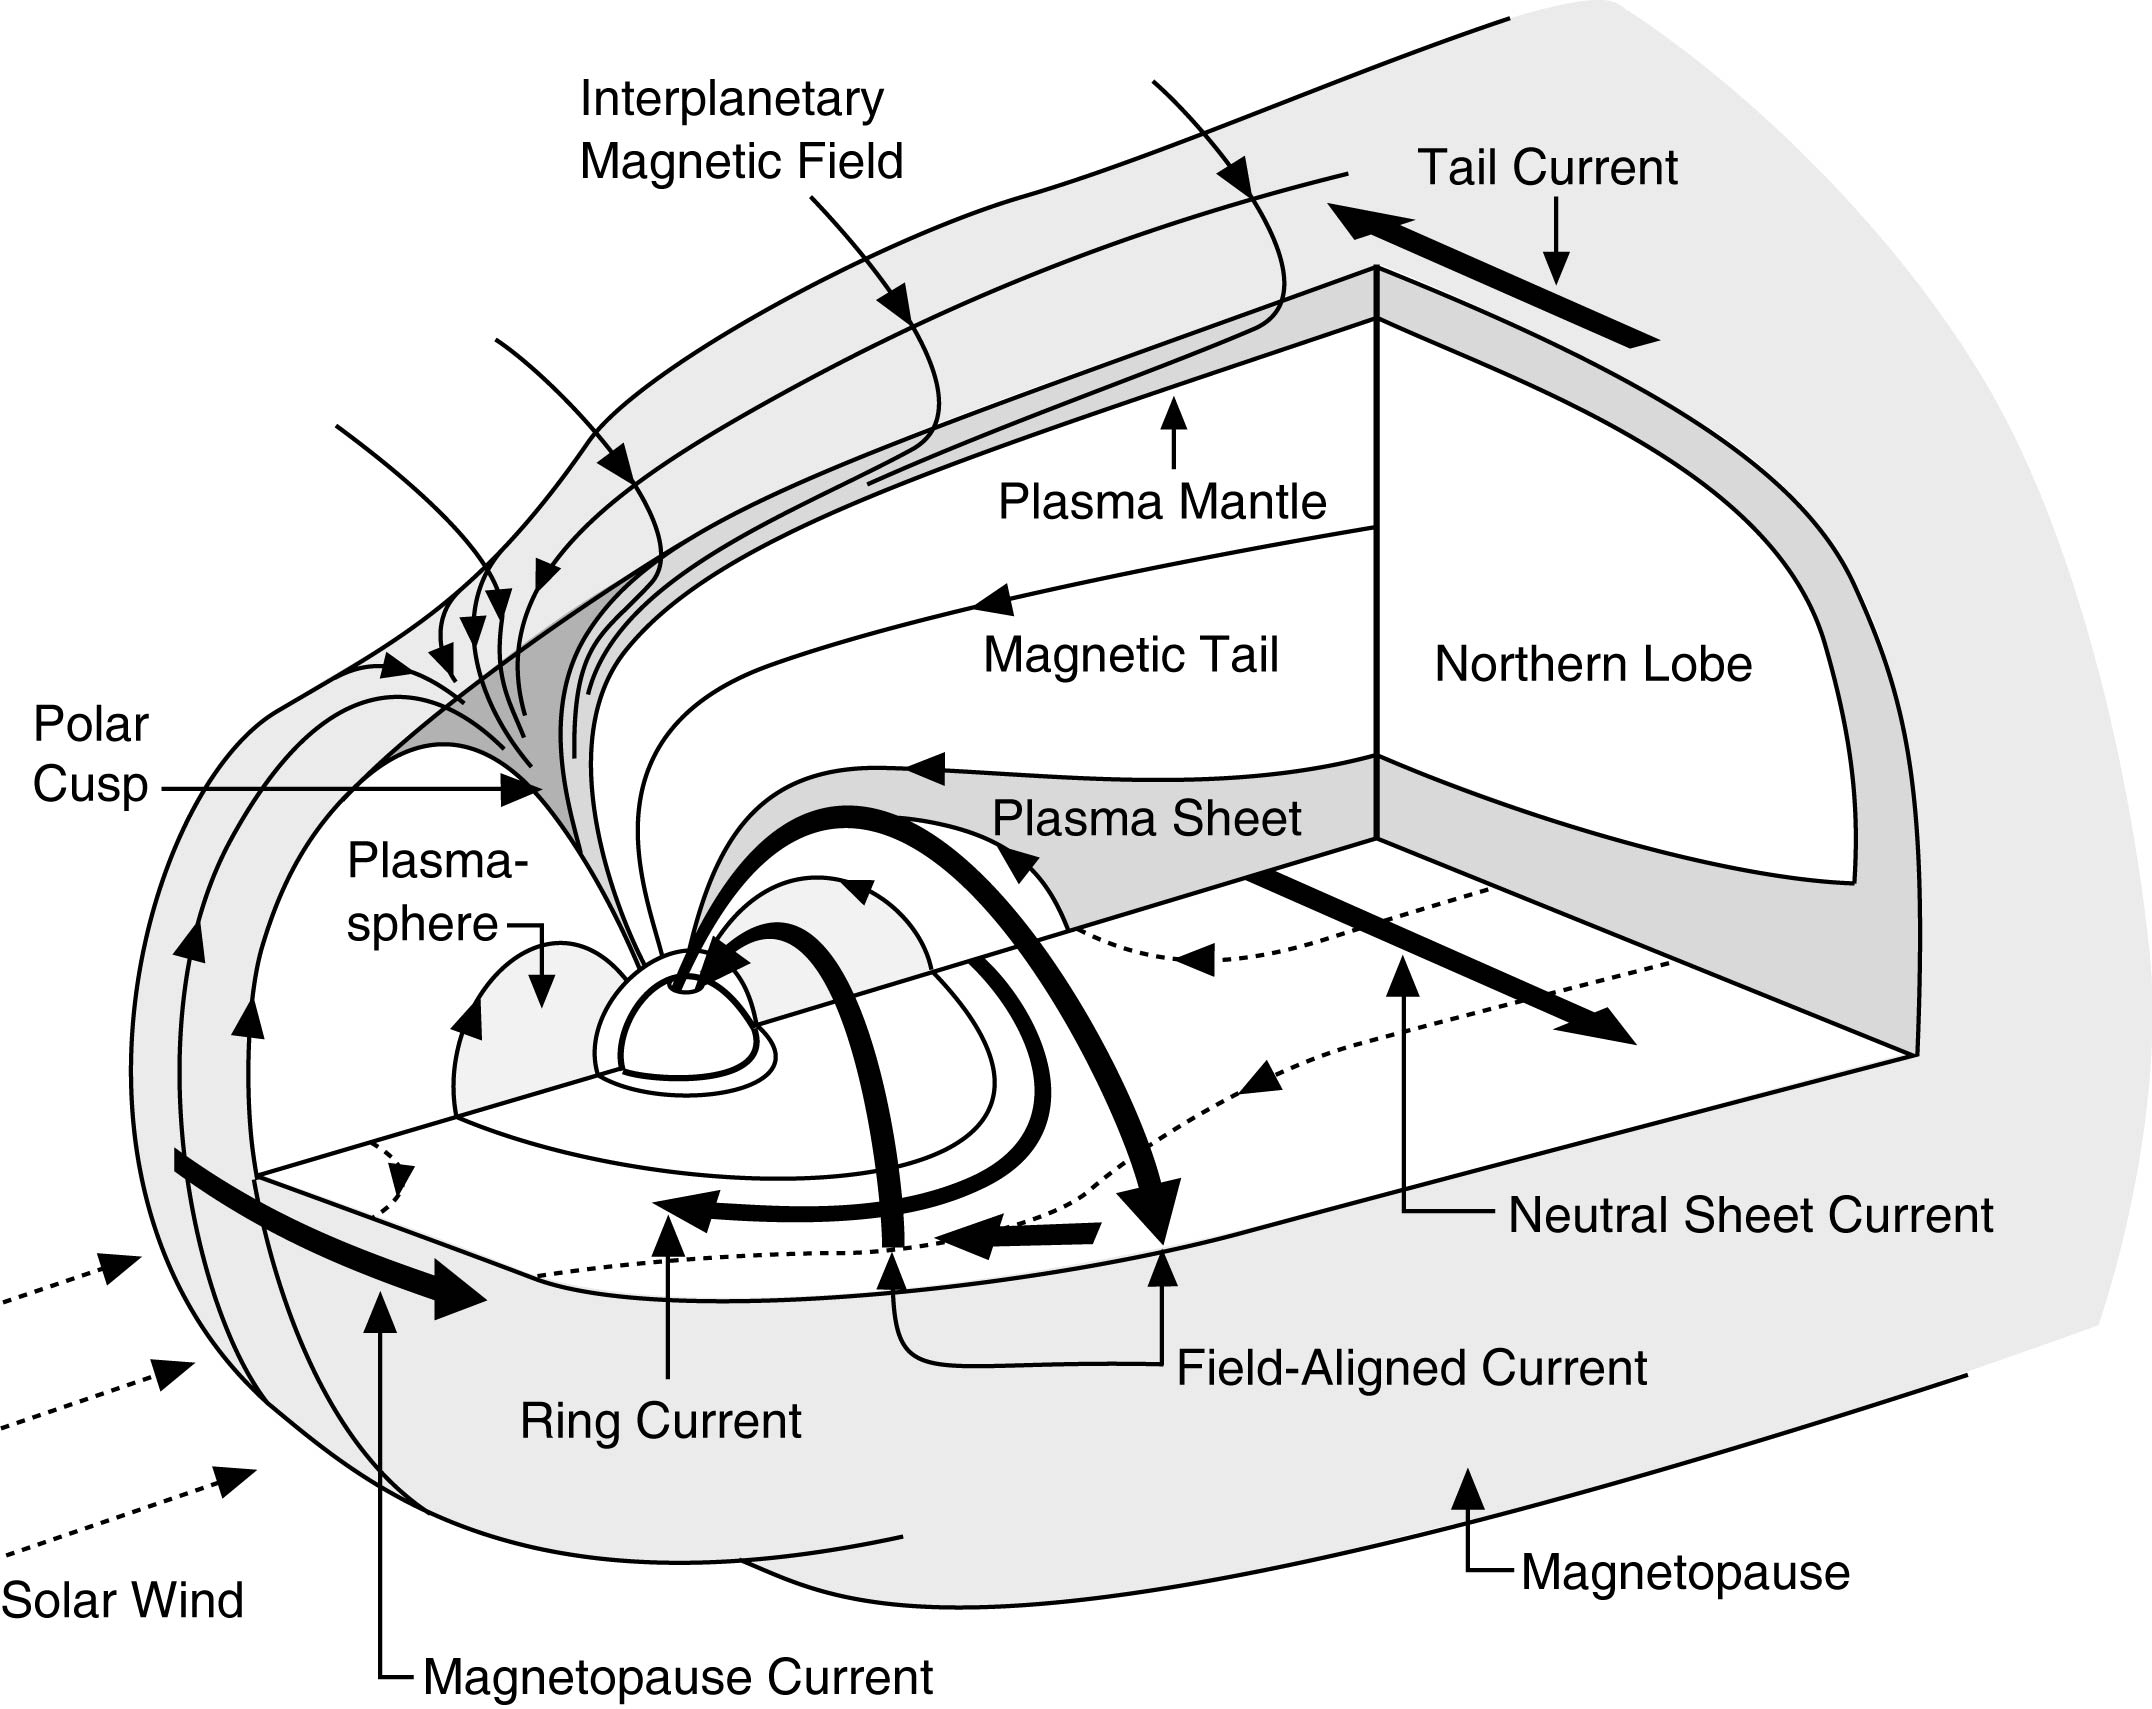
\includegraphics[width=0.8\textwidth]{intro/magnetospherediagram.jpg}
\caption[Diagram of Earth's magnetosphere.]{Diagram of the main features of Earth's magnetosphere from \citet{russell2016}, reproduced with permission.}
\label{intro:fig:magnetosphere}
\end{figure}

It can be seen that the magnetosphere is approximately dipolar in configuration on the dayside (i.e. the side facing the Sun), with a more extended `tail' on the nightside (i.e. the anti-sunward side), where the magnetic field lines stretch radially outwards and become approximately parallel to the solar wind direction. This tail can extend to tens or hundreds of planetary radii downstream of the planet; Jupiter's magnetotail has even been observed to extend as far as the orbit of Saturn, corresponding to several thousand Jovian radii downstream \citep{scarf1981}. Figure~\ref{intro:fig:magnetosphere} shows an azimuthal ring current system which orbits the planet near the equatorial plane; the direction is determined by the direction of the curvature and gradient drift velocities for positively charged particles in Earth's magnetic field, as described in Section~\ref{intro:sec:singleparticle} for the oppositely-oriented Saturn case. On the nightside this ring current extends into a current sheet, which separates the oppositely directed magnetic field lines in the northern and southern `lobes' of the magnetosphere. Currents also flow on the magnetopause and magnetotail surfaces as shown, separating the magnetic fields of the magnetosphere and the solar wind IMF. At the polar cusps, the magnetosphere is said to be `open' to the solar wind, as in these regions the internal planetary dipole magnetic field structure allows solar wind particles to access the magnetosphere. This is in contrast to the `closed' regions of the magnetosphere, where it is difficult for solar wind particles to penetrate.

\subsection{Comparative Magnetospheres}\label{intro:sec:comparativemagnetospheres}
A comparison of the magnetospheres of different planet systems is shown in Figure~\ref{intro:fig:magnetospherecomparison}. The most striking difference is in the overall size of the magnetospheres, and this is mainly due to the twin influences of the external solar wind conditions at each planet, and internal magnetic pressure associated with the planetary magnetic field. Table~\ref{intro:table:magnetospherecomparison} provides some typical parameters for the planets Earth, Jupiter and Saturn that help illustrate this. For example, the Jovian planetary dipole magnetic moment is some 20,000 times greater than that of Earth, with correspondingly higher magnetic field strength. This therefore means a much greater magnetic pressure inside Jupiter's magnetosphere. In addition, he solar wind dynamic pressure $D_\mathrm{P}$ is defined by 
\begin{equation}\label{intro:eq:dp}
D_\mathrm{P} = \rho_\mathrm{m}u^2
\end{equation}
where $\rho_\mathrm{m}$ is the mass density of the solar wind and $u_\mathrm{SW}$ is the velocity. As discussed in Section~\ref{intro:sec:solarwind}, $\rho_\mathrm{m}$ falls approximately as $r^{-2}$ while $u_\mathrm{SW}$ remains approximately constant, and so the external solar wind dynamic pressure is much lower for the planets in the outer solar system, falling as $r^{-2}$ .
\begin{figure}
\centering
\noindent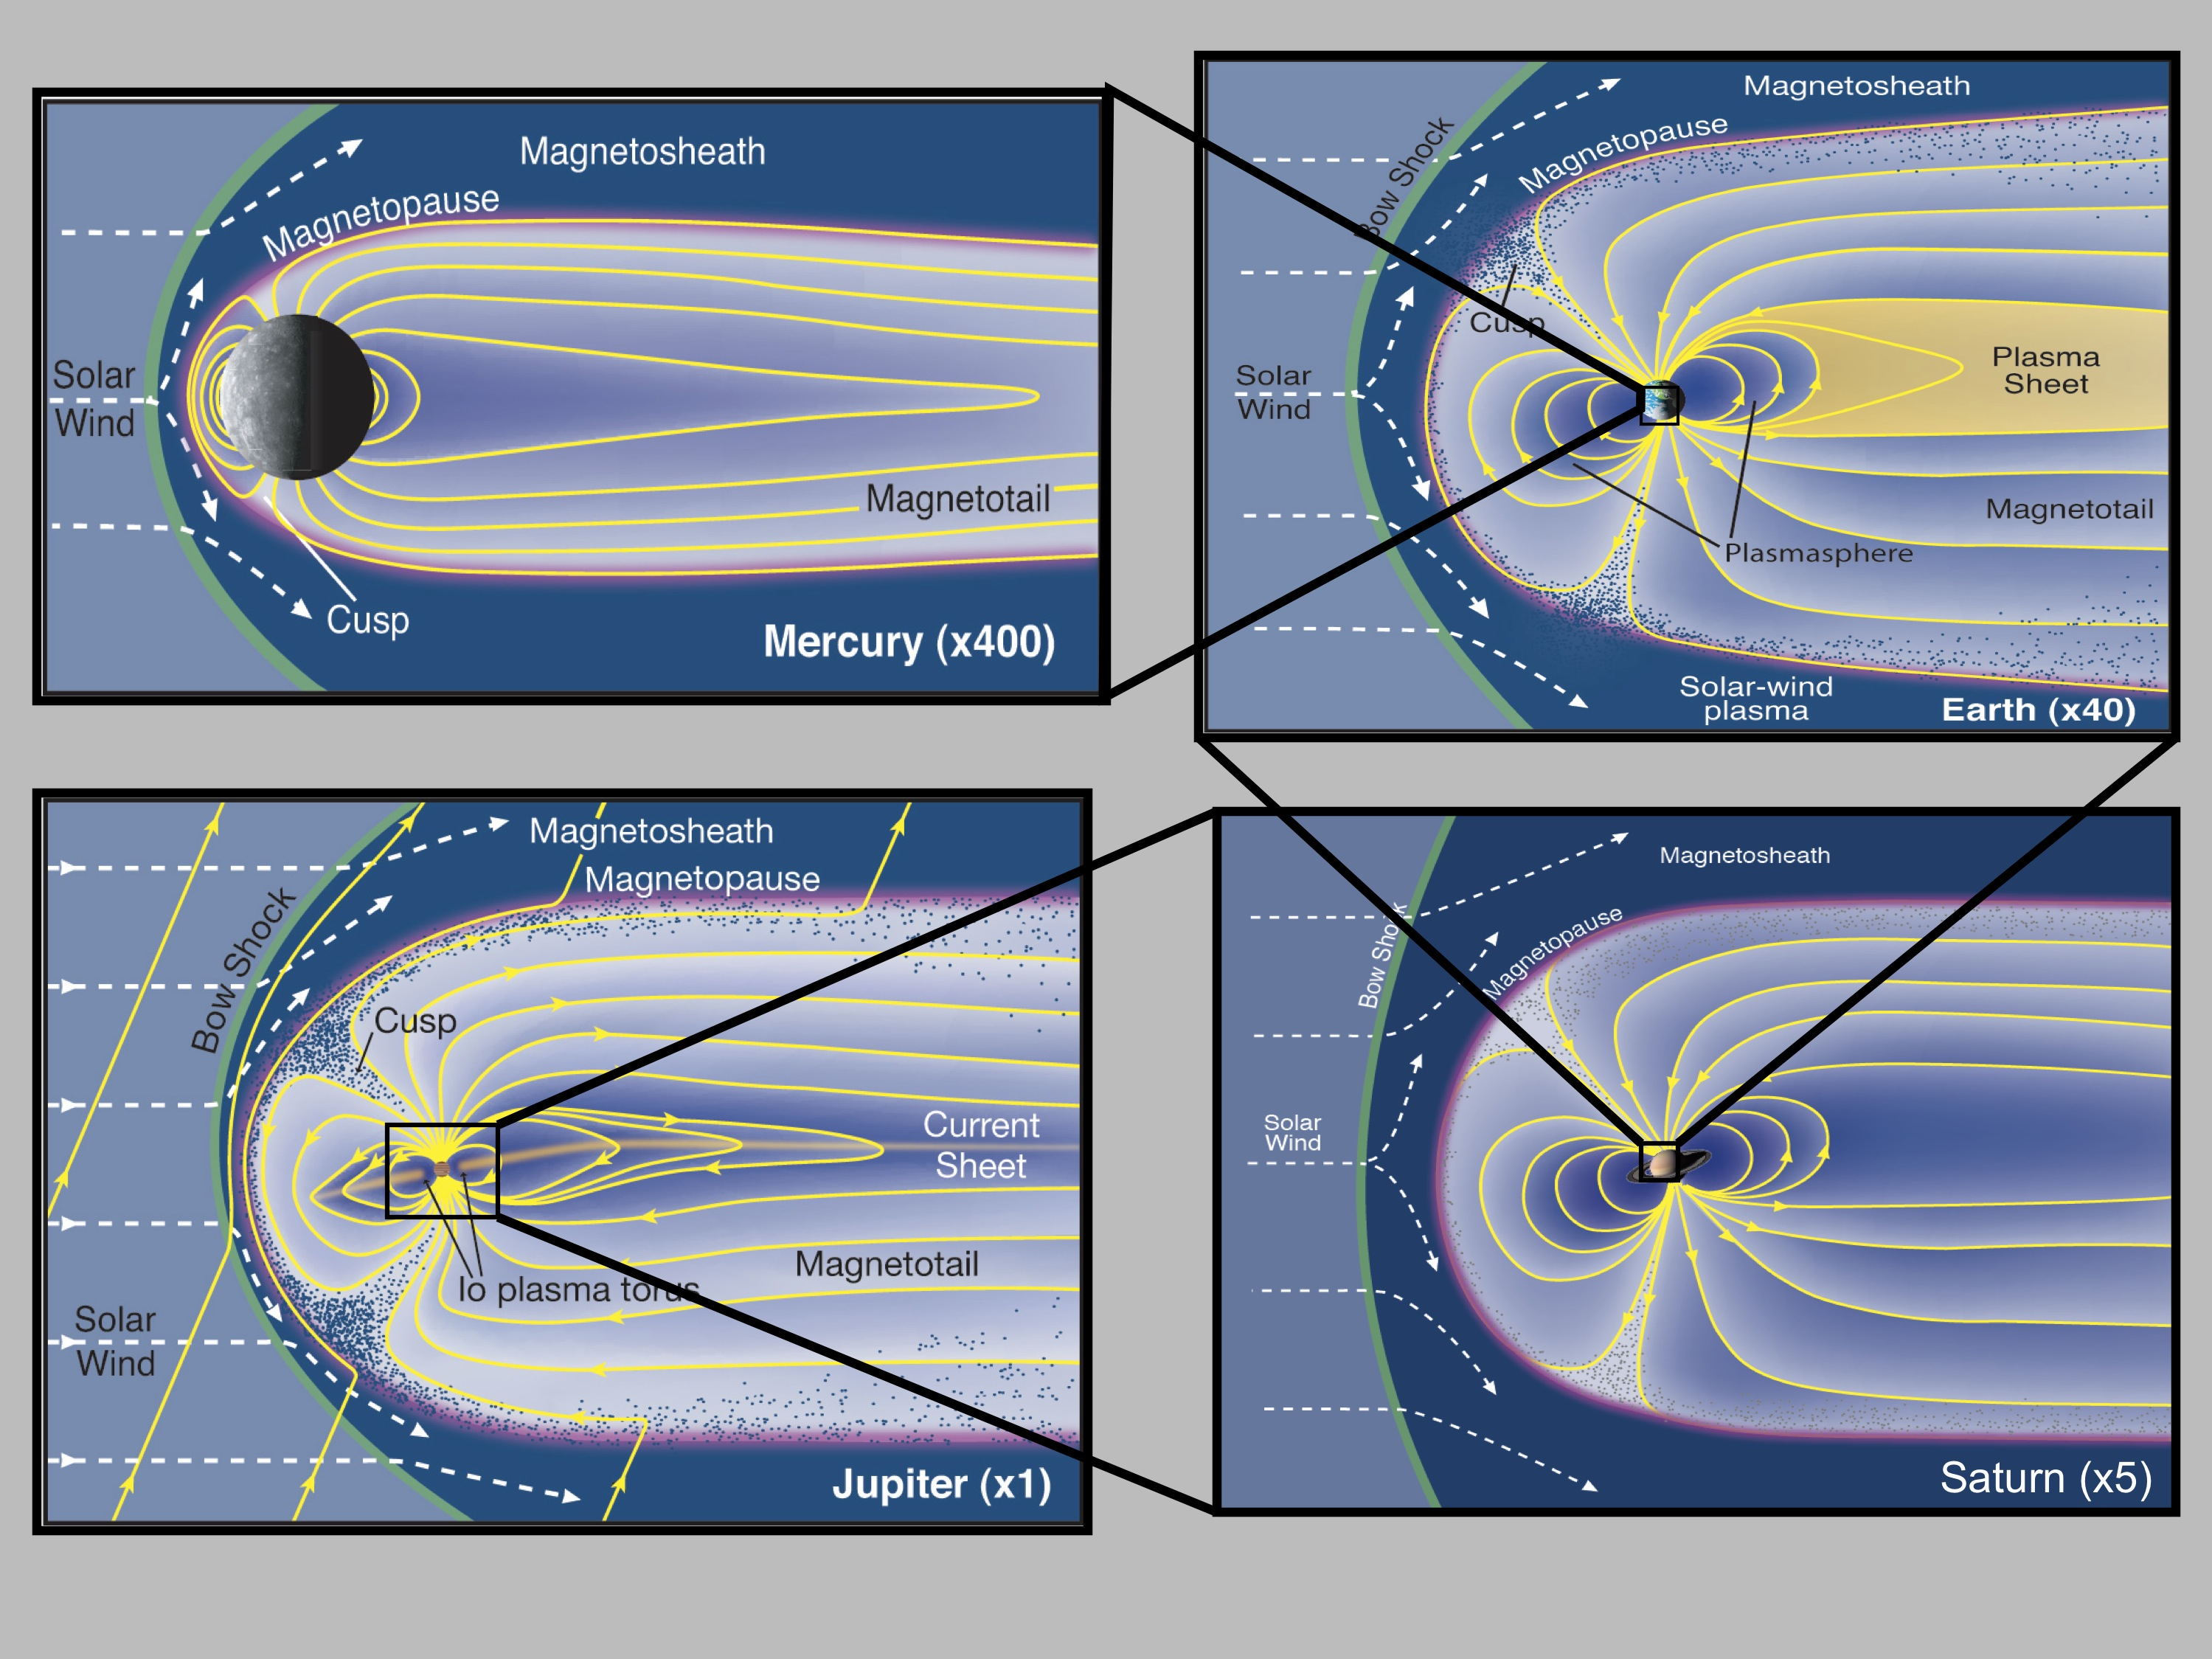
\includegraphics[width=1\textwidth]{intro/magnetospherecomparison.jpg}
\caption[Diagram of Mercury, Earth, Jupiter and Saturn magnetospheres.]{Diagram comparing the relative sizes and shapes of the magnetospheres of Mercury, Earth, Jupiter and Saturn, from Fran Bagenal and Steve Bartlett at LASP.}
\label{intro:fig:magnetospherecomparison}
\end{figure}
\begin{table}
\caption[Comparison of typical magnetospheric parameters for Earth, Jupiter and Saturn.]{Comparison of typical magnetospheric parameters for Earth, Jupiter and Saturn, adapted from \citet{bagenal2014} and references therein.}\label{intro:table:magnetospherecomparison}
\centering
\begin{tabular}{l c c c}
\hline
 																															& Earth						& Jupiter			& Saturn  \\
\hline
Planet radius $R_\mathrm{P}$ ($\si{km}$)															& 6,371					&	71,492			&	60,268 \\
Distance from Sun ($\si{AU}$)																			&	1							&	5.2				& 9.6		\\
Solar wind number density ($\si{cm^{-3}}$)														& 7							&	0.2				&	0.07		\\
Spin period ($\si{hr}$)																						&	24						& 	9.9				&10.6		\\
Magnetic moment ($\si{M_\mathrm{EARTH}}$)													&	1							&	20,000			&	600		\\
Equatorial surface magnetic field ($\si{nT}$)														&	30,600					&	430,000		&	21,400	\\
Dipole stand-off distance $R_\mathrm{CF}$	($\si{R_\mathrm{P}}$) 				&	$\SI{10}{R_\mathrm{E}}$ & $\SI{46}{R_\mathrm{J}}$ & $\SI{20}{R_\mathrm{S}}$ \\
Observed stand-off distance $R_\mathrm{MP}$ ($\si{R_\mathrm{P}}$)			&	$8-\SI{12}{R_\mathrm{E}}$ & $63-\SI{92}{R_\mathrm{J}}$ & $22-\SI{27}{R_\mathrm{S}}$ \\
\hline
\end{tabular}
\end{table}

This pressure-balance relationship is reflected in the `dipole stand-off distance' $R_\mathrm{CF}$ for each planet given in Table~\ref{intro:table:magnetospherecomparison}, where CF stands for Chapman-Ferraro as it was derived by \citet{chapman1930}. This distance is a theoretical location of the magnetopause, measured from the planet centre to the sub-solar point on the magnetopause surface, which would be expected if the external solar wind dynamic pressure was balanced exactly by the magnetic pressure associated only with an internal \textit{dipole} magnetic field. We can see that it is much greater for Jupiter and Saturn than for Earth, as expected from the pressure-balance explanation just given.

However at Saturn and Jupiter in particular, the observed magnetopause stand-off distances are significantly larger even than the Chapman-Ferraro estimates. This is mainly due to the significant internal plasma sources at each planet. At Saturn, the icy moon Enceladus orbits at a distance of $\SI{3.95}{R_\mathrm{S}}$, and ejects water group molecules into the magnetosphere at around \SI{150}{kg s^{-1}}, while at Jupiter, the volcanic moon Io orbits at $\SI{5.9}{R_\mathrm{J}}$ and ejects sulphur dioxide into the magnetosphere at around \SI{1000}{kg s^{-1}}~\citep{bagenal2011}. At each planet, this material is partially ionised, and the plasma pressure associated with this population adds to the internal magnetic pressure, inflating the magnetosphere beyond a dipolar internal field model. This is discussed in more detail in Section~\ref{intro:sec:pbalance}. In contrast at Earth, the Moon does not contribute a significant plasma population, and also mainly orbits the planet beyond the magnetosphere boundary, and so does not have the same influence on Earth's magnetosphere  \citep[e.g.][]{schneider1967}.

For Jupiter and Saturn, these internal plasma populations not only influence the overall size of the magnetosphere but also the internal structure of the magnetic field. This is due to the rapid rotation rates of the two planets, shown by the short spin periods in Table~\ref{intro:table:magnetospherecomparison}. Due to the aforementioned frozen-in field theorem, the magnetospheric plasma is azimuthally accelerated towards co-rotation with the rapidly rotating magnetic field of the magnetosphere. The centrifugal force associated with this confines the plasma towards the rotational equator, creating a thick plasma sheet. In order to balance this centrifugal force, the magnetic field is distorted around the plasma sheet from a dipolar magnetic field into a disc-like \textit{magnetodisc} structure, with a strong associated magnetic curvature force. This is characterised by field lines that are stretched radially outwards near the equatorial plane in outer magnetosphere, as can be seen particularly for Jupiter in Figure~\ref{intro:fig:magnetospherecomparison}, and is supported by the azimuthal ring current. The intensity of the ring current is enhanced by a population of hotter, more variable plasma that originates in the outer magnetosphere at both Saturn~\citep[e.g.][]{sergis2010} and Jupiter~\citep[e.g.][]{mauk2004}, with observed plasma $\beta$ of the order $2-5$ and ${\sim}100$ for these populations respectively. The magnetic field strength of this disk-like magnetic field structure in general varies more slowly with radial distance than a dipolar magnetic field, and thus also influences pressure balance at the magnetopause. This is investigated for both Saturn and Jupiter in Chapter~\ref{chap:compress}. 

\subsection{Magnetospheric Dynamics}\label{intro:sec:dynamics}
The simplest dynamical process that a magnetosphere undergoes is compression and expansion under varying solar wind conditions. For example, as the local solar wind dynamic pressure increases, due to an increase in velocity or number density by some process as described in Section~\ref{intro:sec:solarwind}, the magnetosphere is compressed. This compression causes the internal magnetic field pressure to increase, until it balances the enhanced external solar wind dynamic pressure and a new equilibrium magnetopause location is reached. If the solar wind pressure decreases, the magnetosphere then inflates. The magnetopause is therefore in constant motion, with a velocity or order $\SI{10}{kms^{-1}}$ at Earth \citep{berchem1982} and $\SI{100}{kms^{-1}}$ at Saturn \citep{masters2011}. The exact response of the magnetosphere to varying $D_\mathrm{P}$ varies significantly between planets due to the different internal structures. For Saturn in particular, the distance that the magnetopause location shifts for a given change in $D_\mathrm{P}$, and how this varies with different internal and external conditions, is the subject of the study in Chapter~\ref{chap:compress}, and is discussed in detail there.

However even under approximately constant solar wind conditions, a magnetosphere is not a static object. At the `solar-wind driven' magnetospheres Earth and Mercury, the dominant large-scale dynamic process is known as the \textit{Dungey Cycle}, after \citet{dungey1961}. A diagram of this process is shown in Figure~\ref{intro:fig:dungeycycle}. For an IMF oriented anti-parallel to the planetary magnetic field, conditions are favourable for reconnection of the two magnetic fields at the dayside magnetopause, as the magnetic field varies on small spatial scales (as discussed in Section~\ref{intro:sec:frozenin}). The planetary magnetic field lines are then open to the solar wind at one end whilst still anchored to the planet at the other, and are thus convected by the solar wind flow downstream to the nightside. This leads to a build-up of magnetic flux on field lines in the magnetotail, which then reconnect across the tail current sheet. This causes plasma to return on closed field lines back towards the planet on the nightside. At Earth, this process is associated with the generation of aurora along the boundary between open and closed magnetic field lines, in the northern and southern polar atmospheres \citep[e.g.][]{milan2007}. As the energetic electrons in the plasma gyrate around the polar magnetic field lines towards the planet, they excite atoms in the atmosphere, which then decay back to a lower energy level and emit photons in the process, which are observed as aurora.

\begin{figure}
\centering
\noindent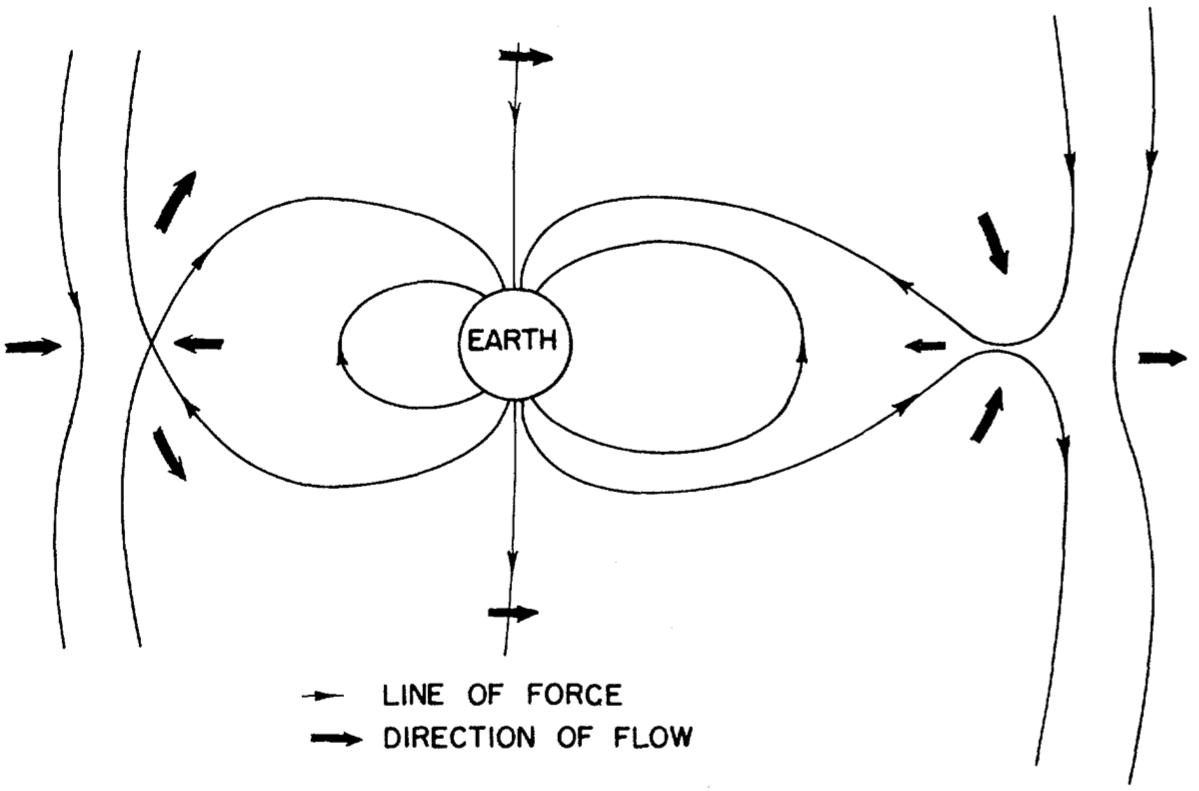
\includegraphics[width=0.8\textwidth]{intro/dungeycycle.png}
\caption[Diagram of the Dungey cycle.]{Diagram showing the Dungey Cycle process at Earth, from \citet{dungey1961}. Thin black `lines of force' are magnetic field lines. The solar wind flows from left to right.}
\label{intro:fig:dungeycycle}
\end{figure}

At Jupiter and Saturn, the dominant dynamical process is driven by the rapid planetary rotation, and thus we say they are `rotationally driven' magnetospheres. This process is known as the Vasyliunas cycle, after \citet{vasyliunas1983}, and a diagram depicting it is shown in Figure~\ref{intro:fig:vasyliunascycle}. As discussed in the previous section, these rapidly rotating magnetospheres have significant internal plasma populations, which are accelerated to near-corotation with the rotating planetary magnetic field. The centrifugal interchange instability causes this plasma to be transported radially outwards, such that inner cold, dense flux tubes are exchanged with outer hot, tenuous flux tubes \citep{southwood1989}, and the magnetic field is stretched out as shown in region 1 of Figure~\ref{intro:fig:vasyliunascycle}. As the flux tubes rotate around to the nightside, they are no longer as confined by the magnetopause boundary and so expand down the tail, and the magnetic field becomes increasingly more stretched (region 2) until reconnection occurs across the tail (region 3). This generates the release of a `plasmoid' down the tail, and the newly empty flux tube is then convected back around the planet on the dawn side. 

This cycle is dominant over the Dungey cycle for the outer giant planets due to the combined effects of the much faster rotation rates, and overall larger magnetospheric sizes, which means a much longer period of time for a magnetic field line to be convected across the polar cap from dayside to nightside \citep{forsyth2010}. However at Saturn in particular, it still uncertain how much of a role the Dungey cycle has to play \citep[e.g.][]{cowley2005}.

\begin{figure}
\centering
\noindent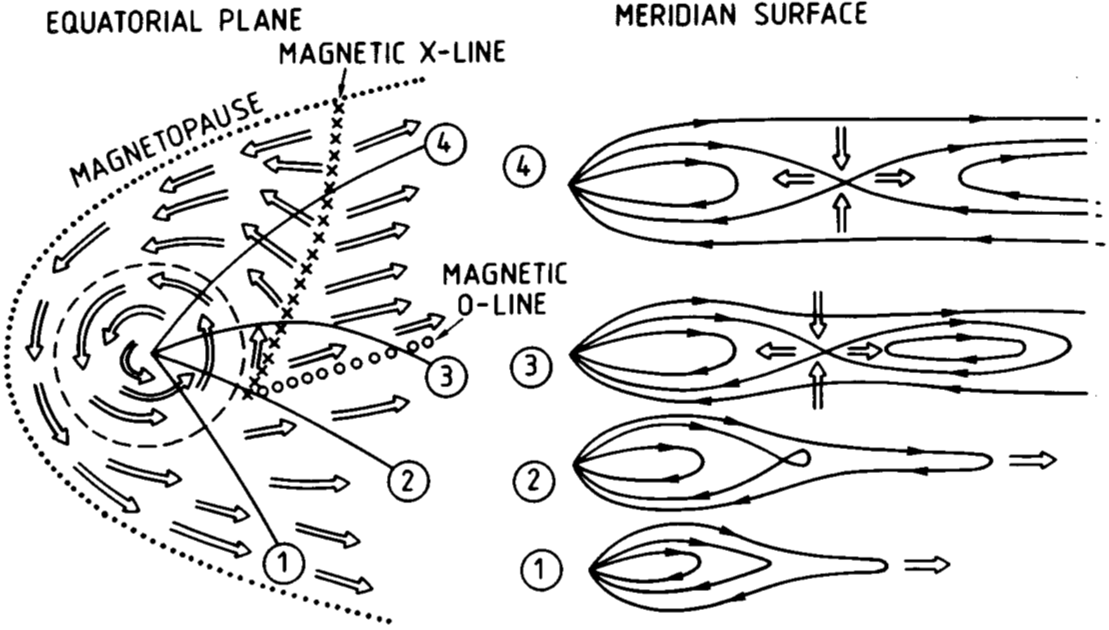
\includegraphics[width=0.9\textwidth]{intro/vasyliunascycle.png}
\caption[Diagram of the Vasyliunas cycle.]{Diagram showing the Vasyliunas cycle of plasma transport, from \citet{vasyliunas1983}. The dotted line shows the magnetopause boundary, the dashed line shows the region where plasma perfectly corotates with the magnetic field, and empty arrows show the plasma flow direction.}
\label{intro:fig:vasyliunascycle}
\end{figure}

In addition to these main modes of plasma transport in planetary magnetospheres, there are also numerous small-scale dynamical processes, such as Kelvin-Helmholtz vortices on the magnetopause surface; however these vary significantly between planets and are not relevant to the work of this thesis, and so we do not cover them explicitly here.

\section{Saturn and its Magnetosphere}\label{intro:sec:saturn}
%\subsection{Configuration of Saturn's Magnetosphere}
Saturn orbits the Sun once every ${\sim}29$ years, on an elliptical orbit at an average distance of \SI{9.6}{AU}. Saturn is approximately 10 times the size of Earth (by radius), and around 100 times as massive, meaning its density is around 1/10 Earth's. This is because Saturn is a `gas giant' planet, composed mainly of molecular hydrogen and helium, with a small rocky core. Between the core and the outer layers, the hydrogen is compressed to such high pressures and temperatures that it becomes `metallic', flowing and conducting electricity and generating the dynamo of Saturn's planetary magnetic field.

The internal planetary magnetic field is approximately dipolar, though with smaller higher order moments, and is offset northwards from the planetary equator by ${\sim}\SI{0.05}{R_S}$ \citep{dougherty2018}. Arguably the most interesting aspect of Saturn's internal magnetic field is that the dipole axis is extremely closely aligned with the planet spin axis, with the same study by \citet{dougherty2018} finding an upper limit of $\SI{0.01}{\degree}$ difference between them. This is seemingly in contradiction with Cowling's Theorem, which states that an active dynamo cannot maintain a perfectly axisymmetric magnetic field \citep{cowling1933}. This extreme axisymmetry also means it is near impossible to determine the rotation rate of the planet's deep interior; however, a range of periodic phenomena are observed at Saturn at periods assumed \textit{close} to the true planetary rotation rate, as discussed in detail in Section~\ref{intro:sec:periodicities}.

From Table~\ref{intro:table:magnetospherecomparison} and the associated discussion, we have seen that in many ways Saturn's magnetosphere is an intermediate between Earth and Jupiter. It is therefore a particularly interesting system to study, and can be used to learn more about magnetospheric physics in a global context. Saturn's magnetosphere was first investigated \textit{in situ} with single flybys by the outer solar system space missions \textit{Pioneer} (1979), \textit{Voyager I} (1980) and \textit{Voyager II} (1981). These observations did not reveal a significant magnetodisc magnetic field structure on Saturn's dayside (as was known to exist at Jupiter), although did provide some evidence for a thin current sheet on the dawn flank \citep{smith1980}. However with the arrival of the \textit{Cassini} space mission into orbit around Saturn in 2004, and its continued observation of the system until late 2017, our scientific understanding of Saturn's magnetosphere has been revolutionised. (The \textit{Cassini} space mission is discussed in detail in Chapter~\ref{chap:cassini}.)

We now know that in the outer magnetosphere, a non-negligible magnetodisc magnetic field structure exists at all local times beyond a radial distance of ${\sim}\SI{15}{R_S}$, due to the reasoning discussed in Section~\ref{intro:sec:comparativemagnetospheres}. However particularly on the dayside, it was found that a significant magnetodisc structure only forms under low solar wind dynamic pressure, where the subsolar magnetopause stand-off distance becomes greater than $\SI{23}{R_S}$, and that when it is more extremely compressed than this, the magnetic field remains approximately dipolar~\citep{arridge2008}. It is interesting that this value falls between the two modes of the bimodal distribution in magnetopause stand-off distances observed by \citet{pilkington2015}, of $\SI{20.7}{R_S}$ and $\SI{27.1}{R_S}$. This behaviour is broadly due to overall force balance in Saturn's magnetosphere; for a more expanded system, the magnetic field strength is weaker in the outer magnetosphere, and so a larger magnetic tension force is needed to balance the centrifugal and plasma pressure gradient forces acting radially outwards on the plasma. In Chapter~\ref{chap:compress} of this thesis, we present results that show the compressibility of the magnetosphere also changes behaviour at around this value of stand-off distance, at ${\sim}\SI{25}{R_S}$. 

The formation of a magnetodisc structure at Saturn is also influenced by the variable hot plasma population observed by \citet{sergis2010} and others, as discussed in Section~\ref{intro:sec:comparativemagnetospheres}, through an enhancement of the equatorial ring current intensity. By consideration of Amp\`ere's law, it can be understood that the magnetic field associated with an azimuthal current flowing in the direction of corotation decreases Saturn's planetary magnetic field in the inner magnetosphere, and increases it in the outer magnetosphere. This corresponds to a magnetodisc magnetic field structure. Many studies have attempted to characterise the thickness and radial extent of this equatorial ring current, using a combination of \textit{Cassini} data, and models such as that of \citet{connerney1981b, connerney1983}, which assumes an azimuthally symmetric current loop of uniform thickness. The nature of the ring current has been observed to vary significantly over time, with location, and with system size \citep[e.g.][]{bunce2007}, with a variable thickness of average ${\sim}\SI{3}{R_S}$ and significant radial extent, from around $\SI{7}{R_S}$ out to around $\SI{18}{R_S}$, at times reaching the magnetopause boundary on the dayside \citep[e.g.][]{kellett2009,sergis2009}. However due to incomplete coverage particularly across local time for most of the \textit{Cassini} mission, it was not until near the end of the mission that the local time asymmetry of the ring current was demonstrated by \citet{sergis2017}. Indeed, the local time variation in the large scale structure of Saturn's magnetosphere is still not fully understood, and is studied in this thesis in Chapter~\ref{chap:LTsectors} using a flexible model of the ring current adapted from \citet{achilleos2010a}.

\subsection{Planetary Period Periodicities}\label{intro:sec:periodicities}
%The equatorial current sheet is just one part of Saturn's magnetosphere that displays periodic dynamical behaviour, at a rate close to the planetary rotation rate. At Jupiter, the dipole axis is tilted relative to the rotation axis by $\SI{9.4}{\degree}$. The current sheet lies in the \textit{magnetic} equatorial plane, and so for a stationary observer, the current sheet appears to `flap' above and below the rotational equator once per planetary rotation. Similar behaviour is observed at Saturn, despite the aforementioned alignment oft the dipole and rotation axes, and hence must be caused by a more complicated process.
%Dynamic current sheet. A summary of periodicities, the history, the different values, when and where they were discovered and what they might mean.
Another key aspect of Saturn's magnetosphere that is still not fully understood, is the nature of the observed periodic variations in field and particle properties. These variations, summarised in \citet{carbary2013}, have periods ranging from around 10.6-10.8 hours, assumed close to the true planetary rotation rate. Magnetospheric periodicities include the location of the auroral oval \citep{provan2009b}, and the magnetopause boundary \citep{clarke2010}; the magnetic field strength and direction \citep{espinosa2000, andrews2008}; electron densities \citep{morooka2009}; ion distributions \citep{burch2009}; and energetic neutral atoms \citep{paranicas2005}. These observations are especially interesting due to the aforementioned axisymmetry of Saturn's magnetic field, which means they cannot be adequately explained by a geometric tilt of the magnetic field. In addition, some of the observed periods vary relatively quickly, by up to $1\%$ over the course of a year, and thus cannot be associated with changes to the planet's deep interior. This complex behaviour is apparently unique to Saturn, and has made it impossible to measure Saturn's true core rotation rate.

Initially, periodicities in radio observations of Saturn's auroral regions from the \textit{Voyager} spacecraft suggested a planetary rotation period of $\SI{10.657}{\hour}$ \citep{desch1981}. This radio emission is known as Saturn Kilometric Radiation, or SKR. However observations from the \textit{Ulysses} \citep{lecacheux1997} and later \textit{Cassini} \citep{gurnett2005} missions revealed that the SKR period was actually drifting over time, and thus could not be associated with the core rotation rate. A reanalysis of magnetometer data from the \textit{Voyager} and \textit{Pioneer} missions then showed a similar periodic behaviour in the magnetic field. This led to the development of a `camshaft' model, where a rotating equatorial magnetic anomaly that is fixed in longitude triggers radial waves that cause the observed perturbations \citep{espinosa2003b}. To further complicate the picture, two distinct periods were then discovered in the SKR signal by \textit{Cassini}, associated separately with the Northern and Southern hemispheres \citep{gurnett2009}. This phenomenon was then also observed in more recent \textit{Cassini} magnetic field observations \citep[e.g.][]{andrews2010,provan2012}. In these and other studies, such as \citet{hunt2014}, a picture has now been developed of how these hemispheric magnetic perturbations are generated, by two large-scale field-aligned current systems that rotate at slightly different rates in each hemisphere. The magnetic field associated with each current system is dominant in the respective hemisphere, and can be approximated in the outer magnetosphere by a rotating, transverse oriented dipole. However the true magnetic field perturbation is much more complex, and is currently an area of active research, with some final \textit{Cassini} results still to be fully analysed. The physical origins of these current systems are also still not fully understood, but are thought to be associated with twin atmospheric vortices flowing in the polar upper atmosphere/ionosphere in each hemisphere \citep{jiaandkivelson2012, southwood2014, smith2016}. 

In the equatorial plane, these magnetic field perturbations have the effect of making Saturn's current sheet appear to`flap' above and below the rotational equator once per planetary rotation \citep[e.g.][]{arridge2011}. Similar behaviour is also observed at Jupiter. However Jupiter the dipole axis is tilted \SI{9.4}{\degree} relative to its rotation axis, which means that relative to the rotational equator, the current sheet behaves approximately as a rotating, tilted disc, and so this behaviour is expected. In addition, at Saturn, these periodic magnetic field perturbations also have the effect of periodically thickening and thinning the current sheet at different longitudes \citep{provan2012}, associated with a large scale compression and expansion of the magnetosphere in a given region, known as `breathing' \citep{ramer2016}. Both the `flapping' and `breathing' behaviours are controlled by the relative phases of the northern and southern magnetic perturbations, noting that their independent rotation rates means the phase relationship between them changes over time. This complicated dynamical behaviour is the focus of much current research, and is the subject of the study in Chapter~\ref{chap:equinox}.

\subsection{Pressure Balance at the Magnetopause}\label{intro:sec:pbalance}
As previously mentioned, the magnetopause boundary can be approximated as the location where the effective pressure of the solar wind exerted on the magnetosphere is exactly balanced by the sum of the internal magnetospheric particle and field pressures. 

Before impacting on the magnetopause, the solar wind flow is first decelerated via the bow shock, and is deflected around the magnetosphere obstacle. This acts to reduce the dynamic pressure incident on the magnetopause surface, and must be accounted for when considering pressure balance. \citet{petrinec1997} used Bernoulli's equation in combination with the Rankine-Hugoniot jump conditions across the bow shock, assuming adiabatic flow of the solar wind, to show that the relation
\begin{equation}\label{intro:eq:pbalance1}
\frac{B_{\mathrm{MS}}^2}{2\mu_0} + P_{\mathrm{MS}} = kD_\mathrm{P}\cos^2\Psi + P_0\sin^2\Psi
\end{equation}
provides an approximation that is valid across the magnetopause surface, not just at the nose. For clarity the subscript {\sc{MS}} denotes magnetospheric properties, such that the terms on the left hand side of equation \ref{intro:eq:pbalance1} are the magnetospheric magnetic and plasma pressures respectively. $\Psi$ is the flaring angle measured between the upstream flow velocity vector and the normal to the magnetopause surface, such that $\Psi=0$ at the nose and generally increases as you move anti-sunward along the magnetopause surface. The first term on the right hand side is associated with the solar wind dynamic pressure, where $k$ is a positive constant $\leq1$ to account for the aforementioned diversion of flow, and the $\cos^2\Psi$ factor accounts for the reduction in the normal component of dynamic pressure on the flanks and tail of the magnetosphere. The second term on the right hand side is composed of a `static' pressure $P_0$ associated with the thermal pressure of the solar wind, and a $\sin^2\Psi$ factor to ensure a real (i.e. not imaginary) flow velocity in the subsolar region \citep[see][]{petrinec1997}.

In order to improve agreement with the results of MHD simulations from \citet{hansen2005}, and to improve the consistency of $D_\mathrm{P}$ estimates, \citet{kanani2010} proposed a modification to this relation such that $P_0$ is dependent on $D_\mathrm{P}$. The relationship then becomes

\begin{equation}\label{intro:eq:pbalance2}
\frac{B_\mathrm{MS}^2}{2\mu_0} + P_\mathrm{MS} = [k\cos^2(\Psi) + \frac{k_\mathrm{B}T_\mathrm{SW}}{1.16m_\mathrm{p}u_\mathrm{SW}^2}\sin^2(\Psi)] D_\mathrm{P}
\end{equation}

where $k_\mathrm{B}$ is the Boltzmann constant, $m_\mathrm{p}$ is the mass of a proton, and $T_\mathrm{SW}$ and $u_\mathrm{SW}$ are the solar wind temperature and velocity respectively. The value of $k$ depends on the ratio of specific heats $\gamma$ in the solar wind, and the upstream sonic Mach number $M$. For high (${\gtrsim}8$) Mach number flow with $\gamma = 5/3$, $k = 0.881$ \citep{spreiter1966}, which is a valid assumption for the solar wind at Saturn's orbit \cite[e.g.][]{slavin1985,achilleos2006}.

This relationship allows an approximation of the solar wind dynamic pressure to be made, when only internal information about the state of the magnetosphere is known. 
Thus this relation is often used in studies that attempt to model the shape and size of the magnetopause boundary in response to changing $D_\mathrm{P}$, using only \textit{in situ} \textit{Cassini} data about the magnetic and plasma pressure inside the magnetosphere. These studies are discussed in more detail in Chapter~\ref{chap:compress}.

\section{A Force-Balance Model of Saturn's Magnetodisc}\label{intro:sec:forcebalancemodel}
Throughout this thesis we will employ the magnetodisc model from \citet{achilleos2010a}, with appropriate modifications as described in each chapter. This model is based on a magnetic field and plasma model originally constructed for the Jovian magnetodisc by \citet{caudal1986}, and adapted for the Saturn system. More information can be found in \citet{achilleos2010a, achilleos2010b}. The model is axisymmetric about the planetary dipole/rotation axis, which are assumed to be parallel. It is constructed based on the assumption of force balance in the rotating plasma of the magnetosphere between the Lorentz body force (including magnetic pressure and tension forces), pressure gradient force and centrifugal force, such that 
\begin{equation}\label{intro:eq:forcebalance}
\boldsymbol{J} \times \boldsymbol{B} = \nabla P - nm_i\omega^2\rho\boldsymbol{e}_\rho
\end{equation}
where $\rho$ is cylindrical radial distance from the axis, with $\boldsymbol{e}_\rho$ its unit vector. The plasma properties are isotropic pressure $P$, temperature $T$, ion number density $n$, mean ion mass $m_i$ and angular velocity $\omega$. Note that this construction is equivalent to equation~\ref{intro:eq:momentum}, the MHD momentum equation, with simplifying assumptions as described in that section, assuming force balance such that the acceleration of the plasma is zero, and including the centrifugal force on the plasma associated with the planetary rotation.

Any magnetic field can be presented in terms of two Euler potentials $\alpha$ and $\beta$, such that 
\begin{equation}
\boldsymbol{B} = \nabla \alpha \times \nabla \beta.
\end{equation}
(Note this has no relation to the plasma $\beta$, ratio of plasma to magnetic pressure.) For an axisymmetric field with no azimuthal component, the forms of $\alpha$ and $\beta$ can be chosen such that the magnetic field configuration is fully defined by one Euler potential which we call $\alpha = \alpha(r,\mu)$, where $r$ is radial distance from the origin, and $\mu = \cos\theta$, the cosine of colatitude. Using this form of $\alpha$, \citet{caudal1986} demonstrated that equation~\ref{intro:eq:forcebalance} is equivalent to the partial differential equation
\begin{equation}\label{intro:eq:pde}
\frac{\partial^2\alpha}{\partial r^2} + \frac{1-\mu^2}{r^2} \frac{\partial^2\alpha}{\partial \mu^2} = -g(r,\mu,\alpha)
\end{equation}
where $g(r,\mu,\alpha)$ is a source function determined by the distribution of plasma and angular velocity in $r,\mu$ space. This equation can be solved semi-analytically using Jacobi polynomials as laid out in detail in \citet[Appendix]{achilleos2010a} to give surfaces of constant $\alpha$, corresponding to magnetic field lines, in $r, \mu$ space. The model solution also provides a prediction of the local plasma pressure, and the azimuthal current density components associated with each of the terms on the right hand side of equation \ref{intro:eq:forcebalance}. 

Since the source function is itself dependent on $\alpha$, equation \ref{intro:eq:pde} must be solved iteratively, starting from a pure dipole magnetic field and then successively perturbing it. At each iteration, a linear combination of the present solution $\alpha_i$ and the previous solution $\alpha_{i-1}$ is used as input for the next iteration calculation, such that
\begin{equation}
\alpha_{i+1\mathrm{(input)}} = \gamma\alpha_i + (1-\gamma)\alpha_{i-1},
\end{equation}
where $\gamma<1$ controls the relative weighting between the previous and current solutions. This is a form of numerical relaxation. This $\alpha_{i+1(\mathrm{input})}$ is then used to calculate the source function in equation~\ref{intro:eq:pde} to solve for $\alpha_{i+1}$. In the original model construction, the two components were weighted equally ($\gamma=0.5$) and calculations continued until the maximum difference between successive iterations fell below a chosen `tolerance' $\delta = 0.5\%$, considered as convergence. In some of the work in this thesis we found that, for models with more extreme input parameters, it was necessary to weight the previous solution up to four times more heavily than the present solution ($\gamma=0.2$), in order to achieve convergence. (Exactly what constitutes an `extreme parameter' will be discussed in future chapters.) In order to keep the ratio $\delta/\gamma$ constant at $10^{-2}$, and therefore consistent with the original model approach, this corresponds to using a more stringent stopping tolerance $\delta = 10^{-2}\times0.2 = 0.2\%$ in such cases.

The global plasma properties can then be inferred entirely from the calculated magnetic field structure, using appropriate boundary conditions, as follows. \citet{caudal1986} explained that as a consequence of equation~\ref{intro:eq:forcebalance}, with $T$ and $\omega$ constant along magnetic field lines (according to Liouville's theorem and Ferraro's isorotation theorem respectively), the plasma pressure P is determined by 
\begin{equation}\label{intro:eq:p}
P = P_{0}\exp\left(\frac{\rho^2-\rho_0^2}{2\ell^2}\right),
\end{equation}
where $\ell$ is the \textit{confinement scalelength} (in $\rho$)
\begin{equation}
\ell^2 = \frac{2k_BT}{m_i\omega^2}.
\end{equation}
The subscript 0 means the quantity evaluated at the equatorial crossing point of the magnetic field line. This represents the plasma being confined towards the rotational equatorial plane due to the centrifugal force exerted on it. The model assumes that the plasma is composed of a cold and hot population; for the hot plasma population, the thermal energy associated with the plasma is significantly greater than the centrifugal potential, and so $\ell^2$ tends to infinity, such that the hot plasma pressure is not confined to the equator but is constant along magnetic field lines, $P_\mathrm{H} = P_\mathrm{H0}$. This is supported by observations made using data from \textit{Cassini} MIMI, such as \citet{krimigis2007}. Hence, the full form of equation~\ref{intro:eq:p} is only necessary for calculating the cold plasma pressure.

The requisite boundary conditions for the model are, then, the equatorial radial profiles of plasma properties. These were obtained from studies using results mainly from \textit{Cassini} plasma instruments CAPS and MIMI/INCA, as summarized in \citet{achilleos2010a}, and updated in \citet{achilleos2010b}. For the cold plasma population, the profiles for $m_i$ and $T$ were obtained from \citet{wilson2008}, $\omega$ profiles from \citet{wilson2008} and \citet{kane2008}, and the flux tube content information from \citet{mcandrews2009}. For the studies described in Chapters \ref{chap:equinox} and \ref{chap:LTsectors} we updated some of these boundary conditions using more recent results from \citet{wilson2017}, as described in those chapters.

As the hot plasma pressure is assumed uniform along magnetic field lines, the plasma population may be completely characterised by a particular equatorial plasma pressure $P_\mathrm{H0}$ and flux tube volume $V$ per unit of magnetic flux, where
\begin{equation}\label{intro:eq:ftv}
V = \int_{0}^{s_{B}} ds/B,
\end{equation}
and $ds$ is an element of arc length along the magnetic field line. The integral limits represent measurement along a field line of total length $s_B$ between the southern and northern ionospheric footprints at $\SI{1}{R_S}$. The flux tube volume is therefore dependent on both the shape of magnetic field lines, via $ds$, and the strength of the field, via $B$. Studies using \textit{Cassini} MIMI data such as \citet{sergis2007} found that the equatorial pressure associated with the hot plasma population was highly variable with $\rho$ and over time, as described in Section~\ref{intro:sec:saturn}. In light of these observations, the original \citet{achilleos2010a} model simply parameterised the global hot plasma content by a single `hot plasma index' $K_\mathrm{H}$, where $ K_\mathrm{H}= P_\mathrm{H0}V$ is constant beyond $\SI{8}{R_S}$, and $P_\mathrm{H0}$ decreases linearly to 0 inside that distance. A similar parameterisation, though with different values of the constants, was made in \citet{caudal1986}, who argued that for the Jovian system, under the expected conditions of rapid radial diffusion, the hot plasma would be transported isothermally. In \citet{achilleos2010a} the authors used a value of $K_\mathrm{H} = \SI{2e6}{Pa m T^{-1}}$ to represent `typical' hot plasma content conditions at Saturn, although results presented in that study suggest $K_\mathrm{H}$ may vary in the range $10^5{\--}10^7~\si{Pa m T^{-1}}$. Parameterising the hot plasma content in this way provides the flexibility to very simply characterize the level of ring current activity in the model, and thus investigate the effect of the varying hot plasma content on magnetospheric structure, and magnetospheric compressibility. This is the basis of the study described in Chapter~\ref{chap:compress}. In Chapter~\ref{chap:LTsectors}, this hot plasma pressure boundary condition is updated to describe different local time sectors, using recent results from \citet{sergis2017}.

Finally, at every iteration, a small uniform southward-directed `shielding field' is added to the magnetic field, in order to approximately account for the magnetic field associated with the magnetopause and magnetotail current sheets. Sketches of these current systems are included in the diagram in Figure~\ref{intro:fig:magnetosphere}, though note they are in the opposite sense for the Saturn system due to the opposite orientation of Saturn's planetary dipole. In \citet{achilleos2010a} the magnitude of this field was chosen by calculating dayside equatorial averages of the empirical field models of \citet{alexeev2005} and \citet{alexeev2006}, and it varied with model magnetodisc radius $R_\mathrm{D}$ \citep[see][Figure 6]{achilleos2010a}. In particular the component of the shielding field associated with the magnetopause currents was based on a dipole approximation of the magnetospheric magnetic field. In Chapter~\ref{chap:equinox} we update this calculation for a more realistic magnetodisc magnetic field, and in Chapter~\ref{chap:LTsectors} we modify this calculation using local time sector averages of the models of \citet{alexeev2005} and \citet{alexeev2006}, to account for the increased significance of the tail current field compared to the magnetopause current field for nightside local time sectors.

\section[Open Questions about Saturn's Magnetosphere]{Open Questions about Saturn's Magnetosphere: Motivations and Summary of this Thesis}
As a community, we are still trying to understand the large-scale structure of Saturn's magnetosphere, and how it varies in response to internal and external influences. We know that the rapid planetary rotation rate, significant internal hot and cold plasma populations, and external solar wind conditions all play a role in determining the configuration of the magnetosphere – but which factor is dominant, and does this relationship change under different conditions and in different places?

The answers to these questions have consequences for other areas of magnetospheric physics at Saturn. In Sections~\ref{intro:sec:comparativemagnetospheres} and \ref{intro:sec:pbalance} we touched on the concept of magnetospheric compressibility, and how the size of the magnetosphere scales with varying solar wind dynamic pressure. From equation~\ref{intro:eq:pbalance2}, it can be seen that the relative magnitudes of the magnetic and plasma pressures just inside the magnetopause are important in determining this pressure balance, and hence the system size. Therefore an investigation of the magnetospheric compressibility, and how it varies under different conditions, can reveal information about overall pressure balance within the magnetosphere. In Chapter~\ref{chap:compress} we investigate this compressibility using the \citet{achilleos2010a} magnetodisc model calculated at different system sizes. This approach complements previous observational studies based on \textit{Cassini} data, and also provides an opportunity to explicitly investigate the influence of the variable hot plasma population on the compressibility behaviour. We also use our results to make a direct comparison with the compressibility of Jupiter's magnetosphere, to test our expectations that Saturn behaves as an intermediate between Earth and Jupiter.

The structure of Saturn's magnetodisc, and in particular the equatorial current sheet, also has consequences for understanding the periodic perturbations in Saturn's magnetic field. We discussed in Section~\ref{intro:sec:periodicities} how Saturn's current sheet is observed to both `flap' and `breathe' periodically, at approximately the planetary rotation rate, due to rotating hemispheric magnetic perturbations. However this complicated behaviour is still not fully understood, and research is ongoing in the community using both \textit{Cassini} data analysis and MHD modelling approaches. In Chapter~\ref{chap:equinox} we attempt to model these two periodic behaviours simultaneously, using the \citet{achilleos2010a} magnetodisc model at different sizes to characterise the configuration of the magnetodisc at different phases of the planetary rotation. This allows us to provide an insight into how the breathing behaviour manifests in the \textit{Cassini} magnetic field observations, and utilises the knowledge gained in the previous chapter of this thesis, about how magnetospheric structure varies with system size. In addition for the flapping motion, we use a geometric model of a tilted and rippled current sheet and fit the combined model to \textit{Cassini} magnetic field observations, to investigate how the behaviour varies over time and under different conditions.

We still do not have a complete picture of how the large-scale structure of Saturn's magnetosphere varies across magnetic local time. In particular the dawn/dusk asymmetry in the magnetic field configuration is not well constrained. This is in part due to historically poor sampling of the dawn sector for much of the \textit{Cassini} space mission, and the generally smaller scale asymmetries between the two sectors compared to noon/night, although recent results from MHD simulations have provided some insights. It is important to investigate local time asymmetry in the magnetospheric magnetic field structure as this has consequences for other magnetic phenomena at Saturn, such as the location of the main auroral oval, and the aforementioned periodic modulation in the current sheet thickness. Therefore in Chapter~\ref{chap:LTsectors} we investigate this local time variation using a version of the \citet{achilleos2010a} model to characterise four different local time sectors, using more recent \textit{Cassini} observations as boundary conditions to improve our characterisation of local times beyond noon.

Finally, in Chapter~\ref{chap:conclusions} we summarise the key results of the work presented in this thesis, and suggest avenues for future research that can best utilise these results, in order to continue our pursuit of understanding the configuration of Saturn's magnetosphere.

But first, we must discuss in more depth the other tool we use to investigate Saturn's magnetosphere; the \textit{Cassini} space mission to Saturn.
\chapter{The Cassini-Huygens Mission}
\label{chap:cassini}
\section{Overview}
%http://sci.esa.int/cassini-huygens/33415-summary/
\begin{figure}
\centering
\noindent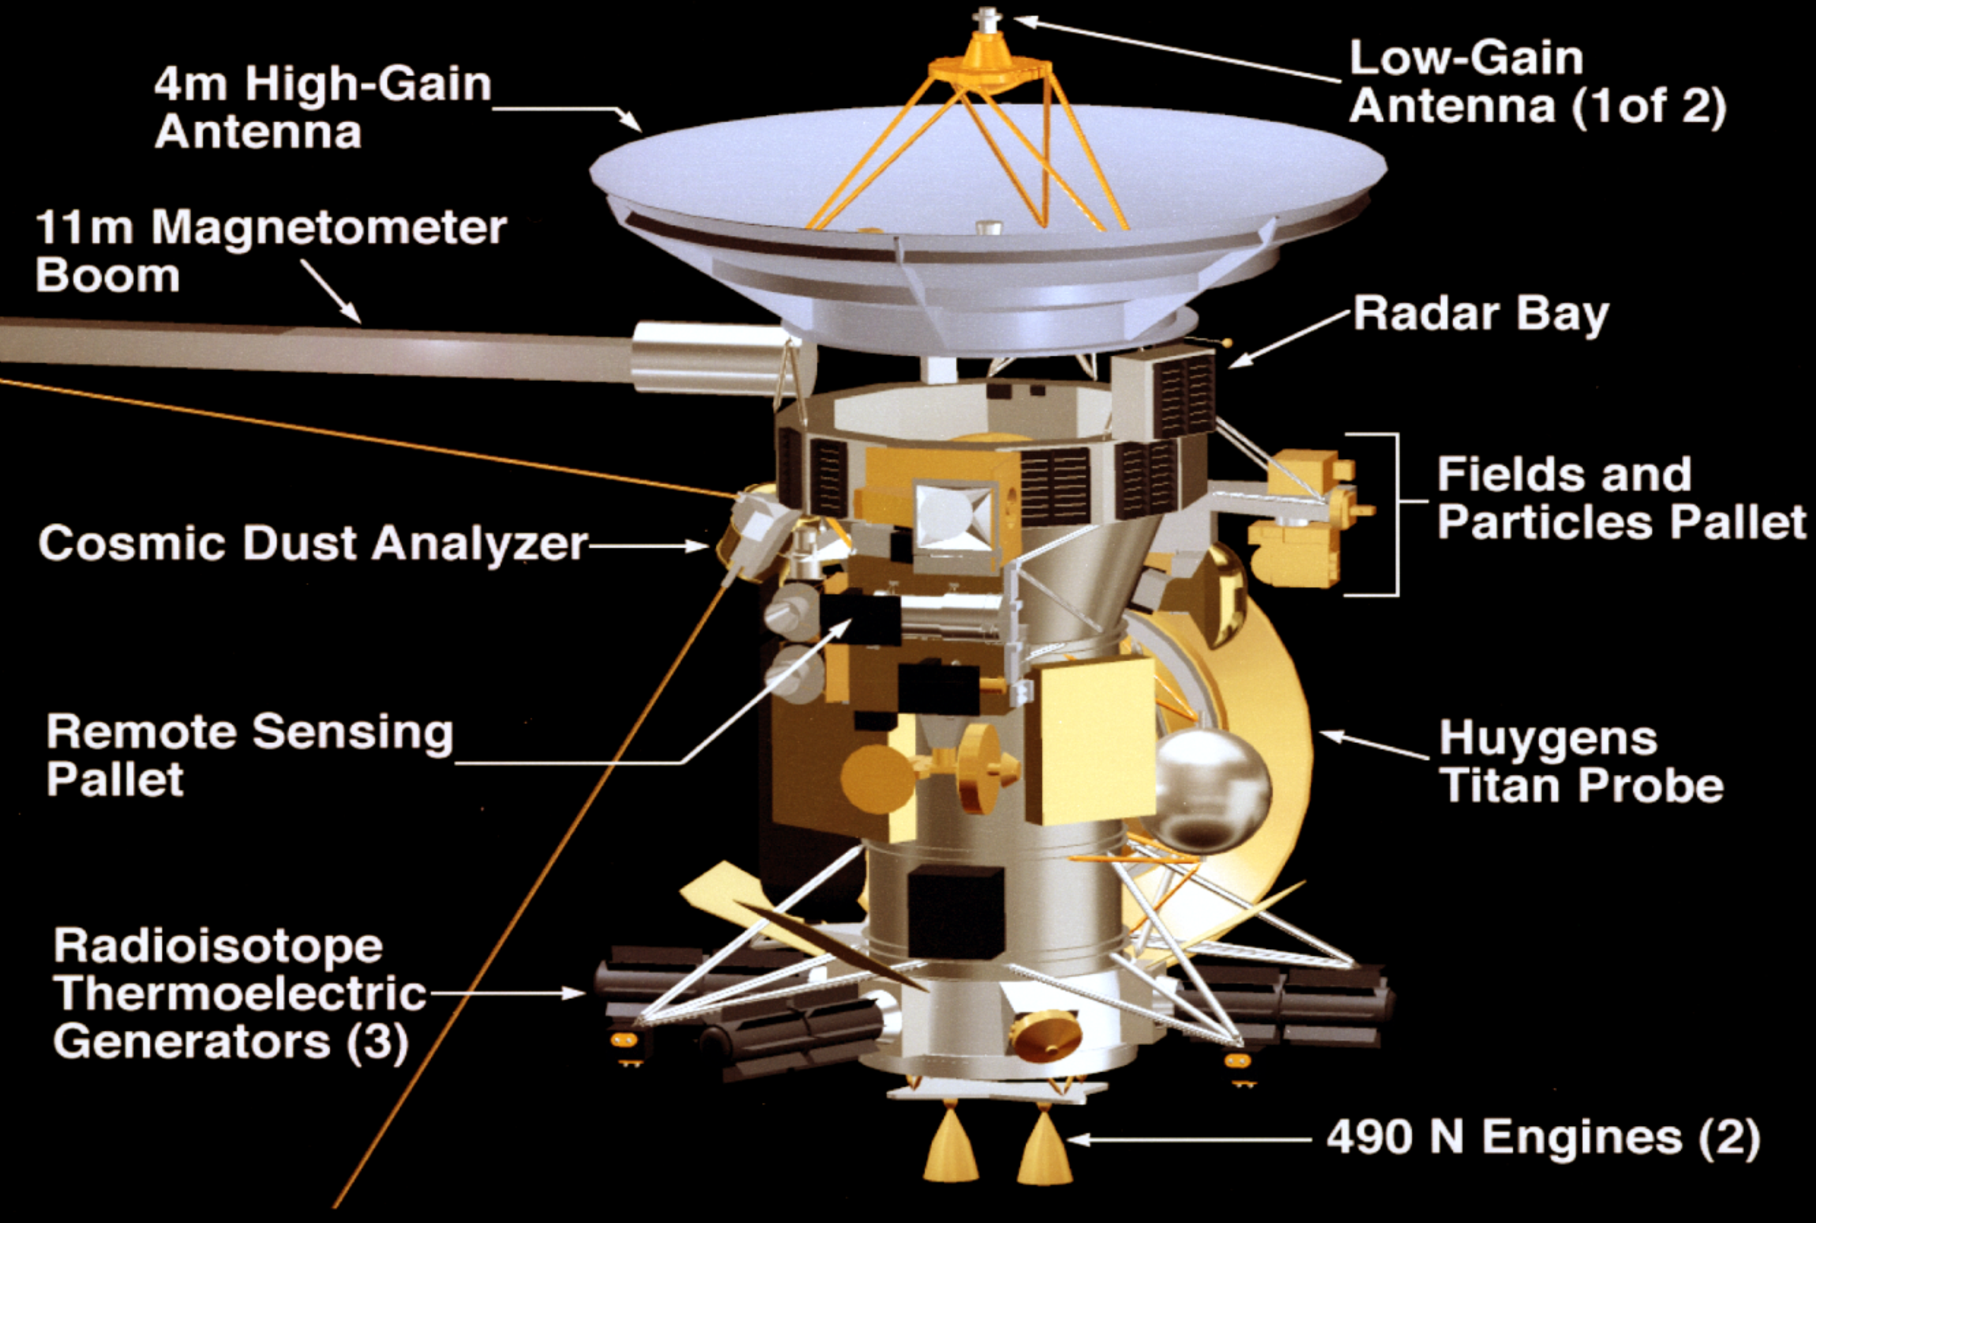
\includegraphics[width=1\textwidth]{cassini/spacecraft.pdf}
\caption[Diagram of the \textit{Cassini-Huygens} spacecraft]{Diagram of the \textit{Cassini-Huygens} spacecraft, from \citet{narvaez2004}. The spacecraft is about \SI{6.8}{m} in height.}
\label{cassini:fig:spacecraft}
\end{figure}

The \textit{Cassini-Huygens} mission (hereafter known as \textit{Cassini}) was a space mission designed to investigate the Saturn system, and was a collaboration between NASA, ESA and the Italian Space Agency (ASI). It was composed of a main \textit{Cassini} orbiter spacecraft with 12 instruments onboard, and the \textit{Huygens} probe with a further six, as described in \citet{matson2002}. A diagram of this spacecraft is shown in Figure~\ref{cassini:fig:spacecraft}. The instruments particularly relevant to the work in this thesis are discussed later in this chapter. 

Together, these instruments were designed such that the mission could investigate the entire Saturn system, from the interior of the planet itself to its atmosphere, rings, moons, and magnetosphere. The moon Titan was one of the key foci of the investigation, as it is the only moon in the solar system with a significant atmosphere, and it was initially thought to be a key source of plasma for the magnetosphere \citep{smith2004}. The \textit{Huygens} probe was therefore designed to detach from the main \textit{Cassini} orbiter and follow a single trajectory by parachute down to the surface of Titan, making \textit{in situ} measurements of Titan's atmosphere during the descent. The shield covering the \textit{Huygens} probe before it was deployed can be seen in Figure~\ref{cassini:fig:spacecraft}.

\section{Mission Timeline}\label{cassini:sec:timeline}
\textit{Cassini} launched from Cape Canaveral in Florida in October 1997, and finally arrived at the Saturn system in July 2004, after gravity-assist flybys of Venus, Earth and Jupiter. The mission was initially designed to operate for four years, from 2004-2008, and during this `Prime Mission' \textit{Cassini} completed 75 orbits of Saturn, and 44 flybys of Titan. The Prime Mission was incredibly successful, resulting in many exciting and unexpected discoveries about the Saturn system, such as the plumes of water being ejected from the icy moon Enceladus \citep{dougherty2006}. 

The mission was then extended by two years; the `Equinox Mission'. This extension allowed \textit{Cassini} to observe how the behaviour of the Saturn system changed with season, from northern winter to northern spring. (Saturn's obliquity relative to the ecliptic plane is \SI{26.7}{\degree}.) A Saturn year lasts 29 years, and the northern spring equinox occurred in August 2009, near the middle of the Equinox Mission. From a magnetospheric science perspective, equinox is a particularly interesting time to investigate the Saturn system, as the incident solar wind direction is parallel to Saturn's rotational/dipole equator, rather than at an angle slightly above or below. This means the solar wind conditions are approximately symmetrical in the northern and southern hemispheres, allowing for certain hemispheric effects, such as those discussed in Section~\ref{intro:sec:periodicities}, to be more readily investigated. Indeed, the data that are analysed in this thesis, particularly in Chapter~\ref{chap:equinox}, were acquired during \textit{Cassini's} Equinox Mission.

The mission was then further extended from 2010-2017, known as the `Solstice Mission', as the Saturn year continued into northern summer solstice in May 2017. The spacecraft trajectories were optimised to provide the most extensive coverage of scientifically interesting areas of the Saturn system, in the context of the entire mission. This culminated in the proximal orbits of the `Grand Finale', from April to September 2017. In each of these 22 final orbits, \textit{Cassini} traversed the gap between Saturn's atmosphere and the innermost ring, therefore orbiting far closer to the planet than at any other time in the mission, with a typical periapsis altitude of just ${\sim}\SI{2250}{km}$ above the 1-bar atmosphere level. This provided the opportunity to investigate scientific mysteries that still had not been answered from mission data so far, such as the core rotation rate of the planet and detailed internal magnetic field structure. The \textit{Cassini} mission then ended on 15 September 2017, as the spacecraft plunged into the planet's atmosphere and lost contact with Earth. The Grand Finale was designed in this way not just for maximum scientific reward, but also because the onboard rocket propellant used to manoeuvre the spacecraft was running out. With \textit{Cassini's} discovery of a likely sub-surface water ocean at Enceladus, and also prebiotic chemistry at Titan, the mission could not risk the spacecraft accidentally crashing into one of these moons and potentially contaminating them with Earth-based life forms. It was therefore necessary to deliberately impact the spacecraft into the planet Saturn itself.

\begin{figure}
\centering
\noindent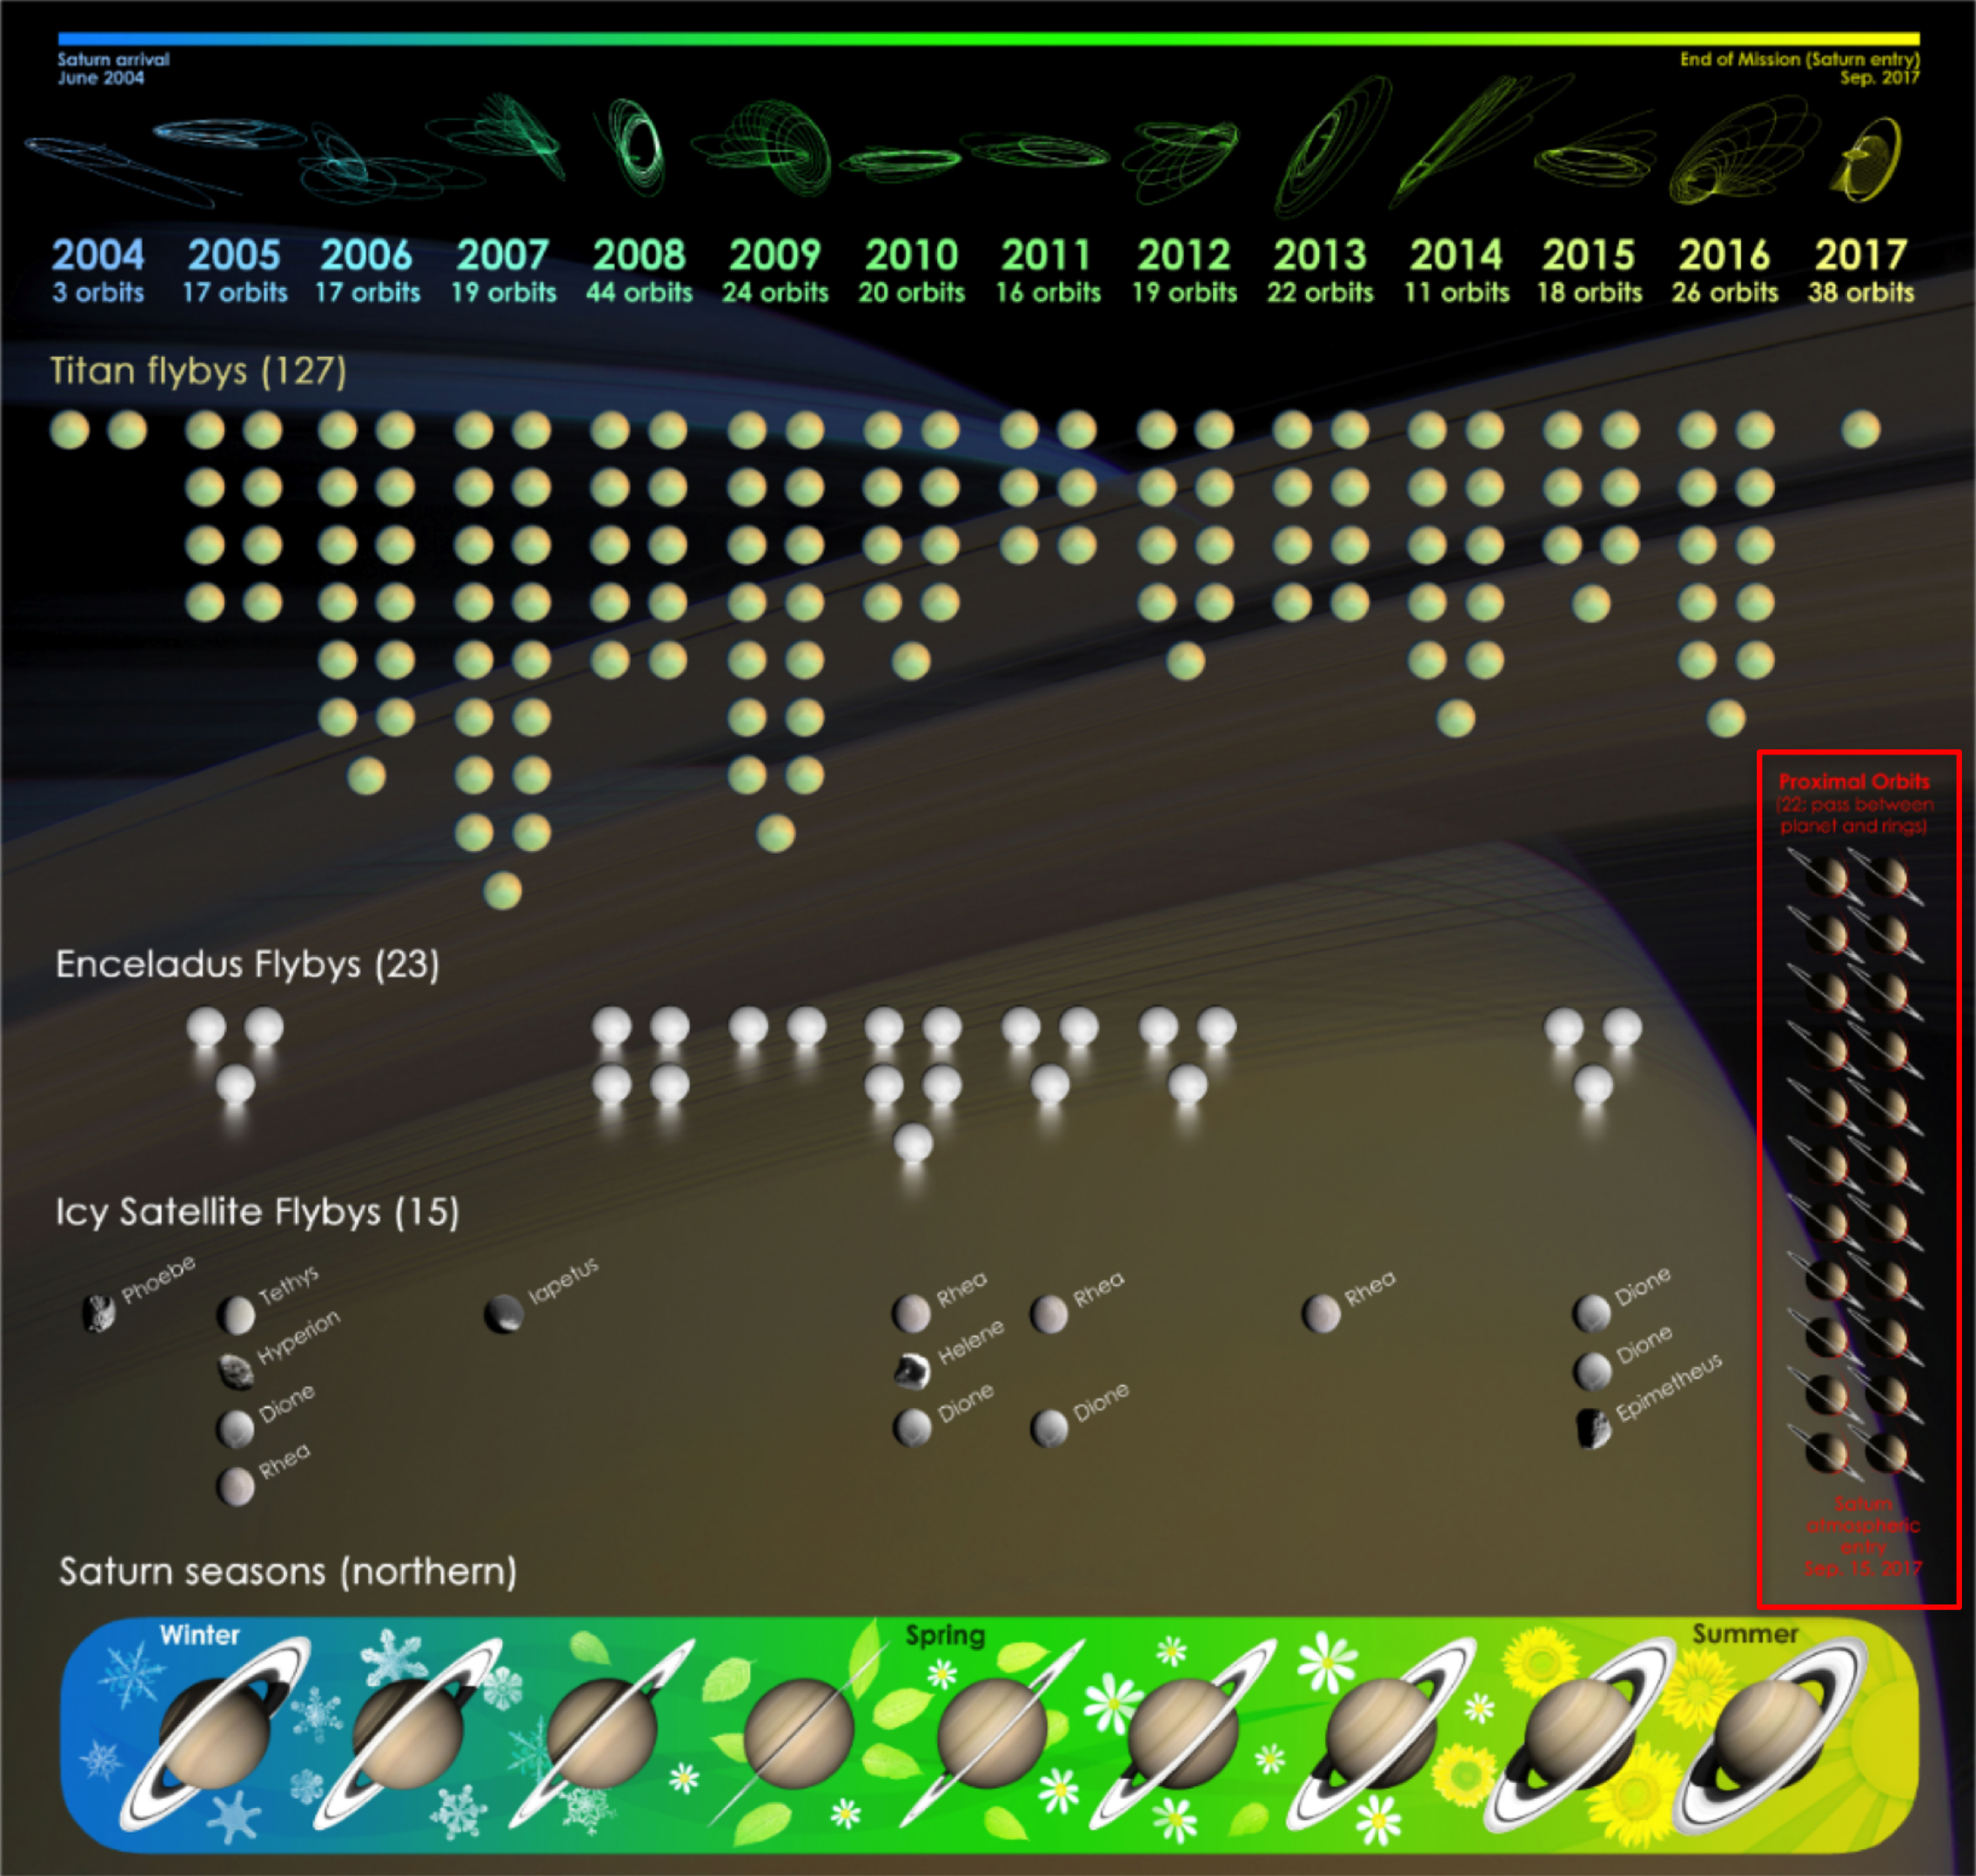
\includegraphics[width=0.9\textwidth]{cassini/mission_overview.jpg}
\caption[Diagram showing overview of \textit{Cassini }space mission.]{Diagram showing overview of \textit{Cassini} space mission orbit trajectories and moon flybys, from \citet{nasa2017}.}
\label{cassini:fig:missionoverview}
\end{figure}

Figure~\ref{cassini:fig:missionoverview} shows an overview of the entire \textit{Cassini} mission. At the top of the image the trajectories of the orbits are depicted, showing the extensive coverage \textit{Cassini} made in radial distance, latitude and local time. Also shown are the number of flybys of various moons, and  at the bottom the Saturn season is depicted. The proximal orbits, shown in red, are barely visible as they are so close to the Saturn surface.

\section{Key Instruments}
\subsection{Magnetometer (MAG)}
The dual technique magnetometer system (MAG) measured the magnitude and direction of Saturn's magnetic field \textit{in situ}, described in \citet{dougherty2004} and summarised here. The system was composed of a Vector/Scalar Helium Magnetometer (V/SHM), located at the end of the \SI{11}{m} long boom shown in Figure~\ref{cassini:fig:spacecraft}, and a FluxGate Magnetometer (FGM), located half way along it. This positioning was chosen so that measurements were contaminated as little as possible by magnetic fields generated by other instruments and electronics subsystems onboard the spacecraft itself, and also so that measurements from the two instruments could be compared for calibration. However the V/SHM malfunctioned early on in the mission, in November 2005, and so all the data presented in this thesis were measured solely by the FGM.

\begin{figure}
\centering
\noindent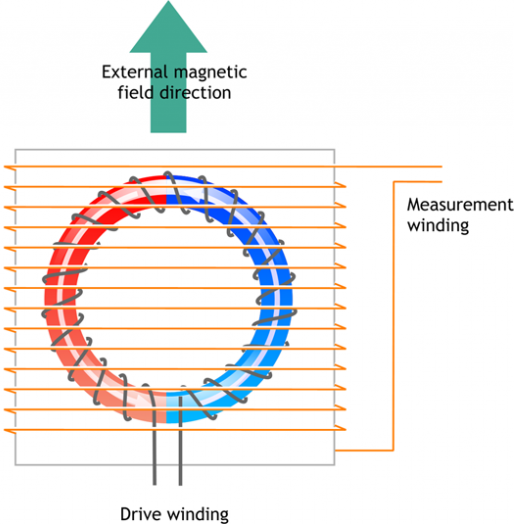
\includegraphics[width=0.6\textwidth]{cassini/FGMdiagram.png}
\caption[Diagram of how a fluxgate magnetometer works.]{Diagram showing basic construction of a fluxgate magnetometer, from \citet{carisma2018}. The drive winding and measurement winding are shown in dark grey and orange, respectively. The magnetic field induced in the core due to the current in  the drive winding  is shown by  the pale arrows on top of  the blue and red halves of the  core. The external magnetic field direction is shown by the large green arrow.}
\label{cassini:fig:FGMdiagram}
\end{figure}

The FGM was composed of three fluxgate sensors positioned orthogonally to each other, to measure the three vector components of the ambient magnetic field. A diagram showing the basic construction of one such sensor is shown in Figure~\ref{cassini:fig:FGMdiagram}. In each sensor, a coil of wire (`drive winding' in Figure~\ref{cassini:fig:FGMdiagram}) was wound around a high permeability ring-shaped core. A \SI{15.625}{\hertz} square wave current flowed through this drive coil, in order to induce a magnetic field in the core with clockwise orientation as shown by the pale arrows, until the core was saturated. Surrounding this entire set up was another coil of wire (`measurement winding' in Figure~\ref{cassini:fig:FGMdiagram}). In the absence of an external magnetic field, the two halves of the core shown in Figure~\ref{cassini:fig:FGMdiagram} would go into and out of saturation at the same time due to the drive winding current, and so there would  be no change of  flux through the measurement winding. However in the presence of an external magnetic field  oriented as shown by  the green arrow, one half of the core would become saturated more quickly than the other (depending on the phase of the drive winding current), causing a net change in magnetic flux through the measurement winding. In accordance with Faraday's law of  induction, this  would induce a voltage in  the measurement winding,  which could then be calibrated and used to measure the magnitude  of the external magnetic field. 

Only the component of the magnetic field perpendicular to the measurement winding orientation can be detected by this process, hence the need for three orthogonally positioned sensors. These three sensors were mounted on a single ceramic block, with the entire FGM  instrument  weighing just \SI{0.44}{kg}. The material ceramic was chosen for its low thermal expansion coefficient,  meaning  it changes shape very little under  changes in ambient temperature, and so any misalignment between the sensors was minimised.

The FGM had multiple operational ranges depending on the likely ambient magnetic field strength, which it could switch between automatically, and had a digital resolution of approximately one part in 10,000 depending on the range. The four ranges were $\pm\SI{40}{nT}$, $\pm\SI{400}{nT}$, $\pm\SI{10000}{nT}$, and $\pm\SI{44000}{nT}$, necessary for sampling different regions of Saturn's magnetosphere, where the magnetic  field strength  varies over many orders of magnitude. The normal downlink data rate for the FGM was $\SI{32}{vectors/s}$, although in this thesis we only investigate large-scale magnetospheric structures on large timescales, and so only present 1-hour-averaged MAG data. Such \textit{In situ} observations of Saturn's magnetic field revealed detailed information about the structure of Saturn's magnetosphere, such as the dynamical current sheet behaviour \citep[e.g.][]{provan2012}, and were also used to demonstrate the existence of an atmospheric plume at the icy moon Enceladus \citep{dougherty2006}. In Chapter~\ref{chap:equinox}, we use 1-hour-averaged MAG data measured near Saturn equinox in late 2009 to investigate the periodic flapping and breathing of Saturn's equatorial current sheet.

\subsection{Magnetospheric Imaging Instrument (MIMI)}
The Magnetospheric Imaging Instrument (MIMI) was a system for detecting both neutral and charged particles with high energies, described in \citet{krimigis2004} and summarised here. It was composed of three separate instruments, each described below.
\subsubsection{Ion and Neutral Camera (INCA)}
The Ion and Neutral Camera (INCA) was designed to detect both energetic neutral atoms (ENAs) and ion species over the range of energies $0.007{\--}\SI{3}{MeV/nucleon}$, and used time-of-flight information to determine the particle's energy and incident direction. A simple diagram of the instrument is shown in Figure~\ref{cassini:fig:INCAinstrument}.

\begin{figure}
\centering
\noindent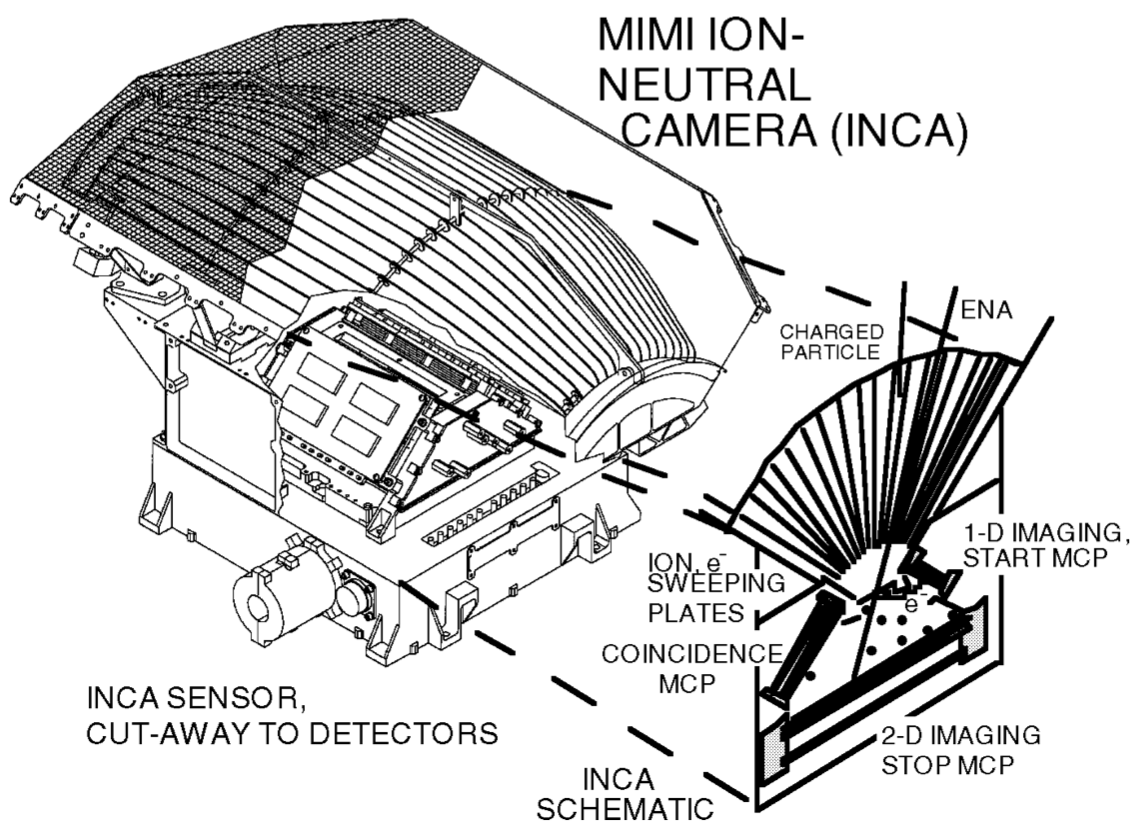
\includegraphics[width=0.8\textwidth]{cassini/INCAinstrument.png}
\caption[Diagram of the MIMI/INCA instrument.]{Cutaway diagram of the MIMI/INCA instrument, from \citet{krimigis2004}.}
\label{cassini:fig:INCAinstrument}
\end{figure}

Particles detected by the instrument would arrive broadly from above in the frame of  in Figure~\ref{cassini:fig:INCAinstrument}, and pass through the fan-like arrangement of serrated collimator plates, labelled as `ION, e- SWEEPING PLATES'. When in `neutral mode', these plates would be alternately charged at $\pm\SI{6}{kV}$ in order to sweep any energetic charged particles (with energies $\leq \SI{500}{keV}$) into the plate walls, thus excluding them from the internal detector. ENAs meanwhile would pass through the region unperturbed, and then penetrate a thin foil layer covering  the entrance slit. This would generate secondary electrons in the foil, which were steered to a 1-D microchannel plate (MCP) labelled as `1-D IMAGING, START MCP' in  Figure~\ref{cassini:fig:INCAinstrument}, recording the entrance position of the ENA and start time of travel. As the ENA proceeded further to the back of the instrument, it would penetrate another thin foil layer and  encounter a 2-D microchannel plate, labelled `2-D IMAGING STOP MCP', recording the exit position (in 2-D) and the end time of travel. At the same time, secondary electrons generated in the second thin foil layer would be steered to the microchannel plate  labelled `COINCIDENCE MCP', enabling a comparison with  the detection of the other plate in order to reduce background measurement noise. From all this information, the energy, mass, and incident direction of the ENA could be deduced. In particular it was found that the number of electrons generated in the foil was proportional to the mass of  the incident particle, which enabled the species (e.g.\ oxygen or hydrogen) of the particle to be determined. 

When operating in `ion mode', the  charge on the sweeping plates would be switched to zero so that ions could enter, and the instrument would detect ion species in a similar way. Neutrals would still also be able to enter the instrument in this mode, but in general the neutral counts were much lower and so would be drowned out by the incident ions.

\begin{figure}
\centering
\noindent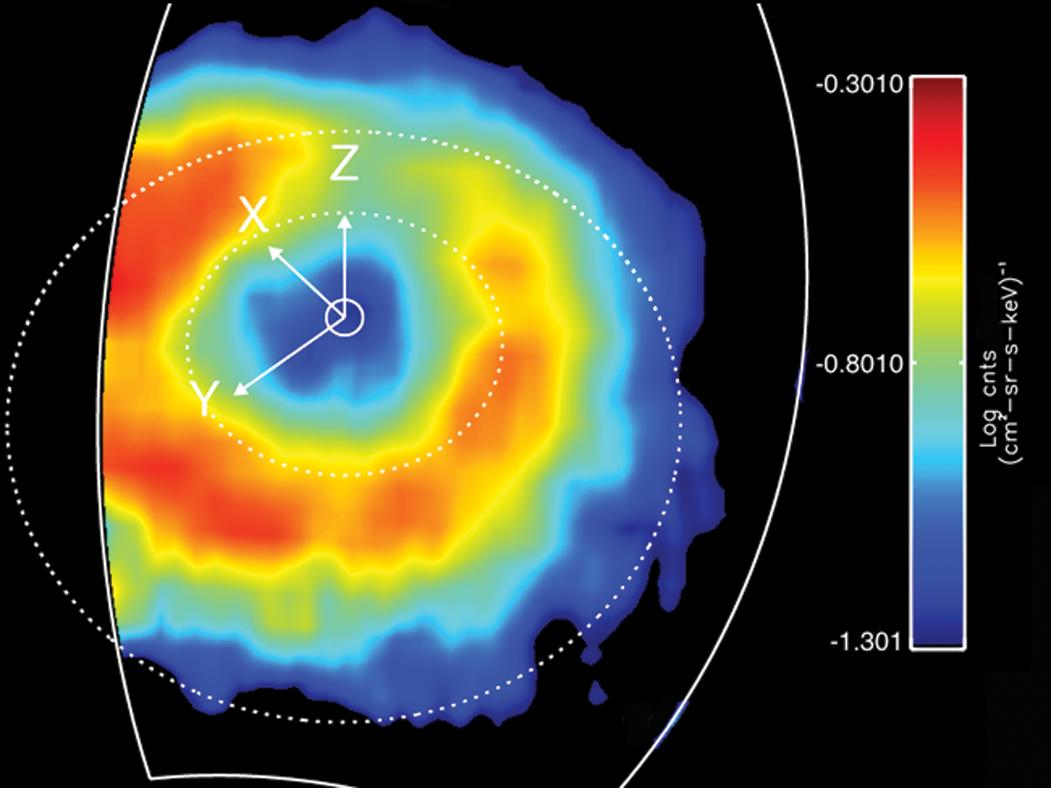
\includegraphics[width=0.8\textwidth]{cassini/INCAringcurrent.jpg}
\caption[ENA image of Saturn's ring current from MIMI/INCA.]{ENA image of Saturn's ring current from the MIMI/INCA instrument as viewed from a latitude of \SI{55}{\degree} above the northern hemisphere, averaged over a 3 hour period on 19 March 2007, from \citet{nasa2007}. Colour shows ENA intensity as per the colour bar. Saturn is at the  centre, and the white dashed lines show the orbits of the moons Rhea (\SI{8.7}{R_S}) and Titan (\SI{20.2}{R_S}). The Z axis points along Saturn's dipole/spin axis, the Y axis points approximately towards dusk, and the X axis points approximately  towards the Sun. The MIMI/INCA field of view is shown by the solid white line.}
\label{cassini:fig:INCAringcurrent}
\end{figure}

At Saturn, ENAs can be produced via charge exchange between singly-charged energetic ions and Saturn's neutral gas distribution (which originates from Saturn's rings and moons). Through collisions, an energetic ion can `steal' an electron from a neutral particle, such that the ion becomes neutral and is no longer constrained by the planetary magnetic field, and thus subsequently travels through space unperturbed. The energetic ions that make up Saturn's equatorial ring current can therefore be traced remotely via detection of ENAs originating from the equatorial plane. Figure~\ref{cassini:fig:INCAringcurrent} shows such an ENA image taken by \textit{Cassini's} MIMI/INCA instrument  on 19 March 2007, clearly showing the substantial ring current structure. 

\subsubsection{Charge-Energy-Mass Spectrometer (CHEMS)}
\begin{figure}
\centering
\noindent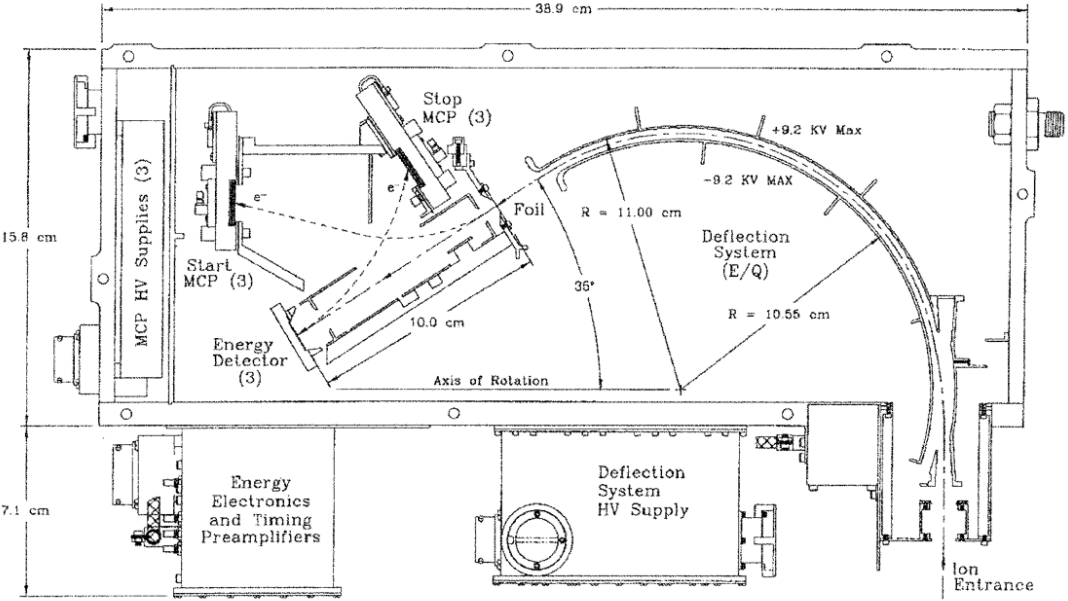
\includegraphics[width=0.9\textwidth]{cassini/CHEMSdiagram.png}
\caption[Diagram of the MIMI/CHEMS instrument.]{Diagram of the MIMI/CHEMS instrument, from \citet{krimigis2004}.}
\label{cassini:fig:CHEMSdiagram}
\end{figure}

The CHEMS instrument was designed to measure the charge, energy and mass of energetic ions, in the energy range $3{\--}\SI{220}{keV/e}$, using electrostatic deflection and time-of-flight information. The  instrument was mounted on \textit{Cassini} on the fields and particles pallet labelled in Figure~\ref{cassini:fig:spacecraft}. This positioning, combined  with the instrument construction described below, meant that during a spacecraft roll the instrument would have almost $4\pi$ steradian viewing geometry. This enabled the capability of measuring 3-D distribution functions of the energetic ion populations. A diagram of the instrument is shown in Figure~\ref{cassini:fig:CHEMSdiagram}.

As an ion entered the instrument from below in the frame on Figure~\ref{cassini:fig:CHEMSdiagram}, it would first encounter the `Deflection System', consisting of two oppositely charged spherical plates as shown in the diagram. The voltage across the plates was stepped through a series of logarithmically spaced  values over time to a maximum  of $\pm\SI{9.2}{keV}$, such that the plates acted as an energy per charge ($E/Q$) filter, allowing only ions within a small $E/Q$ band to pass through the system at any given time. If transmitted, the ion would then penetrate a thin foil layer, generating  secondary electrons that are then steered to the `Start MCP' microchannel plate, which would enable a start time-of-flight calculation to be made, as for MIMI/INCA. The ion would then impact the solid-state detector, labelled as `Energy Detector' in Figure~\ref{cassini:fig:CHEMSdiagram}, generating  secondary electrons that would then be steered to the `Stop MCP',  for the time-of-flight calculation. The solid-state detector also measured the residual energy of the incoming ion, so that the charge could be ascertained from the initial $E/Q$ measurement. Three independent telescopes with different viewing angles were included in CHEMS, hence the `(3)' labels at the energy detector, in order to enable the  aforementioned coverage of viewing geometry.

In combination with the other instruments that make up MIMI, MIMI/CHEMS was used to detect the widespread presence of energetic oxygen (O$^+$) and hydrogen (H$^+$) ions in Saturn's equatorial magnetosphere, and  to determine the partial pressures associated with the two populations \citep[e.g.][]{sergis2009}. The influence of his hot plasma population on the large-scale structure of the magnetosphere is discussed and investigated at length in this thesis, in particular in Chapters~\ref{chap:compress} and \ref{chap:LTsectors}.

\subsubsection{Low-Energy Magnetospheric Measurement System (LEMMS)}
\begin{figure}
\centering
\noindent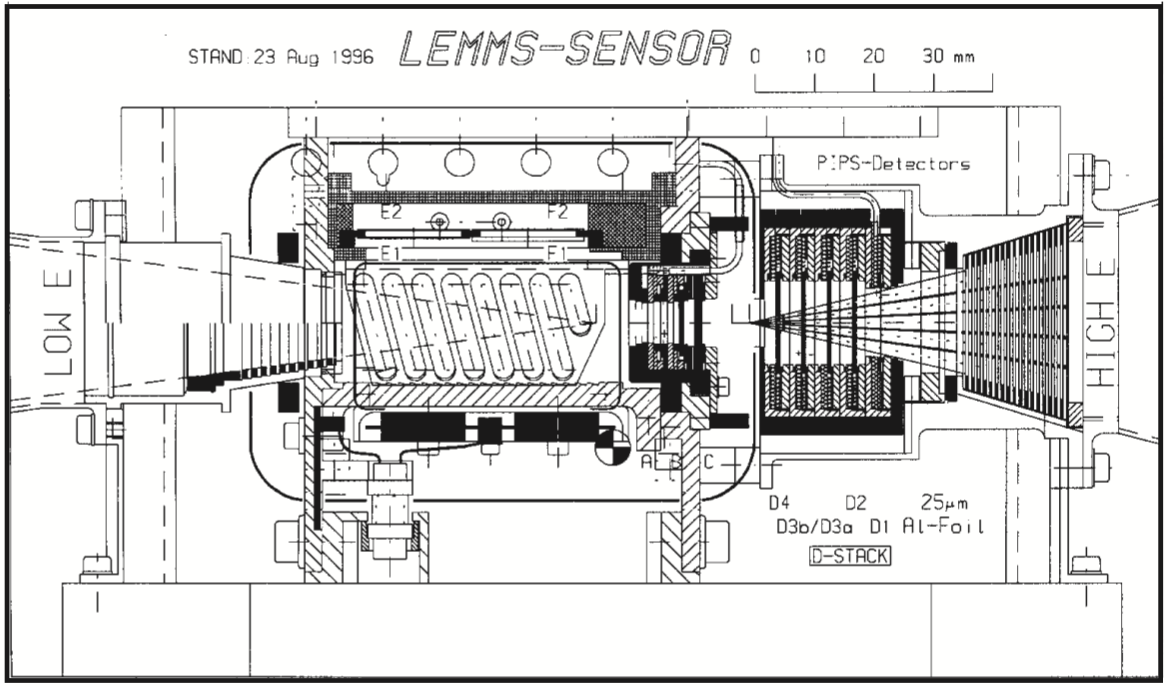
\includegraphics[width=0.9\textwidth]{cassini/LEMMSdiagram.png}
\caption[Diagram of the MIMI/LEMMS instrument.]{Diagram of the MIMI/LEMMS instrument, from \citet{krimigis2004}.}
\label{cassini:fig:LEMMSdiagram}
\end{figure}

The LEMMS instrument was designed to measure the distribution of energetic ion and electron fluxes. The instrument consisted of two oppositely oriented telescopes; a low-energy end, which measured ions with $E>\SI{30}{keV}$ and electrons with $E=\SI{15}{keV}{\--}\SI{1}{MeV}$, and a high-energy end, which measured ions with $E=1.5{\--}\SI{160}{MeV}$ and electrons with $E=0.1{\--}\SI{5}{MeV}$. The entire assembly was shielded with a platinum cover to avoid particles with energies $E<\SI{30}{MeV}$ penetrating the sides of the instrument. The instrument was mounted on a rotating platform to enable a larger total field of view; however, this mobility became compromised early on in the mission (early 2005), and so it remained in a fixed orientation with field of view closely aligned with one of the MIMI/CHEMS telescopes for the remainder of the mission. A diagram of the instrument is shown in Figure~\ref{cassini:fig:LEMMSdiagram}.

In the low-energy telescope (labelled `LOW E' on the left of Figure~\ref{cassini:fig:LEMMSdiagram}, an internal permanent magnet provided an inhomogeneous magnetic field, which separated the incoming ions and electrons that had passed into the instrument through the initial collimator. The electrons would be more strongly perturbed by the magnetic field than the ions, and so would be diverted to the semiconductor silicon detectors labelled E(1,2) and F(1,2), depending on their initial energies and incident directions. Incident ions, which are less strongly perturbed by in the presence of a magnetic field due to their higher mass (as discussed in this thesis, Section~\ref{intro:sec:singleparticle}), would proceed to the back of the instrument and strike the detectors labelled A and B. Data from the detectors could then be used to determine the energies of the incoming particles. 

In the high-energy telescope, a stack of detectors labelled D(1,2,3a,3b,4) detected incoming ions and electrons that had passed through the initial collimator on that side (plus a thin layer of aluminium foil, labelled `Al-Foil', included to prevent contamination from sunlight and lower energy ions). The combination of detections from the different detectors, which had different electronic thresholds, could then be used to distinguish ions and electrons. Between detectors B on the low-energy side and D4 on the high-energy side, a gold absorber labelled C was included to prevent lower energy ions penetrating through to the high-energy detectors.

Information from this instrument was used in combination with MIMI/CHEMS to characterise the distributions of the high energy plasma population in Saturn's magnetosphere, for example in \citet{sergis2017}. In Chapter~\ref{chap:LTsectors}, we use observations from this study in particular as inputs to the UCL/AGA magnetodisc model, in order to investigate how this hot plasma population influences magnetodisc structure at different local times.

\subsection{Plasma Spectrometer (CAPS)}
\begin{figure}
\centering
\noindent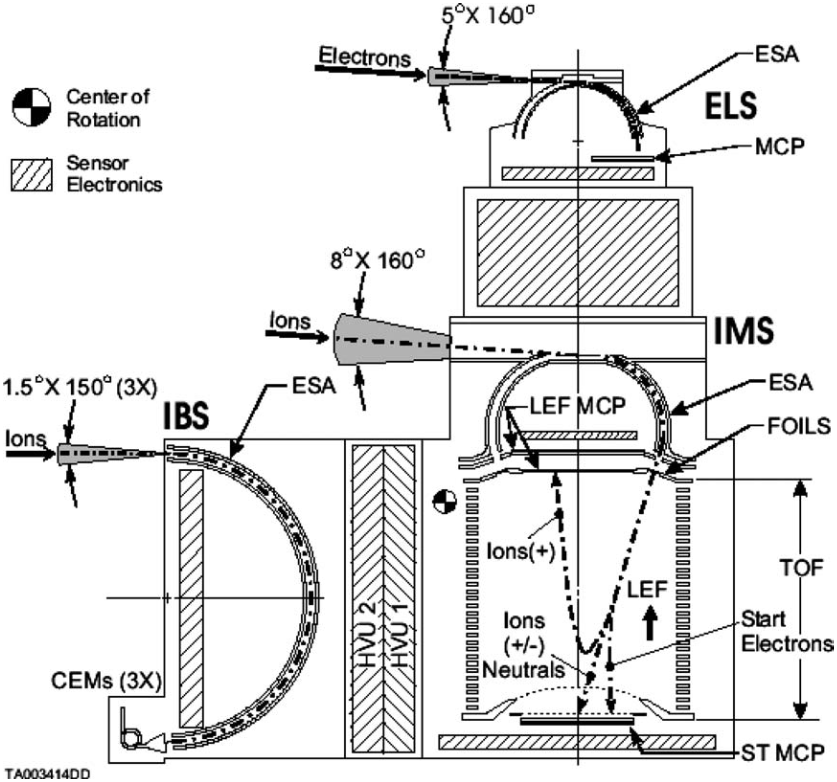
\includegraphics[width=0.8\textwidth]{cassini/CAPSdiagram.png}
\caption[Diagram of the CAPS instrument.]{Diagram of the CAPS instrument, from \citet{young2004}. The dot-dashed lines show the general shape of particle trajectories.}
\label{cassini:fig:CAPSdiagram}
\end{figure}

The CAPS instrument was used to measure the distributions of ions and electrons at lower energies than those observed by the MIMI instrument, and is described in \citet{young2004} and summarised here. It was made up of three separate sensors, including an electron spectrometer (ELS), ion mass spectrometer (IMS), and ion beam spectrometer (IBS), which is not discussed here as it was not used to make observations relevant to this thesis. ELS could detect electrons with energies in the range ${0.6}{-}\SI{29000}{eV}$, and IMS could detect ions in the range ${1}{-}\SI{50000}{eV}$. A diagram of the instrument is shown in Figure~\ref{cassini:fig:CAPSdiagram}. The entire instrument was mounted on a rotating platform on the underside of the `fields and particles pallet' shown in Figure~\ref{cassini:fig:spacecraft}, such that it had almost $2\pi$ steradians field of view, when not partially blocked by other parts of the spacecraft.

At both ELS and IMS, incoming particles first travelled between separated curved charged plates, labelled `ESA' (electrostatic analyser) in the diagram. As in the MIMI/CHEMS instrument, the voltage across the plates was stepped through a series of logarithmically spaced values over time, in order to filter only charged particles within a certain small range in $E/Q$ at a given time. 

For ELS, this corresponds to filtering for different energy electrons, as $Q$ is fixed for electrons. The angular distribution of the incoming electrons at each energy range was then determined based on where the electrons hit the microchannel plate, labelled `MCP' in Figure~\ref{cassini:fig:CAPSdiagram}. 

For IMS, the instrument performed time-of-flight calculations to determine the particle energies. The region labelled as `TOF' was charged at $\SI{-14.6}{kV}$ at the top, and $\SI{+14.6}{kV}$ at the bottom, generating a linear electric field labelled `LEF'. This would first accelerate ions that successfully exited the charged plates out through one of eight carbon foils, labelled `FOILS', generating secondary electrons to be steered to a microchannel plate to measure the start time of flight, as in the MIMI/INCA and CHEMS instruments. Positive ions with energies below ${\sim}\SI{15}{keV}$ would then be reflected back by the linear electric field into the `LEF MCP', while more energetic ions would be slowed down but still eventually penetrate the `straight-through' microchannel plate, labelled `ST MCP'. Molecular ions would break up on penetrating the initial carbon foils, but the resulting daughter products would still behave in this way and thus could be detected, and relevant information used to infer the original source particle. The peaks in the observed time-of-flight spectra would correspond to given ion mass-to-charge ratios $M/Q$, such that different ion species could then be identified.

Due to a technical fault, CAPS was switched off permanently in 2012. However, up until that time, observations made by the instrument were useful for investigating many magnetospheric phenomena at Saturn. Pertinent to this thesis, CAPS/ELS observations were used by \citet{pilkington2015} to identify instances when \textit{Cassini} crossed Saturn's magnetopause boundary, between the magnetosphere and the magnetosheath, as the sheath typically contains a more dense and lower energy population of electrons than the magnetosphere. This development of a database of crossings enabled a study of how the shape and size of the magnetopause surface varied under different conditions, and is complemented by the modelling study discussed in Chapter~\ref{chap:equinox}.

\section{Summary}
The \textit{Cassini} space mission has, without a doubt, revolutionised our understanding of the large-scale structure and dynamics of Saturn's magnetosphere. Throughout this thesis, we refer to important results based on observations from the \textit{Cassini} instruments we have described herein. In addition, the \citet{achilleos2010a} model discussed in Section~\ref{intro:sec:forcebalancemodel} uses results from these instruments as equatorial boundary conditions. In the first study discussed in this thesis, we explore the influence of the variable hot plasma population detected by the MIMI instrument on the compressibility of Saturn's dayside magnetosphere.
\chapter[The Compressibility of Saturn's Magnetosphere]{The Compressibility of Saturn's Magnetosphere in Response to Internal and External Influences}
\label{chap:compress}

In this chapter, we present the results  of an investigation into the compressibility of Saturn's dayside magnetosphere in response to changing internal  and external influences. These influences include the global hot plasma content in the magnetosphere, which inflates the magnetosphere and  enhances the ring current activity, and the external solar wind dynamic pressure $D_\mathrm{P}$, which controls the overall system size. Previous empirical studies assumed that Saturn's magnetopause stand-off distance varies as $D_\mathrm{P}^{-1/\alpha}$, and measured a constant compressibility parameter $\alpha$ corresponding to behaviour intermediate between a vacuum dipole appropriate for Earth ($\alpha \approx 6$), and a more easily compressible case appropriate for Jupiter ($\alpha \approx 4$). In this chapter we employ the 2-D force-balance model of Saturn's magnetodisc from \citet{achilleos2010a}, described in Section~\ref{intro:sec:forcebalancemodel} of this thesis, to investigate relationship in response to changes in $D_\mathrm{P}$ and global hot plasma content. For hot plasma levels compatible with Saturn observations, we model the magnetosphere at a range of stand-off distances and estimate the corresponding $D_\mathrm{P}$ values by assuming pressure balance across the magnetopause boundary. We find that for `average' hot plasma levels, our estimates of $\alpha$ are not constant with $D_\mathrm{P}$, but vary from ${\sim}4.8$ for high $D_\mathrm{P}$ conditions, when the magnetosphere is compressed (${\leq}\SI{25}{R_S}$), to ${\sim}3.5$ for low $D_\mathrm{P}$ conditions. This corresponds to the magnetosphere becoming more easily compressible as it expands. We also find that enhanced global hot plasma content increases magnetospheric compressibility even at fixed $D_\mathrm{P}$, with $\alpha$ estimates ranging from ${\sim}5.4$ to ${\sim}3.3$ across the range of our parameterised hot plasma content. We suggest that this behaviour is predominantly driven by reconfiguration of the magnetospheric magnetic field into a more disc-like structure under such conditions. In a broader context, the compressibility of the magnetopause reveals information about global stress balance in the magnetosphere, which we discuss in this chapter. The contents of this chapter are heavily based on the published study \citet{sorba2017}.

\section{Introduction}\label{compress:sec:intro}
We discussed in Chapter~\ref{chap:intro} how in a steady-state system, the shape and size of a planetary magnetopause is determined by pressure balance across the boundary, between the internal magnetic and plasma pressures of the magnetosphere, and the pressure associated with the shocked solar wind plasma of the magnetosheath. The pressure exerted by the solar wind is principally due to the component of the dynamic pressure $D_\mathrm{P}$ that is normal to the magnetopause surface, where $D_\mathrm{P}$ is defined as $\rho_mu_\mathrm{SW}^2$ ($\rho_m$ denotes solar wind mass density and $u_\mathrm{SW}$ is the velocity). The dayside magnetosphere is compressed when the upstream dynamic pressure increases, and inflates when the dynamic pressure drops. The magnetopause is therefore in constant motion, with a velocity of order {\SI{10}{km s^{-1}}} for Earth's magnetopause {\citep{berchem1982}}, and {\SI{100}{km s^{-1}}} for Saturn's {\citep{masters2011}}. However to first order, its location can be approximated by assuming Newtonian pressure balance across the surface. 

A useful proxy of the overall size scale of a magnetosphere is the `stand-off distance', $R_\mathrm{MP}$. This is the location of the magnetopause boundary measured from the planet center along the planet-Sun line, i.e. the sub-solar nose of the magnetosphere. At this point, the solar wind flow direction is perpendicular to the magnetopause surface, and so the pressure balance relation defined in Equation~\ref{intro:eq:pbalance2} simplifies to
\begin{equation}\label{compress:eq:pbalance}
\frac{B_{\mathrm{MS}}^2}{2\mu_0} + P_{\mathrm{MS}} = kD_\mathrm{P}.
\end{equation}
$B_\mathrm{MS}$ is the magnetic field strength just inside the magnetopause boundary, which comprises the internal planetary field and other sources, such as the field associated with a magnetospheric ring current. $P_{\mathrm{MS}}$ is the total plasma pressure just inside the magnetopause boundary, the relative significance of which varies greatly between planets, as discussed in Section~\ref{intro:sec:comparativemagnetospheres}. $k$ is a positive constant $\leq1$ to account for the diversion of solar wind flow around the magnetospheric obstacle, and depends on the ratio of specific heats $\gamma$ in the solar wind, and the upstream sonic Mach number $M$. 

A key source of pressure inside all planetary magnetospheres is the magnetic pressure $P_\mathrm{B}=B_\mathrm{MS}^2/2\mu_0$. We can therefore estimate the value of $R_\mathrm{MP}$ to first order, by finding the radial distance from the planet center $r$ at which the magnetic pressure is  balanced by the solar wind dynamic pressure. If we make the assumption $B \propto r^{-\chi}$, such that the magnetic pressure $P_\mathrm{B} \propto r^{-2\chi}$, we can then write
\begin{equation}\label{compress:eq:key}
R_\mathrm{MP}=a_1D_\mathrm{P}^{-1/\alpha}
\end{equation}
where $a_1$ is a constant that determines the size scale of the system and $\alpha$ is the `compressibility parameter', equal to $2\chi$. This relationship is used to model the overall size of the magnetosphere in studies of the planets Earth, Jupiter and Saturn, as described in detail below. 

% In particular it was discovered by the \textit{Cassini} space mission that the icy moon Enceladus, which orbits Saturn at a distance of \SI{3.95}{R_S} (\si{R_S} = Saturn's equatorial radius, \SI{60268}{km}), ejects plumes of water group molecules into the magnetosphere at around \SI{300}{kg s^{-1}}, which are then ionized and form a wide torus of plasma around the planet \citep{dougherty2006, tokar2006, bagenal2011}. This dense plasma is accelerated to corotation with the rapidly rotating magnetosphere, producing a significant centrifugal force which is directed radially outwards on the plasma in its corotating frame of reference. In order for the magnetic tension force to balance this centrifugal force in Saturn's outer magnetosphere, the magnetic field lines may be pictured as being `stretched' radially outwards near the equatorial plane, from a dipole structure into a more `disk-like' structure, supported by a corresponding azimuthal ring current.

For a vacuum dipole magnetic field $\chi=3$, giving $\alpha=6$. This is broadly consistent with observations of Earth's magnetosphere, such as \citet{shue1997}. However in contrast to the terrestrial system, Saturn's magnetosphere has significant internal plasma sources; a cold population originating from the icy moon Enceladus \citep[e.g.][]{dougherty2006,tokar2006}, and a hotter population that is more variable with radial distance and over time \citep[e.g.][]{sergis2009}. Saturn also rotates more rapidly  than the Earth, with a ${\sim}\SI{10.7}{hour}$ period \citep{desch1981}. As discussed in detail in Sections~\ref{intro:sec:comparativemagnetospheres} and \ref{intro:sec:saturn}, these conditions causes Saturn's magnetosphere to form a more `disc-like' configuration, with magnetic field lines `stretched' radially outwards near the equatorial plane, supported by an azimuthal ring current. This magnetic field configuration affects the compressibility parameter $\alpha$, since for a disc-like magnetic field, $B$ varies more slowly with radial distance in the outer magnetosphere than for a dipole. This can be seen in Figure~\ref{compress:fig:magdata}, which shows the total magnetic field strength measured by the \textit{Cassini} MAG instrument in Saturn's dayside magnetosphere, taken from 3 equatorial orbits during Saturn equinox (Revs $120{\--}122$, 23~October to 17~December~2009). In the inner and middle magnetosphere the data appear to be well approximated by the relationship $B \propto r^{-3}$. However in the outer magnetosphere ($r \gtrsim \SI{15}{R_S}$), where the magnetic field associated with the ring current is more significant compared to the internal dipole magnetic field, the data appear better approximated on average by a relationship $B \propto r^{-2}$, i.e. a lower value of $\chi$, and therefore a lower value of $\alpha$. This means that with a magnetodisc magnetic field structure, the magnetosphere size is expected to be more sensitive to changes in solar wind pressure than for a dipole case, as the index $-1/\alpha$ in equation~\ref{compress:eq:key} is greater.

\begin{figure}
\centering
\noindent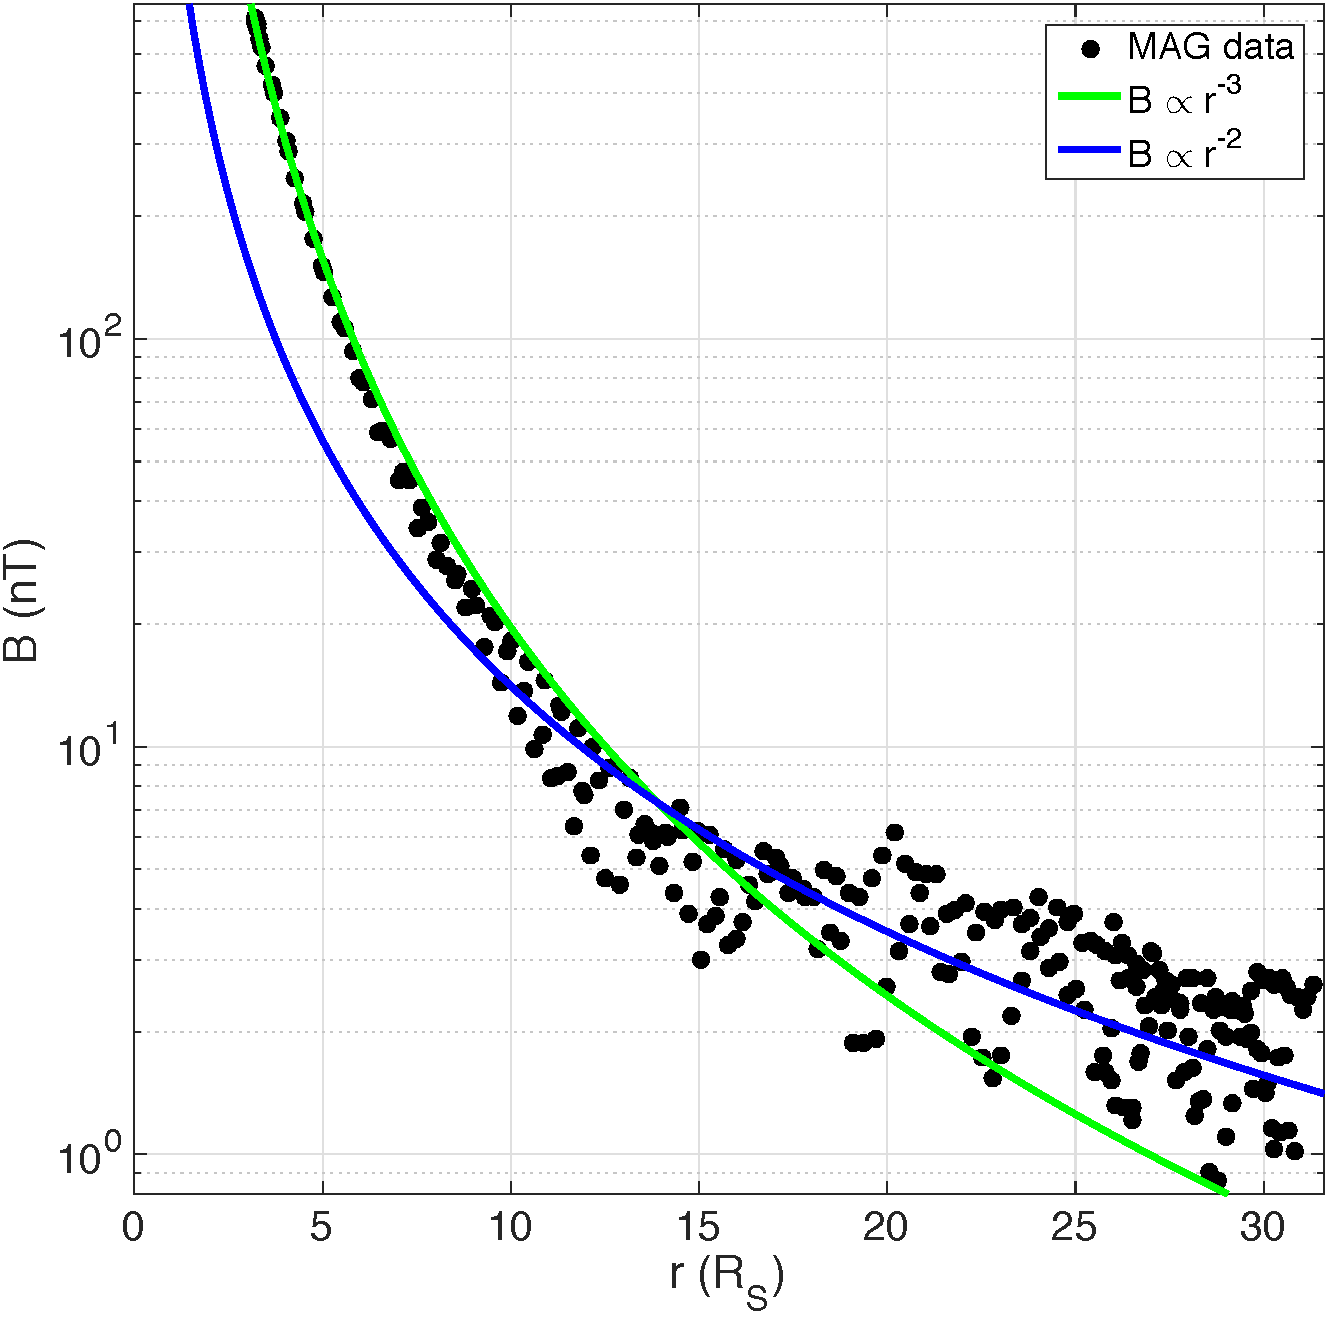
\includegraphics[width=0.6\textwidth]{compress/magdata.pdf}
\caption[Equatorial magnetic field data from \textit{Cassini} MAG.]{Total magnetic field strength $B$ against radial distance from planet center. Black circles are from \textit{Cassini} MAG data, measured on Saturn's dayside, taken from 3 equatorial orbits during Saturn equinox (Revs $120{\--}122$, 23~October to 17~December~2009). Example power law curves shown in green and blue for reference.}
\label{compress:fig:magdata}
\end{figure}

In Saturn's middle and outer magnetosphere, the  hot  ($>\SI{3}{keV}$) plasma population contributes more to the total plasma pressure than the colder equatorial plasma,  and values of plasma $\beta$ in the range ${\sim}2{\--}5$ have been observed  for this population in this region \citep{sergis2010}. This means that under some conditions the hot plasma population may control compressibility directly. The derivation of equation (\ref{compress:eq:key}) assumes the solar wind dynamic pressure is directly balanced by the magnetic pressure inside the magnetosphere; however, for $\beta > 1$ at the magnetopause boundary, the hot plasma pressure inside the magnetosphere is also significant in controlling pressure balance. Therefore $\alpha$ will be partially determined by how the hot plasma pressure $P_\mathrm{H}$ varies with radial distance (via the same arguments as laid out for equation (\ref{compress:eq:key}) above). \citet{gold1959} used the concept of magnetic flux tubes of plasma expanding isothermally to explain that, in a dipolar magnetic field, one would expect the hot plasma pressure to fall with radial distance according to $P_\mathrm{H} \propto r^{-4}$. We would thus expect $\alpha = 4$ for a fictitious magnetosphere where compressibility is dominantly controlled by a hot plasma population embedded in a dipole magnetic field, and a value even smaller for a magnetic field that varied more slowly than $r^{-3}$. We expand on this in Section~\ref{compress:sec:hotplasma}.

Jupiter's magnetosphere also has a significant internal plasma population, due to mass loading from the volcanic moon Io; the observed plasma $\beta$ associated with this population reaches 100 at \SI{45}{R_J} \citep{mauk2004}. The associated centrifugal force is also greater than the Saturnian parallel, mainly due to the larger overall size scale of Jupiter's magnetosphere, as discussed in Section~\ref{intro:sec:comparativemagnetospheres}. These conditions produce a more substantial disc-like magnetic field configuration at Jupiter, which significantly affects the magnetospheric compressibility; $\alpha$ has been measured empirically for this system as between ${\sim}4$ and ${\sim}5$ \citep{huddleston1998, joy2002, alexeev2005}. However these estimates are based on limited spacecraft observations and hence have large uncertainties associated with them.

Saturn's magnetosphere would therefore be expected to show compressibility behaviour that is intermediate between that of Jupiter ($\alpha \approx 4$) and the Earth ($\alpha \approx 6$). The inter-related factors of magnetic field structure, centrifugal force and plasma content that determine the overall stress balance may themselves show behaviour that varies with solar wind dynamic pressure (i.e. vary with size of the magnetosphere). It is therefore insightful to investigate Saturn's magnetospheric compressibility in response to changes in both external factors (the incident solar wind dynamic pressure) and internal factors (hot plasma content) in tandem.

\subsection{Models of Saturn's Magnetopause}\label{compress:sec:prevstudies}
\begin{table}
\caption[Estimates of magnetopause model parameters from previous studies.]{Estimates of magnetopause model parameters from previous studies.}\label{compress:table:prevstudies}
\centering
\begin{tabular}{c c c c}
\hline
Study & Size Range $(\si{R_S})$ & $a_1$ & $\alpha$   \\
\hline
{\citet{slavin1985}} & $< 19$ &  & $\sim 6.1$ \\
{\citet{hansen2005}}   & $21 - 28 $ &  & $\sim 5.2$ \\
{\citet{arridge2006}} & $17-29$ & $9.7 \pm 1.0 $ & $4.3 \pm 0.4$   \\
{\citet{kanani2010}} & $17-29$ & $10.3 \pm 1.7 $ & $5.0 \pm 0.8$ \\
{\citet{pilkington2015}} & $14 - 40$ & $10.8 - 16.5$ & $5.5 \pm 0.2$ \\
\hline
\end{tabular}
\end{table}
Previous studies have mostly employed \textit{in situ} magnetopause crossing data to create empirical models of the size and shape of Saturn's magnetosphere under different solar wind pressure conditions, in order to make estimates of $\alpha$ and $a_1$. \citet{slavin1985} used \textit{Pioneer} 11 and \textit{Voyager} 1 and 2 plasma and magnetometer data and modelled the magnetopause surface as a conic section. \citet{arridge2006} applied the formalism first described in \citet{shue1997} for the terrestrial system to Saturn using \textit{Cassini} MAG data, estimating the upstream solar wind pressure by assuming pressure balance with the magnetic pressure of the magnetosphere just inside the magnetopause. This model was then augmented by \citet{kanani2010} who used \textit{Cassini} plasma data in order to include thermal plasma pressure, as well as magnetic pressure, inside the magnetopause. Further improvements to the treatment of internal plasma pressure sources, and an extension of the crossing data set, were then made by \citet{pilkington2015}. Previous to these \textit{Cassini}-based studies, \citet{hansen2005} used a 3-D global magnetohydrodynamic simulation of Saturn's magnetosphere for the time period of \textit{Cassini}'s initial approach in order to investigate $\alpha$. The relevant parameters calculated in each study are shown in Table~\ref{compress:table:prevstudies}, where parameters relate to equation~\ref{compress:eq:key} with $R_\mathrm{MP}$ in units of $\si{R_S}$ and $D_{P}$ in nanopascals (\si{nPa}). In the study by \citet{pilkington2015}, they explain that their extended \textit{Cassini} data set includes more variable and high-$\beta$ crossings than previous studies. A k-means clustering algorithm was used to separate the crossing data set into three groups organized by local plasma $\beta$; while the estimates of $\alpha$ agreed in each group within the uncertainties, the estimates of $a_1$ did not, and showed a trend of increasing with larger average $\beta$, from ${\sim}10.8$ to ${\sim}16.5$.

The estimates of $a_1$ by \citet{arridge2006} and \citet{kanani2010} agree within the quoted uncertainties. In addition, in \citet{pilkington2015}, in order to account for the influence of local plasma $\beta$ on $a_1$, these authors repeat their analysis with a modification to equation~\ref{compress:eq:key} such that $D_\mathrm{P}$ is replaced by $D_\mathrm{P}/(1+\beta)$. With this adaptation, \citet{pilkington2015} measured $a_1 = 10.5 \pm 0.2$, which is consistent with previous results shown in Table~\ref{compress:table:prevstudies}. The estimates of $\alpha$ for each study agree at least within 2$\sigma$ uncertainty level, where appropriate, and in general are consistent with the picture of a magnetosphere that behaves intermediately between the rigid Earth case and the more compressible Jupiter case. However the role of the global hot plasma content in controlling magnetospheric compressibility is still not fully understood.

The current lack of multi-point simultaneous observations in Saturn's magnetosphere mean that the use of \textit{in situ} data is inherently limited, as the large scale structure of the magnetosphere at the exact time corresponding to one magnetopause crossing cannot be readily obtained. This makes it difficult to interpret the global physical processes that are controlling the compressibility behaviour. Instead empirical studies, such as those referred to above, provide an `average' picture of the magnetopause morphology over varying internal and external conditions. In addition, the empirical studies discussed must assume that the magnetopause is in dynamical equilibrium at the time of crossing observations (i.e. it is not accelerating) in order to estimate the solar wind pressure via Newtonian pressure balance, which is almost never the case at Saturn \cite[e.g.][]{dougherty2005,masters2011,pilkington2015}.

In this study we adopt a more theoretical approach, in order to complement these previous observational studies. The 2-D axisymmetric force-balance model of Saturn's dayside magnetosphere, first presented by \citet{achilleos2010a} and described in Chapter~\ref{chap:intro}, is used to investigate magnetospheric compressibility. This model can be calculated at a chosen range of magnetopause radii. The corresponding estimated upstream solar wind pressure can be readily obtained using calculated plasma and magnetic field information just inside the magnetopause boundary and assuming pressure balance across the magnetopause, which is static in this model. These theoretical estimates of $D_\mathrm{P}$ can then be used to make estimates of $\alpha$ and $a_1$. In addition, \citet{achilleos2010a} referred to a `hot plasma index' in the model, with which the hot plasma content in the magnetosphere can be parameterised. We revisit this concept herein, in order to investigate the influence of the global hot plasma population on magnetospheric compressibility.

\section{Method}\label{compress:sec:method}
\subsection{Magnetodisc Model Calculations}\label{compress:sec:model}
In this study we use the model for Saturn's magnetodisc originally set out in \citet{achilleos2010a}, and described in detail in Section~\ref{intro:sec:forcebalancemodel} of this thesis. As a reminder, the model is axisymmetric about the planetary dipole/rotation axis, which are assumed to be aligned, and is constructed based on the assumption of force balance in the rotating plasma of the magnetosphere such that 
\begin{equation}\label{compress:eq:forcebalance}
\boldsymbol{J} \times \boldsymbol{B} = \nabla P - nm_i\omega^2\rho\boldsymbol{e}_\rho
\end{equation}
where $\boldsymbol{J}$ is the current density, $\boldsymbol{B}$ is the magnetic field vector and $\rho$ is cylindrical radial distance from the axis, with $\boldsymbol{e}_\rho$ its unit vector. The plasma properties are isotropic pressure $P$, ion number density $n$, mean ion mass $m_i$ and angular velocity $\omega$. The model assumes the magnetospheric plasma comprises a cold population with pressure $P_\mathrm{C}$, confined towards the rotational equatorial plane due to the centrifugal force exerted on it, and a hot population with associated plasma pressure $P_\mathrm{H}$ constant along magnetic field lines. 

For the cold plasma population, the pressure is constrained by equatorial radial profiles of plasma properties, obtained from studies using the \textit{Cassini} CAPS and MIMI instruments, as summarised in \citet{achilleos2010a,achilleos2010b}. For  the hot plasma population, the pressure $P_\mathrm{H}$ may be completely characterized by a particular equatorial plasma pressure $P_\mathrm{H0}$, and flux tube volume $V$ per unit of magnetic flux, where
\begin{equation}\label{compress:eq:ftv}
V = \int_{0}^{s_{B}} ds/B, 
\end{equation}
and $ds$ is an element of arc length along the magnetic field line. The integral limits represent measurement along a field line of total length $s_B$ between the southern and northern ionospheric footprints at $\SI{1}{R_S}$. The flux tube volume is therefore dependent on both the shape of magnetic field lines, via $ds$, and the strength of the field, via $B$. 

\citet{achilleos2010a} combined quantile fits of equatorial profiles of equatorial hot plasma pressure \citet{sergis2007} with a radial profile of $V$ obtained from an empirical magnetic field model \citep{bunce2007} in order to show a picture of a highly variable hot plasma population, that follows neither adiabatic ($P_\mathrm{H0}V^{5/3} =$ constant) nor isothermal ($P_\mathrm{H0}V =$ constant) transport behaviour. In light of these observations, the original \citet{achilleos2010a} model simply parameterised the global hot plasma content by a single `hot plasma index' $K_\mathrm{H}$, where $ K_\mathrm{H}= P_\mathrm{H0}V$ is constant beyond $\SI{8}{R_S}$, and $P_\mathrm{H0}$ decreases linearly to zero inside that distance. A similar parameterisation, though with different values of the constants, was made in \citet{caudal1986}, who argued that for the Jovian system, under the expected conditions of rapid radial diffusion, the hot plasma would be transported isothermally. Parameterising the hot plasma content in this way provides the flexibility to very simply characterize the level of ring current activity in the model, and thus investigate the effect of the hot plasma content on magnetospheric compressibility. We recognize that more detailed studies of hot plasma dynamics may require investigation of different parameterisations in the future. In particular, a more physically realistic hot plasma profile was developed in \citet{achilleos2010b}, however the use of such a profile does not affect the basic conclusions of this study.

In this study a value of $K_\mathrm{H}=\SI{1e6}{Pa m T^{-1}}$ was initially adopted to parameterise the ring current activity in the magnetosphere, representing broadly `average' conditions, corresponding to the median quantile fit of the hot plasma pressure from \citet{sergis2007}. The magnetodisc model was then calculated at 30 different magnetopause radii $R_\mathrm{MP}$, equally spaced over a range of $14{\--}\SI{40}{R_S}$, in order to match the range in this parameter observed in the data set presented by \citet{pilkington2015}. For each calculation, the corresponding solar wind dynamic pressure incident on the magnetopause nose was estimated from model magnetospheric parameters by assuming pressure balance across the model magnetopause boundary. Specifically, we used the relationship given in equation~\ref{compress:eq:forcebalance}, with $P_{\mathrm{MS}}=P_\mathrm{H}+P_\mathrm{C}$, extracting values for $B_\mathrm{MS}$, $P_\mathrm{H}$ and $P_\mathrm{C}$ from the model just inside the magnetopause boundary at the equator. For $k$, we used a value of 0.881, as this is appropriate for high ($\gtrsim 8$) Mach number flow with $\gamma = 5/3$  \citep{spreiter1966}, which is valid for the solar wind at Saturn's orbit \cite[e.g.][]{slavin1985,achilleos2006}. However as it is of order unity it does not significantly affect our estimates of $D_\mathrm{P}$ or the conclusions of this study. This value of $k$ is also used in the previous studies discussed in Section~\ref{compress:sec:prevstudies}.

A profile of $R_\mathrm{MP}$ versus $D_\mathrm{P}$ for a given $K_\mathrm{H}$ value was then constructed in order to estimate the model compressibility parameter $\alpha$. The value of $K_\mathrm{H}$ in the model was then varied linearly over the range $10^5{\--}10^7~\si{Pa m T^{-1}}$, in accordance with aforementioned  observations, and the effect on magnetospheric compressibility was investigated. 


\subsection{Fitting Procedure and Error Estimation to Calculate $\alpha$}
We made estimates of the compressibility parameter $\alpha$ for each profile of $R_\mathrm{MP}$ and $D_\mathrm{P}$ simulated data points using linear least squares regression analysis as follows. If we have a set of $n$ data points $\{x_i,y_i\}$ that we have reason to believe are linearly dependent, we can attempt to find a `best fit line' to describe this relationship, $\hat{y}(x) = mx + b$. In our study, this corresponds to the logarithm of equation~\ref{compress:eq:key},
\begin{equation}
\log{R_\mathrm{MP}}{=}-1/{\alpha}\log {D_\mathrm{P}}+\log{a_1},
\end{equation}
such that $\hat{y} = \log{R_\mathrm{MP}}$, $x =\log{D_\mathrm{P}}$, $ m = -1/\alpha$ and $b = \log{a_1}$. We can then obtain estimates of parameters $a_1$ and $\alpha$ by fitting the logarithms of our simulated data set, $\{x_i=\log{D_\mathrm{P}}$, $y_i=\log{R_\mathrm{MP}}\}$ with a best fit line, and estimating $m$ and $b$.

In order to obtain estimates of the parameters $m$ and $b$, we minimize the sum of the squares of the residuals between the data and the best fit line points,
\begin{equation}
SS = \sum\limits_{i=1}^{n}(y_i-\hat{y_i})^2,
\end{equation}
with respect to $m$ and $b$. This yields the solutions
\begin{align}
 m  &=  \frac{\sum(x_i-\bar{x})(y_i-\bar{y})}{\sum(x_i-\bar{x})^2}  \nonumber\\ 
 b & =   \bar{y} - m\bar{x} 
\end{align}
where $\bar{x}$ denotes the mean of all $x_i$, and similarly for $\bar{y}$, and all summations are calculated over all $n$ data points. This technique assumes the errors associated with the data are uniform such that all $\{x_i,y_i\}$ are weighted equally, and is known as the ordinary least-squares solution. The approximate standard errors of the parameters, $s_m$ and $s_b$, are then given by
\begin{align}
s_m^2 = & \frac{\hat{\sigma}^2}{\sum(x_i-\bar{x})^2}\nonumber\\
\nonumber\\
s_b^2 = & \frac{\hat{\sigma}^2\sum x_i^2}{n\sum(x_i-\bar{x})^2}
\end{align}
where $\hat{\sigma}^2 = SS/(n-2)$ is the estimated variance in the simulated `measurements', and $(n-2)$ is the number of degrees of freedom. $s_m$ and $s_b$ are estimates of the changes in $m$ and $b$ that correspond to changes of order $\hat{\sigma}^2$ in $y_i$. These estimates require that the parameters $m$ and $b$ are uncorrelated, which is a valid assumption over ranges in magnetospheric size where both $m$ and $b$ are approximately constant. These results are derived from matrix relations that are generalized for fittings with greater than two parameters; more information can be found in \citet{yang2005}.

The corresponding errors in the parameters $a_1$ and $\alpha$ are then calculated using standard error propagation given the relationship between them and $m$ and $b$ respectively; for a variable $u = u(v)$, the error in $u$, $\sigma_u$, is given by
\begin{equation}
\left|\frac{du}{dv}\right|\sigma_v.
\end{equation} 

\section{Results and Discussion}\label{compress:sec:results}
\subsection{Magnetospheric Compressibility with `Average' Hot Plasma Conditions}
\begin{figure}
\centering
\noindent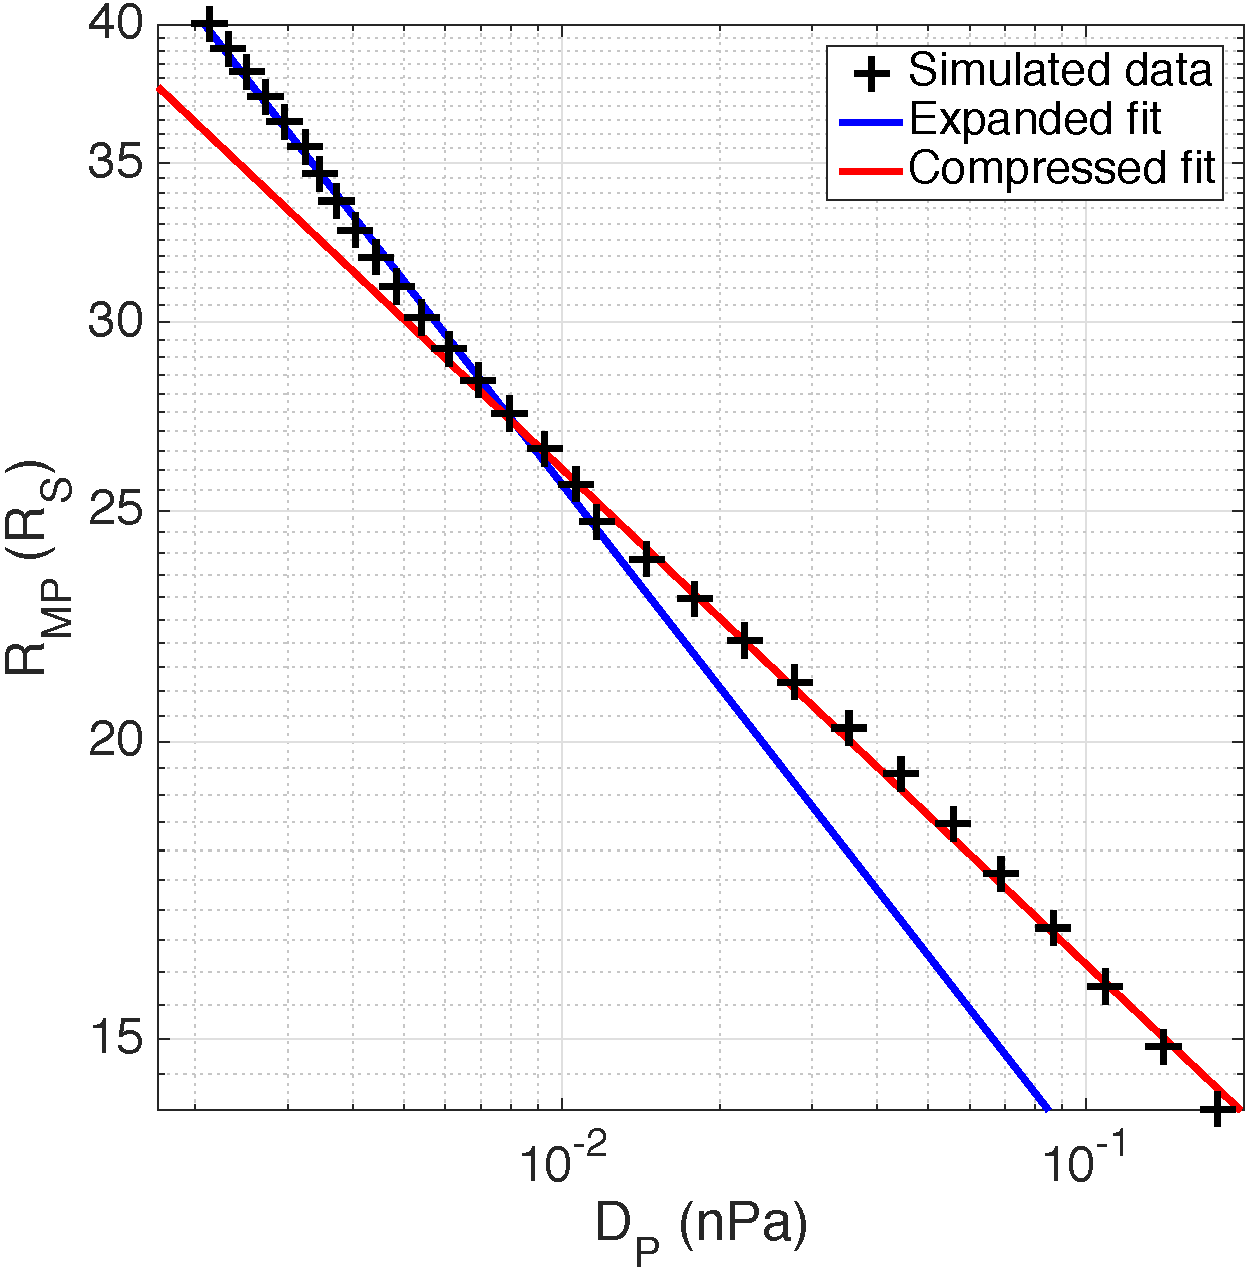
\includegraphics[width=0.6\textwidth]{compress/moneyplot.pdf}
\caption[Magnetopause radius versus solar wind dynamic pressure compressibility profile for `typical' hot plasma content $K_\mathrm{H}$.]{Magnetopause radius $R_\mathrm{MP}$ as a function of solar wind dynamic pressure $D_{P}$, on a logarithmic scale, for $K_\mathrm{H}=\SI{1e6}{Pa m T^{-1}}$. Each black cross represents the result of one model calculation. The linear least squares regression line fitted to calculations with $R_\mathrm{MP} \leq \SI{25}{R_S}$ is shown in red, and for calculations with $R_\mathrm{MP} > \SI{25}{R_S}$ shown in blue.}
\label{compress:fig:money1}
\end{figure}
Figure~\ref{compress:fig:money1} shows the magnetopause radius $R_\mathrm{MP}$ for each model calculation as a function of the corresponding solar wind dynamic pressure, calculated as described in Section~\ref{compress:sec:pressurebalance}, on a logarithmic scale, with $K_\mathrm{H}=\SI{1e6}{Pa m T^{-1}}$. Linear least squares regression lines have been fitted to two regions of the data as described in the caption.

On such a plot, data that exactly obey equation (\ref{compress:eq:key}) with constant $a_1$ and $\alpha$ would follow a straight line with slope $-1/\alpha$ and y-intercept $a_1$. However it can clearly be seen that for this simulated `data set', neither $a_1$ nor $\alpha$ are constant with system size.
In particular, a distinct shift in behaviour can be identified at $R_\mathrm{MP} \approx \SI{25}{R_S}$. We therefore divided the simulated data set into two groups, $R_\mathrm{MP} \leq \SI{25}{R_S}$, which we shall refer to as the compressed regime, and $R_\mathrm{MP} > \SI{25}{R_S}$, which we shall refer to as the expanded regime. We then fit each data group with a linear least squares regression line separately, in order to make estimates of relevant parameters and investigate how they differ as the system expands. It should be noted that the value of $\SI{25}{R_S}$ in particular was selected by eye, and a value up to ${\sim}\SI{28}{R_S}$ could be chosen to divide the two regimes, and does not significantly affect our conclusions.

\begin{table}
\caption[Estimates of compressibility parameters for this study.]{Estimates of compressibility parameters calculated from the model outputs shown in Figure \ref{compress:fig:money1}.}\label{compress:table:money1}
\centering
\begin{tabular}{c c c c}
\hline
Regime & Size Range $(\si{R_S})$ & $a_1$ & $\alpha$   \\
\hline
Compressed & $14 - 25 $ & $10.0 \pm 0.1  $ & $4.80 \pm 0.09$ \\
Expanded & $25 - 40 $ & $7.0 \pm 0.2$ & $3.53 \pm 0.06$ \\
\hline
\end{tabular}
\end{table}
The estimates for $\alpha$ and $a_1$ with standard error uncertainties, for the two regimes, are shown in Table~\ref{compress:table:money1}. The full fitting procedure and calculation of uncertainties are described in the Appendix. It should be noted that such uncertainties should be taken as a guideline only. We do not suggest that the data exactly follow this underlying distribution, and have made this simplification to give an overall picture of the behaviour, given the limitations of our simulated data set. Real observational data would of course be subject to significant measurement errors, and the resulting parameter uncertainties would be higher than those we have calculated for our simulations.

For the compressed regime, the estimates of $a_1$ and $\alpha$ are broadly consistent with the previous results shown in Table~\ref{compress:table:prevstudies} at the 2$\sigma$ level, except the $\alpha$ estimate of \citet{pilkington2015}. For the expanded regime, the estimated values are both significantly smaller than those calculated in any previous studies. The value of $\alpha = 3.53$ in particular corresponds to the magnetosphere becoming more sensitive to changes in solar wind pressure as it expands, and in fact becoming marginally more compressible than the Jovian system, indicated by the value of $\alpha < 4$ (see discussion in Section~\ref{compress:sec:prevstudies}).This implies that under appropriate conditions, the compressibility behaviour of the Jovian magnetosphere may actually be an intermediate between Earth and Saturn. This is investigated in more detail later in Section \ref{compress:sec:jup}.

It was shown in \citet{achilleos2008}, who studied the long term behaviour of the size of Saturn's magnetosphere as measured by \textit{Cassini}, that the magnetopause radius is well described by a bimodal probability distribution, with local maxima at $22 \pm \SI{1.5}{R_S}$ and $27 \pm \SI{1.3}{R_S}$ (apparently distinct from the typical distributions of the solar wind dynamic pressure). In the earlier empirical studies, the magnetosphere is more often observed in a compressed regime, as shown by the observed ranges in Table~\ref{compress:table:prevstudies}, due to the more restricted data sets available for use in those studies, and the higher average solar activity at the time of observations \cite[e.g.][]{hathaway2015}. Thus the corresponding estimates of $a_1$ and $\alpha$ are likely to be weighted more towards values typical of such conditions. We also find that our parameter estimates are very sensitive to the choice of hot plasma index $K_\mathrm{H}$, which may be a cause of the discrepancy between our results and previous studies. We shall investigate this aspect in depth in the following sections, but first we will look at which components of the internal structure contribute most to the formation of this `knee' in compressibility behaviour at ${\sim}\SI{25}{R_S}$, as seen in Figure~\ref{compress:fig:money1}.

Figure~\ref{compress:fig:pcomps} shows the individual contributions from the hot, cold and magnetic pressure components to the total magnetospheric pressure just inside the model's magnetopause boundary. It can clearly be seen that the magnetic pressure, $P_\mathrm{B}=B^2/2\mu_0$, is the dominant component for all system sizes. Values of plasma $\beta$ have been extracted for the hot and cold plasma populations separately, and the hot plasma beta $\beta_\mathrm{H}$ and cold plasma beta $\beta_\mathrm{C}$ are both $\lesssim 0.7$ across all system sizes, while the total plasma $\beta$ of the collective plasma surpasses unity for the largest system sizes, where $R_\mathrm{MP} \gtrsim \SI{30}{R_S}$. The hot and cold pressure components are comparable for $R_\mathrm{MP} \gtrsim \SI{25}{R_S}$, below which the cold pressure dominates. 
\begin{figure}
\centering
\noindent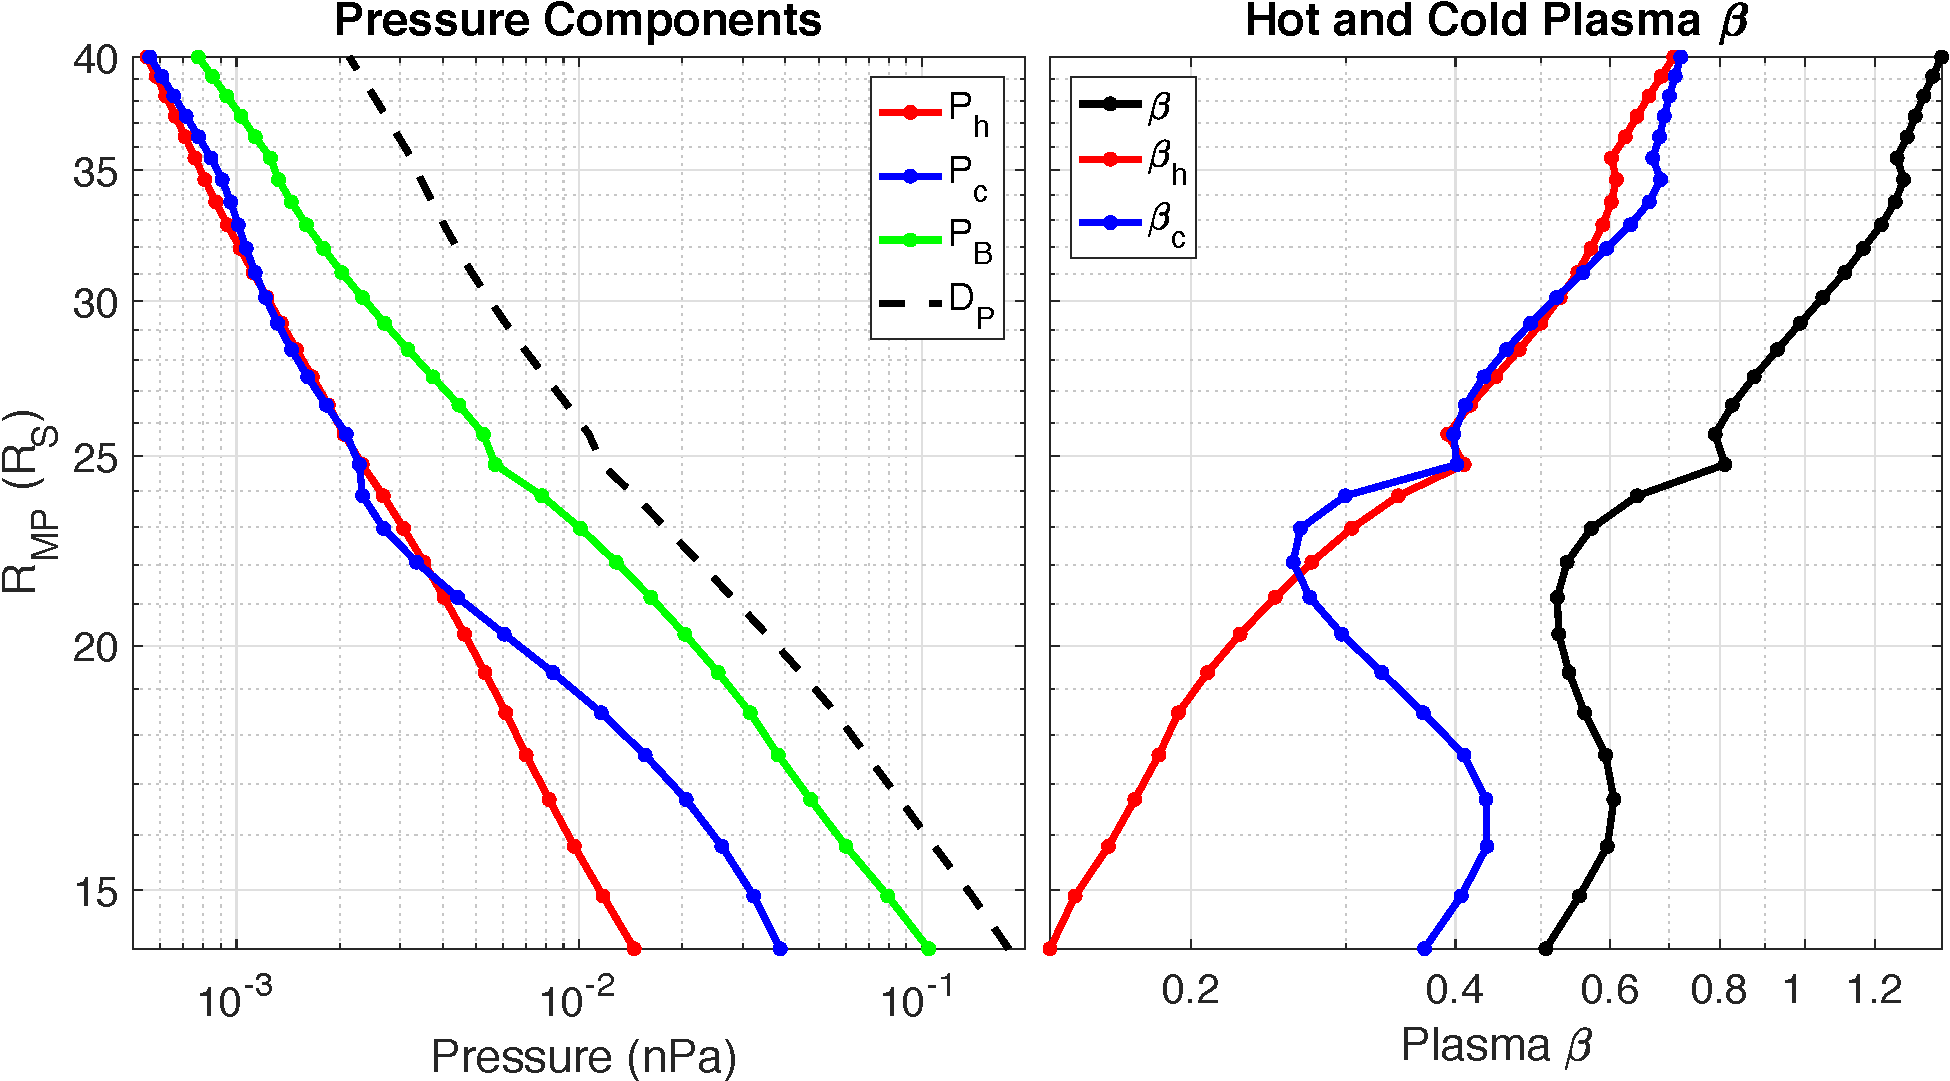
\includegraphics[width=\textwidth]{compress/pcomps.pdf}
\caption[Pressure components and plasma $\beta$ just inside the magnetopause boundary for typical $K_\mathrm{H}$.]{The individual contributions to the total magnetospheric pressure just inside the magnetopause boundary for different system sizes, corresponding to results in Figure~\ref{compress:fig:money1}. (left panel) The hot plasma, cold plasma and magnetic pressure components are shown in red, blue and green respectively, with the total pressure divided by $k=0.881$, i.e. the corresponding solar wind dynamic pressure, shown as a black dashed line for comparison. (right panel) The values of plasma $\beta$ just inside the magnetopause boundary for the collective plasma (black), and for each of the hot (red) and cold (blue) plasma populations separately.}
\label{compress:fig:pcomps}
\end{figure}
 
The magnetic pressure profile in particular appears to exhibit a change in gradient around $\SI{25}{R_S}$ similar to the solar wind pressure profile, and indeed has a measured gradient changing from $-1/(4.9 \pm 0.3)$ for the compressed regime to $ -1/(4.2 \pm 0.2)$ for the expanded regime, with gradients fitted using the same method as for the $D_\mathrm{P}$ profile. These values do not agree exactly with those found for the $D_\mathrm{P}$ profile regions (see Table~\ref{compress:table:money1}) due to the minor influence of the plasma pressures, particularly for the expanded regime. However the magnetic pressure profile shows the same overall trend, and thus suggests that how magnetic pressure varies with system size is a dominant factor in controlling the change in compressibility behaviour.
 
As discussed in Section~\ref{compress:sec:intro}, the magnetic field strength (and therefore magnetic pressure) varies more slowly with radial distance for a more disc-like magnetic field structure, i.e. the index $\chi$ in $B \propto r^{-\chi}$ is smaller than the dipole value. This corresponds to a steeper gradient of the $R_\mathrm{MP}$ versus magnetic pressure profile on a logarithmic scale, as the gradient of such a profile is $-1/2\chi$. Therefore the observed behaviour of the magnetic pressure profile can be interpreted as the formation of a magnetodisc structure in the magnetosphere, but more so for the more expanded regime. This can be understood theoretically as follows. The magnetodisc forms due to the magnetic tension force increasing, in order to balance the centrifugal force exerted outwards on the subcorotating cold plasma in the magnetosphere. This tension force is proportional to $B^2/r_c$, where $r_c$ is the radius of curvature of the magnetic field lines, and therefore can be increased by a larger magnetic field strength or a smaller radius of curvature. For the compressed regime, $B$ in the outer magnetosphere is still comparatively large and so can maintain a sufficient tension force for a relatively large $r_c$. For the more expanded regime, as $B$ generally decreases, the radius of curvature must also decrease in order to maintain a sufficient tension force, corresponding to the formation of a disc structure. This was also observed empirically by \citet{arridge2008}, who employed \textit{Cassini} MAG data to demonstrate that under strong solar wind pressure conditions, when the magnetosphere was compressed to $R_\mathrm{MP} < \SI{23}{R_S}$, the disc structure was effectively destroyed on the dayside, and the magnetic field became quasi-dipolar.

A study by \citet{bunce2007} used \textit{Cassini} MAG data to construct an empirical model of the ring current in Saturn's middle magnetosphere, and used the calculated magnetic fields to estimate the corresponding solar wind dynamic pressures in order to investigate magnetospheric compressibility, similar to our study. They also found a value of $\alpha$ that decreased with system size, over a range of $R_\mathrm{MP} = 16{\--}\SI{30}{R_S}$, with overall results in agreement with \citet{arridge2006}. They explained this in terms of an increase in the ring current magnetic moment for an expanded magnetosphere, which corresponds to an enhancement in the magnetodisc structure. Our preliminary results are therefore in general agreement with this previous study, which suggests that the magnetospheric compressibility is primarily controlled by how the magnetic pressure at the magnetopause boundary varies with system size. However it is worth noting that the model used by \citet{bunce2007} assumes a ring current density that falls with cylindrical radial distance as $1/\rho$; this is not the case in this study, as the \citet{achilleos2010a} model calculates azimuthal current profiles directly from the source function $g$ described in Section~\ref{compress:sec:model} \cite[see][]{caudal1986, achilleos2010a}.

Thus far we have neglected to include the `pressure' contribution of the centrifugal force exerted on the magnetopause boundary surface, and whether this has a role in controlling magnetospheric compressibility. The centrifugal force per unit volume at the magnetopause boundary is given by $F_c = nm_i\rho\omega^2$ (see equation~\ref{compress:eq:forcebalance}). \citet{pilkington2014} explained that, by making the assumption that the magnetopause current layer has a comparable density and rotation rate to the plasma just inside the boundary, we can estimate the corresponding pressure contribution by simply multiplying this volume force by the thickness of the magnetopause current layer. By approximating the current layer thickness as $\SI{1}{R_S}$, following \citet{masters2011}, we find that across all system sizes, the centrifugal term is around an order of magnitude smaller than any other pressure component, and therefore is not investigated further in this study.

\subsection{Influence of Hot Plasma Content} \label{compress:sec:hotplasma}
The procedure leading to the results shown in Figure \ref{compress:fig:money1}, described above, was then repeated using 20 different values of the hot plasma index $K_\mathrm{H}$, equally spaced in the range $10^5 {\--} 10^7~\si{Pa m T^{-1}}$, and calculating the model at 20 different sizes in the range $R_\mathrm{MP} = 14{\--}\SI{40}{R_S}$ for each of these $K_\mathrm{H}$ values. The results are plotted in Figure \ref{compress:fig:money2}, which shows how magnetopause radius varies with solar wind dynamic pressure on a logarithmic scale, as for Figure \ref{compress:fig:money1}, with the hot plasma index used in the model represented by the colour.
\begin{figure}
\centering
\noindent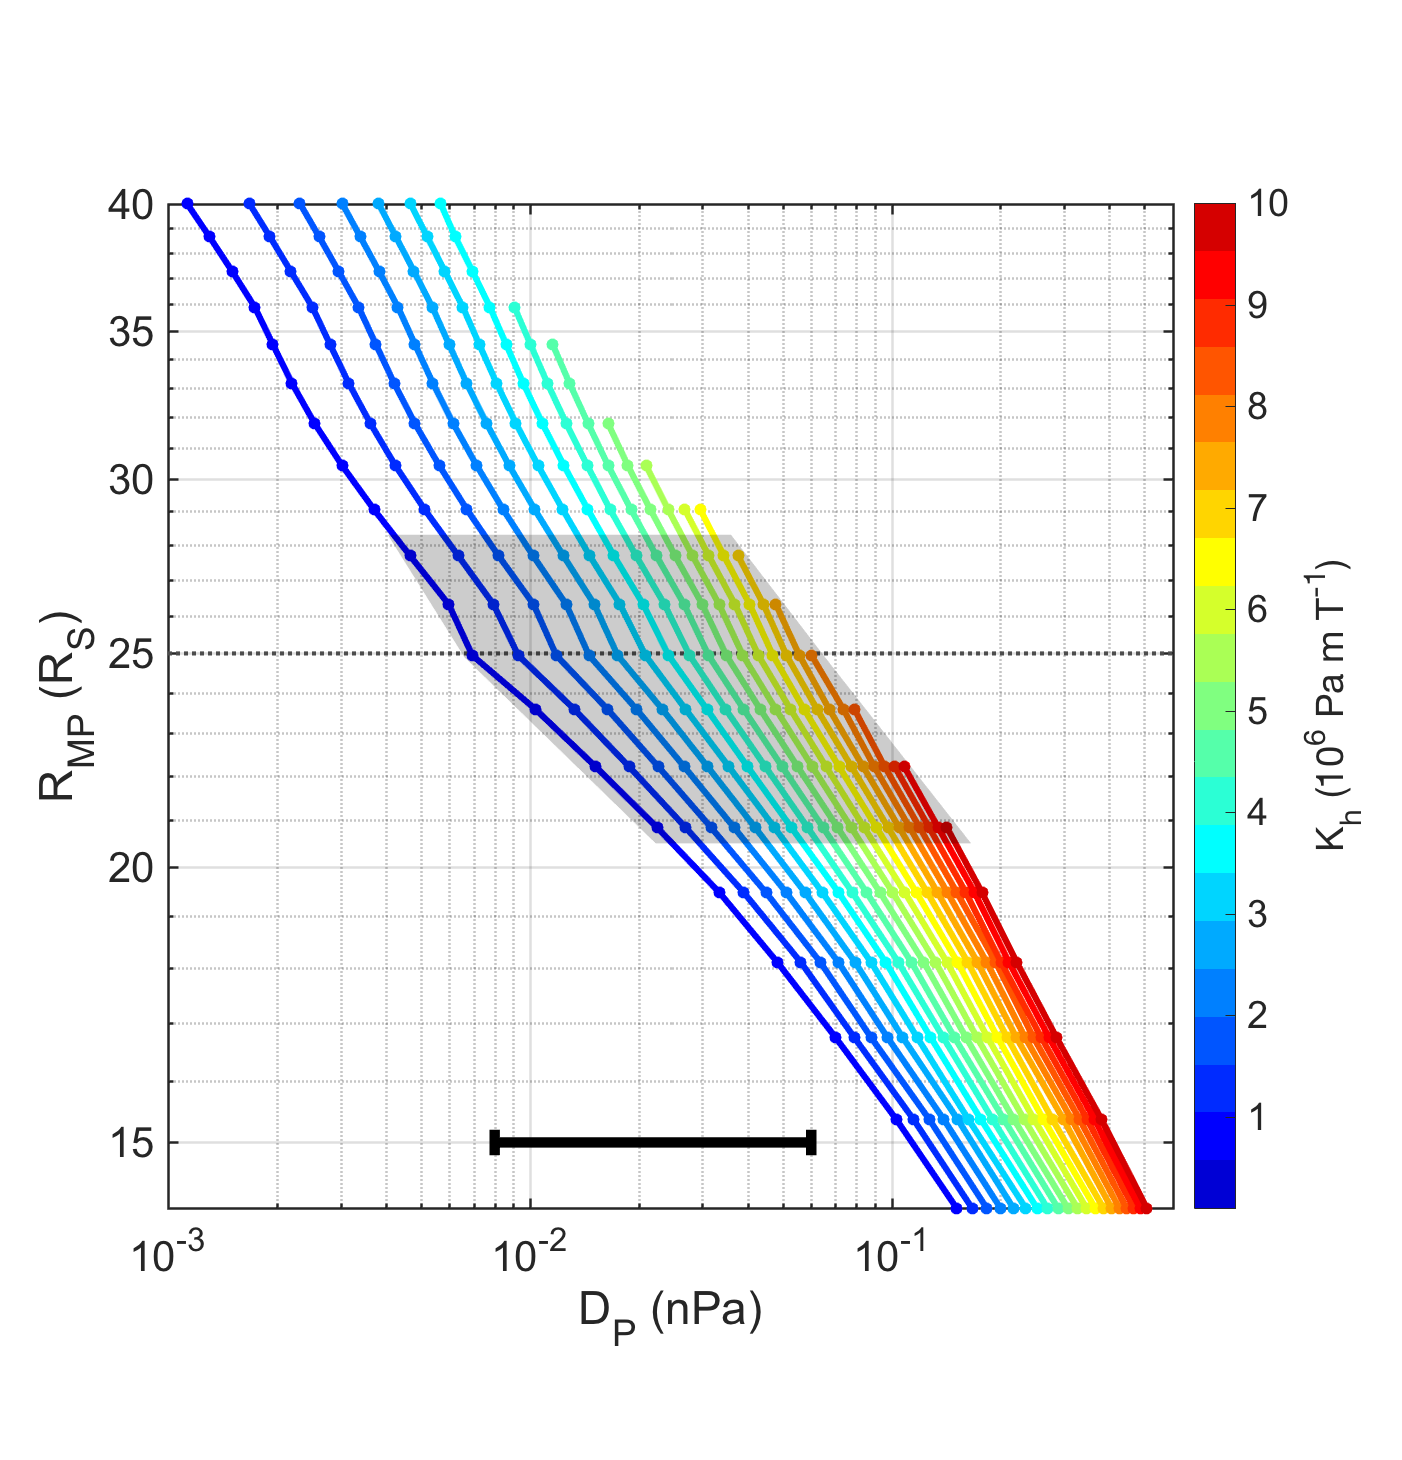
\includegraphics[width=0.8\textwidth]{compress/money2.pdf}
\caption[Magnetopause radius versus solar wind dynamic pressure compressibility profiles for a range of $K_\mathrm{H}$.]{Magnetopause radius $R_\mathrm{MP}$ as a function of solar wind dynamic pressure $D_\mathrm{P}$, on a logarithmic scale, for different $K_\mathrm{H}$ values as shown by the colour bar. Each solid dot represents the result of one model calculation. A dashed line at $R_\mathrm{MP}{=}\SI{25}{R_S}$ is shown for reference. The grey shaded region highlights data points with $R_\mathrm{MP}$ in the range $20.5{\--}\SI{28.3}{R_S}$, corresponding to expected values at Saturn according to empirical observations by \citet{achilleos2008}. The black horizontal bar shows the approximate range of $D_\mathrm{P}$ typically observed at Saturn ($0.008 {\--} \SI{0.06}{nPa}$) according to \textit{Cassini} CAPS solar wind data, also from \citet{achilleos2008}. However it should be noted that values of $D_\mathrm{P}$ in the full range shown in this figure ($0.001 {\--} \SI{0.5}{nPa}$) have been observed empirically.} 
\label{compress:fig:money2}
\end{figure}
 
For sufficiently high values of the hot plasma index, the model calculation would not converge to the prescribed 0.5$\%$ tolerance for large magnetopause radii, hence the lack of coverage in this region of parameter space. We attempted to mitigate this by, at each iteration, weighting the previous Euler potential solution $\alpha_{i-1}(r,\mu)$ up to 10 times more heavily than $\alpha_{i}(r,\mu)$ (see Section \ref{intro:sec:forcebalancemodel}), such that it would approach a convergent solution more slowly. However the correspondingly more stringent tolerance required in this case was still not achieved. The reason for this lack of convergence is that in such circumstances an equilibrium force-balance solution cannot be found, for a field structure that can contain such a level of simulated hot plasma. It is interesting to note that this only occurs under physical conditions we would not expect to typically observe the magnetosphere; for typical values of hot plasma content and solar wind dynamic pressure observed at Saturn, the model calculations are well within the convergence limit, as shown by the black horizontal bar in Figure \ref{compress:fig:money2}.

The most obvious feature apparent in Figure~\ref{compress:fig:money2} is the effect of the hot plasma content on the parameter $a_1$, reflected in the shift of the y-intercept for different compressibility profiles. Estimates of this parameter vary from $10.1 \pm 0.2$ for $K_\mathrm{H}=\SI{1e5}{Pa m T^{-1}}$ to $11.3 \pm 0.03$ for $K_\mathrm{H}=\SI{1e7}{Pa m T^{-1}}$, measured by applying a linear least squares regression line to the entire profile for each $K_\mathrm{H}$ value. This is comparable to the behaviour observed empirically by \citet{pilkington2015} (discussed in Section~\ref{compress:sec:prevstudies}), who calculated that their estimates of $a_1$ varied from ${\sim}11$ for the data set grouped by low average plasma $\beta$ ($\beta\lesssim 1$), to ${\sim}16$ for the data set with high average $\beta$ ($\beta\gtrsim 10$). However it should be noted that, while positively correlated, global hot plasma content $K_\mathrm{H}$ and local plasma $\beta$ are not interchangeable concepts, and have a relationship that is dependent on magnetosphere size, as discussed in detail later. 

These observations of variable $a_1$ correspond to the magnetosphere being observed in a range of sizes for fixed solar wind dynamic pressure, up to $10{\--}\SI{15}{R_S}$ in both \citet{pilkington2015} and this study. \citet{pilkington2015} interpreted this observation theoretically as the magnetosphere existing in either a plasma-depleted or plasma-loaded state, transitioning between these states perhaps via Vasyliunas-style reconnection and associated ejection of plasmoids \citep{vasyliunas1983}, or interchange events \citep{mitchell2015}. If we assume that such transitions can occur at least to some degree independently of the incident solar wind dynamic pressure, then it seems intuitive that there should exist a range of possible system sizes for a fixed $D_\mathrm{P}$, but different $K_\mathrm{H}$. 

This can be explained as follows. Consider a magnetopause initially in dynamic equilibrium with the upstream solar wind dynamic pressure, and what happens when the plasma pressure inside the magnetopause boundary drops due to some plasma loss process. The pressure across the boundary is now unbalanced, with the incident $D_\mathrm{P}$ greater than the total plasma and magnetic pressure inside the magnetosphere. The magnetopause location therefore moves inwards and the magnetosphere is compressed, causing an enhancement in the magnetic field strength $B$. The magnetic pressure therefore increases inside the magnetopause boundary, until pressure balance is restored and a new equilibrium magnetopause location is found. We would also expect the remaining magnetospheric plasma pressure to in general increase as the magnetopause moves inwards. This scenario thus corresponds to the magnetosphere generally being observed at a smaller size when the plasma content or pressure is lower, resulting in a lower estimate for the parameter $a_1$.

The variation in compressibility behaviour with varying system size and hot plasma content shown in Figure~\ref{compress:fig:money2} is less intuitive. As with our initial results, there appears to be a shift in behaviour at around $\SI{25}{R_S}$ for all profiles, although becoming less pronounced as $K_\mathrm{H}$ increases. Therefore for each individual profile at a given $K_\mathrm{H}$ value, the simulated data were again divided into two groups, a compressed regime and an expanded regime, separated at $\SI{25}{R_S}$, and we applied linear fits to these regions separately to make estimates of $\alpha$. The resulting estimates are shown in Figure~\ref{compress:fig:alphas}. Groups with fewer than three individual data points were not fit, hence for the expanded regime the estimates do not cover the full range of $K_\mathrm{H}$.
\begin{figure}
\centering
\noindent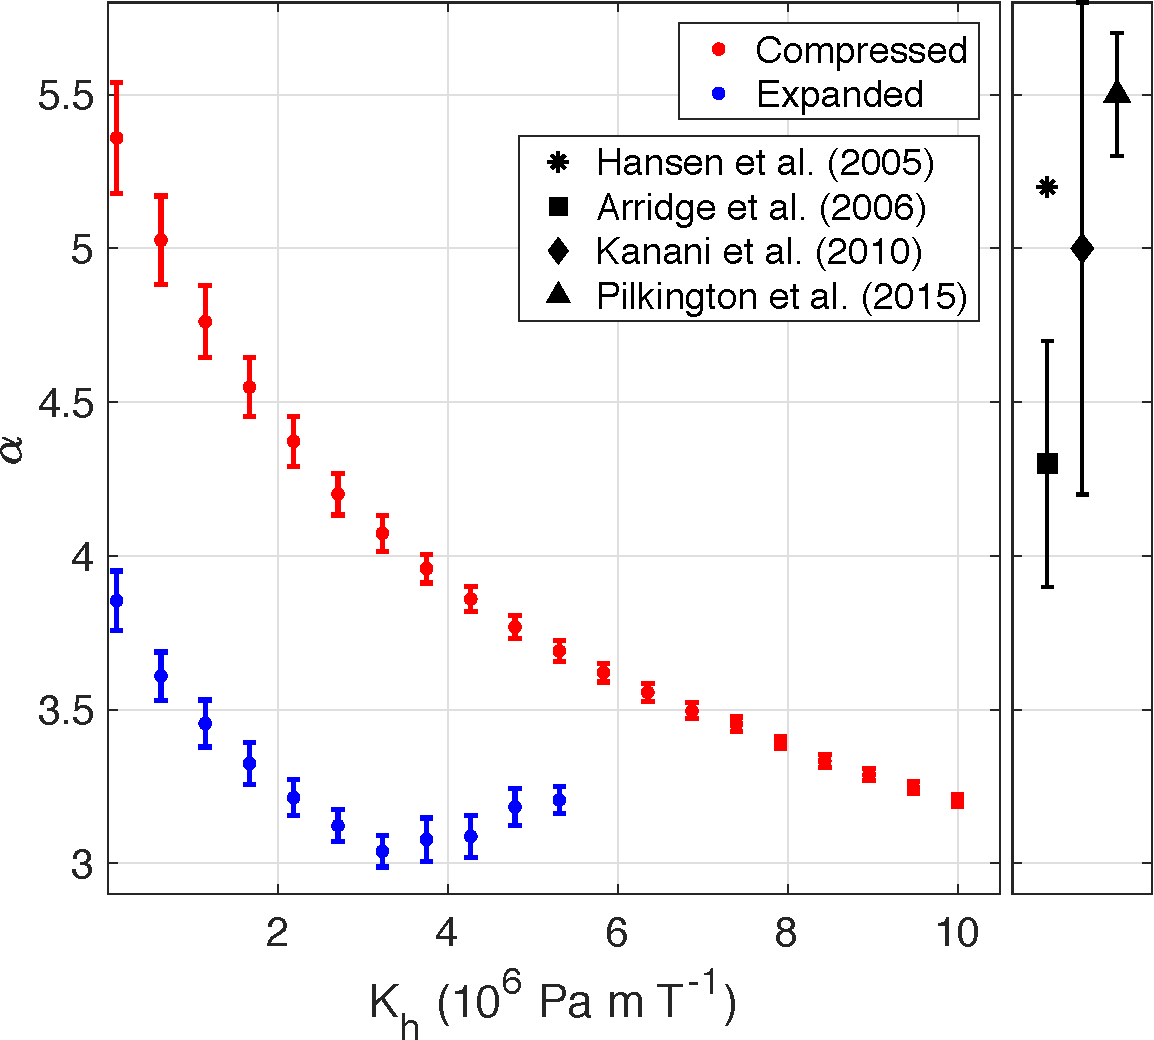
\includegraphics[width=0.8\textwidth]{compress/alphas.pdf}
\caption[Estimates of magnetospheric compressibility parameter $\alpha$, for different system sizes and $K_\mathrm{H}$ values.]{Left panel: estimates in the compressibility parameter $\alpha$, as a function of hot plasma index $K_\mathrm{H}$. Estimates made using the compressed regime profiles ($R_\mathrm{MP} \leq \SI{25}{R_S}$) are shown in red, and those for expanded regime profiles ($R_\mathrm{MP} > \SI{25}{R_S}$) are shown in blue, with error bars corresponding to the standard error in estimated parameters (see Appendix). Right panel: previous results from the literature with uncertainties as described in Table~\ref{compress:table:prevstudies}, included for comparison. Note that in this panel only the $x$ axis does not correspond to any physical quantity.}
\label{compress:fig:alphas}
\end{figure}

As with the initial results, it can be seen that across the full range of $K_\mathrm{H}$, the expanded regime gives lower estimates of $\alpha$ than the compressed regime, corresponding to a magnetosphere that is more sensitive to changes in solar wind pressure as it expands. We suggested in the previous section that this was due to the formation of a significant magnetodisc structure, which is more easily compressible than a dipolar magnetic field structure, only for an expanded magnetosphere. It is also apparent in Figure~\ref{compress:fig:alphas} that there is a general trend of $\alpha$ decreasing as hot plasma content increases, corresponding to a more easily compressible magnetosphere. (Note that for $K_\mathrm{H} > \SI{4e6}{Pa m T^{-1}}$ for the expanded regime, results may be affected by applying a linear fit to so few data points.) \citet{achilleos2010b} found in a previous study using this same model that an increase in hot plasma content did significantly affect the magnetic field configuration, causing a more disc-like field structure, and demonstrated there was reasonable agreement with limited \textit{Cassini} observations. Therefore a similar argument as to how the compressibility changes as the magnetosphere expands, can be employed to explain how the compressibility changes as $K_\mathrm{H}$ increases. This effect can be interpreted as the increased hot plasma pressure augmenting the azimuthal ring current in the magnetosphere, which in turn enhances the associated disc-like magnetic field.

However this is not the full picture. Figure \ref{compress:fig:hotbetacontour} shows a contour plot of how the value of $\beta_\mathrm{H}$ at the nose of the magnetosphere, just inside the magnetopause boundary, varies with both magnetopause radius and hot plasma index. Values are extracted from all models where convergence was obtained. For the initial conditions described in this study, $K_\mathrm{H}=\SI{1e6}{Pa m T^{-1}}$, we found that $\beta_\mathrm{H}$ never exceeded ${\sim}0.7$ for any system size, and thus the variation in magnetic pressure with radial distance always controlled the compressibility behaviour. However we can see that in the extremes of allowed parameter space, where either $K_\mathrm{H}$ or $R_\mathrm{MP}$ are sufficiently large, $\beta_\mathrm{H} > 1$ and therefore the variation in hot plasma pressure with radial distance also becomes important in controlling the compressibility behaviour. These conditions correspond directly to regions where $\alpha$ is lower, suggesting that a sufficiently high hot plasma pressure makes the magnetosphere more easily compressible. For values of $K_\mathrm{H}$ near the upper limits of empirical observations, approaching $10^7~\si{Pa m T^{-1}}$, it can be seen in Figure~\ref{compress:fig:hotbetacontour} that $\beta$ exceeds unity even for the smallest system sizes, and indeed it is in this region of parameter space that the smallest estimates of $\alpha$ are obtained. However, it was found by \citet{pilkington2015} that such conditions of a compressed magnetosphere with high hot plasma content, were rarely observed empirically, which may partially explain the discrepancy between previous results and our lowest $\alpha$ estimates, shown in Figure~\ref{compress:fig:alphas}. This can also be seen in Figure~\ref{compress:fig:money2}, which shows that the solar wind dynamic pressure typically observed at Saturn is not sufficiently high to support such compressed magnetospheres with high hot plasma content. (Note that cold plasma beta $\beta_\mathrm{C}$ was never found to exceed 0.7 anywhere in the allowed parameter space and thus is not discussed further.)
\begin{figure}
\centering
\noindent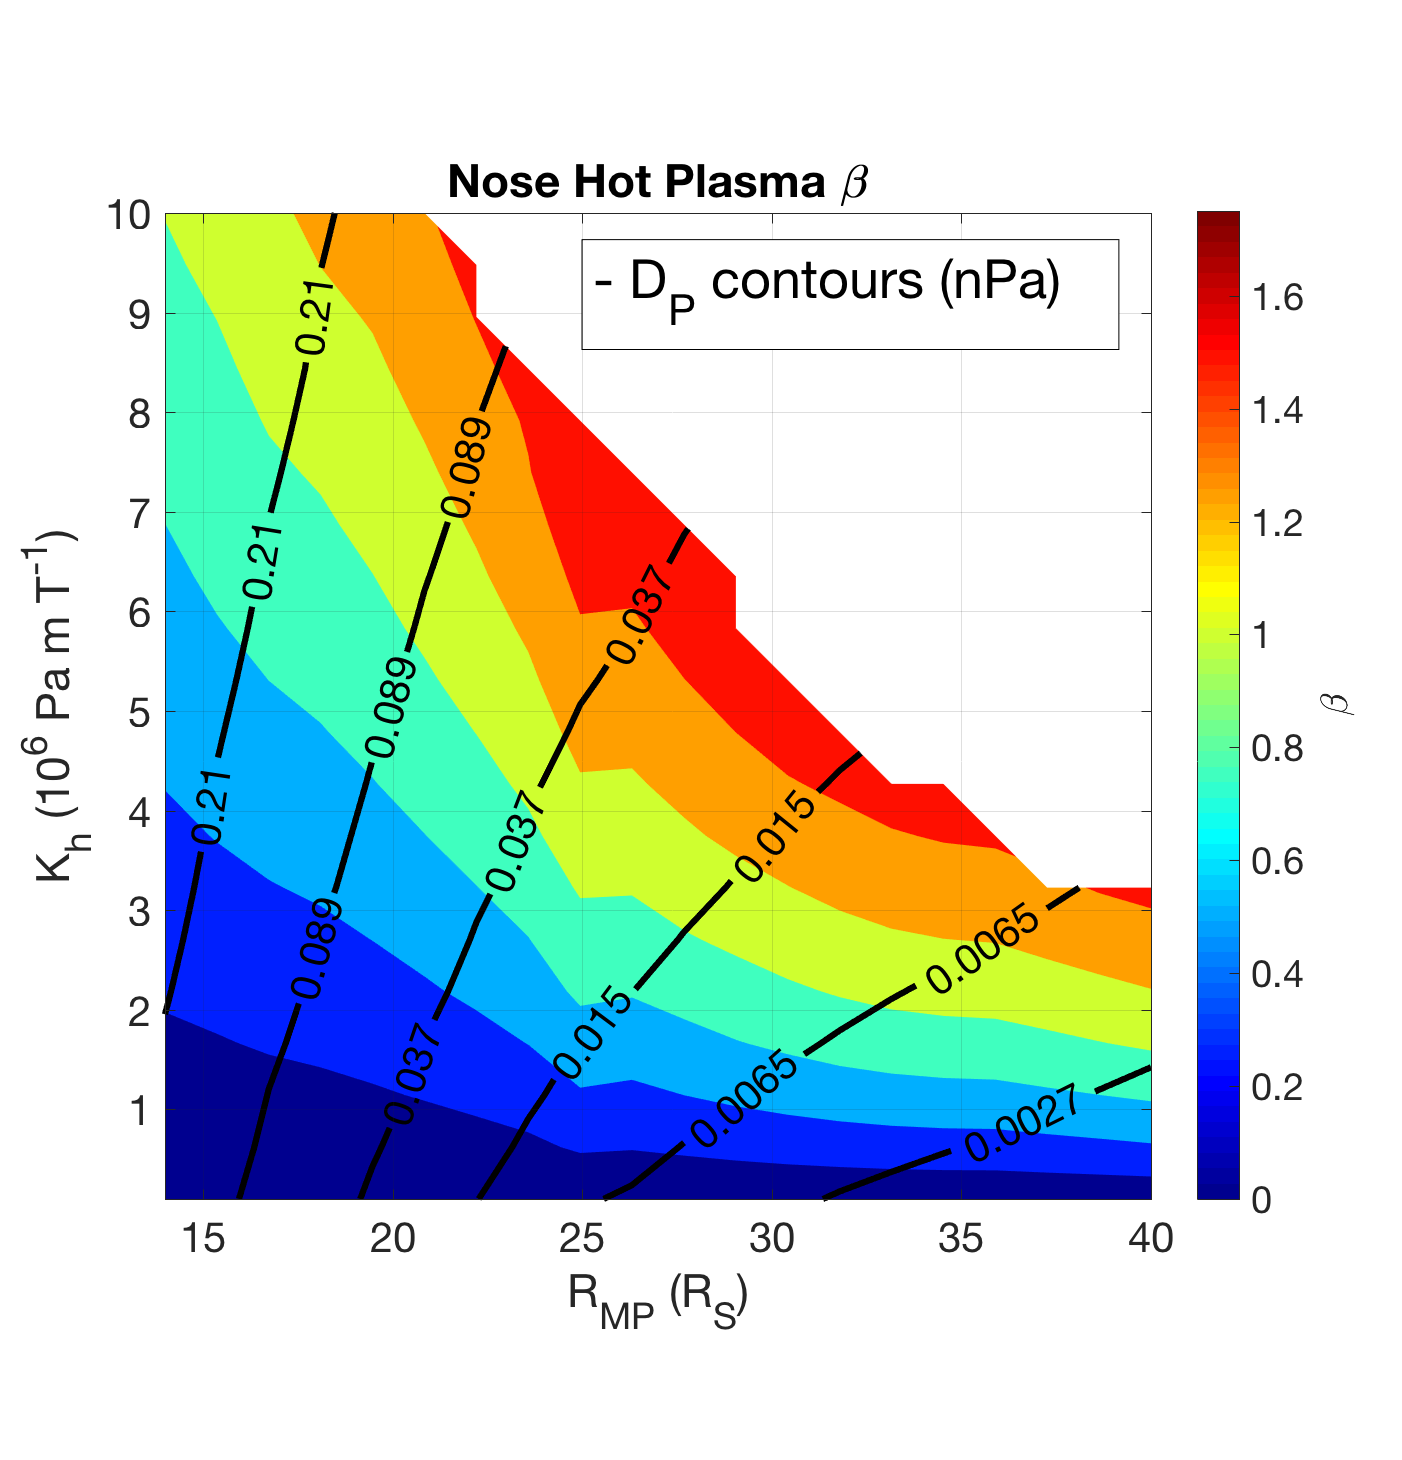
\includegraphics[width=0.7\textwidth]{compress/hotbetacontour.pdf}
\caption[Map of hot plasma $\beta$ just inside the magnetopause boundary in system size, $K_\mathrm{H}$ parameter space.]{Hot plasma $\beta$ at the nose of the magnetosphere just inside the magnetopause boundary, varying with both magnetopause radius $R_\mathrm{MP}$ and hot plasma index $K_\mathrm{H}$. The $\beta$ value is indicated on a colour scale. Contours of constant solar wind dynamic pressure $D_\mathrm{P}$ are shown as black lines, labelled with values in units of nPa.}
\label{compress:fig:hotbetacontour}
\end{figure}

For a dipolar magnetic field with isothermal plasma transport, it was explained in the introduction that we would expect $P_\mathrm{H} \propto r^{-4}$, thus giving $\alpha \approx 4$ for a magnetosphere with compressibility controlled by hot plasma content. However Figure \ref{compress:fig:alphas} shows we find $\alpha < 4$ in the most extreme cases. Indeed, when fitting the profiles of hot plasma pressure specifically for each $K_\mathrm{H}$ value, it was found that for these model calculations, the behaviour varied from $P_\mathrm{H} \propto r^{-3.3}$ for the smallest hot plasma index to $\propto r^{-2.6}$ for the greatest, corresponding to a reduction in compressibility parameter $\alpha$. It was also found that, unlike the magnetic pressure profiles, there was no considerable shift in behaviour at $\SI{25}{R_S}$, and so the observed kink in Figure \ref{compress:fig:hotbetacontour} in this region is solely due to change in magnetic pressure, the denominator of $\beta_\mathrm{H}$.

This behaviour of the hot plasma pressure can be further understood as follows. The parameterisation of hot plasma adopted in this model means that $P_\mathrm{H}$ is fully determined by how the flux tube volume varies with system size, as $P_\mathrm{H}V=K_\mathrm{H}$. The flux tube volume is defined in equation (\ref{compress:eq:ftv}), and is thus dependent on both the length of a given field line ($ds$) and the magnetic field strength ($B$). For a dipolar field line, $B \propto r^{-3}$ and $\int ds \propto r$, hence $V \propto r^4$ and $P_\mathrm{H} \propto r^{-4}$ in our parameterisation. However in this model, as we have discussed, we have found that the magnetic field strength varies more slowly with radial distance than this, particularly in expanded regimes and with high hot plasma content. Indeed the behaviour varies from $B \propto r^{-2.7}$ for compressed regimes with low hot plasma content, to $\propto r^{-1.8}$ for expanded regimes with high hot plasma content, corresponding to a more significant magnetodisc field. This in turn affects how flux tube volume varies with system size, meaning $P_\mathrm{H}$ varies more slowly with system size.

In addition, we also observed that for more expanded systems, the length of the outermost magnetic field lines $\int ds$ varied more slowly with radial distance than for a dipolar magnetic field, with $\int ds \propto r^{0.9}$ for magnetospheres with the lowest $K_\mathrm{H}$ values, to $\propto r^{0.8}$ for the highest $K_\mathrm{H}$ values. For more expanded, stretched magnetospheres, it is perhaps intuitive that the magnetic field lines in the outer regions have shorter overall lengths than a corresponding dipolar magnetic field line that crosses the equator at the same radial distance, due to the outward radial stretching of the dipole magnetic field associated with the ring current. Figure \ref{compress:fig:LCFL} illustrates this oblateness of the magnetospheric magnetic field lines observed in our model calculations, and how it increases with system size and hot plasma content. Each panel illustrates how the shape of the outermost closed magnetic field line, which crosses the equator at the magnetopause nose, varies with the size of the magnetosphere, for a given $K_\mathrm{H}$ value. The shape is shown in height above the rotational equator $Z$ and cylindrical radial distance from the planet centre $\rho$, normalized to the magnetopause radius $R_\mathrm{MP}$, with a representative dipolar magnetic field line shown in black on each plot for comparison.
\begin{figure}
\centering
\noindent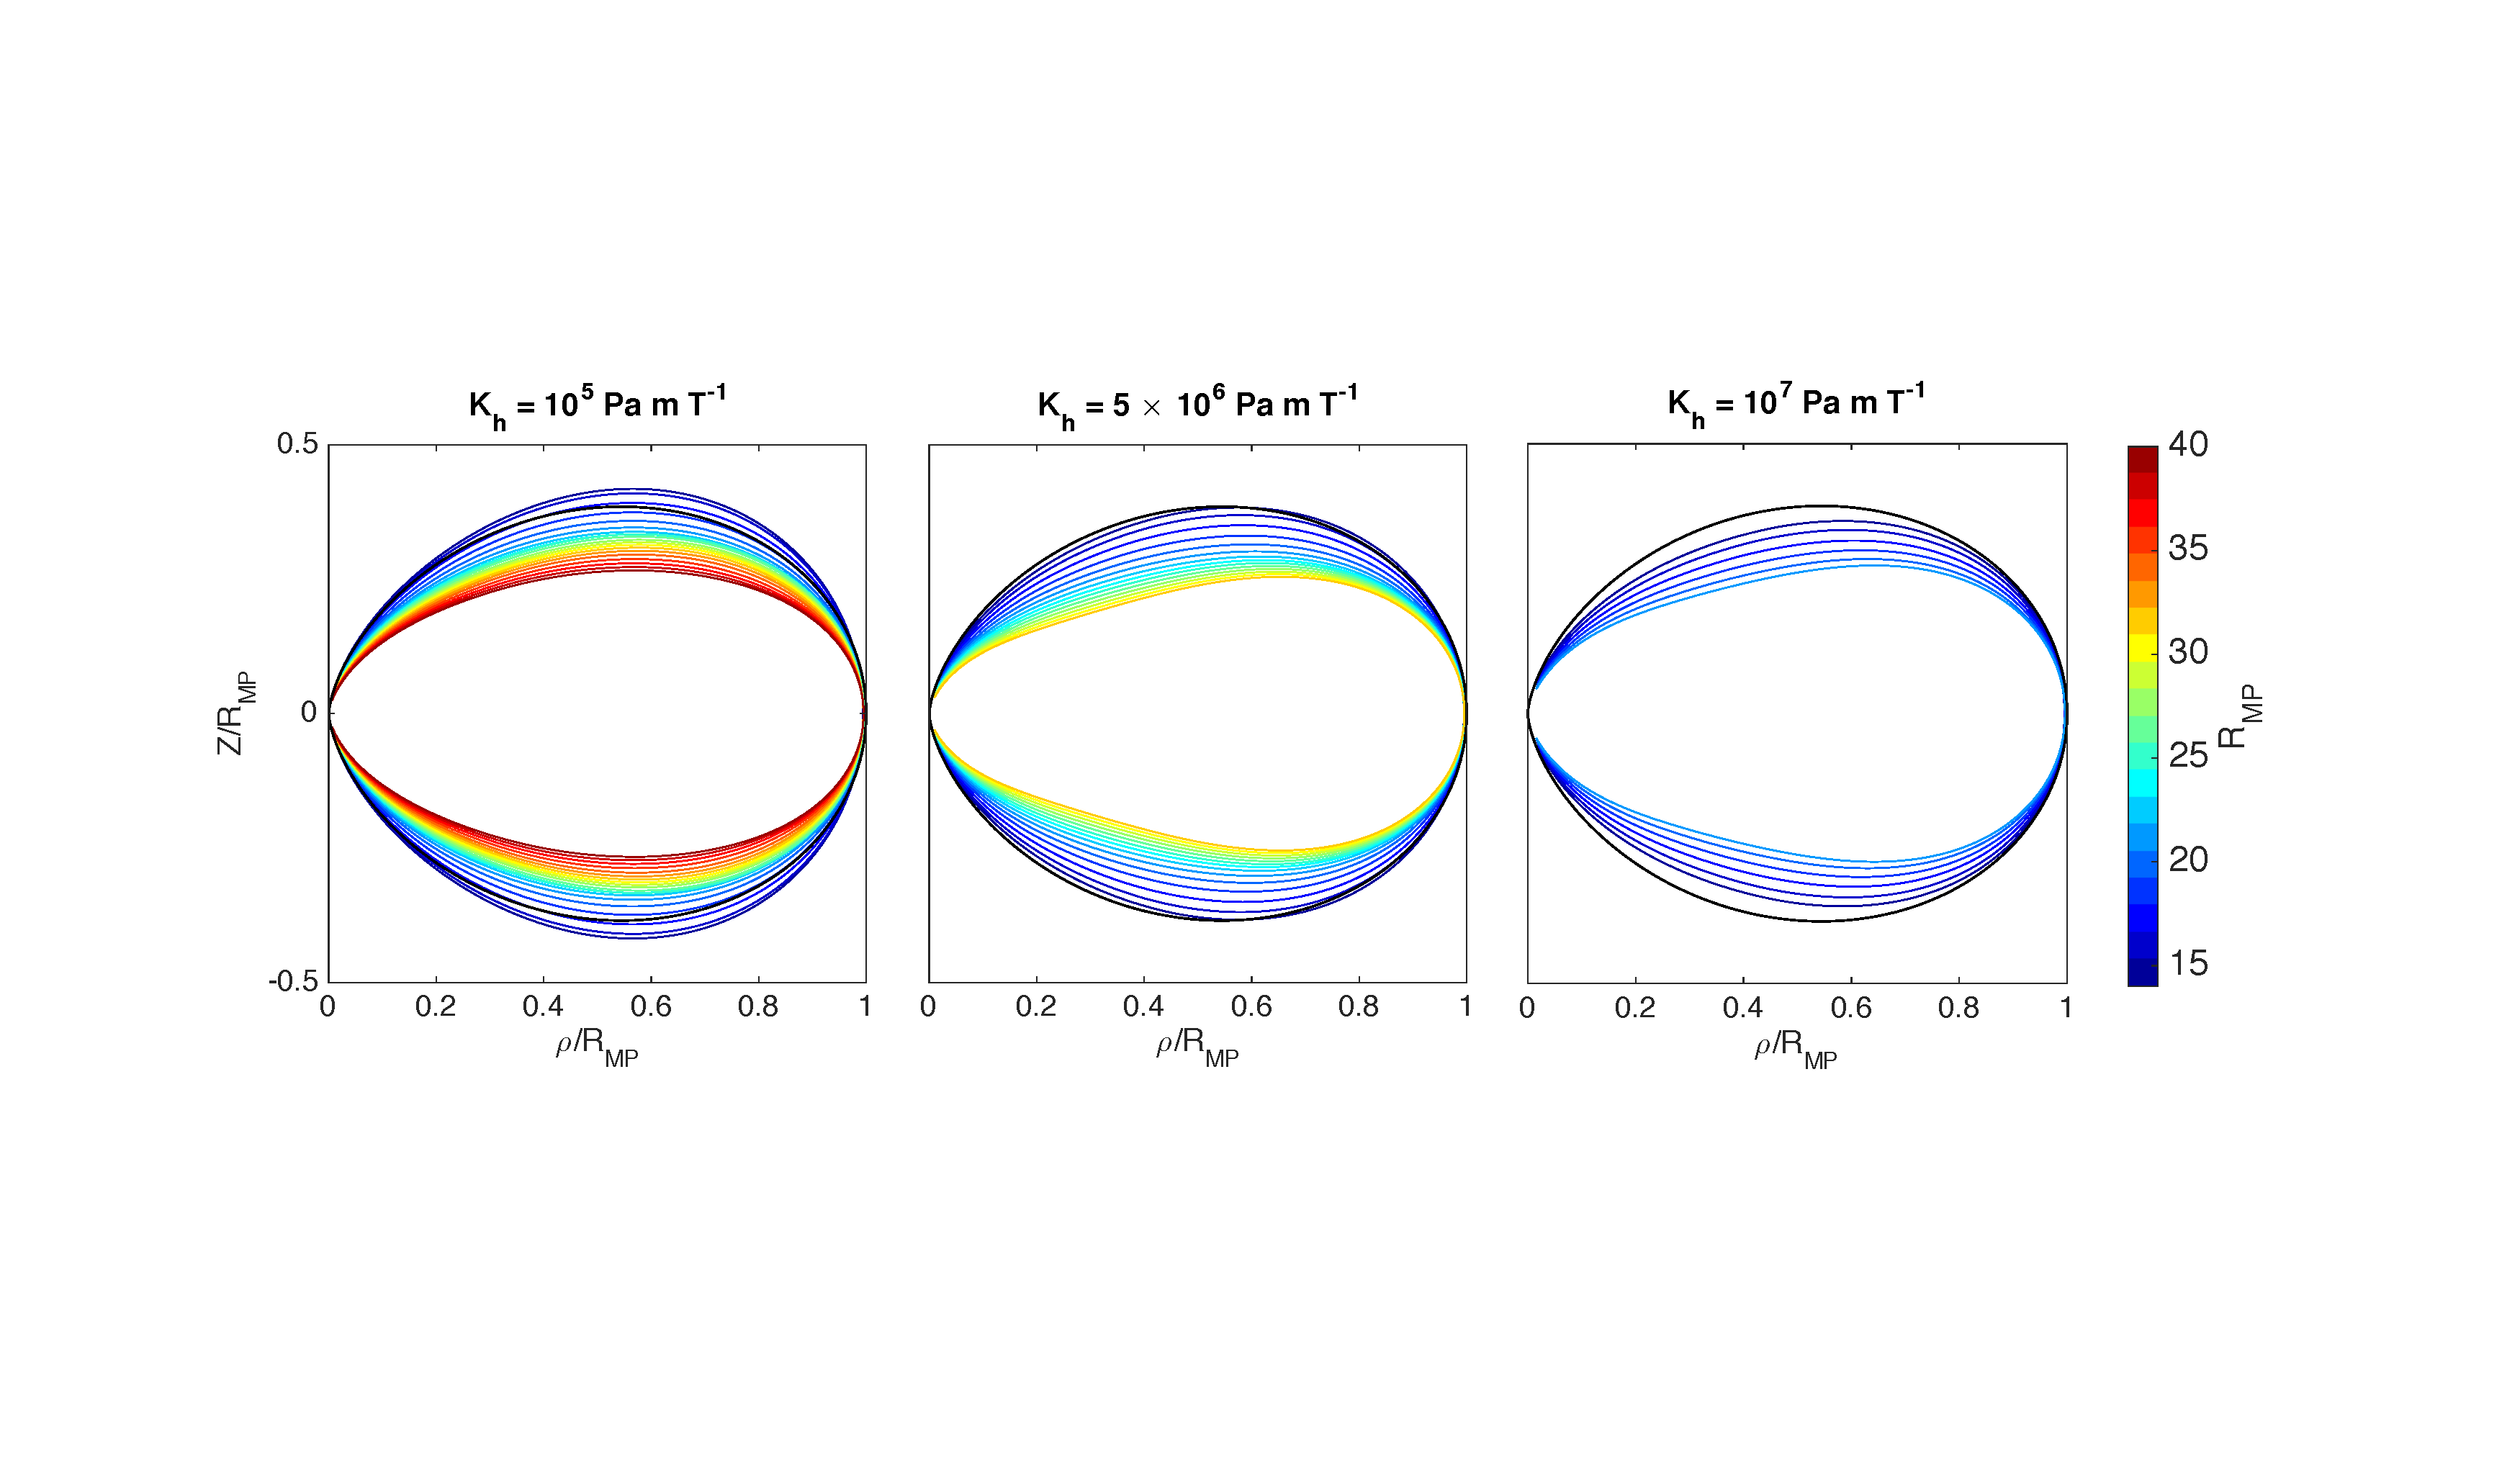
\includegraphics[width=\textwidth]{compress/LCFL.pdf}
\caption[Outermost magnetic field line shapes for the range in system size, $K_\mathrm{H}$ parameter space.]{The shape of the outermost closed field line in a magnetosphere as the magnetopause radius $R_\mathrm{MP}$ changes, for three different values of $K_\mathrm{H}$ corresponding to very quiet, average and disturbed ring currents respectively. In each panel the shape of the field line has been normalized in the vertical and horizontal direction by the magnetopause radius $R_\mathrm{MP}$, the value of which is shown by the colour of the field line according to the colour bar. A representative dipolar magnetic field line is shown in black on each plot for comparison.}
\label{compress:fig:LCFL}
\end{figure}

It can be seen clearly that as the magnetosphere size increases the outermost closed field line is confined comparatively much more towards the equator than for the magnetospheres with smaller $R_\mathrm{MP}$. This is especially pronounced for the magnetospheres with higher hot plasma content, where the field lines show significant oblateness particularly at lower $\rho$. 

This effect can be interpreted theoretically as follows. Considering pressure balance perpendicular to a magnetic field line in the outer magnetosphere, the two dominant forces to consider are the hot plasma pressure gradient and the centrifugal force. The force associated with the plasma pressure gradient acts outwards from the center of curvature of the field line, perpendicular to the field line, across the entire field line length. This property arises as a consequence of plasma pressure being assumed constant along a field line (see Section \ref{compress:sec:model}). In contrast, the centrifugal force acts in the direction of increasing $\rho$. Therefore the component of centrifugal force perpendicular to the magnetic field line can either act outwards away from or inwards towards the equatorial plane depending on the geometry, acting inwards for smaller $\rho$, and outwards beyond the `turning' point of the magnetic field line, when the field line begins to converge back towards the equator. This turning point occurs about half away along the magnetosphere, at around 0.5 $\rho/R_\mathrm{MP}$, for the compressed, low $K_\mathrm{H}$ cases, but as far out as 0.7 $\rho/R_\mathrm{MP}$ for the most expanded and hottest cases. The further out in radial distance that this turning point occurs, the higher the fraction of the magnetic field line for which the perpendicular component of centrifugal force is acting inwards, towards the equatorial plane - and thus effectively balancing the outwards hot plasma pressure gradient force. Therefore in order to maintain global force balance, this turning point moves radially outwards as the hot plasma pressure gradient increases, and the field line thus becomes more confined.

We explained in Section~\ref{compress:sec:model} that the parameterisation of hot plasma content via the state equation involving the index $K_\mathrm{H}=P_\mathrm{H}V$ was a simplifying assumption in light of variable observations of hot plasma pressure. However it would have also been possible to instead parameterise the hot plasma content by, for example, $K_\mathrm{H}=P_\mathrm{H}V^\gamma$, with $\gamma=5/3$, such that magnetic flux tubes of plasma are considered to expand and contract adiabatically rather than isothermally. The factors of $B$ and $\int ds$ that determine the flux tube volume $V$ would be unchanged, however the previous relationship $P_\mathrm{H}\propto V^{-1}$ would be modified to $P_\mathrm{H} \propto V^{-\gamma}$. For a magnetosphere with compressibility controlled by hot plasma content, this corresponds to an increase in the estimate of the compressibility parameter $\alpha$ by a factor of $\gamma$, and thus a magnetosphere that is less sensitive to changes in solar wind dynamic pressure. This aspect may also contribute to the discrepancy between our results and those of previous empirical studies, shown in Figure~\ref{compress:fig:alphas}, as the plasma population may behave intermediately between the two state equations discussed in this study. Indeed, the analysis of \citet{achilleos2010a} supports this conclusion.

\subsection{Comparison with the Jovian System}\label{compress:sec:jup}
It is insightful to make a comparison between the results presented here and the corresponding calculations for Jupiter's magnetosphere, using our implementation of the model of \citet{caudal1986} directly. Figure~\ref{compress:fig:jupmoney} shows the results for Jovian calculations analogous to Figure~\ref{compress:fig:money1} for the Saturn case. Jovian magnetopause radii in the range $R_\mathrm{MP} = 50{\--}\SI{100}{R_J}$ have been used to cover the observed range presented in previous studies \citep{joy2002}.
\begin{figure}
\centering
\noindent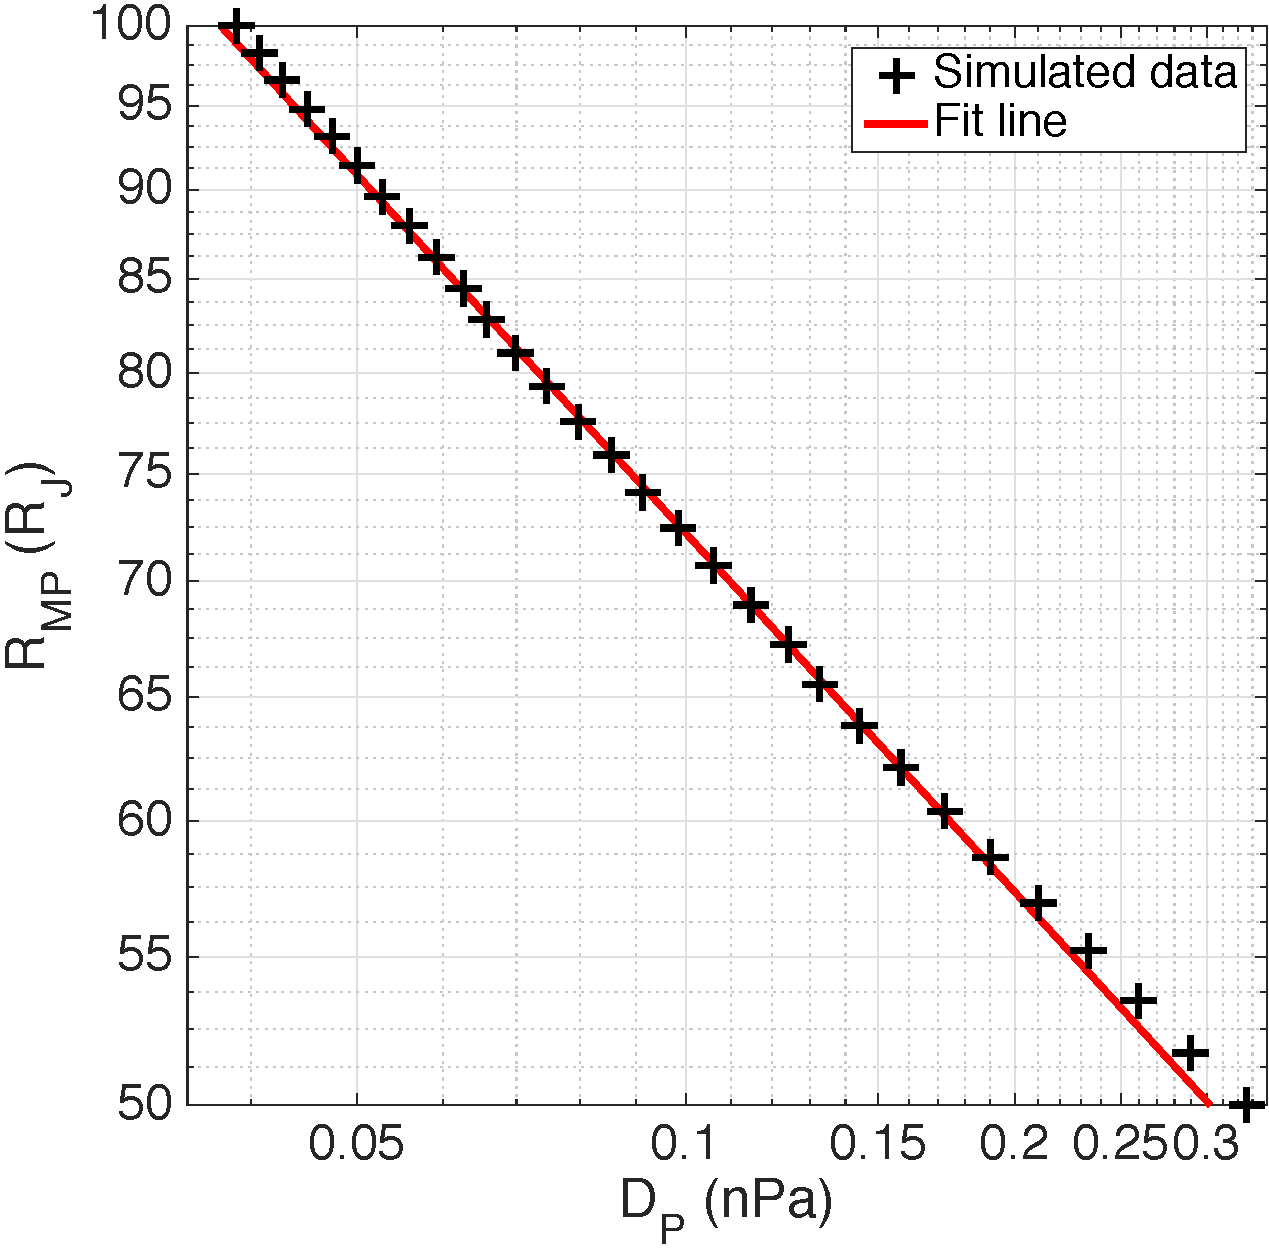
\includegraphics[width=0.7\textwidth]{compress/jupmoney.pdf}
\caption[Magnetopause radius versus solar wind dynamic pressure profile for Jupiter's magnetosphere.]{Magnetopause radius $R_\mathrm{MP}$ as a function of solar wind dynamic pressure $D_{P}$, on a logarithmic scale, for the magnetosphere of \textbf{Jupiter}. Each black cross represents the result of one model calculation. The linear least squares regression line fitted to calculations is shown in red.}
\label{compress:fig:jupmoney}
\end{figure}

It can clearly be seen that, unlike the Saturn case, the Jovian magnetosphere shows a compressibility behaviour that is well represented by a uniform $\alpha$ across all observed system sizes, demonstrated by a constant gradient of the $D_\mathrm{P}$ profile. A single linear least squares regression line fit provided an estimate for the compressibility parameter $\alpha=3.05 \pm 0.02$. As for the Saturn case, the data were split into two groups representing a compressed and expanded regime, and a linear least squares regression line was fit to each group separately. However, this did not provide significantly different estimates for $\alpha$, with a variation of only approximately 6$\%$ between groups, and so only the fitting for the entire simulated data set is shown and discussed here. This value of $\alpha=3.05 \pm 0.02$ is remarkably smaller than observational studies in the literature, which estimate this value as between ${\sim}4$ and ${\sim}5$ \citep{huddleston1998,joy2002,alexeev2005}. Possible reasons for this discrepancy are discussed at the end of this section. However it can be seen from a comparison with Figure \ref{compress:fig:alphas} that this value is consistent with our original theoretical expectation that this value be lower than that of the Saturn system, due to arguments discussed in Section~\ref{compress:sec:intro}.

It is worth noting that this difference in behaviour between the Saturnian and Jovian magnetospheres is also a consequence of their relative locations in the solar system, and the weaker solar wind dynamic pressure experienced at Saturn. If Saturn were to be located closer to the Sun such that it experienced the higher solar wind dynamic pressures typically observed at Jupiter, then the Saturnian magnetosphere would also show a compressibility behaviour represented by a uniform $\alpha$, specifically corresponding to its compressed regime. This can be seen by comparing the ranges in solar wind dynamic pressure in Figure \ref{compress:fig:money1} and Figure \ref{compress:fig:jupmoney}.

We compared the individual $P_\mathrm{H}$, $P_\mathrm{C}$ and $P_\mathrm{B}$ components that comprise the $D_\mathrm{P}$ estimate across all system sizes and found that, as with the initial results for the Saturn case presented in Figure~\ref{compress:fig:pcomps}, the magnetic pressure component was dominant across all system sizes. Both hot and cold plasma $\beta$ monotonically increased with system size, with $\beta_\mathrm{C} \leq 0.3$ and $\beta_\mathrm{H} \leq 0.8$ across the simulated data set. Unlike the Saturn case, there was no evidence of a shift in gradient of the magnetic pressure ($P_\mathrm{B}$) profile for increased values of $R_\mathrm{MP}$; we measured a constant slope equivalent to $P_\mathrm{B}\propto r^{-3.4}$, corresponding to $B\propto r^{-1.7}$. This index is smaller than was measured even in the hottest and largest magnetosphere models in our Saturn investigation, and corresponds to a very significant disc-like distortion from a dipolar magnetic field for all Jupiter $R_\mathrm{MP}$. Comparable behaviour is expected theoretically as discussed in Section~\ref{intro:sec:comparativemagnetospheres} of this thesis, and has also been observed empirically \cite[e.g.][]{khurana1989}. We also found that the hot plasma pressure $P_\mathrm{H}$ varied as $P_\mathrm{H} \propto r^{-2.7}$, comparable to the behaviour measured for the hottest and largest magnetosphere models in our Saturn investigation. This can readily be explained via the same arguments applied to the Saturn case in the previous section.

As with our initial Saturn investigation, we estimated the pressure contribution from the centrifugal force at the magnetopause boundary, using a very approximate value for the magnetopause boundary layer thickness of $\SI{1}{R_J}$ following \citet{delamere2010}. We found that the centrifugal term was at least an order of magnitude smaller than all other pressure components at the magnetopause boundary across all system sizes, and therefore does not play a significant role in determining compressibility. However in a study by \citet{nichols2011}, it was suggested that this Jovian model may significantly underestimate the magnitude of centrifugal force in the middle and outer magnetosphere, due to the use of a plasma angular velocity profile that overestimates the breakdown of corotation. This would mean that the model would also overestimate how strongly the centrifugal force falls with radial distance. In combination, these effects may contribute to the discrepancy between our particularly low estimate of the compressibility parameter $\alpha$ for the Jovian magnetosphere, and previous empirical studies. While beyond the scope of the  current work,  it  would be insightful to investigate this aspect further in future studies, as well as the influence of different hot plasma parameterisations, using more recent spacecraft data sets than the Voyager results employed in the \citet{caudal1986} model.

\section{Summary and Conclusions}
We have employed a 2D force-balance model of Saturn's dayside magnetosphere, first described in \citet{achilleos2010a}, to investigate magnetospheric compressibility, and in particular its response to solar wind conditions and global hot plasma content. We have found that, for `average' global hot plasma conditions, the compressibility behaviour can be described by equation~\ref{compress:eq:key} but with a value of compressibility parameter $\alpha$ that decreases with system size, from ${\sim}4.8$ for $R_\mathrm{MP} \leq \SI{25}{R_S}$ to ${\sim}3.5$ for $R_\mathrm{MP} > \SI{25}{R_S}$. This corresponds to the magnetosphere becoming more easily compressible as the upstream solar wind dynamic pressure decreases. We have explained this in terms of the distortion of the magnetic field into a magnetodisc configuration, which is more easily compressible than a dipolar magnetic field, and that this distortion becomes significant for more expanded magnetospheres. 

We have shown that the global hot plasma content of the magnetosphere, parameterised by the hot plasma index $K_\mathrm{H}=P_\mathrm{H}V$, also plays an important role in determining magnetospheric compressibility. When Saturn's magnetosphere is compressed, a higher value of $K_\mathrm{H}$ acts to increase the observed magnetospheric compressibility via an enhancement of the aforementioned magnetodisc magnetic field structure, due to its contribution to the associated ring current magnetic field. When the magnetosphere is more expanded, the hot plasma pressure exceeds the magnetic pressure at the magnetopause boundary such that the variation in hot plasma pressure with radial distance becomes significant in controlling magnetospheric compressibility. We have determined that, as the hot plasma pressure $P_\mathrm{H}$ varies more slowly with radial distance than the magnetic pressure $P_\mathrm{B}$, this corresponds to the magnetosphere becoming more easily compressible under such conditions. We also explored the behaviour of the $P_\mathrm{B}$ and $P_\mathrm{H}$ profiles, and how they are related via the flux tube volume $V$. Our estimates of $\alpha$ are in the range ${~}3.3-5.3$ depending on system size and hot plasma content, with lower estimates corresponding to higher values of both of these parameters. However as we have mentioned, these results are sensitive to our simplifying parameterisation of the hot plasma content, and for example would increase up to a factor of $5/3$ (for regions of parameter space where hot pressure is dominant) if we were instead to parameterise the hot plasma content via $K_\mathrm{H} = P_\mathrm{H}V^\gamma$. 

These results thus suggest that future observational studies of the relationship between $R_\mathrm{MP}$ and $D_\mathrm{P}$ may benefit from the assumption that the compressibility parameter $\alpha$ is not constant across all observations, but varies both with system size and hot plasma content, at comparable levels of significance. In addition, our model analysis demonstrates that centrifugal force at the magnetopause boundary does not contribute significantly to the compressibility of the magnetosphere. On the other hand, \textit{global} centrifugal force is important in determining the global field structure, and thus, compressibility. Improvements are needed in our treatment of the plasma angular velocity profile, in order to make it self-consistent with the changing magnetic field structure so as to further test our initial findings.

The investigation in  this chapter has demonstrated in detail how the magnetic field and plasma structure in the \citet{achilleos2010a} model varies with internal hot plasma conditions, and with system size. In particular, the result that the magnetospheric magnetic field becomes more disc-like as it expands, is utilised in the study presented in the next chapter. In Chapter~\ref{chap:equinox}, we investigate the periodic `flapping' and `breathing' behaviour of Saturn's equatorial current sheet, introduced in Section~\ref{intro:sec:periodicities}.  This breathing behaviour  corresponds to a periodic thickening and thinning of the current sheet at different Saturn  longitudes, associated with a reconfiguration from a more dipolar to a more disc-like magnetic field; we use a modified version of the \citet{achilleos2010a} model calculated at different system sizes to represent this periodic variation.
\chapter[The Periodic Flapping and Breathing of Saturn's Magnetodisc]{The Periodic `Flapping' and `Breathing' of Saturn's Magnetodisc During Equinox}
\label{chap:equinox}
In this chapter, we present the results of an investigation into the periodic displacement and thickness modulation of the equatorial current sheet at Saturn. Periodic variations have been observed in many field and particle properties in Saturn's magnetosphere, modulated at a period close to the planetary rotation rate. Pertinent to this study, magnetic field observations by \textit{Cassini}'s MAG instrument suggest that in the outer magnetosphere (beyond ${\sim}\SI{12}{R_S}$) Saturn's current sheet is periodically displaced with respect to the rotational equator, to a first approximation acting as a rotating, tilted disc. This manifests as a `flapping' mode when observed by the spacecraft. Recent studies suggest the magnetosphere also has a `breathing' mode, expanding and contracting with a period close to the planetary rotation rate, correlating with a modulation in the thickness of the equatorial current sheet. In this chapter, we model these two modes in tandem by combining a global, geometrical model of a tilted and rippled current sheet with the UCL/AGA force-balance model of Saturn's magnetodisc presented in Section~\ref{intro:sec:forcebalancemodel}, accounting for the magnetospheric size and hot plasma content. We simulate the breathing behaviour by introducing an azimuthal dependence of the system size. We fit Cassini MAG data acquired on equatorial orbits from 23 Oct{\--}17 Dec 2009 (Revs 120{\--}122), close to Saturn equinox, in order that seasonal effects on the current sheet are minimised. We find that our model characterises well the amplitude and phase of the oscillations in the data, for those passes that show clear periodic signatures in the field. In particular, the $B_\theta$ (meridional) component can only be characterised when the breathing mode is included. This study introduces calculations for an oscillating boundary, which provide a basis for understanding the complex relationship between current sheet dynamics and the periodic field perturbations. 

The contents of this chapter are based on the study:

\bibentry{sorba2018}.

\section{Introduction}\label{equinox:sec:intro}
Recent observations of Saturn's magnetic field suggest that the planetary dipole axis and rotation axis are aligned to $\leq\SI{0.01}{\degree}$ \citep{dougherty2018}. However despite this extremely high degree of axisymmetry, periodic variations have been observed in field and particle properties throughout Saturn's magnetosphere, modulated at a period close to the planetary rotation rate. These observations are summarised in \citet{carbary2013}, and also discussed in Section~\ref{intro:sec:periodicities} of this thesis. Of particular interest to the study in this chapter are  the periodic perturbations observed in the magnetic field, and the influence  they have on global magnetospheric structure.

Even before the \textit{Cassini} mission arrived at Saturn, analysis of legacy magnetometer data from the \textit{Voyager} and \textit{Pioneer} missions had revealed periodic perturbations in the magnetic field, which could not be adequately explained by a true dipole tilt \citet{espinosa2000}. This led to the development of a `camshaft' model, where a rotating equatorial magnetic anomaly that is fixed in planetary longitude triggers radial waves that propagate through the magnetosphere and cause the observed perturbations \citep{espinosa2003b}. To further complicate the picture, \textit{Cassini} magnetic field observations then revealed two distinct periods in the magnetic field perturbations, associated separately with the Northern and Southern hemispheres \citep[e.g.][]{andrews2010,provan2012}. In these and other studies, such as \citet{hunt2014}, a picture has now been developed of how these hemispheric magnetic perturbations are generated, by two large-scale field-aligned current systems that rotate at slightly different rates in each hemisphere. The magnetic field associated with each current system is dominant in the respective hemisphere, and can be approximated in the outer magnetosphere by a rotating, transverse oriented dipole. The physical origins of these current systems are also still not fully understood, but are thought to be associated with twin atmospheric vortices flowing in the polar upper atmosphere/ionosphere in each hemisphere \citep{jiaandkivelson2012, southwood2014, smith2016}. During the initial \textit{Cassini} mission, the southern magnetic perturbation was dominant over the northern, and had a longer period of ${\sim}\SI{10.8}{\hour}$ compared to ${\sim}\SI{10.6}{\hour}$. However after Saturn equinox in August 2009, the two perturbations slowly converged in terms of both time period and amplitude, before diverging again \citep{andrews2012}.

In this study we focus on the effect of these dual rotating magnetic perturbations on Saturn's outer magnetosphere. To do this, it is helpful to first consider the picture put forth in \citet{andrews2010, provan2011} and references therein, of the two hemispheric perturbations being approximated by rotating transverse dipoles, each with associated magnetic field only felt in the respective hemisphere. In the magnetosphere's equatorial `core' region, within radial distances of ${\sim}10{\--}\SI{15}{R_S}$ and thus within the magnetic shells of the associated field-aligned currents \citep[e.g.][]{southwood2007}, the resulting magnetic perturbation field is rotating and quasi-uniform in magnitude. On higher-latitude field lines, and beyond the core region, the perturbation field can be approximated in each hemisphere by a dipole magnetic field whose axis lies in the rotational equatorial plane. The influence of these magnetic perturbations on the global magnetodisc structure is shown by the diagram in Figure~\ref{equinox:fig:CowleyTDdiagrams}, reproduced from \citet{cowley2017a}. The magnetospheric magnetic field, made up of Saturn's planetary dipole field and the magnetodisc field, is shown by the black lines in panels (a) and (c), whilst the perturbation fields associated with the Northern and Southern hemispheres are shown in blue and red respectively. The effect of these perturbation fields on the total magnetospheric magnetic field is then shown by the black lines in panels (b) and (d). The direction in which the effective `transverse dipole' points can be ascertained via an analysis of the oscillations in the magnetic field data \citep[e.g.][]{provan2009}, defined in each hemisphere by a phase $\Psi_\mathrm{N,S} = \SI{0}{\degree}$ and thus used to define a physically meaningful longitude system for the planet.
\begin{figure}
\centering
\includegraphics[width=0.9\textwidth]{equinox/cowleyTDdiagrams.pdf}
\caption[Sketches of hemispheric rotating magnetic perturbation fields, from \citet{cowley2017a}.]{Sketches showing the planetary magnetodisc magnetic field in black lines, and the magnetic field associated with the northern and southern hemispheric magnetic perturbations, in blue and red respectively. Panels (b) and (d) show the result of the superposition of the magnetodisc and perturbation magnetic fields shown in (a) and (c). Reproduced from \citet{cowley2017a}.}
\label{equinox:fig:CowleyTDdiagrams}
\end{figure}

A key effect of these magnetic perturbations on Saturn's magnetodisc is a periodic motion of the equatorial current sheet above and below the rotational equator, or `flapping' behaviour as perceived by a stationary observer. This is a separate phenomenon to the displacement of the entire current sheet northwards into a bowl-like shape observed by \citet{arridge2008warp} during the initial \textit{Cassini} mission, which was due to the incoming direction of the solar wind plasma impacting the magnetopause from the south during Saturn's southern summer. In the transverse dipole approximation, this flapping we describe can be understood as follows. At $\Psi_\mathrm{N,S} = \SI{0}{\degree}$, the radial component of the perturbation field adds to the planetary magnetodisc field north of the equator, and subtracts from the background field south of the equator. The opposite is true at $\Psi_\mathrm{N,S} = \SI{180}{\degree}$. Magnetic pressure balance must be approximately maintained across the lobes of (regions just outside) the current sheet and thus this has the net effect of a rotating perturbation, acting to displace the equatorial current sheet southward below the rotational equator at the particular longitude defined by $\Psi_\mathrm{N,S} = \SI{0}{\degree}$, and northward at the diametrically opposite longitude, as shown in Figure~\ref{equinox:fig:CowleyTDdiagrams} b, d. As the whole pattern rotates, this rotating tilted magnetodisc appears to a stationary observer as a periodic vertical flapping of the current sheet, as it passes above and then below the rotational equator once per rotation period. 

This behaviour has been detected, and quantified to some extent, in studies using various \textit{Cassini} datasets. In \citet{southwood2007}, the authors analysed signatures of periodic equatorial current sheet crossings observed in the magnetic field data measured by \textit{Cassini's} magnetometer (MAG) instrument on equatorial orbits in 2006. They determined that, in the outer magnetosphere beyond ${\sim}12{\--}\SI{15}{R_S}$, the total magnetic field can be approximated by a rotating tilted disc, with a tilt angle of ${\sim}12{\--}\SI{15}{\degree}$ relative to the spin axis. This is in broad agreement with a study by \citet{arridge2011}, who fitted a model of a tilted and rippled current sheet to MAG and CAPS/ELS data from orbits from 2006. They found that a value of $\SI{12}{\degree}$ for the effective current sheet tilt provided a good agreement between their model and the data, and that smaller values could not reproduce the amplitudes of the oscillations in the data. In contrast, in \citet{provan2009} the authors analysed magnetic field data from subsequent higher-latitude \textit{Cassini} orbits and found smaller values for an effective dipole tilt of ${\sim}5{\--}\SI{10}{\degree}$, and that the best fit value depended on the component of the magnetic field vector being analysed. 

As pointed out in \citet{provan2009}, this kind of analysis does not establish the influence of the relative phases of the southern and northern perturbations on the current sheet flapping. The studies discussed so far are based on \textit{Cassini} observations made when the southern perturbation was dominant in amplitude, and thus the observed current sheet tilt was associated with this perturbation only. However, as previously mentioned, after Saturn equinox the two perturbations became similar in amplitude, and so it is important to consider the effect of both. Figure~\ref{equinox:fig:CowleyTDdiagrams} illustrates that a maximum current sheet displacement would be observed when the two perturbations are in phase, such that the meridians defined by $\Psi_\mathrm{N} = \SI{0}{\degree}$ and $\Psi_\mathrm{S} = \SI{0}{\degree}$ spatially coincide, and a minimum displacement arises when these meridians are diametrically opposite, and the perturbations are in antiphase. Indeed \citet{provan2012} observed in the magnetic field data that the current sheet oscillation was a maximum when the two perturbations were in phase, and some modelling studies such as \citet{jiaandkivelson2012} and \citet{cowley2017a} have also investigated this kind of behaviour. However there is still much to be understood, particularly for intermediate perturbation phase differences, and the effect of the change of phase with radial distance in the outer magnetosphere. In this study we look at these effects in more detail.

The other important effect of these magnetic perturbations is the current sheet `breathing' behaviour. That is, a compressional disturbance in the magnetodisc. While the rotational disturbance that causes the flapping behaviour is mainly associated with the \textit{radial} component of the perturbation magnetic field, the compressional disturbance is mainly associated with the \textit{meridional} component. Again looking at Figure~\ref{equinox:fig:CowleyTDdiagrams}, we can see that for the northern perturbation, the meridional component subtracts from the planetary magnetodisc field at $\Psi_\mathrm{N} = \SI{0}{\degree}$, and adds at $\Psi_\mathrm{N} = \SI{180}{\degree}$. In contrast for the southern perturbation, the meridional component adds to the planetary magnetodisc field at $\Psi_\mathrm{S} = \SI{0}{\degree}$, and subtracts at $\Psi_\mathrm{S} = \SI{180}{\degree}$. Where the perturbation field enhances the planetary magnetic field, this causes a compression of the magnetic field lines into a more dipolar configuration, associated with a thickening of the equatorial current sheet, observed by a stationary observer as a `breathing in'. At the opposite longitude, the reduction in the meridional component of the magnetodisc magnetic field causes an extension of the magnetic field lines into a more disc-like configuration, associated with a thinner and more extended current sheet. Unlike the case of the flapping perturbation, this breathing perturbation occurs at opposite phase longitudes for each hemisphere, and so we would expect to observe a maximum compressional disturbance when the northern and southern perturbations are $\SI{180}{\degree}$ out of phase.

This behaviour was also observed in \citet{provan2012}, who found that the thickness of the current sheet was modulated by a factor of ${\sim}2$ when the magnetic perturbations were in antiphase. More recently, \citet{thomsen2017} looked in detail at the expected magnetic field signatures for intermediate perturbation field phase relationships, as a companion study to \citet{cowley2017a}. These studies found instances of `sawtooth' shaped signatures in the magnetic field data during current sheet crossings, and, through a comparison with various modelling results, suggested that this was associated with a periodic thickening and thinning of the magnetospheric current sheet. A further study by \citet{cowley2017b} suggests a complex relationship between current sheet thickness in each hemisphere and intermediate perturbation phase differences. In MHD modelling studies there is also evidence for this periodic breathing behaviour in the middle magnetosphere \citep{ramer2016}, and a periodic perturbation in the magnetopause boundary location \citep{kivelson2014}, which may be related. As previously mentioned, \citet{clarke2010} also found evidence using \textit{Cassini} magnetometer data that the magnetopause boundary moves periodically by up to $\SI{5}{R_S}$ in the post-noon local time sector.

In this study we attempt to draw these various strands together, and investigate both the flapping and breathing behaviour of Saturn's magnetodisc. We use a local, force-balance magnetic field and plasma model of Saturn's magnetodisc adapted from \citet{achilleos2010a} (the UCL/AGA model), and anchor it to a global, geometric model of the current sheet location adapted from \citet{arridge2011} in order to model a magnetodisc that displays both behaviours. We compare our model magnetic field predictions to measurements made by \textit{Cassini's} magnetometer on three equatorial orbits made shortly after Saturn equinox in August 2009, in order that the aforementioned seasonal effect on the current sheet shown by \citet{arridge2008warp} is minimised. We fit parameters that describe the tilt of the current sheet, and the longitudes of the maximum rotational (flapping) and compressional (breathing) disturbances, for each \textit{Cassini} pass in order to quantitatively understand how the relative phase of the hemispheric magnetic perturbations affects the magnetodisc structure. In Section \ref{equinox:sec:method} we discuss how the tilted, rippled current sheet model from \cite{arridge2011} simulates the flapping of the current sheet. We also describe our use of the UCL/AGA model, how we choose appropriate model parameters for our data set, and the modifications we make to it in this study. We also explain how we simulate breathing behaviour by varying the UCL/AGA magnetodisc model radius we use as a function of longitude. In Section~\ref{equinox:sec:results} we discuss the best fit parameters we find for each \textit{Cassini} pass in our data set, and what they indicate regarding the variability of the flapping and breathing behaviour. We conclude with a summary and discussion of potential future work in Section~\ref{equinox:sec:conclusions}.

\section{Method}\label{equinox:sec:method}
\subsection{Data}
In this study we analysed \textit{Cassini} magnetometer data acquired on three equatorial orbits from 23 October{\--}17 December 2009 (Revs 120{\--}122), closely following Saturn equinox in August 2009. This interval was chosen in order that the seasonal effect of the current sheet deformation into a `bowl' shape \citep[e.g.][]{arridge2008warp} is minimised, and the current sheet is crossed numerous times. We only analysed data observed beyond \SI{12}{R_S} in cylindrical radial distance relative to the rotation / dipole axis, where we expect this dynamical behaviour of the current sheet to occur. The choice of \SI{12}{R_S} in particular is discussed in detail in the next section. The data set was further restricted to ensure all observations are made within the magnetosphere proper by comparing with the list of magnetopause crossings made by \textit{Cassini} provided in the study by \citet{pilkington2015}, and comparing local MAG and CAPS-ELS observations to signatures described in that study, to determine whether \textit{Cassini} was inside or outside the magnetosphere at a given time. We further excluded data within 6 hours of a magnetopause crossing.

These trajectories are shown by the red-blue path in Figure~\ref{equinox:fig:cassinitrajectory}, with Saturn shown by the solid circle at the origin. The KSMAG coordinate system used represents a rotation about the $y$ axis of the more standard KSM coordinate system. In KSMAG, the $z$ axis points along Saturn's rotation/dipole axis, the $x$ axis is oriented such that the $x-z$ plane contains the planet-Sun direction, and the $y$ axis completes the right-handed set. A typical model magnetopause surface from \citep{pilkington2015} is shown by the black dashed line. In this data set the maximum radial distance of \textit{Cassini} from the planet is ${\sim}\SI{42.4}{R_S}$, the maximum distance of \textit{Cassini} above/below the rotational equator is $z_\mathrm{KSMAG}\approx +0.3/\SI{-1.2}{R_S}$, and the range in magnetic local time is ${\sim}$15:45 to 22:45. Since the spacecraft flies close to the rotational equator throughout this interval, we would expect to see near-symmetric oscillations in the radial component of the magnetic field, if the mean position of the current sheet also lies close to the rotational equator.
\begin{figure}
\centering
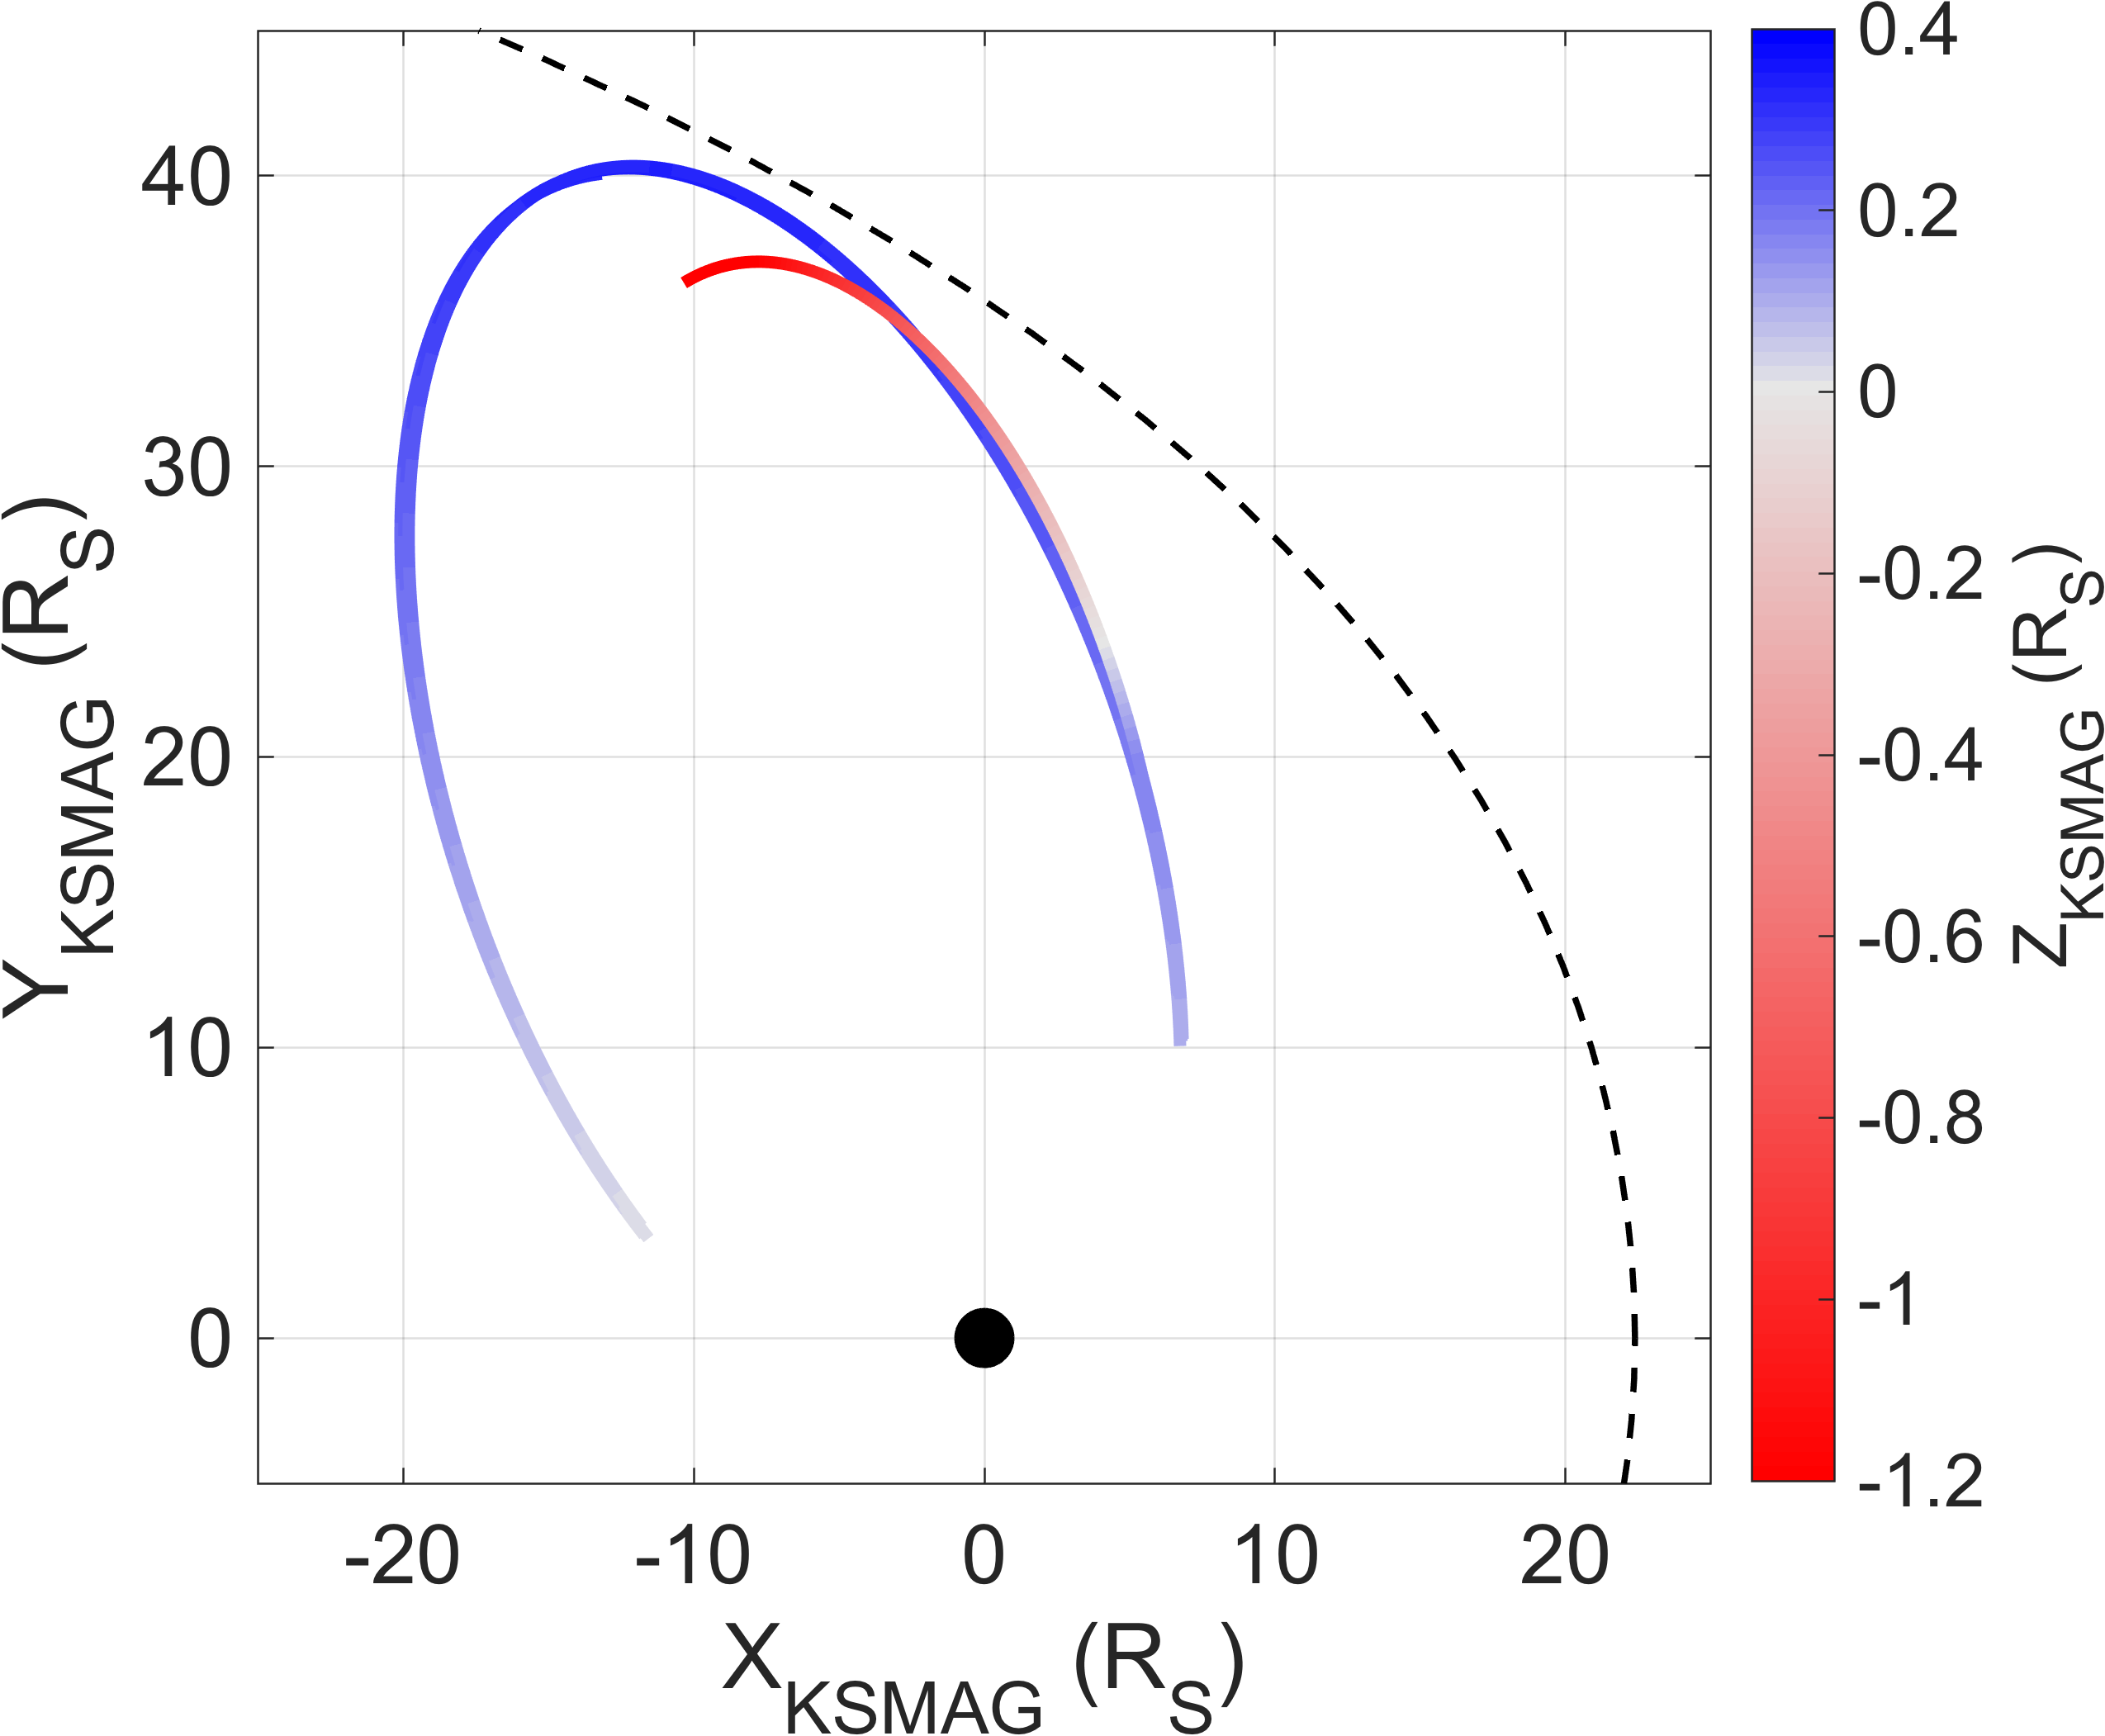
\includegraphics[width=0.7\textwidth]{equinox/cassinitrajectory.png}
% when using dvips, use .eps file:
% \includegraphics[width=20pc]{figsamp.eps}
\caption[\textit{Cassini} spacecraft trajectory for 23 October – 17 December 2009.]{The \textit{Cassini} spacecraft trajectory for the period 23 October{\--}17 December 2009 (Revs 120{\--}122), with an anticlockwise orbit. colourbar shows height above and below Saturn's rotational/dipole equator. A typical model magnetopause surface from \citet{pilkington2015} is shown by the black dashed line.}
\label{equinox:fig:cassinitrajectory}
\end{figure}

\subsection{Current Sheet Surface Model}\label{equinox:sec:cssmodel}
To model the changing location of Saturn's equatorial current sheet over time, we used a structural model first applied to Saturn by \citet{arridge2011}, simplified to exclude the aforementioned bowl-like deformation associated with solstice conditions. The approach in that study was itself a continuation of analogous studies of Jupiter's magnetodisc \citep[e.g.][]{kivelson1978,khurana2005}. The model describes a current sheet effectively tilted from the rotational equator by an angle $\theta_\mathrm{T}$ beyond a cylindrical radial distance $\rho_0$, such that the height of the current sheet above the rotational equator $z_\mathrm{CS}$ is described by
\begin{equation}\label{equinox:eq:zcs}
z_\mathrm{CS} = \tan(\theta_\mathrm{T})(\rho-\rho_0)\cos(\lambda-\lambda_0)
\end{equation}
for $\rho > \rho_0$, where $\rho_0$ is a scale length in cylindrical radial distance which controls the amplitude of the perturbation. We used $\rho_0 = \SI{12}{R_S}$ in this study, in line with previous results from \citet{southwood2007} and \citet{arridge2011}, which suggested that this type of behaviour only becomes significant beyond the magnetic shells of field-aligned currents, as discussed in Section~\ref{equinox:sec:intro}. $\lambda$ is an effective phase of this rotating perturbation, related to Saturn longitude $\lambda_\mathrm{MS}$ by
\begin{equation}\label{equinox:eq:lambda}
\lambda = \lambda_\mathrm{MS} - (\rho-\rho_0)\Omega_\mathrm{S}/v_\mathrm{W},
\end{equation}
such that the tilted current sheet pattern rotates at a rate close to the planetary rotation rate. For $\lambda_\mathrm{MS}$ we use the magnetic longitude system of \citet{andrews2012}, based on the magnetic field perturbation signal observed specifically in the Southern hemisphere, ($\Psi_\mathrm{S}$ in Figure~\ref{equinox:fig:CowleyTDdiagrams}), as this signal was at a similar or greater amplitude than the northern magnetic field perturbation signal for the period studied here \citep{andrews2012}. However we do consider the phase difference between the northern and southern signals when interpreting our results, later in this study. $\lambda_0$ is an offset parameter which describes the `phase front' of the maximum vertical displacement of the current sheet from the rotational equator relative to $\lambda$, which is equivalent to the magnetospheric longitude $\lambda_\mathrm{MS}$ at the distance $\rho = \rho_0$. $\lambda_0$ is thus effectively a `prime meridian' for this perturbation. The second term in equation~\ref{equinox:eq:lambda} introduces a radial delay in this perturbation, to account for the time taken for the magnetic perturbation to propagate radially outwards from its source, at an effective wavespeed $v_\mathrm{W}$. This causes a spiral-like pattern in the elevation of the current sheet surface. $\Omega_\mathrm{S}$ is a variable angular velocity close to the planetary rotation rate, corresponding to the angular velocity of the rotating perturbation defined by the $\lambda_\mathrm{MS}$ longitude system used here. These two terms can be represented by the single delay parameter
\begin{equation}\label{equinox:eq:D}
D = \Omega_\mathrm{S}/v_\mathrm{W},
\end{equation}
where $D$ has units of $\si{\degree/R_S}$. The corresponding spiral pattern in the current sheet structure can be seen in Figure~\ref{equinox:fig:cssurfacemodel}, which shows an example model current sheet surface with typical $D$, $\theta_\mathrm{T}$ and $\rho_0$ parameters as described in the caption. Also shown is a curve of constant phase passing through the maximum $z_\mathrm{CS}$ at each radial distance, corresponding to $\lambda=\lambda_0$.
\begin{figure}
\centering
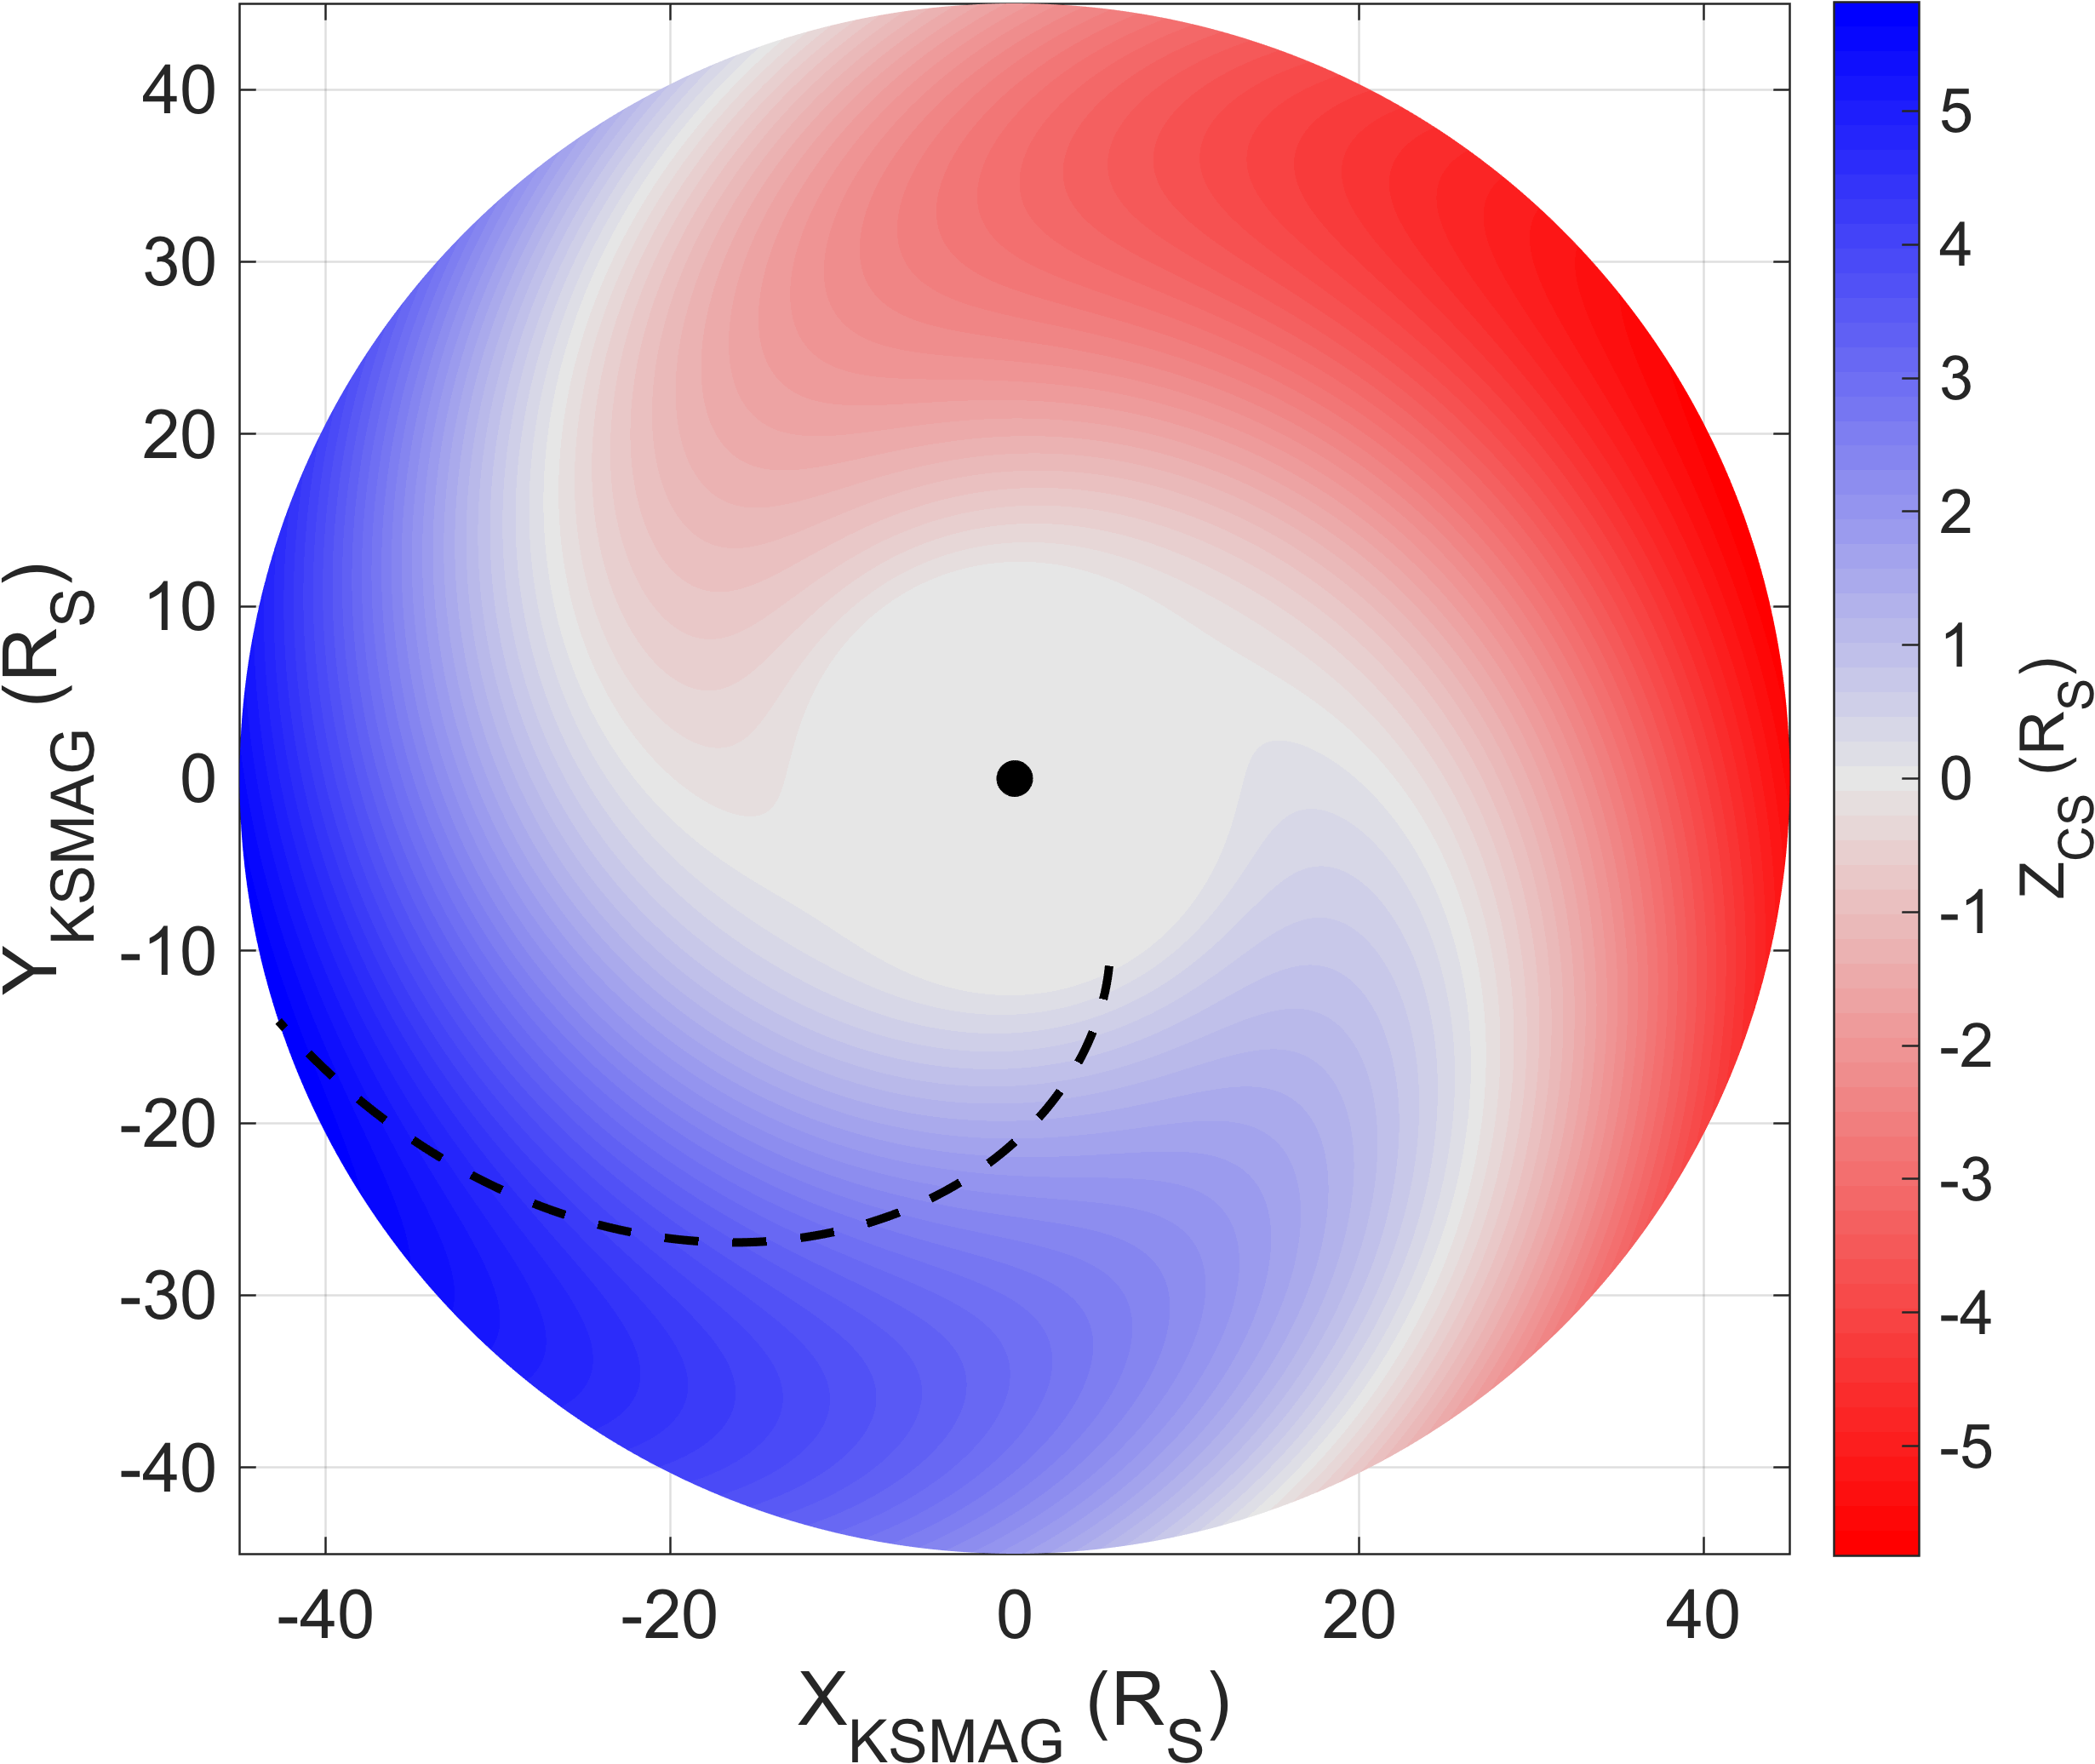
\includegraphics[width=0.7\textwidth]{equinox/cssurface.png}
% when using dvips, use .eps file:
% \includegraphics[width=20pc]{figsamp.eps}
\caption[Snapshot of tilted, rippled current sheet surface model.]{An snapshot of the current sheet surface model, with parameters $D~{=}~\SI{3}{\degree/R_S}$, $\theta_\mathrm{T}~{=}~\SI{10}{\degree}$, and $\rho_0~{=}~\SI{12}{R_S}$. Blue and red colour indicates height of the current sheet $z_\mathrm{CS}$ above and below the rotational equator. The black dashed line represents a curve of constant phase $\lambda = \lambda_0$, passing through the maximum $z_\mathrm{CS}$ at each radial distance. The whole pattern then rotates with a variable period close to that of planetary rotation.}
\label{equinox:fig:cssurfacemodel}
\end{figure}

In the original study by \citet{arridge2011} the authors found values of $D$ varying from $2.1-\SI{6.7}{\degree/R_S}$ from orbit to orbit, with an average of $\SI{3.7}{\degree/R_S}$. This is in broad agreement with the results from \citet{carbary2007}, who looked for evidence of a spiral pattern in electron intensities directly using data from \textit{Cassini's} MIMI/LEMMS instrument. They observed an average `spiral arm migration' of ${{\sim}}\SI{3.4}{\degree/R_S}$, with a range of $2.7-\SI{4.7}{\degree/R_S}$. In the study by \citet{provan2012}, the authors analyse \textit{Cassini} magnetic field data from a similar time period, to measure how the phase of the magnetic perturbations discussed in the aforementioned \citet{andrews2012} study varies with radial distance and local time, specifically for the southern perturbation. They find a roughly constant radial phase gradient of ${{\sim}}\SI{2.5}{\degree/R_S}$. On the modelling side, \citet{jiaandkivelson2012} used their MHD model of Saturn's magnetosphere with twin atmospheric vortical flows to stimulate current sheet flapping (as discussed in Section~\ref{equinox:sec:intro}), and used the modelled current sheet location at different phases and radial distances to estimate a delay of ${\sim}\SI{4.3}{\degree/R_S}$. Therefore in line with these studies, we used a value of $D = \SI{3}{\degree/R_S}$ here, corresponding to a value $v_\mathrm{W} \approx \SI{185}{\km\per\second}$.

In reality, the appropriate parameter $D = \Omega_\mathrm{S}/v_\mathrm{W}$ would vary with radial distance and local time, as the wave velocity $v_\mathrm{W}$ is dependent on plasma parameters and magnetic field strength, which vary throughout the equatorial magnetosphere. Indeed \citet{andrews2010}, using \textit{Cassini} magnetic field data estimated a radial phase speed that varied from ${\sim}\SI{150}{\km\per\second}$ on Saturn's nightside to ${\sim}\SI{500}{\km\per\second}$ on the dayside, corresponding to $D$ varying from ${\sim}3-\SI{1}{\degree/R_S}$, although they qualify that the dayside value in particular has a high uncertainty. They note that this is at least in broad agreement with estimates based on measurements presented in \citet{wilson2008} and \citet{mcandrews2009}, which suggest typical Alfv\'{e}n speeds within the equatorial ring current region of ${\sim}100-\SI{400}{\km\per\second}$, depending on magnetospheric parameters. This would correspond to a delay parameter that varies between approximately $D = 6-\SI{1}{\degree/R_S}$ (where a higher value of $D$ corresponds to a lower value of $v_\mathrm{W}$). We investigated the effect of a variation in $D$ with radial distance of this scale but found it did not significantly influence our results compared to other factors. %In addition, allowing $D$ to vary as a free parameter created a degeneracy with the parameter $\lambda_0$, as both parameters influence the phasing of the magnetic field oscillations, and meant we could not extract meaningful values for either parameter.

\subsection{Magnetic Field and Plasma Model}\label{equinox:sec:plasmamodel}
The current sheet model geometry described in the previous section must be combined with a local model of magnetic field and plasma sheet structure in order to predict magnetic field values at \textit{Cassini} locations. We geometrically `anchored' a magnetic field and plasma model to our perturbed current sheet surface model following the approach of \citet{achilleos2014}, described in that study and repeated below. For  our magnetic field and plasma model, we used a modified version of the the UCL/AGA model described in Section~\ref{intro:sec:forcebalancemodel} of this thesis. This model assumes a single mean ion mass along a given magnetic field line, which means that it cannot account for fine structural variation in magnetodisc thickness caused by the concentration of the heavier water ions towards the equatorial plane \citep[e.g.][]{persoon2009, nemeth2011}; other limitations are discussed in detail in \citet{achilleos2010a}. However, as demonstrated in that study, and \citet{achilleos2010b, sergis2018}, the model can accurately reproduce global average trends observed in Saturn's magnetodisc. The UCL/AGA model is therefore demonstrably adequate for reproducing the relatively large-scale amplitude oscillations in the magnetic field data that are analysed in this study.

We then extracted magnetic field values from this model along \textit{Cassini} trajectories to directly compare with magnetometer data. The appropriate coordinates $\rho_\mu$ and $z_\mu$ at which to sample from this model are determined for each \textit{Cassini} sampling time by the current sheet model location $z_\mathrm{CS}$, according to
\begin{align}\label{equinox:eq:coordinatetransform}
& \rho_\mu = \rho_\mathrm{S/C},\nonumber\\
& z_\mu = (z_\mathrm{S/C} - z_\mathrm{CS})\hat{\boldsymbol{z}}\cdot\hat{\boldsymbol{n}}
\end{align}
where the subscript S/C refers to the \textit{Cassini} spacecraft's actual location, $\hat{\boldsymbol{z}}$ is the unit vector along the rotation / dipole axis, and $\hat{\boldsymbol{n}}$ is the unit vector normal to the model current sheet surface calculated according to equation~\ref{equinox:eq:zcs}, using $\rho = \rho_\mathrm{S/C}$ and the $\lambda$ value of the spacecraft location at that time.

The vector components of the magnetic field perturbation (total magnetic field minus the internal dipole) $\Delta B_i$ extracted from the model at these coordinates are then transformed back to give the predicted external magnetic field $\boldsymbol{B_\mathrm{ext}}$ via
\begin{equation}\label{equinox:eq:Bext}
\boldsymbol{B_\mathrm{ext}} = \Delta B_\rho \hat{\boldsymbol{\rho}}_\mathrm{CS} + \Delta B_z \hat{\boldsymbol{n}} + \Delta B_\phi \hat{\boldsymbol{\phi}}_\mathrm{CS}
\end{equation}
where
\begin{align}\label{equinox:eq:vectortransform}
& \hat{\boldsymbol{\rho}}_\mathrm{CS} = \frac{\hat{\boldsymbol{\phi}} \times \hat{\boldsymbol{n}}}{| \hat{\boldsymbol{\phi}} \times \hat{\boldsymbol{n}}|}, \nonumber\\
& \hat{\boldsymbol{\phi}}_\mathrm{CS} = \hat{\boldsymbol{n}} \times \hat{\boldsymbol{\rho}}_\mathrm{CS}
\end{align}
such that $\hat{\boldsymbol{\rho}}_\mathrm{CS}$ and $\hat{\boldsymbol{\phi}}_\mathrm{CS}$ lie in the local tangent plane of the model current sheet surface, while $\hat{\boldsymbol{\phi}}$ is in the direction of planetary corotation. As the UCL/AGA model is purely poloidal we used $\Delta B_\phi = -\frac{1}{2} \Delta B_\rho$ to characterise the azimuthal magnetic field line bendback, again following \citet{achilleos2014}, adapted from the approach by \citet{arridge2011}. The internal magnetic field, represented by a dipole situated at Saturn's centre, is  then added to this external field to give the total magnetic field at that location. 

This formulation effectively assumes that the local magnetodisc structure at \textit{Cassini's} location may be approximated by the azimuthally symmetric UCL/AGA plasma and magnetic field model, but with the equatorial plane of this model rotated to align with the local tangent plane of the model current sheet surface according to equation~\ref{equinox:eq:zcs}. More details can be found in {\citet{achilleos2014}}, who describe the transformation between the `model coordinates' used in the computation of the model field, and a local system of coordinates defined by the tangential plane of that part of the current sheet close to the spacecraft.

\subsubsection{Model parameterisation}\label{equinox:sec:modelparamzation}
As discussed elsewhere in this thesis, the UCL/AGA model treats the plasma as consisting of a cold population, confined towards the rotational equator due to the centrifugal force exerted on it, and a hot population with associated pressure distributed uniformly along magnetic field lines. In particular the hot plasma population can  be  parameterised by a single `hot plasma index' $ K_\mathrm{H}$, where $ K_\mathrm{H}= P_\mathrm{H0}V$, the product of the equatorial hot  plasma pressure  and flux tube volume beyond a radial distance of $\SI{8}{R_S}$. In Chapter~\ref{chap:compress} we explored the effect of varying this parameter within the range $10^5{\--}10^7~\si{\pascal\meter\per\tesla}$ on the resulting magnetic field structures. In this study, we used a single value of $K_\mathrm{H} = \SI{3e6}{\pascal\m\per\tesla}$, in agreement with the corresponding \textit{in situ} observations made during the period being studied here. This is demonstrated in Figure~\ref{equinox:fig:hotpressuremodel}, which shows 10-minute-averaged hot pressure moments calculated from \textit{Cassini} MIMI data along the trajectories being studied here, and model predictions of the equatorial hot pressure profile using different $K_\mathrm{H}$ values as described in the legend. A third-order polynomial fit of the MIMI data in log-linear space is also shown, in grey, to further illustrate the agreement between the overall trend of the data and the $K_\mathrm{H} = \SI{3e6}{\pascal\m\per\tesla}$ model calculations. It should be noted that, as mentioned previously, these \textit{Cassini} trajectories are not exactly equatorial but lie within $+0.3/\SI{-1.2}{R_S}$ of the rotational equator; however, the variation in pressure associated with transient conditions is much greater than the variation associated with vertical distance from the equator for this data set, and so a comparison with the equatorial model profiles is appropriate here. We consider the potential impact of this assumption on our results in more detail in Section~\ref{equinox:sec:results}.
\begin{figure}
\centering
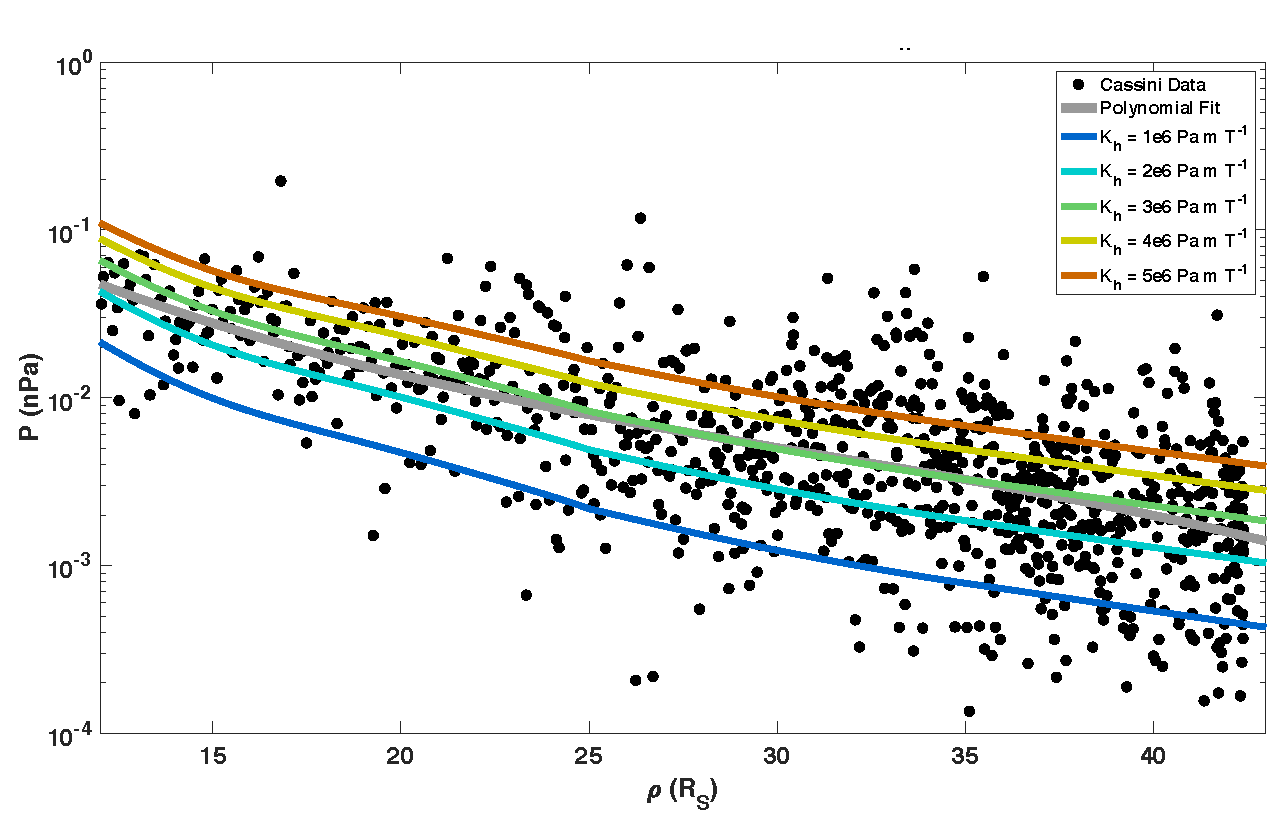
\includegraphics[width=0.9\textwidth]{equinox/hotpressuremodel.pdf}
\caption[Equatorial hot plasma pressure from \textit{Cassini} MIMI, and model predictions for different $K_\mathrm{H}$ values.]{Pressure distribution of the hot plasma population in Saturn's outer magnetosphere, against cylindrical radial distance $\rho$ in the KSMAG coordinate system. Black solid circles show 10 minute averaged hot plasma pressure moments calculated from \textit{Cassini} MIMI data along trajectories Revs 120-122, and coloured lines show equatorial model profiles using values of $K_\mathrm{H}$ as shown in the legend. The grey line shows a third-order polynomial fit of the pressure data in log-linear space, as per the axes.}
\label{equinox:fig:hotpressuremodel}
\end{figure}

The model can also be parameterised by effective magnetodisc radius $R_\mathrm{D}$, which is the cylindrical radial distance from the origin to the last closed magnetic field line, representing the location of the magnetopause boundary in the equatorial plane. A value of $\SI{45}{R_S}$ was initially used in this study, representing a typical magnetopause boundary location on the dusk flank of the magnetosphere, where \textit{Cassini} spent the majority of its time during the trajectories being studied here. This choice is discussed in more detail in Section~\ref{equinox:sec:simulatingbreathing}.

\subsubsection{Model modifications for this study}\label{equinox:sec:modmodifications}
As described in Section~\ref{intro:sec:forcebalancemodel}, the UCL/AGA model calculates the global magnetic field structure by iteratively solving a partial differential equation for the magnetic Euler potential $\alpha$, starting from a pure dipole solution and then successively perturbing it. At each iteration, a linear combination of the present solution and the previous solution is used as input for the next iteration calculation. In this study we found that, for models with particularly large disc radii, it was necessary to weight the previous solution up to four times more heavily than the present solution in order to achieve convergence, corresponding  to $\gamma=0.2$ in equation~\ref{intro:eq:convergence}.

In addition, a small uniform southward-directed `shielding field' is also added to the magnetic field perturbation at every iteration, in order to account for the magnetic field associated with the magnetopause and magnetotail current sheets. As described in Section~\ref{intro:sec:forcebalancemodel}, in the original model construction, the magnitude of this field was chosen by calculating dayside equatorial averages of the empirical field models of \citet{alexeev2005} and \citet{alexeev2006}, and the value varied with model magnetodisc radius $R_\mathrm{D}$ \citep[see][Figure 6]{achilleos2010a}. In particular the component of the shielding field associated with the magnetopause currents was based on a dipole approximation of the magnetospheric magnetic field. However in this study, we calculate magnetodisc models with large $R_\mathrm{D}$ such that the global magnetic field structure deviates significantly from a dipolar configuration, and so the magnetic moment associated with the magnetodisc ring current is large compared to the planetary dipole magnetic moment. This can be quantified as the ratio of the ring current magnetic moment to planetary dipole magnetic moment $k_\mathrm{MD} > 1$. We therefore need to also account for the contribution of the magnetodisc magnetic moment to the magnetopause current. According to \citet{alexeev2005}, the magnitude of this contribution can be approximated to the zeroth order by the field associated with the dipole magnetopause current, multiplied by the ratio $k_\mathrm{MD}$, such that the total shielding field component associated with magnetopause currents is enhanced by the factor $(1+k_\mathrm{MD})$. Therefore in this study, for `large' models with $R_\mathrm{D} > \SI{30}{R_S}$ we modify the shielding field in this way, using an extrapolation of an empirical fit to \textit{Cassini} MAG data from \citet{bunce2007} to estimate $k_\mathrm{MD}$ for each magnetodisc radius. For example, for a model with $R_\mathrm{D} = \SI{40}{R_S}$, we use $k_\mathrm{MD}{\approx}1.3$ and find that this modification enhances the total shielding field in the southward direction by ${\sim}\SI{0.3}{nT}$. We found that a change of this order does not significantly affect the global magnetic field structure, but does improve the tendency for models with more extreme disc radii to achieve convergence.

The equatorial profile of plasma angular velocity $\omega$ is a boundary condition for this model, and was updated in this study to better represent the plasma behaviour, particularly in the outer magnetosphere. The original profile was a sixth-order polynomial fit to azimuthal velocity measurements from studies by \citet{kane2008}, who used MIMI/INCA data, and \citet{wilson2008}, who used CAPS/IMS data. We used more recent azimuthal velocity measurements from the study by \citet{wilson2017}, converted to angular velocities as a fraction of corotation using a planetary rotation rate $\Omega_S = \SI{1.6185e-4}{\radian\per\second}$ ($\SI{10.7833}{\hour}$ period). In \citet{wilson2017} the authors employed a more comprehensive CAPS data set, and an improved fitting technique, to derive median and upper/lower quartile values for equatorial azimuthal velocity in $\SI{0.5}{R_S}$ radial bins between 5.5 and $\SI{30}{R_S}$. We fit the median values of median azimuthal velocities with a fourth-order polynomial, with each point weighted by the error (assumed to be half of the interquartile range), to construct an equatorial angular velocity profile. Coefficients of this polynomial are provided in the Appendix,~\ref{appendix:sec:plasmaomega}, along  with a comparison of the original profile from \citet{achilleos2010a}. For a model with $R_\mathrm{D} = \SI{45}{R_S}$, we found that this profile slightly increased the total equatorial magnetic field strength in the inner and middle magnetosphere, and slightly decreased the equatorial magnetic field strength in the outer magnetosphere, being equal at around $\rho\approx\SI{35}{R_S}$. The most extreme difference from the original magnetic field strength profile was ${\sim}\SI{1.3}{nT}$ at around $\rho\approx\SI{15}{R_S}$. This equatorial profile was then used to calculate $\omega$ throughout the model space, as $\omega$ is assumed constant along magnetic field lines in this model, in line with Ferraro's isorotation theorem; more details can be found in {\citet{achilleos2010a,caudal1986}}.

\subsection{Simulating the Breathing behaviour}\label{equinox:sec:simulatingbreathing}
As described in Section~\ref{equinox:sec:intro}, Saturn's magnetospheric current sheet is observed to not only periodically flap above and below the rotational equator, but also to periodically thicken and thin (`breathing'). In this study we attempted to simulate this compressional perturbation in a novel way, by modulating the magnetodisc radius $R_\mathrm{D}$ of the magnetic field and plasma model we sample from, depending on longitude. This is a departure from the study by {\citet{achilleos2014}}; those authors used a single UCL/AGA magnetodisc model with a fixed value of $R_\mathrm{D}$ at all azimuths, and hence did not include the periodic modulation of the current sheet thickness in their model construction. In general a model with a larger disc radius has a thinner, more distended current sheet, with magnetic field lines more `stretched out' in the radial direction, due to force balance mainly between the magnetic tension and centrifugal forces \citep{achilleos2010a,sorba2017}. In contrast a model with a relatively small disc radius has a more dipolar magnetic field structure, with more compressed field lines, and a correspondingly thicker current sheet.

We used a maximum value for $R_\mathrm{D}$ at a phase of the perturbation determined by $\lambda_\mathrm{B}$, and a minimum value at the opposite phase $\lambda_\mathrm{B}+\SI{180}{\degree}$. We varied this harmonically such that the appropriate $R_\mathrm{D}$ to use at any phase $\lambda$ determined by equation~\ref{equinox:eq:lambda} is given by
\begin{equation}\label{equinox:eq:RD}
R_\mathrm{D} = \frac{1}{2}[ R_\mathrm{MAX}+R_\mathrm{MIN}+(R_\mathrm{MAX}-R_\mathrm{MIN})\cos{(\lambda - \lambda_\mathrm{B})}].
\end{equation}
$\lambda_B$ is therefore an offset parameter for the breathing perturbation, a `prime meridian' just as $\lambda_0$ is for the flapping perturbation. It is used to describe the phase of the maximum equatorial displacement of the magnetopause boundary, and therefore thinnest current sheet, and is measured relative to $\lambda$, which is equivalent to $\lambda_\mathrm{MS}$ at $\rho=\rho_0$. The entire breathing-related perturbation then follows a spiral pattern with radial distance due to the radial delay in the perturbation propagation, as for the flapping perturbation (see equation~\ref{equinox:eq:lambda}).

This approach is illustrated in Figure \ref{equinox:fig:harmonicRD}. Panel (a) shows how the model disc radius $R_\mathrm{D}$ (shown by the solid black line) varies in $\lambda$ phase space according to equation~\ref{equinox:eq:RD}, using values $R_\mathrm{MIN}=\SI{45}{R_S}$ and $R_\mathrm{MAX}=\SI{55}{R_S}$. It can be seen that the largest disc radius is used at $\lambda=\lambda_\mathrm{B}$, and the smallest at $\lambda=\lambda_\mathrm{B}+\SI{180}{\degree}$. Panel (b) shows how this then translates into real space for a given moment in time, with colour representing which magnetodisc model radius $R_\mathrm{D}$ is used at each location.
\begin{figure}
\centering
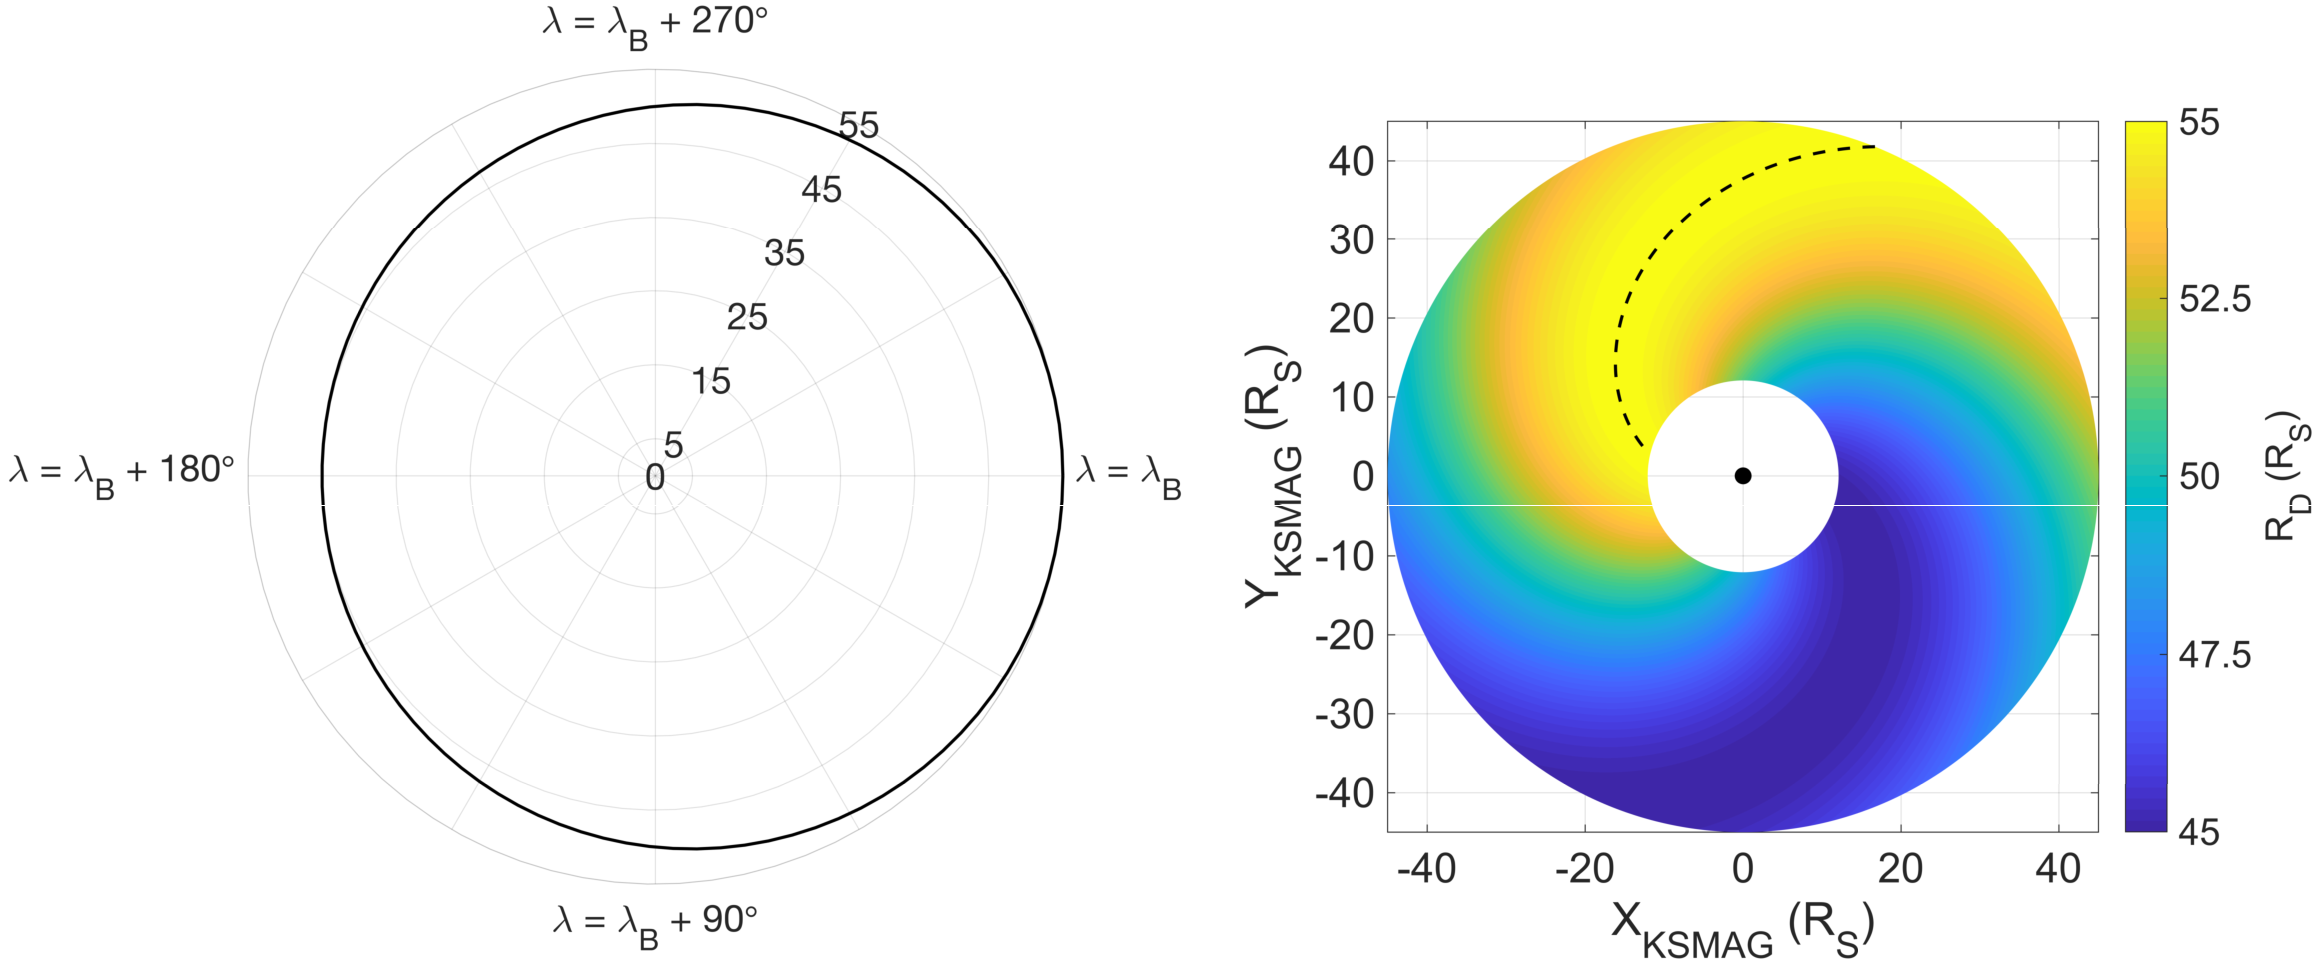
\includegraphics[width=1\textwidth]{equinox/harmonicRD.pdf}
\caption[Diagram showing how magnetodisc model radius $R_\mathrm{D}$ varies with phase, to represent breathing.]{(a) How the magnetodisc model radius $R_\mathrm{D}$ varies with phase $\lambda$, according to equation~\ref{equinox:eq:RD}. Black solid line shows $R_\mathrm{D}$, grey circles labeled with numbers from 0-55 show radius in units of $\si{R_S}$. (b) Translation of pattern (a) into real space at a given moment in time, according to $\lambda$ as described by equation~\ref{equinox:eq:lambda}. colour shows magnetodisc model radius $R_\mathrm{D}$ used at each location. The black dashed line highlights where $\lambda=\lambda_\mathrm{B}$, and hence a `breathing prime meridian' where the largest disc radius is used.}
\label{equinox:fig:harmonicRD}
\end{figure}

To determine appropriate values of $R_\mathrm{MIN}$ and $R_\mathrm{MAX}$, we compared the time period of \textit{Cassini} data being used in this study to the list of \textit{Cassini} magnetopause crossings provided by \citet{pilkington2015}. In particular, we found a period of 5 days (8 - 12 November 2009) where 24 magnetopause crossings were observed in very quick succession, each separated by only a few hours. As discussed in more detail in \citet{pilkington2015}, this suggests that the magnetopause was likely to be close to equilibrium over this time period, as otherwise only a small number of crossings would be observed as the magnetopause boundary moved rapidly over the spacecraft. We assume that the incident solar wind dynamic pressure was roughly constant over this time period, and that the observed perturbation in the magnetopause boundary location was at least in part due to changing internal pressure. This could potentially be associated with the compressional `breathing' magnetic perturbation that we are investigating here, and thus we use this perturbation in the magnetopause location to estimate a reasonable disc radius perturbation.

Figure~\ref{equinox:fig:crossingssurface} shows the locations of the observed magnetopause crossings in the KSM coordinate system, where $x_\mathrm{KSM}$ points towards the sun and $\rho_\mathrm{Y,ZKSM} = \sqrt(y_\mathrm{KSM}^2 + z_\mathrm{KSM}^2)$ is the perpendicular distance from this axis. Two potential magnetopause surface locations using the~\citet{pilkington2015} model are also shown, both using a value for solar wind dynamic pressure of $\SI{0.04}{nPa}$, and with a local plasma $\beta$ value of 0 for the inner model surface and 1.5 for the outer model surface, to replicate a change in boundary location due to internal pressure changes. These model surfaces were chosen to broadly encapsulate the range of magnetopause crossings in this time period, and thus estimate the corresponding variation in magnetopause radius. However it must be noted that these model surfaces do not represent unique solutions to the crossings shown here and are merely used to get an idea of the changing magnetopause location for this period.
\begin{figure}
\centering
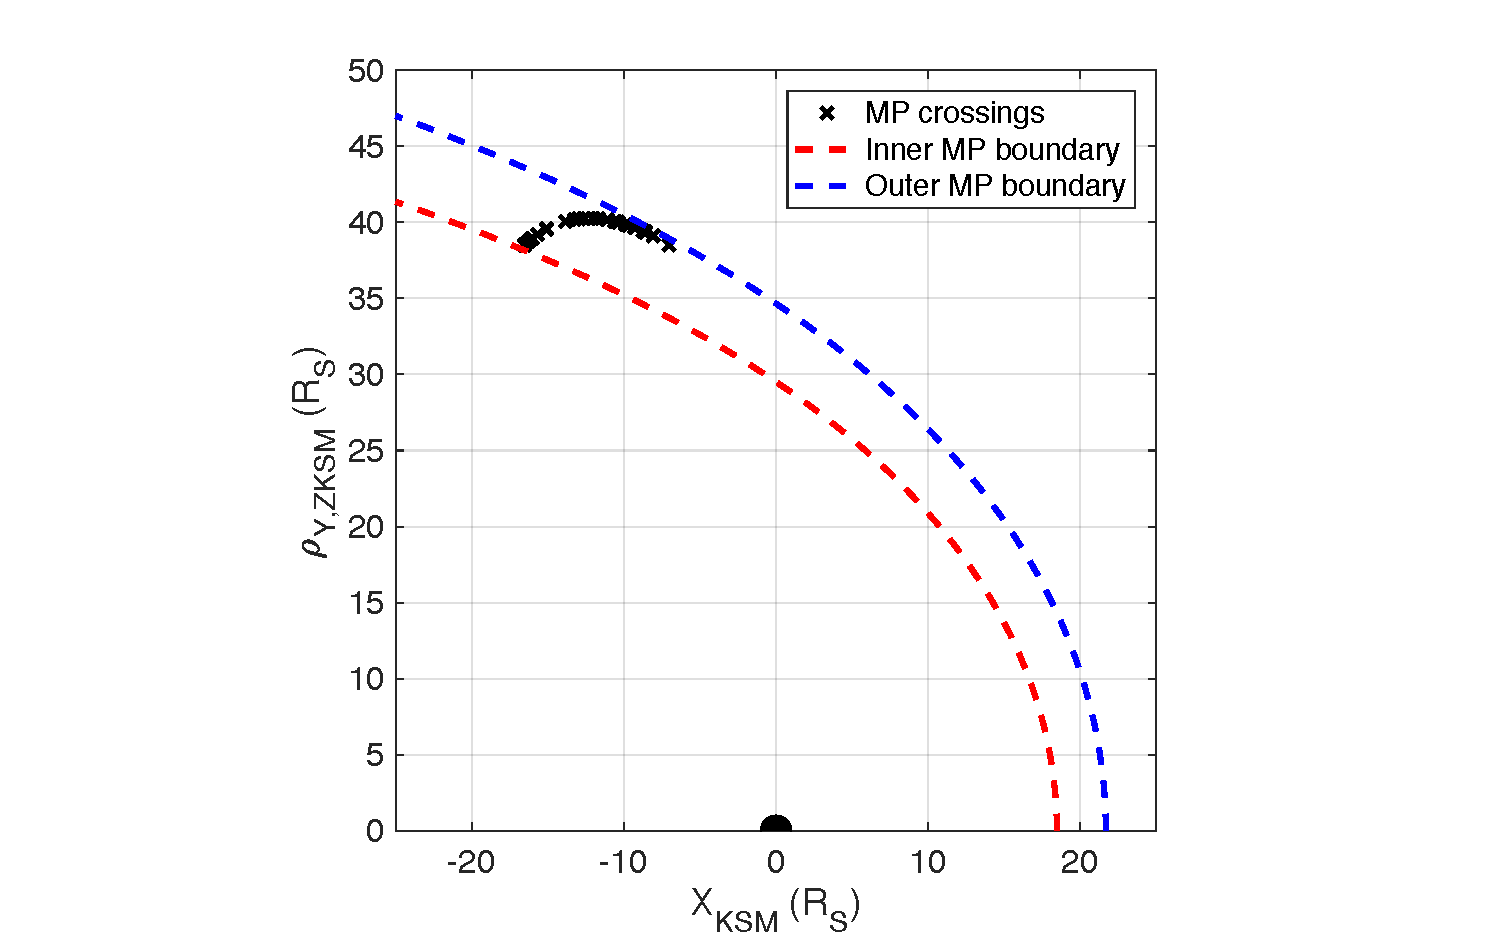
\includegraphics[width=0.6\textwidth]{equinox/crossingssurface.pdf}
\caption[Magnetopause crossings observed by \textit{Cassini}, and model magnetopause surfaces.]{Magnetopause crossings observed by \textit{Cassini} in the period 8 -12 November 2009, from \citet{pilkington2015}, in the KSM coordinate system. Model surfaces from the same study are shown in red and blue, using values for solar wind dynamic pressure and local plasma $\beta$ as described in the main text. Saturn is shown to scale at the origin by the black semicircle.}
\label{equinox:fig:crossingssurface}
\end{figure}

The difference in magnetopause radius of the two magnetopause model surfaces is $21.7-18.5 \approx\SI{3}{R_S}$ at the magnetopause nose. At the dusk flank, along the radial vector pointing from Saturn to the most anti-sunward crossing, this difference increases to $48.3-41.1\approx\SI{7}{R_S}$. A similar and even greater scale of perturbation was observed by \citet{clarke2010}, who analysed \textit{Cassini} MAG and CAPS/ELS data and found evidence that the magnetopause boundary oscillates by ${\sim}1.2{\--}\SI{5}{R_S}$ at the magnetopause nose, with a period close to the planetary rotation rate due to some internal rotating perturbation. In \citet{kivelson2014} the authors show that an MHD model that accurately predicts the current sheet flapping also produces a perturbation of ${\sim}\SI{5}{R_S}$ in the nose magnetopause location. In general a given radial perturbation in the magnetopause subsolar location corresponds to a ${\sim}2\times$ greater perturbation at the flank, using a \citet{pilkington2015} style model.

In light of these observations, and our requirement that the minimum model disc radius $R_\mathrm{D} \gtrsim \SI{44}{R_S}$ in order to provide coverage for our entire \textit{Cassini} data set, we used $R_\mathrm{MIN} = \SI{45}{R_S}$ and $R_\mathrm{MAX}=\SI{55}{R_S}$. This perturbation of $\SI{10}{R_S}$ was chosen to simulate the perturbation in the magnetopause boundary particularly on the dusk flank, where \textit{Cassini} spent most of its time for the trajectories being studied here (see Figure~\ref{equinox:fig:cassinitrajectory}). We calculated a family of five reference models with $R_\mathrm{D}$ linearly spaced in this range, and piece-wise linearly interpolated magnetic field values for the required $R_\mathrm{D}$ between them, thus assuming that the model magnetic field components at a given $\rho,z$ vary piece-wise linearly with global magnetodisc size $R_\mathrm{D}$. Figure~\ref{equinox:fig:MDALLcsthickness} (a)-(c) shows plots of how the hot plasma pressure $P_\mathrm{H}$ varies in cylindrical coordinates $\rho$ and $z$ for three of the five models we use in this study. As this quantity $P_\mathrm{H}$ is constant along magnetic field lines, this effectively shows the magnetic field structure for each of the magnetodisc models. A reference line at $z=\SI{4}{R_S}$ is included to show that for the larger magnetodisc model with $R_\mathrm{D}=\SI{55}{R_S}$, the current sheet is thinner and the magnetic field structure is more disc-like than for the models with smaller $R_\mathrm{D}$. Figure~\ref{equinox:fig:MDALLcsthickness} (d) shows equatorial magnetic field profiles for the five models used in this study. The similarity between the different profiles illustrates that our approach, of linearly interpolating between them to represent outputs from models with intermediate disc radii, is broadly appropriate here. (For comparison, a similar plot but with magnetodisc models calculated with smaller $R_\mathrm{D}$ was shown in Chapter~\ref{chap:intro}, Figure~\ref{intro:fig:MDmodels}.)

In reality, the thickness of Saturn's magnetospheric current sheet also varies with local time, with, in general, a thicker and more radially compressed current sheet on the dayside than the nightside \citep[e.g.][]{arridge2008}. In order to accurately account for this behaviour, the value of $R_\mathrm{D}$ could be also varied as a function of local time, or the family of magnetodisc models could be otherwise modified to more accurately represent different local time sectors. While non-trivial and beyond the scope of this current study, we would like to investigate this in future, and in Chapter~\ref{chap:LTsectors} we present preliminary results looking at local time variation in current sheet thickness and overall magnetodisc structure. However, for this study, our current approach is appropriate in this context and unlikely to significantly affect our conclusions. This is because we analyse each \textit{Cassini} pass individually, and the range in local time for each pass is only $\sim2-3.5$ hours, as shown by the annotations at the bottom of Figures~\ref{equinox:fig:rev120in}{\--}\ref{equinox:fig:rev122out}. This means that any variation in current sheet thickness associated with local time is likely to be less significant than the variation due to the magnetodisc breathing behaviour.
\begin{figure}
\centering
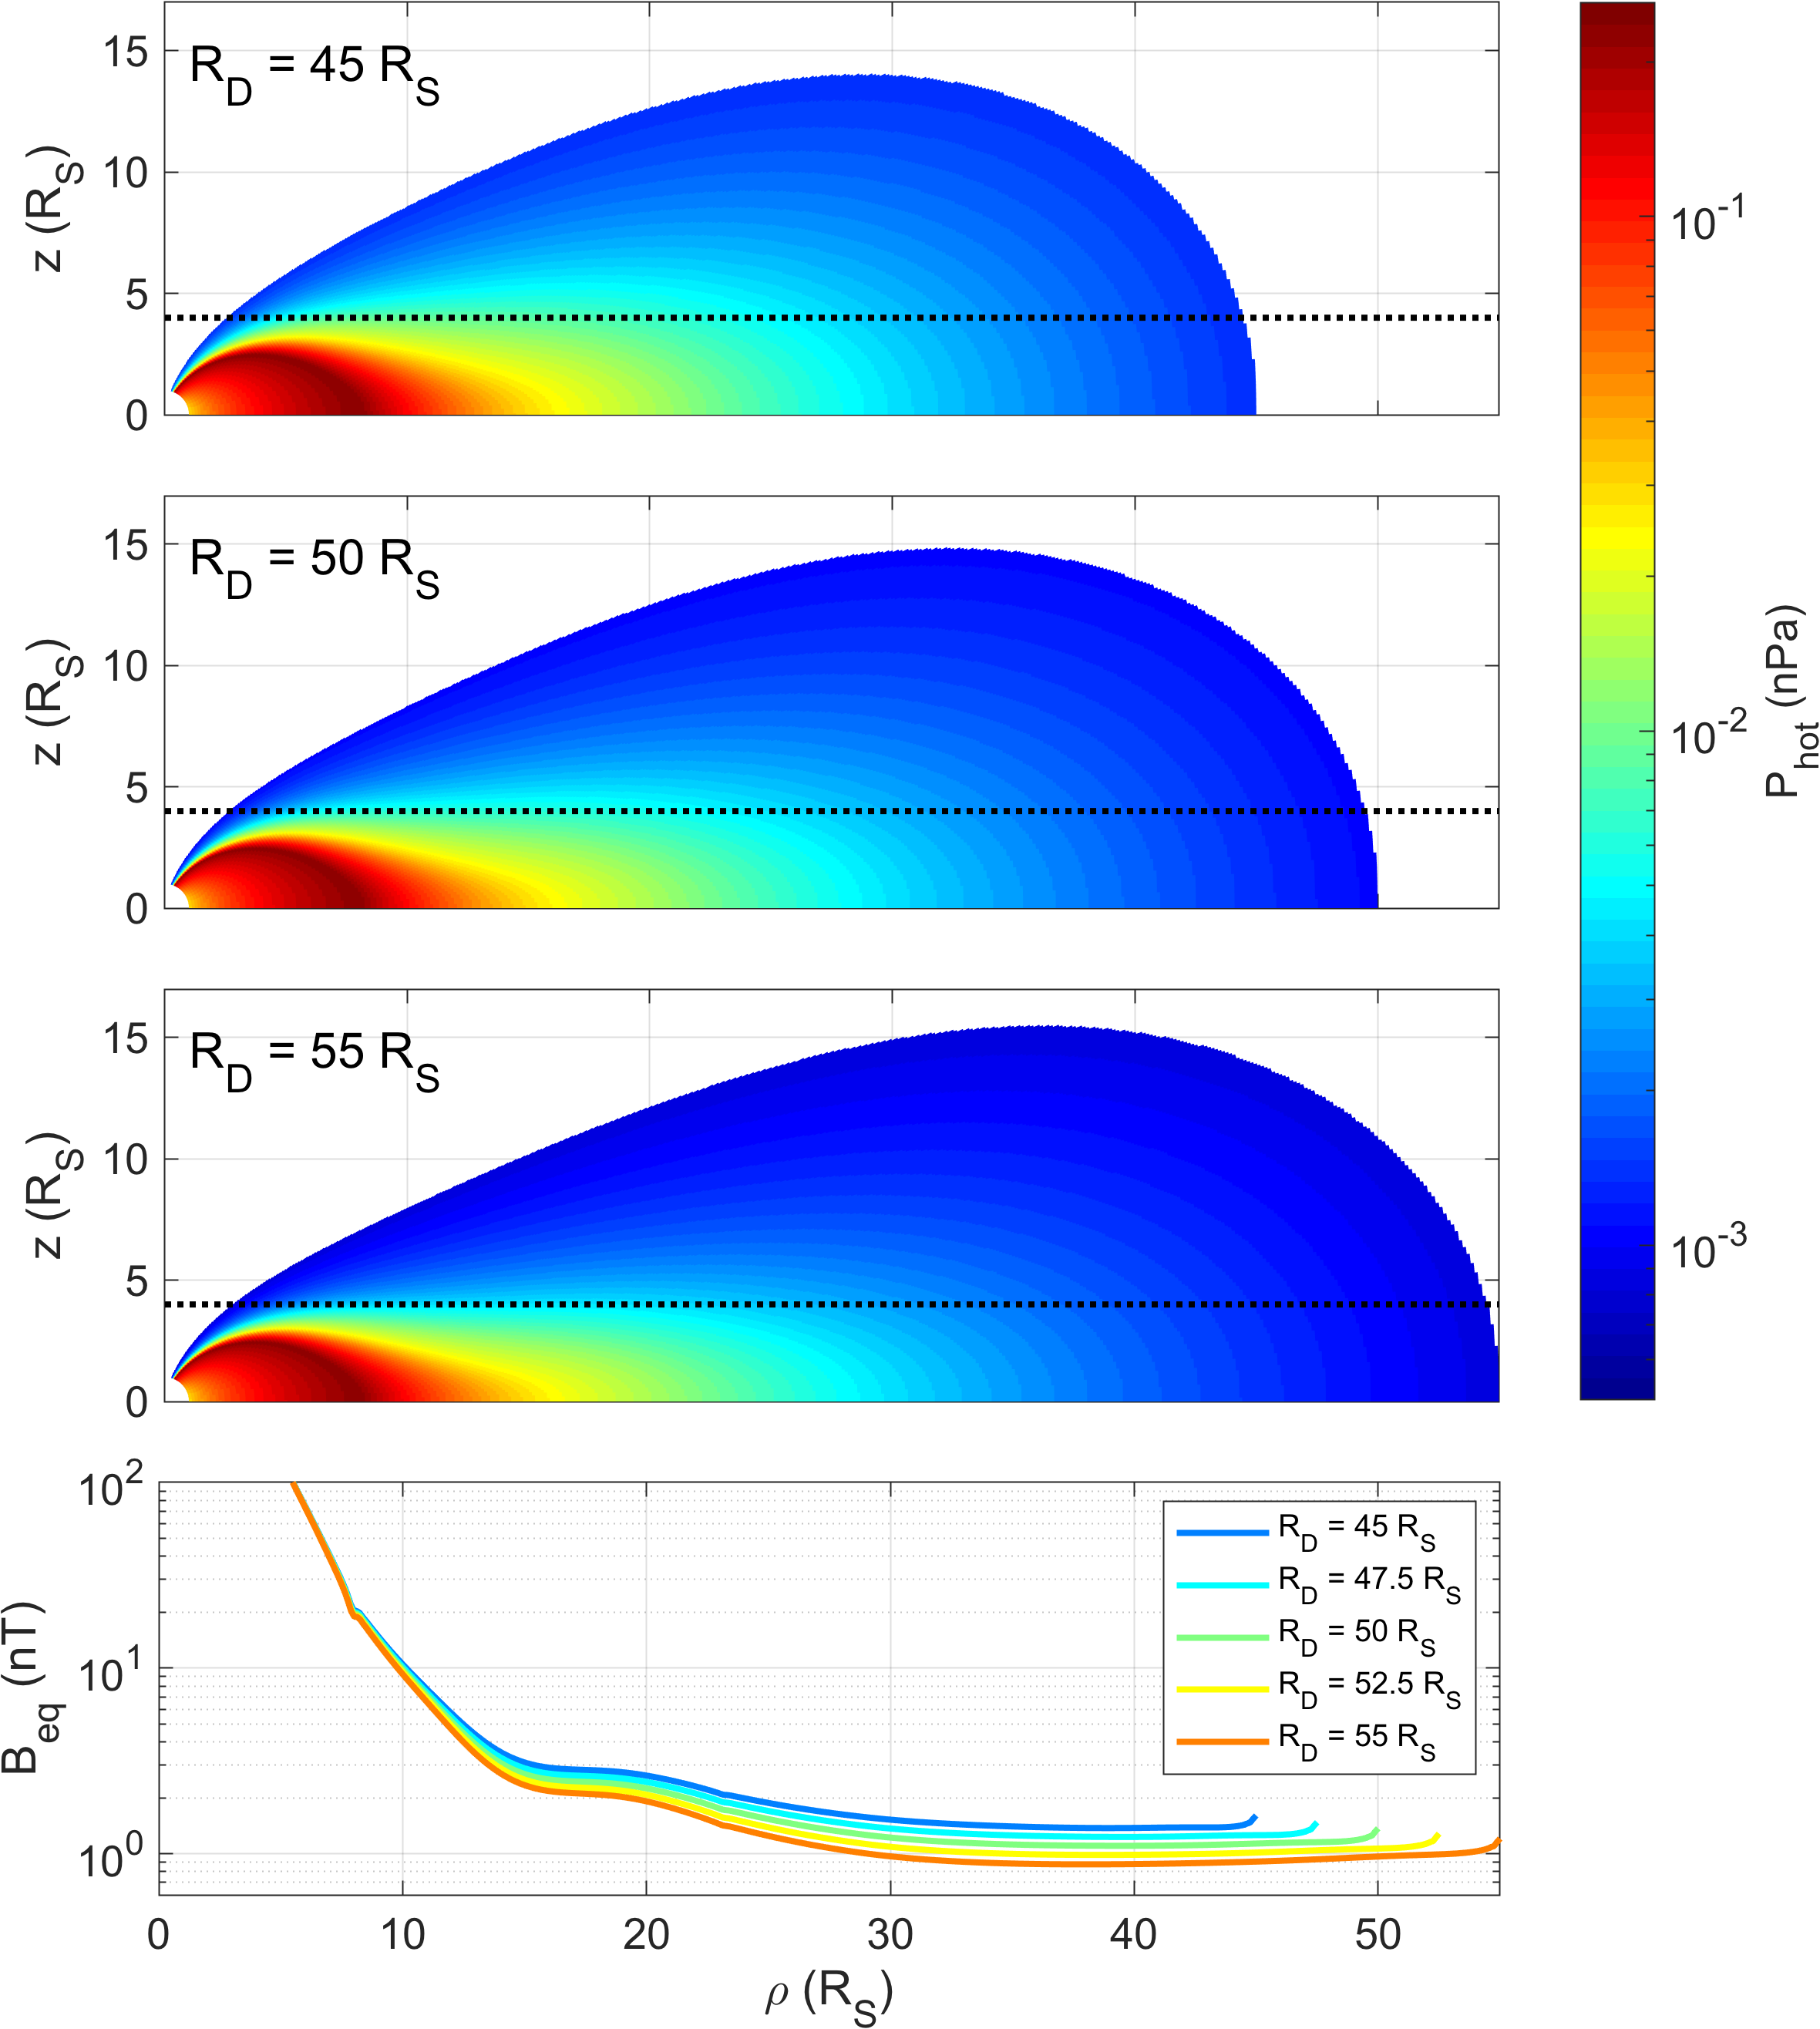
\includegraphics[width=0.7\textwidth]{equinox/MDALLcsthickness_Bfield.png}
\caption[Magnetic field structure for $R_\mathrm{D}$ = $45, 50$ and $\SI{55}{R_S}$ magnetodisc models.]{(a)-(c) Hot plasma pressure $P_\mathrm{H}$ predicted by the magnetodisc models as a function of cylindrical coordinates $\rho$ and $z$, shown on a colour scale as per the colourbar. Models calculated using model disc radii $R_\mathrm{D}$ (a) $\SI{45}{R_S}$, (b) $\SI{50}{R_S}$ and (c) $\SI{55}{R_S}$. The quantity $P_\mathrm{H}$ is constant along a given magnetic field line and thus contours are equivalent to magnetic field lines. Black dotted line at $z~{=}~\SI{4}{R_S}$ is superimposed on each plot for reference, to compare current sheet thicknesses for each model. (d) Radial profiles of equatorial magnetic field strength for each of the five models used in this study, as shown by the legend.}
\label{equinox:fig:MDALLcsthickness}
\end{figure}

\subsection{Fitting Procedure and Parameter Uncertainty Estimation}
We fit the model to all three components of the 1-hour averaged magnetic field vector data measured by \textit{Cassini} in spherical polar coordinates, with $\boldsymbol{\hat{\phi}}$ in the direction of planetary corotation, $\boldsymbol{\hat{r}}$ pointing radially away from the planet, and $\boldsymbol{\hat{\theta}}$ completing the right-handed set. We separated our \textit{Cassini} trajectories into inbound and outbound passes, and fit the current sheet model parameters relevant for each pass. For the `flapping only' model, we use a fixed magnetodisc radius $R_\mathrm{D} = \SI{45}{R_S}$ and fit the parameters $\theta_\mathrm{T}$ and $\lambda_0$, and for the `flapping and breathing' model we use a range of disc radii as described above, and fit $\theta_\mathrm{T}$, $\lambda_0$ and $\lambda_\mathrm{B}$. We used a standard non-linear least squares fitting method, minimizing the unweighted merit function
\begin{equation}
\chi^2 = \sum\limits_{i,k}(B_{k}-\hat{B_{k}})_i^2~~~~i = 1,...,N;~k = r,\theta,\phi
\end{equation}
effectively the sum of the squared differences between the model and data magnetic field vector components, where $B_k$ is the observed and $\hat{B_k}$ is the model vector component for each of the $N$ data points. We minimised this function using the Levenberg-Marquardt algorithm, and used the square root of the diagonal elements of the resulting covariance matrix to estimate the standard error, and thus 95 percent confidence limits on the fitted parameters, following \citet{press2007}.

\section{Results and Discussion}\label{equinox:sec:results}
\subsection{Results with Flapping Only, and With Influence of Breathing}
\begin{table}
\caption[Fitted parameters for FO and F{\&}B models, for \textit{Cassini} Revs 120-122.]{Tables showing fitted parameters $\theta_\mathrm{T}$, $\lambda_0$ and $\lambda_\mathrm{B}$ for each Cassini revolution (Rev) using the flapping only (`FO') model and the flapping and breathing (`F{\&}B') model. Also shown is the root-mean-square difference (RMS) between model and data magnetic field values, and the approximate phase difference between the Southern and Northern magnetic perturbations at the centre time of each pass from \citet{andrews2012} (S-N). }\label{equinox:table:fitparams}
\centering
\begin{tabular}{l l c c c c | c}
\hline
 Rev & Model & $\theta_\mathrm{T}~(\si\degree)$& $\lambda_0~(\si\degree)$ & $\lambda_\mathrm{B}~(\si\degree)$ & RMS ($\si{nT}$) & S-N ($\si{\degree}$) \\
\hline
\multirow{2}{*}{120 IN}  		& FO  		& $17.0\pm2.4$ 	& $247\pm6$ 	& -						& 1.16 	&	\multirow{2}{*}{286}\\
  											& F{\&}B  	& $14.3\pm1.8$ 	& $244\pm6$ 	& $20\pm30$ 	& 1.06	&\\  
\multirow{2}{*}{120 OUT}	& FO 		& $5.0\pm1.3$ 		& $139\pm14$ 	& - 						& 0.82	& \multirow{2}{*}{237}\\
 											& F{\&}B 	& $3.6\pm1.0$ 		& $134\pm16$ 	& $310\pm40$ 	& 0.81 &\\ 
\multirow{2}{*}{121 IN} 		& FO 		& $7.4\pm1.8$ 		& $5\pm13$ 		& - 						& 1.19 & \multirow{2}{*}{156} \\
  											& F{\&}B 	& $6.4\pm1.4$ 		& $11\pm12$ 	& $270\pm40$	& 1.12 & \\ 
\multirow{2}{*}{121 OUT}	& FO 		& $10.4\pm2.0$ 	& $268\pm9$ 	& -						& 0.65 & \multirow{2}{*}{99}\\
											& F{\&}B 	& $8.4\pm1.2$ 		& $259\pm7$ 	& $191\pm22$ 	& 0.53 & \\ 
\multirow{2}{*}{122 IN}		& FO 		& $14.9\pm2.5$ 	& $280\pm8$	& -						& 1.27 & \multirow{2}{*}{52} \\
											& F{\&}B 	& $18.4\pm2.3$ 	& $285\pm5$ 	& $200\pm30$ &	1.16 &\\ 
\multirow{2}{*}{122 OUT}	& FO 		& $8.1\pm1.5$ 		& $205\pm10$ & -					& 0.90	& \multirow{2}{*}{10}\\
											& F{\&}B 	& $6.8\pm1.4$ 	& $202\pm11$ 	& $310\pm40$		&	0.97 &\\
\hline
%\multicolumn{2}{l}{$^{a}$Footnote text here.}
\end{tabular}
\end{table}
\begin{figure}
\centering
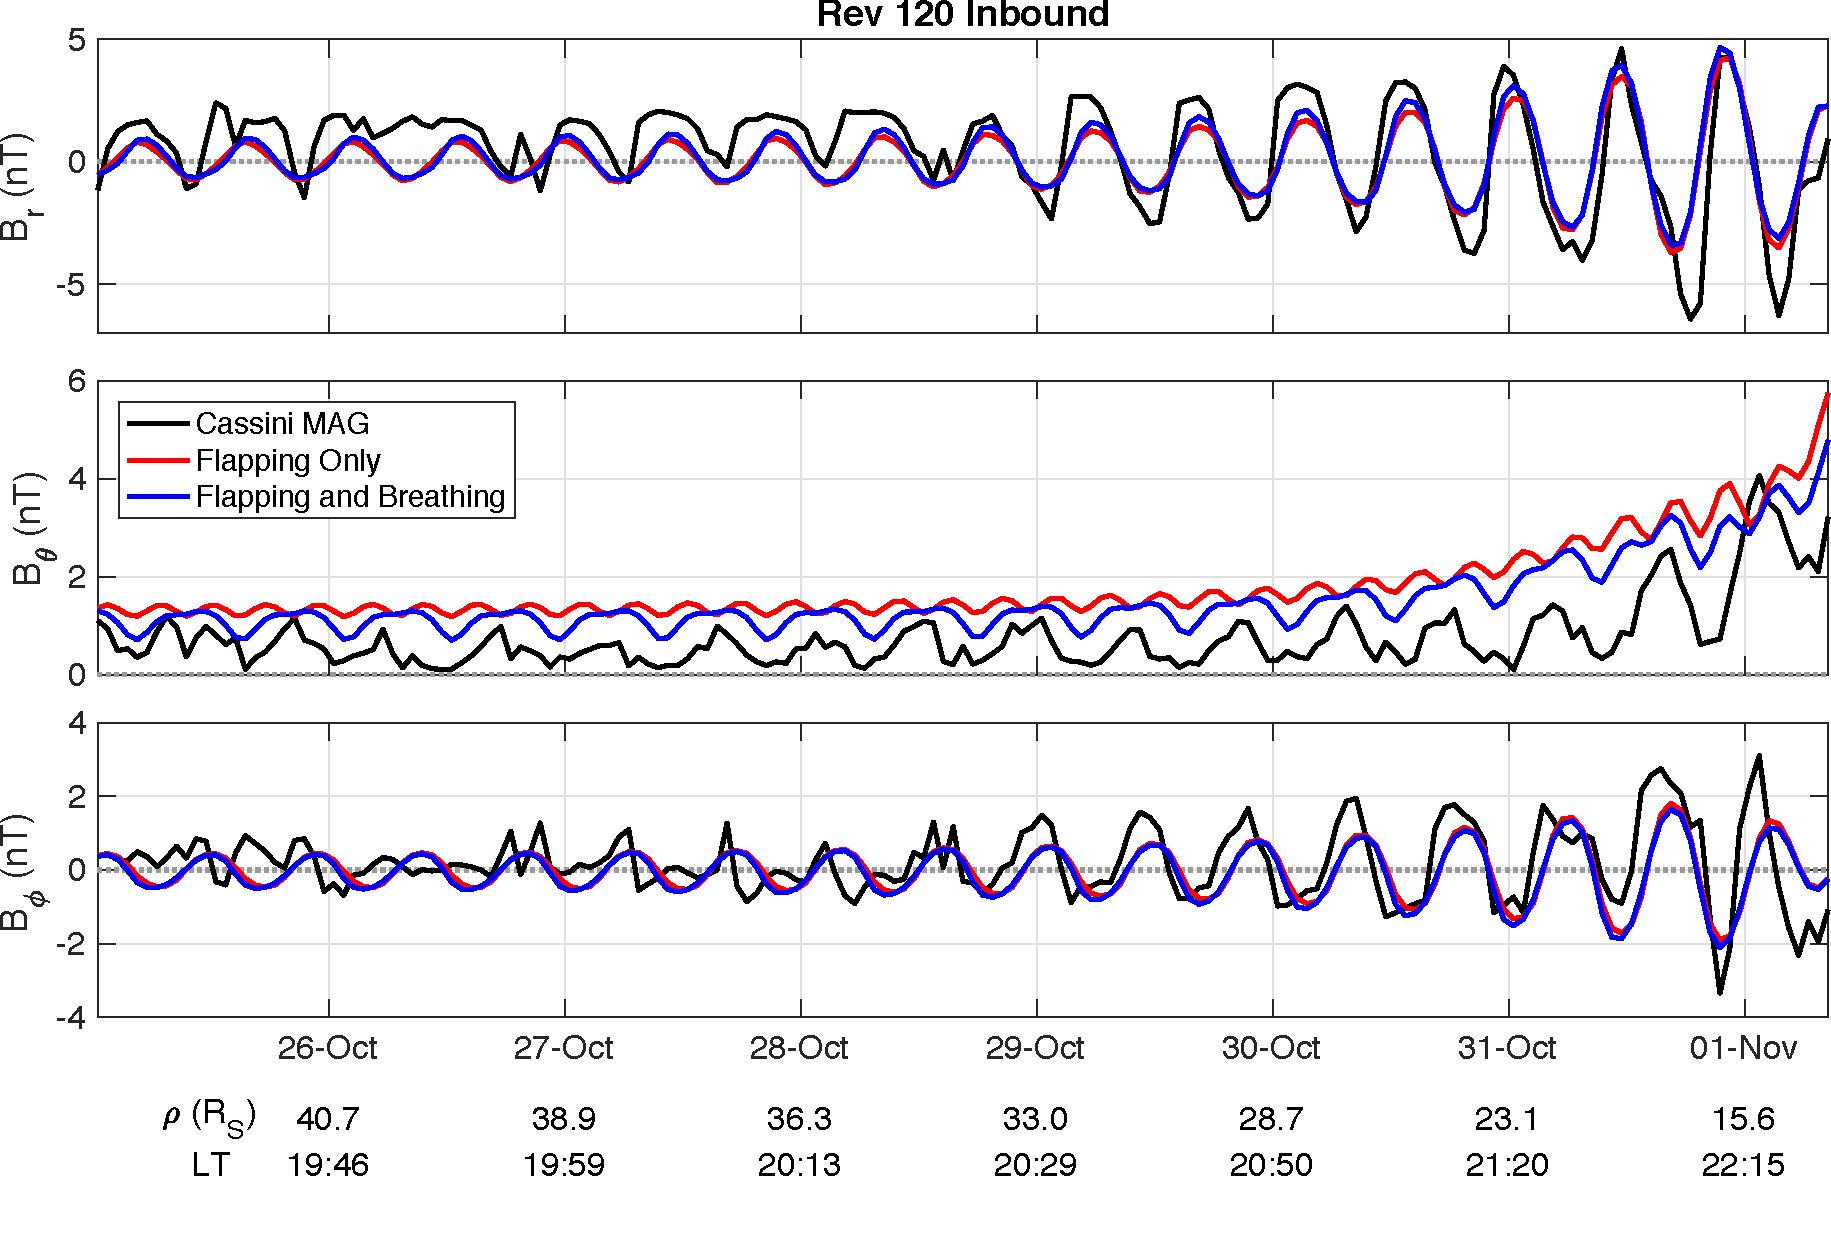
\includegraphics[width=0.9\textwidth]{equinox/rev120in.pdf}
\caption[\textit{Cassini} MAG data, FO and F{\&}B model predictions for Rev 120 Inbound.]{Radial (a), meridional (b) and azimuthal (c) components of the magnetic field measured by \textit{Cassini} along \textbf{Rev 120 Inbound}, outside of $\rho~{=}~\SI{12}{R_S}$ and inside the magnetosphere. In black we show the MAG data, in red is the flapping only model, and in blue is the flapping and breathing model, both with best fit parameters shown in Table~\ref{equinox:table:fitparams}. Annotation labels underneath give $\rho$, the cylindrical radial distance of \textit{Cassini} from the planet in KMSAG coordinates and the Saturn magnetic local time LT.}
\label{equinox:fig:rev120in}
\end{figure}
\begin{figure}
\centering
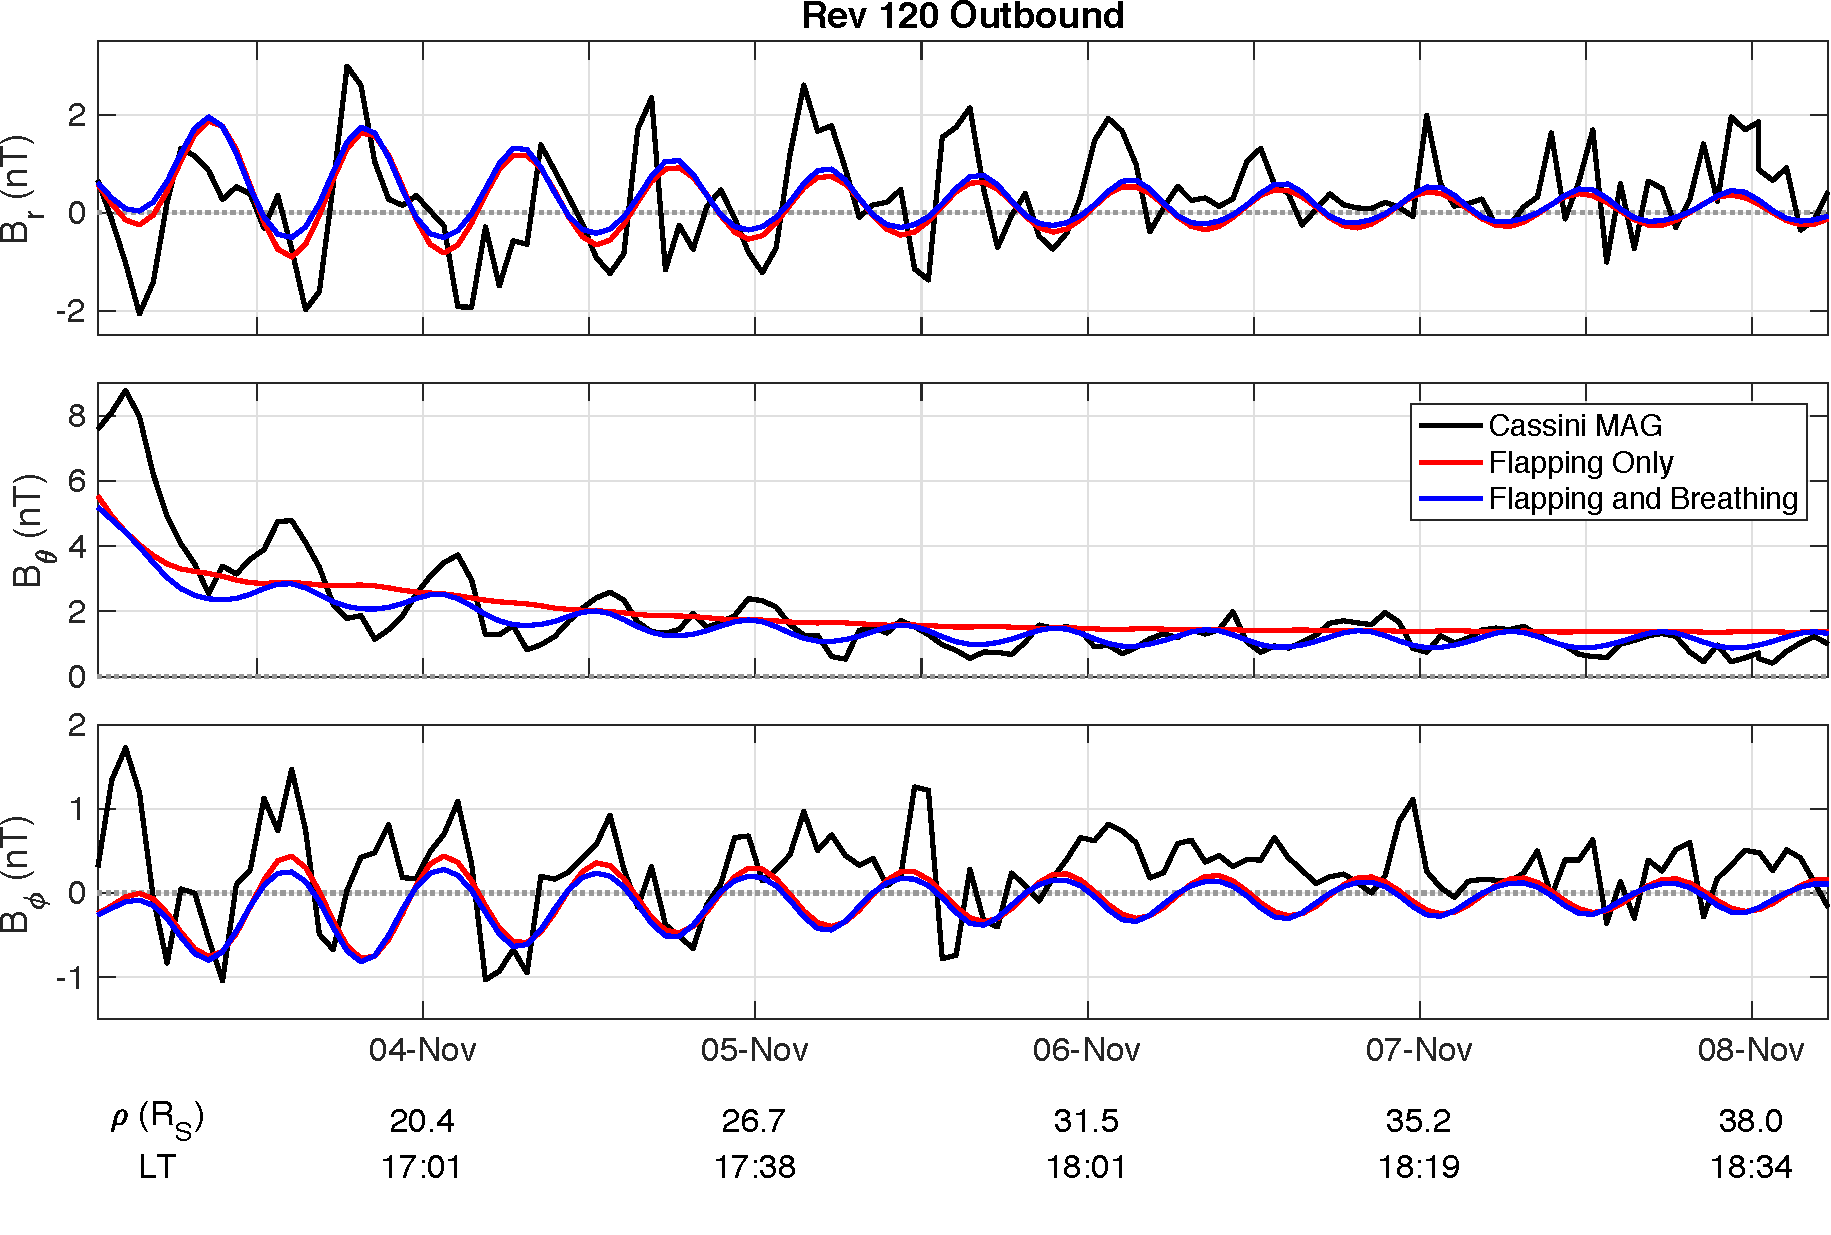
\includegraphics[width=0.9\textwidth]{equinox/rev120out.pdf}
\caption[\textit{Cassini} MAG data, FO and F{\&}B model predictions for Rev 120 Outbound.]{As for Figure~\ref{equinox:fig:rev120in} for \textbf{Rev 120 Outbound}.}
\label{equinox:fig:rev120out}
\end{figure}
\begin{figure}
\centering
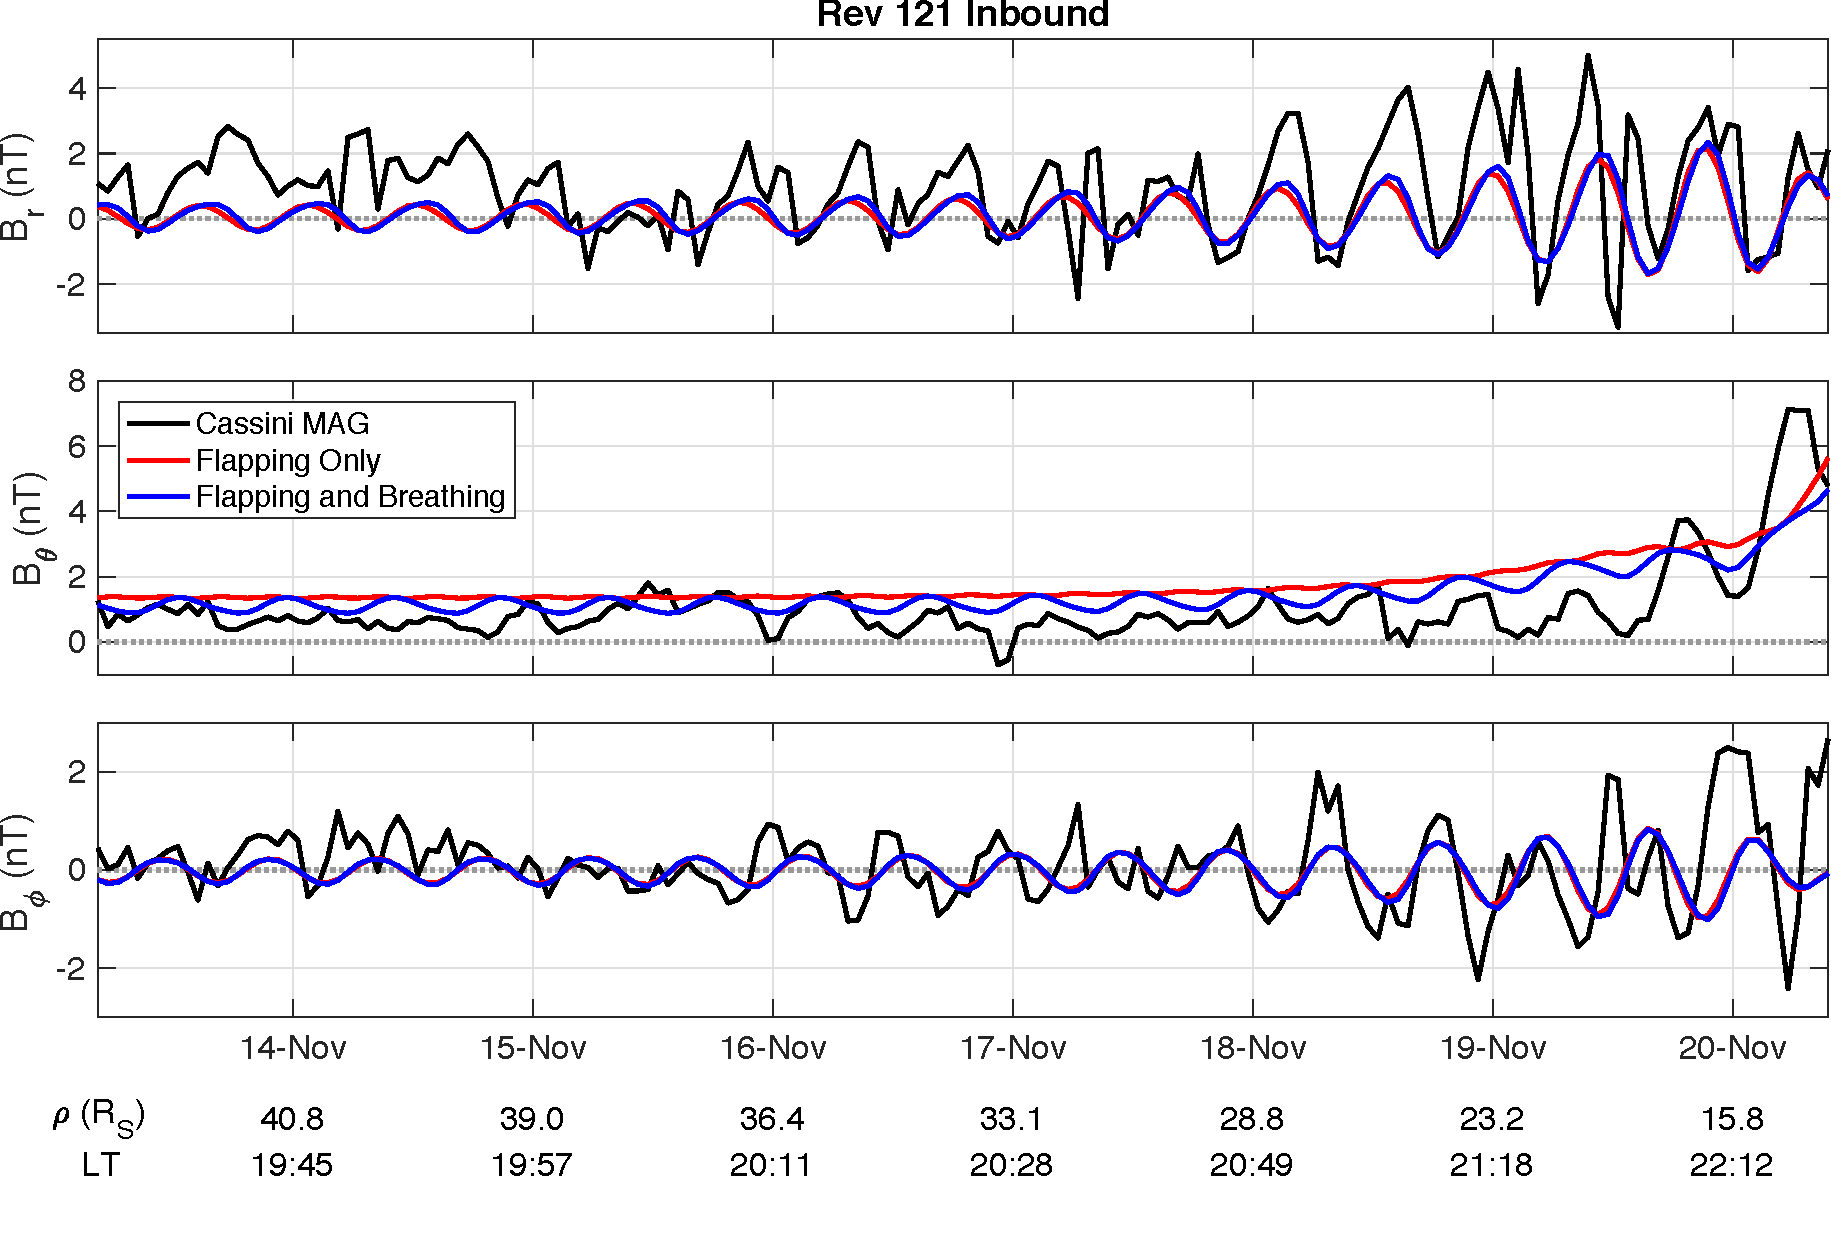
\includegraphics[width=0.9\textwidth]{equinox/rev121in.pdf}
\caption[\textit{Cassini} MAG data, FO and F{\&}B model predictions for Rev 121 Inbound.]{As for Figure~\ref{equinox:fig:rev120in} for \textbf{Rev 121 Inbound}.}
\label{equinox:fig:rev121in}
\end{figure}
\begin{figure}
\centering
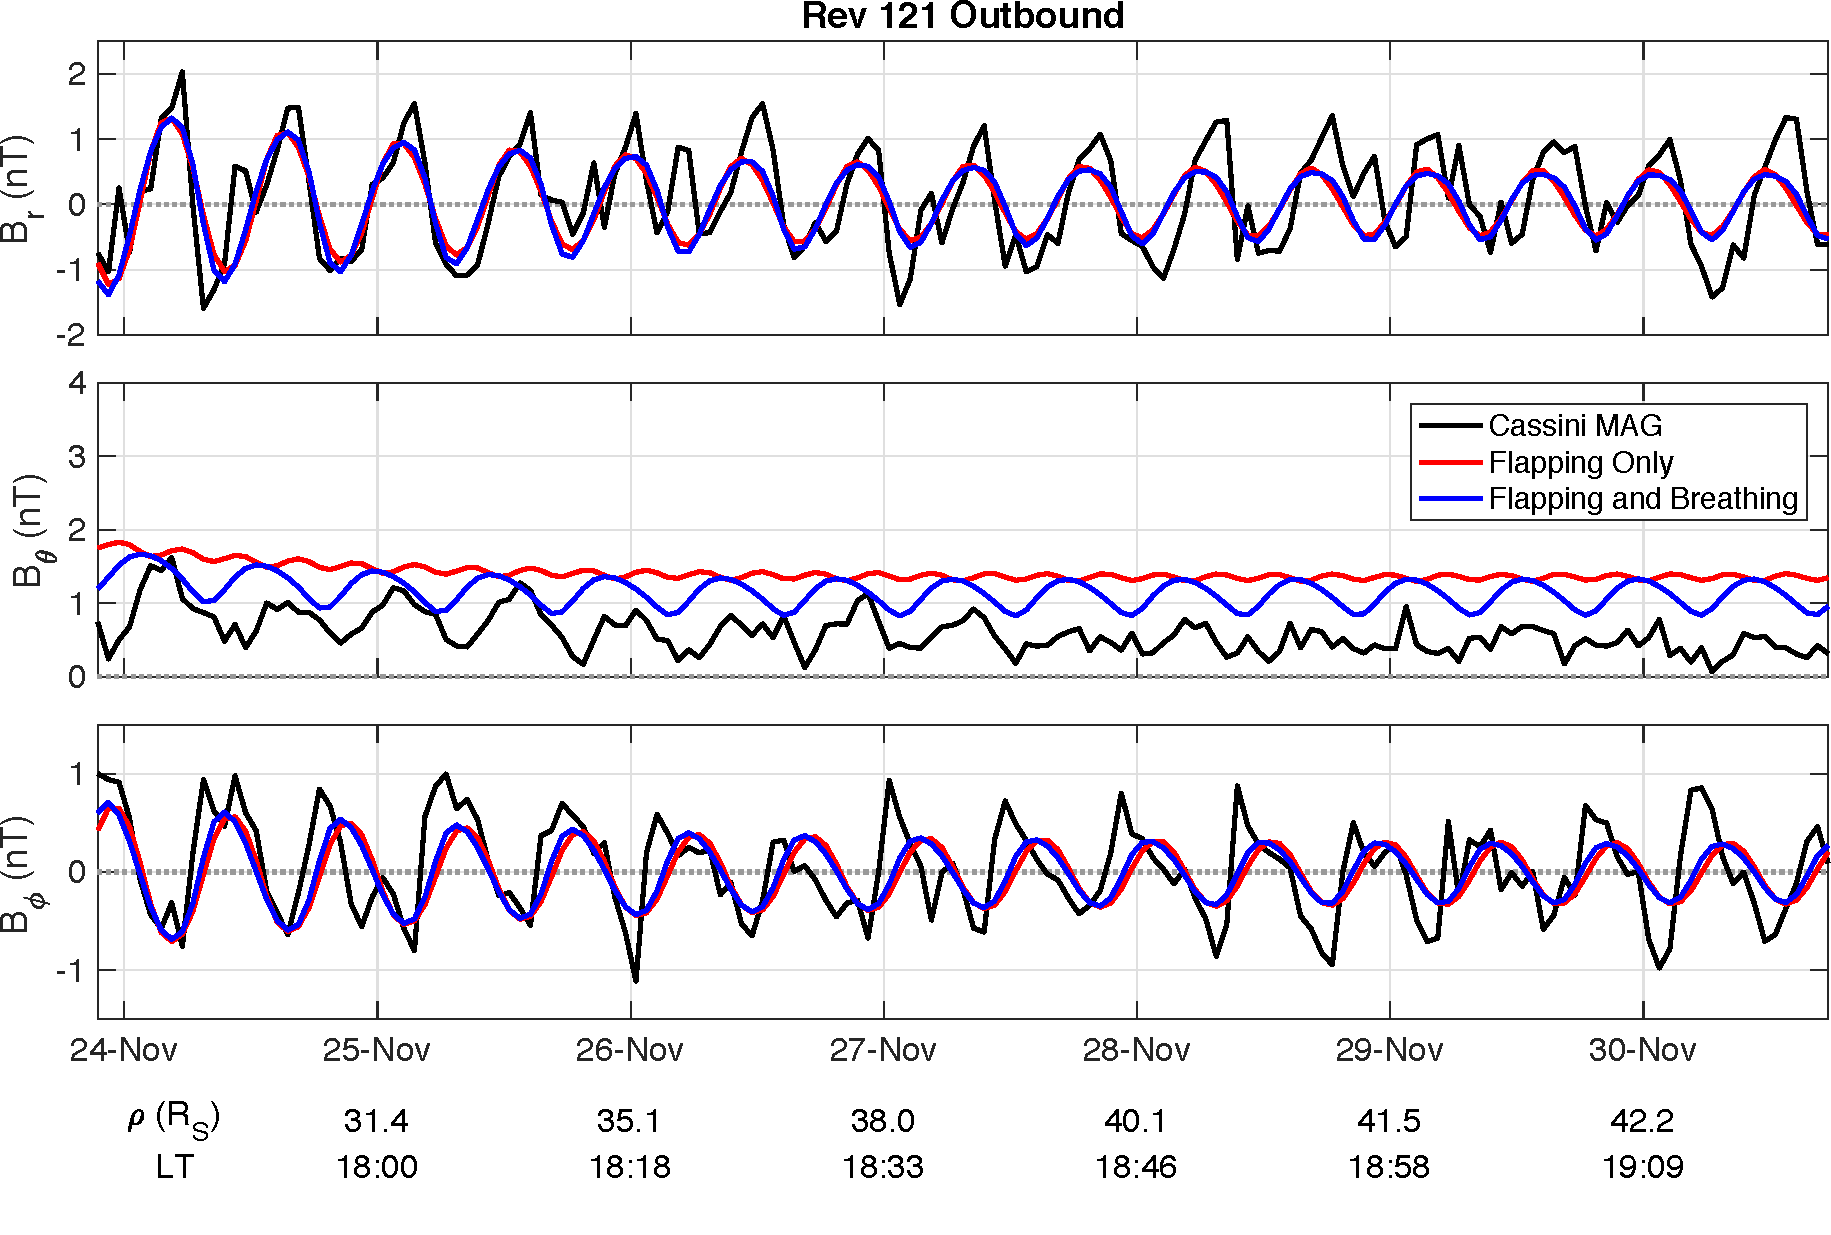
\includegraphics[width=0.9\textwidth]{equinox/rev121out.pdf}
\caption[\textit{Cassini} MAG data, FO and F{\&}B model predictions for Rev 121 Outbound.]{As for Figure~\ref{equinox:fig:rev120in} for \textbf{Rev 121 Outbound}.}
\label{equinox:fig:rev121out}
\end{figure}
\begin{figure}
\centering
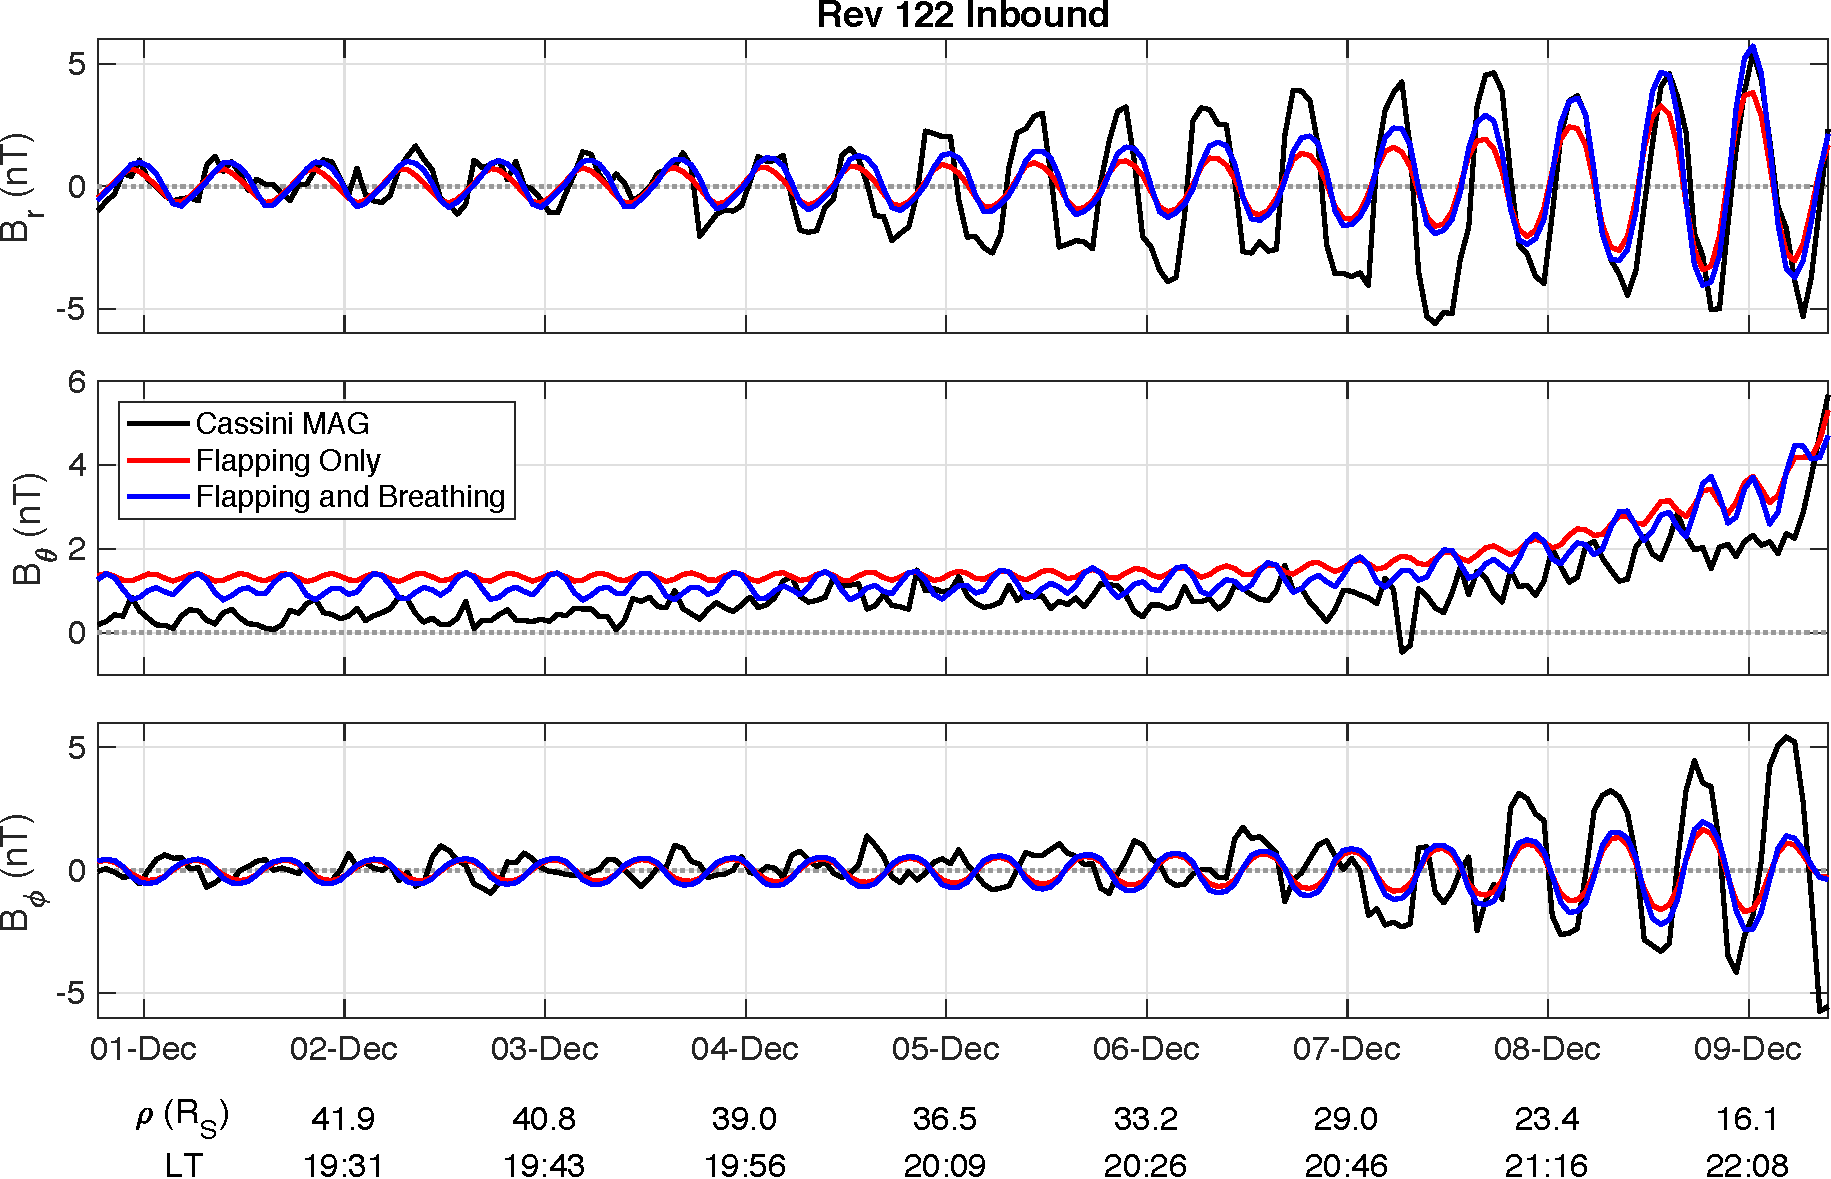
\includegraphics[width=0.9\textwidth]{equinox/rev122in.pdf}
\caption[\textit{Cassini} MAG data, FO and F{\&}B model predictions for Rev 122 Inbound.]{As for Figure~\ref{equinox:fig:rev120in} for \textbf{Rev 122 Inbound}.}
\label{equinox:fig:rev122in}
\end{figure}
\begin{figure}
\centering
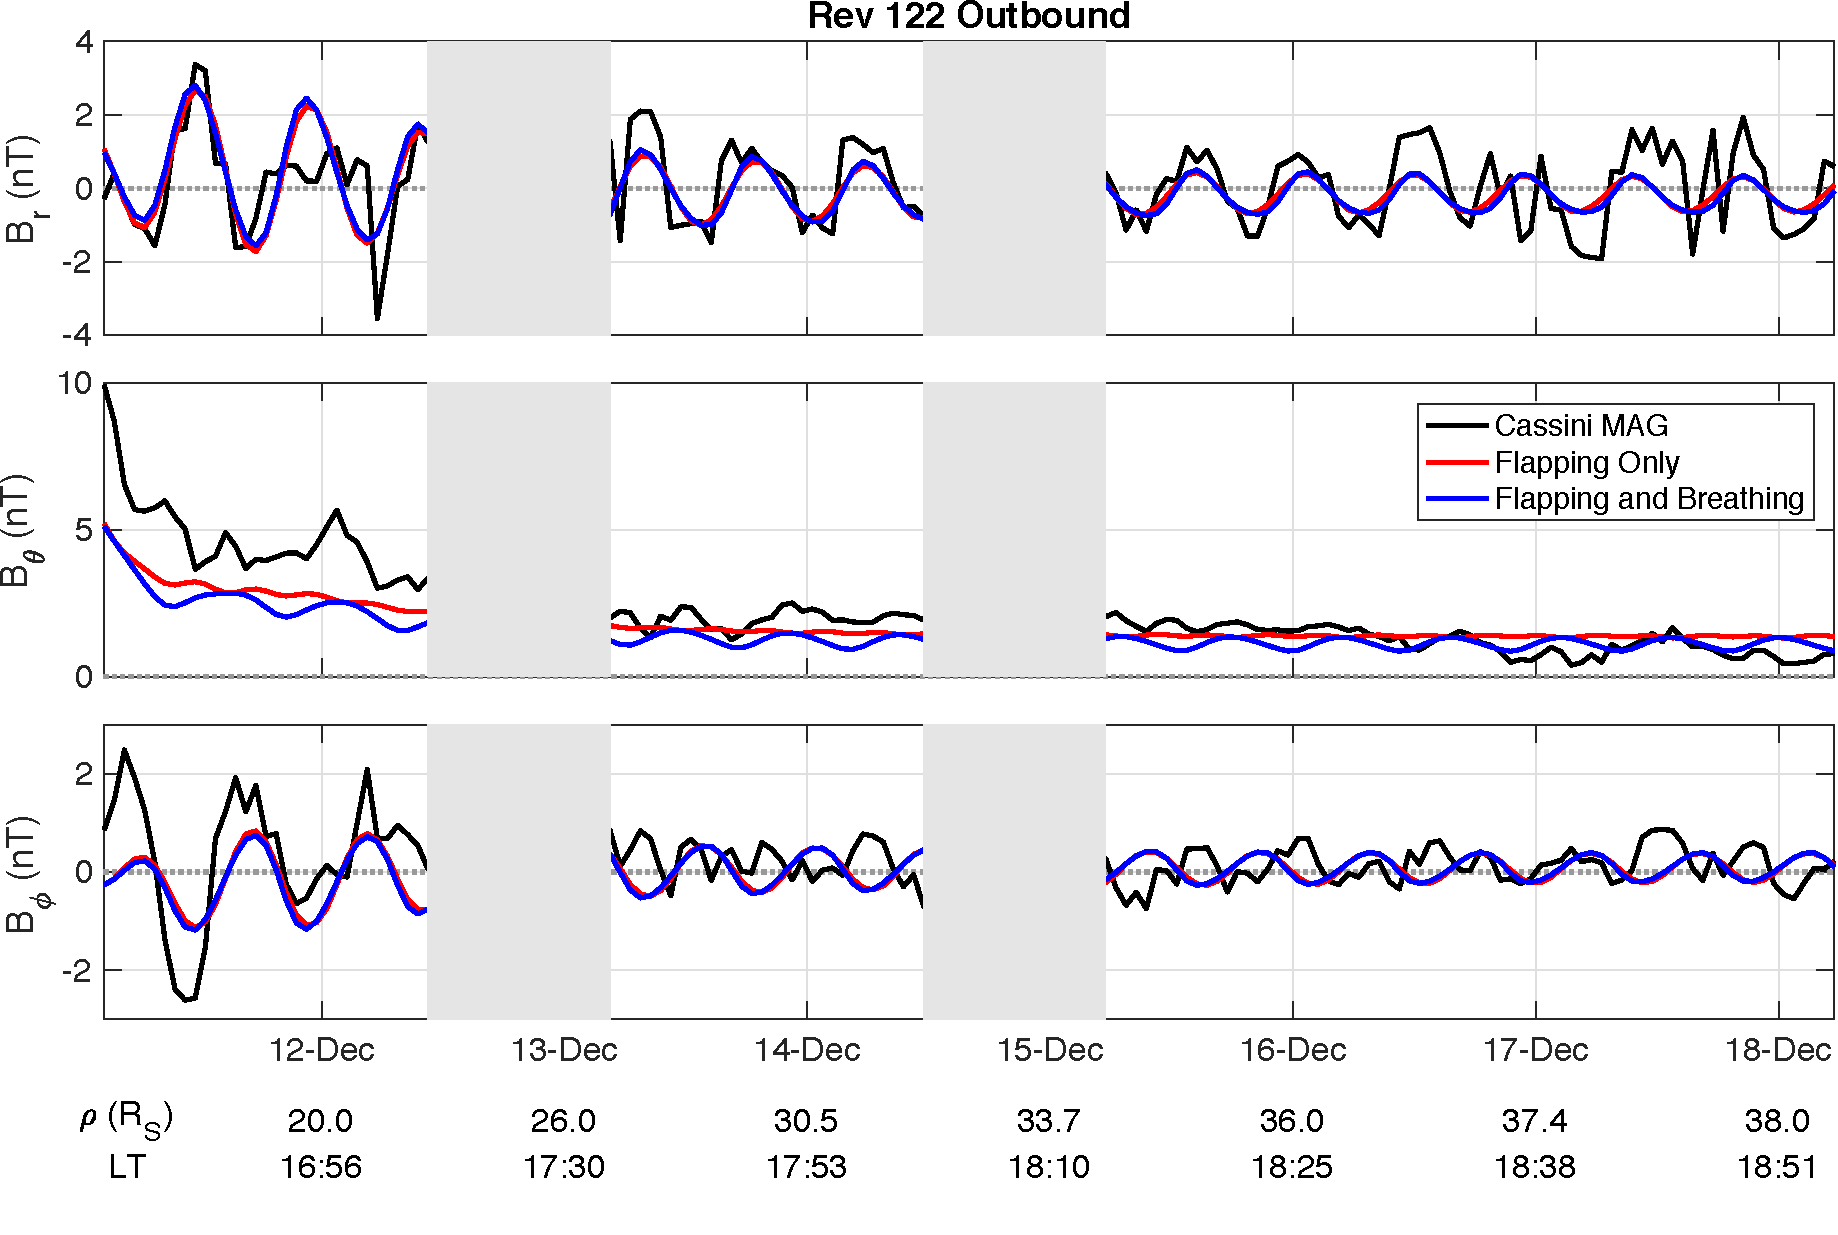
\includegraphics[width=0.9\textwidth]{equinox/rev122out.pdf}
\caption[\textit{Cassini} MAG data, FO and F{\&}B model predictions for Rev 122 Outbound.]{As for Figure~\ref{equinox:fig:rev120in} for \textbf{Rev 122 Outbound}. The grey shaded regions correspond to where \textit{Cassini} was outside of the magnetosphere and so the model was not fit to data in these regions.}
\label{equinox:fig:rev122out}
\end{figure}
Figures~\ref{equinox:fig:rev120in}~to~\ref{equinox:fig:rev122out} show the Cassini magnetic field data acquired on each pass, and the predictions by the `flapping only' and `flapping and breathing' models. The corresponding best fit parameters are shown in Table~\ref{equinox:table:fitparams}. Also shown is the root-mean-square difference (RMS) between the model and data magnetic field values for each model, equivalent to $\sqrt( \chi^2/n)$.

In general we can see that for passes that show clear periodicities in the magnetic field data, the `flapping only' (FO) model characterises these oscillations well, particularly in the radial ($B_{r}$) and azimuthal ($B_\phi$) components. This is most clearly shown in Figures~\ref{equinox:fig:rev120in} and \ref{equinox:fig:rev121out}. For all passes, the best fit values of $\theta_\mathrm{T}$ with the FO model are in broad agreement with the literature discussed in Section~\ref{equinox:sec:intro}, although with considerable variation pass to pass. Note that the y-axis scales are not exactly the same for Figures~\ref{equinox:fig:rev120in} to \ref{equinox:fig:rev122out}, and that therefore the amplitudes of the oscillations in the magnetic field data significantly vary from pass to pass. Similarly for $\lambda_0$, with the exception of Rev 121 Inbound, our values are consistent with those of \citet{arridge2011}, who found their fits for a parameter equivalent to $\lambda_0$ varied from $101{\--}\SI{292}{\degree}$ between passes.

However we can also see that in almost all passes, the FO model does not well reproduce the oscillations in the meridional ($B_{\theta}$) component. Similar discrepancies between model and data were observed in \citet{achilleos2014}, who used a similar model construction as for the FO model discussed here. (In \citet{arridge2011} the measured meridional component of the magnetic field was not compared to the model prediction.) In particular in this study, the FO model predicts a oscillation in $B_{\theta}$ of very small amplitude compared to the observations, and with a period approximately twice that of the rotation period. This can be understood as follows: in the FO model, the only source of periodicity is the vertical displacement of the current sheet, which moves across the spacecraft twice per planetary rotation, once from above the rotational equator and once from below. In this picture the $B_{r}$ and $B_{\phi}$ components are both oppositely oriented either side of the current sheet, with $B_{r}$ maximum positive above the current sheet due to the magnetodisc magnetic field structure, and $B_{\phi}$ maximum negative above the current sheet due to the bending back of magnetic field lines, due to the lag in plasma corotation. These components are then reversed when \textit{Cassini} is under the current sheet, and therefore even for the relatively simple FO model, these magnetic field components show a full oscillation roughly once per planetary rotation, in antiphase with each other. In contrast, in the FO picture, $B_{\theta}$ varies symmetrically either side of the current sheet, with a maximum at the current sheet centre and a minimum both above \textit{and} below, and hence it varies twice per planetary rotation, maintaining the same (positive) algebraic sign. For observations where \textit{Cassini's} orbit is persistently above or below the flapping current sheet, this would appear as a single oscillation in $B_{\theta}$, once per planetary rotation, with a single maximum observed when the current sheet is closest to the spacecraft. However in the trajectories being studied here, as shown in Figure~\ref{equinox:fig:cassinitrajectory}, \textit{Cassini} is orbiting extremely close to the rotational equator and thus close to the mean location of the current sheet. Therefore the current sheet flaps fully above and below the spacecraft every rotation, giving a double oscillation in the $B_{\theta}$ component.

It is for this reason that the F{\&}B model much better characterises the $B_{\theta}$ component in these instances. This is particularly clear in Figures~\ref{equinox:fig:rev120in}, \ref{equinox:fig:rev120out}, \ref{equinox:fig:rev121in} and \ref{equinox:fig:rev121out}, where the introduction of the breathing behaviour improves the characterization of both the amplitude and phase of the oscillations in $B_{\theta}$. Specifically for the phase, we now observe an oscillation in $B_{\theta}$ only approximately once per planetary rotation. In the `breathing' picture we discussed in Section~\ref{equinox:sec:intro}, this is interpreted as the `breathing in' or compression of the magnetic field lines and thickening of the current sheet at one phase of the perturbation $\lambda$, corresponding to a maximum in $B_{\theta}$, and the `breathing out' and thinning of the current sheet at the diametrically opposite phase, corresponding to a minimum in $B_{\theta}$. The phase is related to Saturn longitude as per equation~\ref{equinox:eq:lambda}, and so as the planet rotates, a stationary observer would pass through each of these longitudes once per rotation, causing a single dominant oscillation in $B_{\theta}$, as predicted by the F{\&}B model. The better agreement between this improved model and the MAG data for the passes referenced above supports the picture described in Section~\ref{equinox:sec:intro} and illustrated in Figure~\ref{equinox:fig:CowleyTDdiagrams}, that the rotating magnetic perturbations do cause a periodic modulation in the current sheet thickness as well as location. For all but Rev 122 Outbound, the F{\&}B model has a slightly lower RMS than the FO model as shown in Table~\ref{equinox:table:fitparams}, suggesting better agreement with the data, however we note that for all trajectories shown here the difference in RMS values between the FO and F\&B models is very minor.

The amplitude of the $B_{\theta}$ oscillations in the F{\&}B model is controlled by the harmonic variation in disc radius $R_\mathrm{D}=45{\--}\SI{55}{R_S}$. In some passes this amplitude appears somewhat underestimated by the model, suggesting a larger range of $R_\mathrm{D}$ and thus a larger range in current sheet thicknesses at different longitudes would be more appropriate. However we soon approach the limits of possible convergence for our magnetodisc model when using such high values of $R_\mathrm{D}$, and, as discussed in Section~\ref{equinox:sec:simulatingbreathing}, such large values for the magnetopause location would not be physically justifiable. This issue is a consequence of the model construction, as the variation in current sheet thickness in the model can only be controlled indirectly via the range in $R_\mathrm{D}$. Nevertheless, for illustration, in Figure~\ref{equinox:fig:rev121outdiffMDs} we reproduce the F{\&}B model shown in Figure~\ref{equinox:fig:rev121out}, and compare with a model using the same best fit parameters for Rev 121 Outbound, but employing a larger range of disc radii. In this illustrative model we use the original family of five magnetodisc models as described in Section~\ref{equinox:sec:simulatingbreathing}, supplemented with a larger model with $R_\mathrm{D}=\SI{65}{R_S}$, such that the total range is $\SI{20}{R_S}$. We show this comparison for Rev 121 Outbound in particular because of the approximate $\SI{90}{\degree}$ difference between the northern and southern perturbation phases, and the best-fit values for the flapping and breathing prime meridians, as shown in Table~\ref{equinox:table:fitparams}. This gives good conditions for observing the `sawtooth' signature particularly in the radial component of the magnetic field. As described in the Introduction, this signature is associated with the spacecraft traversing a thinner part of the current sheet in one part of the planetary rotation cycle, and a thicker part in the opposite part \citep{cowley2017a} and so is more prevalent when there is a more extreme variation in current sheet thickness in different hemispheres. This produces an asymmetric periodic sawtooth-like signature due to the longer time taken to traverse a thicker current sheet. 

Reassuringly, when we re-fit this new illustrative model with $\SI{20}{R_S}$ range in $R_\mathrm{D}$ to the MAG data for Rev 121 Outbound, we find that the resulting best fit parameters $\theta_\mathrm{T}$, $\lambda_0$ and $\lambda_\mathrm{B}$ are equivalent to those for our F{\&}B model for that Rev within uncertainties (although note that in Figure~\ref{equinox:fig:rev121outdiffMDs} we show the illustrative model with the exact same parameters as for our original model as shown in Table~\ref{equinox:table:fitparams}, for more direct comparison). However we can see that for the illustrative model the sawtooth signature in the radial field is indeed more pronounced, due to the more extreme range in current sheet thickness for the set of magnetodisc models used here. In addition the amplitude of oscillations in $B_{\theta}$ are greater, for the same reason. This shows the inevitable sensitivity of our results to the chosen magnetodisc model parameters.
\begin{figure}
\centering
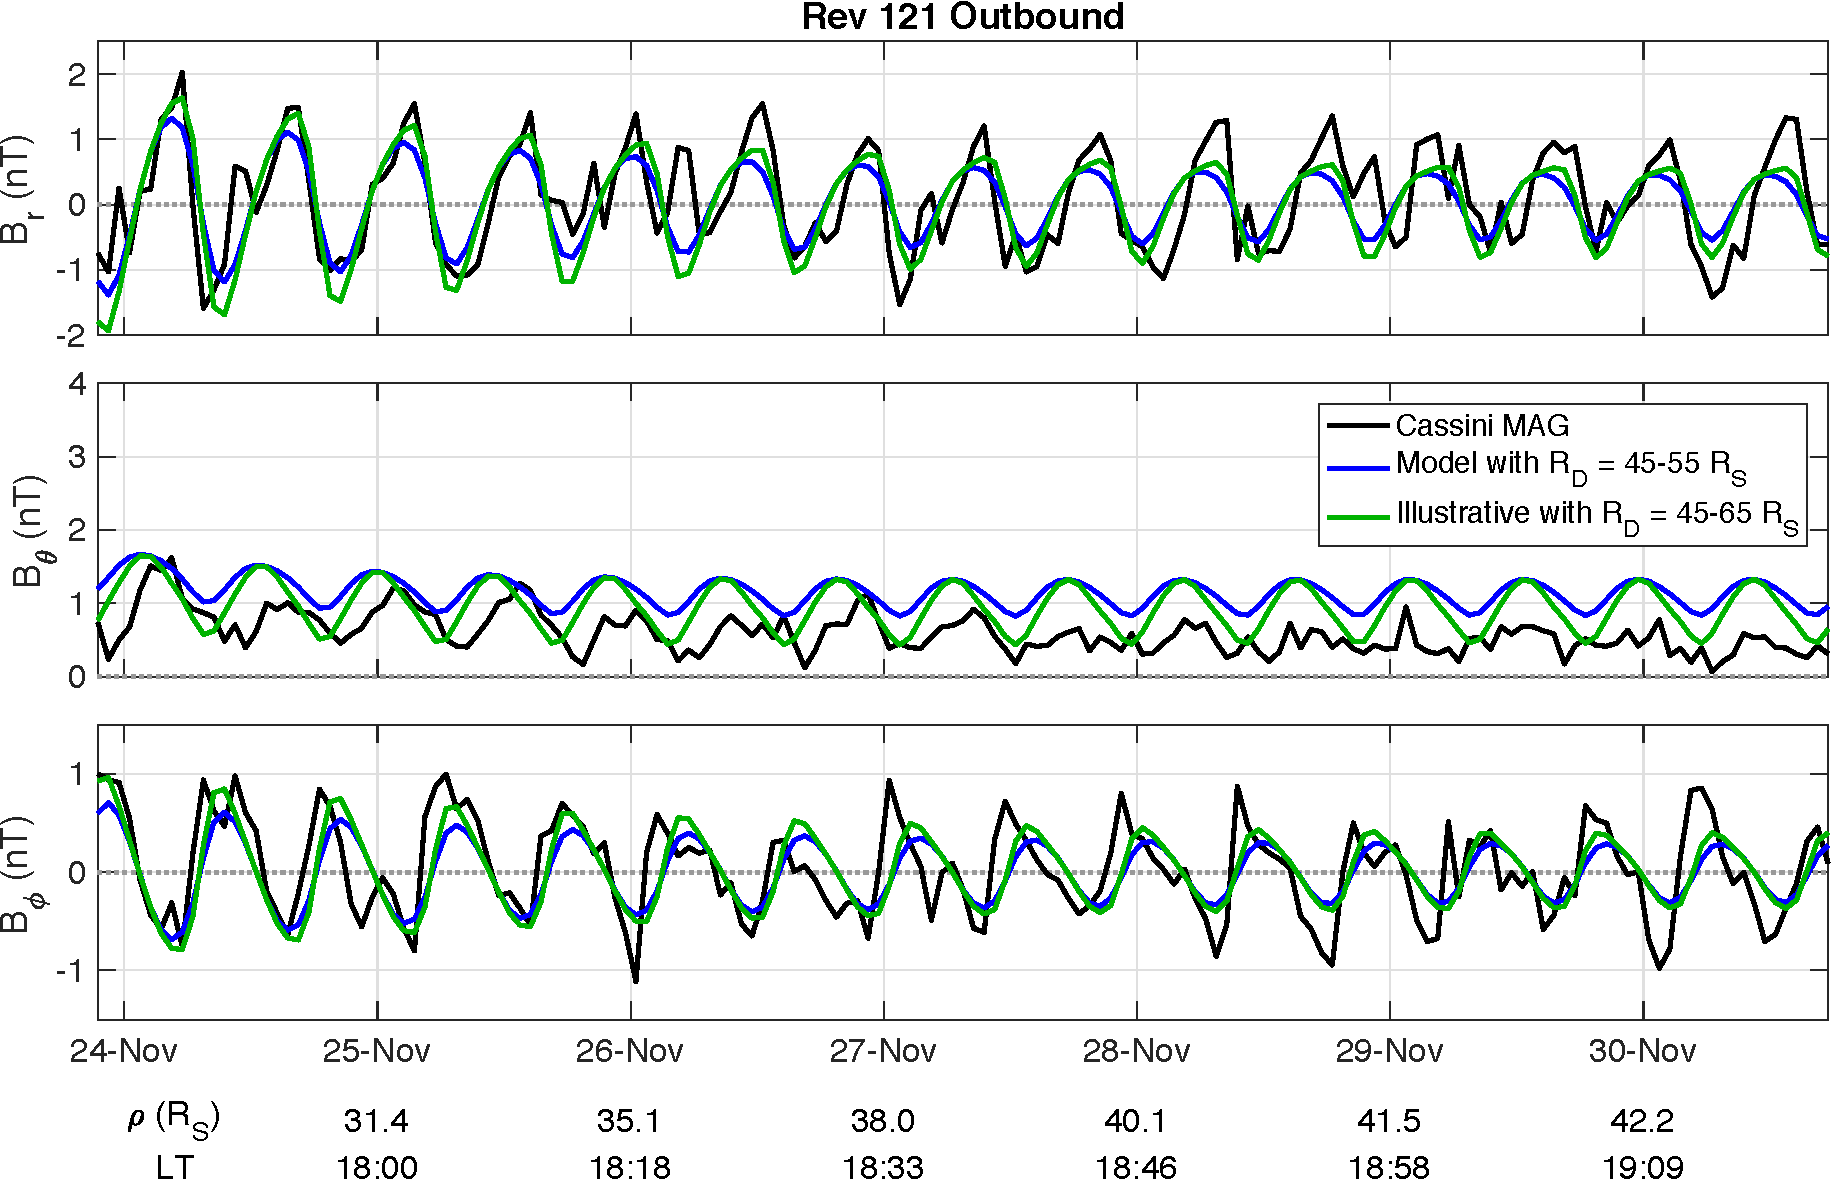
\includegraphics[width=0.8\textwidth]{equinox/rev121outdiffMDs.pdf}
\caption[\textit{Cassini} MAG data, FO and F{\&}B model predictions for Rev 121 Outbound, with modified F{\&}B model parameters.]{Similar to Figure~\ref{equinox:fig:rev120in}, for \textbf{Rev 121 Outbound}. MAG data is shown in black, in blue is a reproduction of the best-fit flapping and breathing model for Rev 121 Outbound from Figure~\ref{equinox:fig:rev121out}, and in green is flapping and breathing model using same parameters, but a larger range of magnetodisc model radii as shown by the legend.}
\label{equinox:fig:rev121outdiffMDs}
\end{figure}

The discrepancy between model and data for the average values of $B_{\theta}$ may also be due to our parameterisation of the hot plasma content $K_\mathrm{H}$ in the magnetodisc model. The predicted values of $B_{\theta}$ are sensitive to our choice of $K_\mathrm{H}$, with, in general, higher hot plasma content producing higher magnetic field strengths in the outer magnetosphere, and more disc-like magnetic field structures, due to global pressure balance \citep[see][]{achilleos2010b,sorba2017}. This type of structure is also, in general, associated with a more extreme variation in the magnitude of the radial component of the magnetic field above and below the equatorial plane. Our choice of $K_\mathrm{H}$ could therefore affect our fitting of the tilt angle $\theta_\mathrm{T}$, which controls the amplitude of the oscillations in $B_r$, particularly for the FO model. As discussed in Section~\ref{equinox:sec:modelparamzation} we use a value of $K_\mathrm{H}$ appropriate for the entire data set studied here, and in line with previous results of global average values. However the appropriate $K_\mathrm{H}$ for the region local to \textit{Cassini} may well vary from pass to pass depending on local conditions, and we can see from Figure~\ref{equinox:fig:hotpressuremodel} that the hot plasma pressure varies significantly within our interval of study. This explanation would also be consistent with the observation that our models underestimate the average $B_{\theta}$ in some passes and overestimate in others, rather than systematically overestimating or underestimating across all passes. This could also potentially explain why we find a range of best-fit $\theta_\mathrm{T}$ values that, while consistent with previous results, show significant spread from pass to pass. However, we find that the observed hot plasma pressure varies significantly from a given model profile shown in Figure~\ref{equinox:fig:hotpressuremodel}, even within one single Rev as separated in this study. This comparison implies that even using different values of $K_\mathrm{H}$ from pass to pass could not capture the hot plasma variations in their entirety. Similar variability has been observed and discussed in studies such as \citet{sergis2007} and \citet{kellett2010}.

Additionally, the magnetodisc model assumption of a single ion mass along each field line, previously mentioned in Section~\ref{equinox:sec:plasmamodel}, means that the model does not account for fine variation in magnetodisc structure caused by a concentration of heavier ions near the current sheet, which could lead to a putatively thinner current sheet at large radial distance \citep{nemeth2011}. This effect would generally be associated with an even lower value of $B_{\theta}$ than we predict herein, particularly in the outer magnetosphere. Plasma sheet thickness can also vary unsystematically on timescales as short as a single \textit{Cassini orbit}, potentially due to a combination of internal and external influences, as shown by \citet{sergis2011}.

Saturn's current sheet thickness also varies with local time, which is not directly accounted for by our model, as discussed in Section~\ref{equinox:sec:simulatingbreathing}. The range in local time for each \textit{Cassini} pass studied here is only $\sim2-3.5$ hours, and so within a given pass any variation in sheet thickness associated with local time is likely to be less significant than the variation due to the magnetodisc breathing behaviour. For the entire data set studied here, the local time range is approximately 15:45-22:45, with 80\% of the data in the range 18:00-21:00, which could introduce variations between passes in how well our model characterises the data; however, observation of Figures~\ref{equinox:fig:rev120in}-\ref{equinox:fig:rev122out} does not reveal a significant relationship between model-data discrepancies and the local time range of the given pass.

Looking at each pass individually, the best fit parameters for the F{\&}B model are in general consistent with those of the FO model, suggesting that the FO model is an appropriate approximation at least for modelling the $B_{r}$ and $B_{\phi}$ components of the magnetic field. Specifically, for all but Rev 122 Inbound, the fitted values of $\lambda_0$ agree for each model within uncertainties, and the fitted values for $\theta_\mathrm{T}$ are lower for the F{\&}B model than the FO model. This can be understood as $\theta_\mathrm{T}$ controls the amplitude of the oscillations in the magnetic field associated with the flapping, and so introduction of the breathing behaviour allows some of this amplitude to be `accounted for' by the breathing perturbation. It is perhaps not surprising that Rev 122 Inbound is the exception to this observed behaviour, as Figure~\ref{equinox:fig:rev122in} shows there is very little observed periodic oscillation in $B_{\theta}$ during this pass, meaning the F{\&}B model is not well constrained. In addition, on this pass a transient negative $B_{\theta}$ signature can be seen around 7 December, which is associated with a region of higher density, lower energy plasma in the CAPS-ELS data. This may be a signature of a small-scale `ballooning' instability of the plasma sheet, resulting in a northward turning of the magnetic field in the centre of a localised plasma `bubble', similar to events observed at Jupiter by {\citet{kivelson2005}. This event appears to perhaps be immediately preceded by an episode of current sheet thinning, as revealed by larger amplitude oscillations in the radial component of the field compared to both the model predictions, shown in Figure~\ref{equinox:fig:rev122in}.} This suggests a very dynamic plasma sheet in this region, and perhaps explains why our models do not reproduce the data for Rev 122 Inbound in particular. It is interesting to note that immediately after the event $B_\theta$ appears to peak when $B_r$ is close to 0, perhaps suggesting a return to flapping-only-like behaviour after this event. Similar transient negative $B_\theta$ signatures can be seen in Rev 121 Inbound around 17{\--}18 November, (Figure~\ref{equinox:fig:rev121in}), and again are accompanied by more variable, aperiodic magnetic field signatures that cannot be characterised by our models.

In general the best fit values of $\lambda_\mathrm{B}$ show large variation pass to pass, and have larger uncertainties as they are only significantly constrained by the behaviour of the $B_{\theta}$ component. As described in Section~\ref{equinox:sec:simulatingbreathing}, this parameter $\lambda_\mathrm{B}$ determines the approximate longitude at which the maximum disc model radius is used at $\rho = \rho_0$, which in our model is the same as the region with the thinnest, most radially distended current sheet. Looking at Figure~\ref{equinox:fig:CowleyTDdiagrams}, we can see that for a magnetosphere system dominated by the southern perturbation, we would expect values of $\lambda_\mathrm{B}$ and $\lambda_\mathrm{0}$ to be similar, as the maximum vertical displacement of the current sheet and the maximum radial distortion of the current sheet are at the same longitude in panel (d). While we do observe this for one pass, there is considerable spread among the other passes. Meanwhile for a system dominated by the northern perturbation, from Figure~\ref{equinox:fig:CowleyTDdiagrams} we would expect to observe $\lambda_\mathrm{B}$ and $\lambda_\mathrm{0}$ approximately $\SI{180}{\degree}$ apart, as in panel (b) the longitude of the maximum vertical displacement of the current sheet is diametrically opposite to the longitude where the current sheet is most radially distended. However we find that our measured values of $\lambda_\mathrm{B}$ are not, in general, compatible with this picture either. This suggests that the northern and southern magnetic perturbations are of similar amplitude during this time period, which indeed was observed by \citet{andrews2012}, and thus are both controlling the dynamics of the magnetodisc to varying degrees. Indeed, as described in the recent study by \citet{cowley2017b}, the true behaviour of the magnetodisc is more complicated than this simplified interpretation of diagrams of Figure~\ref{equinox:fig:CowleyTDdiagrams}, with the current sheet thickness modulated differently in the northern and southern hemispheres depending on the phase difference between the two rotating magnetic perturbations. In this study we only explicitly allow one thickness modulation, at the phase $\lambda = \lambda_\mathrm{B}$, and so even our F{\&}B model cannot fully resolve this behaviour. In a study by \citep{provan2012}, the authors observe that the modulation in current sheet thickness is most extreme, by a factor of ${\sim}2$, when the northern and southern perturbations are in antiphase. In this study we use a fixed current sheet thickness modulation, fully controlled by our chosen range in disc model radius $R_\mathrm{D}$, and so cannot resolve at what phase differences we observe the greatest variation in current sheet thickness. However we intend to address this in a future study either by allowing the range of $R_\mathrm{D}$ to vary as a free parameter, or similar alternative approaches, discussed below in Section~\ref{equinox:sec:constDp}.

Another complicating factor for our best fit parameters is our choice of the delay parameter $D = \Omega_S/v_\mathrm{w} = \SI{3}{\degree/R_S}$. This predominantly influences the phasing rather than the amplitude of the model oscillations; for larger values of $D$, the spiral pattern shown in Figure~\ref{equinox:fig:cssurfacemodel} becomes more tightly wound, and so the period of the oscillations generally becomes shorter with increasing radial distance. This particularly affects our fitting of the parameter $\lambda_0$, as this parameter also influences the model phasing by controlling the phase of the maximum flapping perturbation. As previously discussed, the data sets studied here are restricted in local time to the dusk sector, with the majority of observations in the local time sector 18:00{\--}21:00, and no single pass spanning more than 3.5 hours of local time. Therefore the aforementioned variation in magnetospheric wavespeeds reported in \citet{andrews2010} is unlikely to have a large influence. However the possible variation in wavespeeds with radial distance and local conditions, as discussed in Section~\ref{equinox:sec:cssmodel}, may be a source of discrepancy between our models and results. 

As a preliminary investigation, we re-fit the F{\&}B model to the Rev 120 Inbound pass data using a greater value for the delay parameter $D = \SI{5}{\degree/R_S}$, chosen as roughly the upper limit of an expected appropriate value for $D$ as discussed in Section~\ref{equinox:sec:cssmodel}. We found that the resulting best fit parameters were not significantly altered for this fit, with $\theta_\mathrm{T}$ and $\lambda_\mathrm{B}$ both equivalent to the values presented in Table~\ref{equinox:table:fitparams} within uncertainties, and the value of $\lambda_0$ differing by around 9\%, broadly as expected as this parameter is most strongly affected by the phasing controlled by the specific value of $D$. We also found that the RMS residual between model and data was around 6\% greater for this model than for our original model with $D = \SI{3}{\degree/R_S}$, suggesting this original lower value of $D$ is appropriate for the best fit in this case.

In addition, with the F{\&}B model we attempt to characterise both the rotational flapping perturbation and the compressional breathing perturbation. Intuitively, the delay in the flapping perturbation could be considered to be controlled by the local Alfv\'{e}n speed of the magnetospheric plasma, with information traveling from the magnetic poles to the current sheet along magnetic field lines, because this is a rotational perturbation causing a displacement of the current sheet. In contrast the breathing perturbation could be considered to be controlled by the plasma magnetosonic speed, with information traveling radially outwards in the equatorial region towards the outer magnetosphere, perpendicular to magnetic field lines, because this is a compressional perturbation. This means that it may be more appropriate to use different delay parameters for the two different perturbations. This more complicated picture for local phase determination is beyond the scope of this current work, but would be rewarding to investigate in future.

As discussed in Section~\ref{equinox:sec:method}, in this study we use a longitude system based on the southern magnetic perturbation from \citet{andrews2012}, as the amplitude of this perturbation was greater than or similar to the northern perturbation in the equinox period being studied here. In addition, this allowed for a direct comparison with the results of \citet{arridge2011}. However there is no fundamental physical reason why we could not have used a system based on the northern magnetic perturbation instead. While the amplitude of the oscillations in the magnetic field are unlikely to be affected by such a change, the phasing of the oscillations would be, as the rotation period associated with the northern perturbation is shorter than for the southern. However, as discussed in Section~\ref{equinox:sec:intro}, this difference became smaller in the period after Saturn equinox, to around $\SI{0.1}{\hour}$ for the time period being studied here. A preliminary investigation with the Rev 120 Inbound pass showed that the best fit parameters were not significantly altered when using the northern perturbation to organise the oscillations, with the best fit $\theta_\mathrm{T}$ equivalent to the value presented in Table~\ref{equinox:table:fitparams} within the measured uncertainty, and the difference between the parameters $\lambda_0$ and $\lambda_\mathrm{B}$ for the F{\&}B model also the same within uncertainties to the results presented here. Note that when using the northern perturbation we would not expect the actual absolute values for $\lambda_0$ and $\lambda_\mathrm{B}$ to be equal to those presented here, as they would be measured relative to that new longitude system. Therefore only the difference between the two parameters is comparable, and even this value is somewhat influenced by using the new longitude system due to the aforementioned difference in rotation period for the northern perturbation. Whilst by no means a comprehensive analysis, this result is reassuring and suggests that our main conclusions would not be significantly altered if we were to use the northern perturbation as a longitude system instead.

\subsection{Consideration of Equilibrium and Constant Solar Wind Dynamic Pressure}\label{equinox:sec:constDp}
If the compressional breathing perturbation, and consequent movement of the magnetopause boundary, is triggered by an internal source within the magnetosphere, then the appropriate family of magnetodisc models used to simulate this behaviour should ideally represent an equivalent system under constant solar wind dynamic pressure. However in this study, the magnetodisc models contain no source of internal pressure perturbation, but are calculated assuming magnetostatic equilibrium for different disc radii, and, therefore, different upstream solar wind dynamic pressure. This is done to try and reproduce the reconfiguration in magnetic field associated with the breathing dynamics. In the study presented in Chapter~\ref{chap:compress}, we estimated the incident solar wind dynamic pressure $D_\mathrm{P}$ corresponding to a given magnetodisc model by simply summing the magnetic and plasma pressure components just inside the magnetopause boundary at the nose of the magnetodisc, thus assuming pressure balance across the magnetopause at the subsolar point. We use the same approach here for our family of magnetodisc models used to simulate the breathing behaviour. However unlike in Chapter~\ref{chap:compress}, our analysis is not restricted to the nose of the magnetodisc, where the solar wind is normal to the magnetopause surface, and we therefore must account for the angle $\psi$ between the incident solar wind and the magnetopause surface normal. We discussed in Section~\ref{intro:sec:pbalance} how the full form of pressure balance across the magnetopause surface is be given by 
\begin{equation*}\label{equinox:eq:pbalance}
\frac{B_\mathrm{MS}^2}{2\mu_0} + P_\mathrm{MS} = [k\cos^2(\psi) + \frac{k_\mathrm{B}T_\mathrm{SW}}{1.16m_\mathrm{p}u_\mathrm{SW}^2}\sin^2(\psi)] D_\mathrm{P} \tag{\ref{intro:eq:pbalance2} revisited}
\end{equation*}
from \citet{kanani2010}, based on the formulation by \citet{petrinec1997}. The terms on the left represent the magnetospheric magnetic and plasma pressures just inside the magnetopause boundary, and the terms on the right (the coefficients of solar wind dynamic pressure $D_\mathrm{P}$) represent the component of solar wind dynamic pressure incident on the magnetopause surface, and a smaller component associated with the solar wind's thermal pressure (see \citet{kanani2010}). $k = 0.881$ is a factor to account for the diversion of flow around the magnetosphere obstacle, and $T_\mathrm{SW}$ and $u_\mathrm{SW}$ are the temperature and speed of the solar wind. It was shown by \citet{kanani2010} that the estimated dynamic pressure is insensitive to the choice of $T_\mathrm{SW}$ and $u_\mathrm{SW}$ as for any reasonable choice, this term is significantly smaller than the first $D_\mathrm{P}$ term for the full range of $\psi$ over which the magnetopause surface model is valid. Nevertheless we use the full form of equation~(\ref{equinox:eq:pbalance}) here with $k_\mathrm{B}T_\mathrm{SW} = \SI{100}{eV}$ and $u_\mathrm{SW} = \SI{460}{\km\per\second}$ following \citet{pilkington2015}. At the magnetopause nose $\psi = \SI{0}{\degree}$ as the magnetopause surface is perpendicular to the incident solar wind, and as you move anti-sunward along the magnetopause surface this value increases, and so the second $D_\mathrm{P}$ term becomes comparatively greater. At the dusk flank, at the location of the most anti-sunward magnetopause crossing in our data set, shown in Figure~\ref{equinox:fig:crossingssurface}, the \citet{pilkington2015} surface models shown there have $\psi \approx \SI{67}{\degree}$. This gives a coefficient of $D_\mathrm{P}$ in equation~\ref{equinox:eq:pbalance} of $0.135 + 0.033 \approx 0.17$. If we take our magnetodisc model family to be representative of the magnetosphere in that region, we can then estimate the incident solar wind dynamic pressure $D_\mathrm{P}$ by the sum of the internal magnetic and plasma pressures just inside the model magnetopause boundary, divided by this value 0.17, following equation~\ref{equinox:eq:pbalance}.

Table~\ref{equinox:table:EdgePs} shows this calculation for the family of five magnetodisc models that were used to simulate the breathing behaviour in this study. We can see that the total pressure at the equator just inside the magnetopause boundary ($P_\mathrm{EDGE}$), and the corresponding estimate of $D_\mathrm{P}$, is not constant across all models, but is lowest for the largest magnetodisc model and varies by around 60\%. Hence, as we indicated earlier, this family of models does not represent a system under constant solar wind dynamic pressure.

For a more physically realistic model, we would ideally be able to simulate the breathing behaviour of the current sheet without the need to modify the implied external solar wind dynamic pressure. One potential alternative approach, which would satisfy this particular condition, is as follows. A single magnetodisc model could be used at all longitudes, with a given disc radius $R_\mathrm{D}$, as for the flapping only model. The breathing behaviour could then be simulated by varying the cylindrical radial distance $\rho_\mu$ at which magnetic field values are extracted from the magnetodisc model (see equation~\ref{equinox:eq:coordinatetransform} and discussion). This could be varied harmonically with longitude broadly as $R_\mathrm{D}$ is in our current approach, such that the local magnetodisc structure is effectively displaced inwards or outwards with respect to the spacecraft location, depending on the spacecraft longitude, while the effective solar wind dynamic pressure corresponding to that underlying magnetodisc model remains constant. While beyond the scope of the current study, this approach may provide an interesting comparison to the work presented here in terms of the amplitude and shape of the magnetic field oscillations, and may be investigated in more detail in future. The potential drawback of this approach is that it would not reveal explicitly how a periodic thickening and thinning of the current sheet affects the magnetic field oscillation signatures, but more how the global magnetodisc magnetic field structure varies with radial distance. While it satisfies the condition that the incident solar wind pressure is not modulated, it is a somewhat artificial method of introducing the breathing behaviour and is thus a low-order approximation of the true behaviour of the magnetodisc. Alternatively, a longitude-dependent scaling factor representing sheet thickness could be used to multiply the model coordinate $z_\mu$ (see equation~\ref{equinox:eq:coordinatetransform}. The longitude dependence could be controlled by a free parameter (much as $\lambda_\mathrm{B}$ is used in this study), but we could also potentially fit for the value of the scale factor; in this way we could investigate by how much the current sheet thickness varies for different phase differences between the Northern and Southern magnetic perturbations, and thus compare results more directly with the observations of \citep{provan2012} and \citep{cowley2017b}.
\begin{table}
\caption[Model radii and solar wind dynamic pressure estimates for breathing magnetodisc models.]{Table showing the 5 different magnetodisc models used in this study to simulate the breathing behaviour, their disc radii $R_\mathrm{D}$, the total magnetic and plasma pressure at the equator just inside the magnetopause boundary $P_\mathrm{EDGE}$, and the corresponding estimate of solar wind dynamic pressure $D_\mathrm{P}$ using equation~\ref{equinox:eq:pbalance}.}
\label{equinox:table:EdgePs}
\centering
\begin{tabular}{c c c}
\hline
$R_\mathrm{D}~(\si{R_S})$ & $P_\mathrm{EDGE}~(\si{nPa})$  & Approx $D_\mathrm{P}~(\si{nPa})$\\
\hline
45 & 0.0027 & 0.016 \\
47.5 & 0.0023 & 0.014\\
50 & 0.0020 & 0.012 \\
52.5 & 0.0018 & 0.011 \\
55 & 0.0016 & 0.010 \\
\hline
\end{tabular}
\end{table}

\section{Summary and Conclusions}\label{equinox:sec:conclusions}
In the study presented in this chapter, we have investigated the periodic dynamical behaviour of Saturn's equatorial current sheet during the period following Saturn equinox in late 2009, using data from \textit{Cassini's} magnetometer instrument. We have attempted to model both the periodic vertical displacement of the current sheet above and below the rotational equator (`flapping' behaviour) and the periodic thickening and thinning of the equatorial current sheet, and corresponding change in magnetic field structure from more dipolar to more disc-like (`breathing' behaviour). Both of these behaviours are thought to be controlled by the dual rotating magnetic perturbations that have been observed in Saturn's northern and southern hemispheres.

To do this modelling we have used a local, force-balance magnetic field and plasma model of Saturn's magnetodisc from \citet{achilleos2010a} (the UCL/AGA model), and geometrically anchored it to a global, geometric model of current sheet location from \citet{arridge2011}. The flapping behaviour was simulated by the periodic displacement of the model current sheet location, and the breathing behaviour was simulated by varying the magnetodisc model disc radius, and thus the magnetic field structure, with azimuth around the planet.

We found that, for those passes that show clear periodic oscillations in the magnetic field, our model characterises well both the amplitude and phase of the oscillations. In particular, the $B_\theta$ (meridional) component of the magnetic field is in general better characterised when the breathing behaviour is included, as it can better replicate both the amplitude and the dominant variation once per rotation period, rather than twice as with the flapping only model. These observations therefore support the picture described in Section~\ref{equinox:sec:intro} and previously observed by studies described therein, that the dual rotating magnetic perturbations in Saturn's magnetosphere cause a periodic modulation in the current sheet thickness, as well as in location above or below the rotational equator. In particular, we find that the \citet{arridge2011} tilted, rippled current sheet model with a value of delay parameter $D = \SI{3}{\degree/R_S}$ can accurately characterise the periodic flapping behaviour of the magnetodisc, with observed tilt angles $\theta_\mathrm{T}$ in the range $4-\SI{18}{\degree}$ for the trajectories studied here, in line with previous studies discussed in Section~\ref{equinox:sec:intro}. We also find values of $\lambda_0$ that, when using the Southern magnetic perturbation from \citet{andrews2012}, are broadly consistent with the results of \citet{arridge2011}. For the breathing parameter introduced in this study, $\lambda_\mathrm{B}$, we find significant variation between \textit{Cassini }passes, suggesting that this behaviour varies significantly on this timescale relative to the prime meridian of the flapping perturbation, likely due to the changing strengths and phase differences between the Northern and Southern magnetic perturbations. However we have shown that by harmonically varying the model disc radius by $\SI{10}{R_S}$, from $45-\SI{55}{R_S}$, we can semi-quantitatively reproduce the oscillations in the magnetic field components associated with a periodic perturbation in current sheet thickness, as described in previous studies discussed in Section~\ref{equinox:sec:intro}. This suggests that the variation in current sheet thickness between these different-sized magnetodisc models, shown in Figure~\ref{equinox:fig:MDALLcsthickness}, is broadly representative of the magnetodisc behaviour for the time interval studied.

For some passes the observed magnetic field is very variable on short timescales, perhaps due to local transient events in Saturn's plasma sheet, and our model is not capable of capturing this dynamical behaviour. In addition, one main drawback of our model is that it does not explicitly take into account the phase difference between the northern and southern rotating magnetic perturbations, instead using the phase of the southern magnetic perturbation in particular to organise the magnetic field data. This limits the the physical insights we can draw from our observations, and we hope to develop this aspect of the model further in a future study. However, the relative strength of the current approach is that the model can capture the observed behaviour of the magnetic field rather well for much of the time interval studied, with relatively few fitted or fixed parameters.

The treatment of the delay parameter $D$, discussed in Section~\ref{equinox:sec:method}, is another area where we hope to develop this model further, perhaps using other data sets to further constrain the appropriate choice of $D$, and in particular how it may vary with radial distance and local time. This may improve the agreement between the model and the data particularly in the phasing of the oscillations. A more realistic representation may also elucidate the physics of how the rotating magnetic perturbations, which are thought to originate from vortices in Saturn's upper atmosphere and ionosphere \citep[e.g.][]{jiaandkivelson2012}, actually control the dynamics much further out in Saturn's outer magnetosphere. As discussed in Section~\ref{equinox:sec:results}, there is also scope to more realistically simulate the current sheet breathing behaviour, by using a harmonic variation in the radial distance at which the magnetodisc model is sampled, or modifying the vertical distance at which the model is sampled by a given scale factor, such that our model represents a system under constant solar wind dynamic pressure. These approaches may be pursued in more depth in a future study.

This work contributes to our current understanding of the periodic perturbations observed in Saturn's outer magnetosphere, combining recent knowledge acquired from both modelling approaches and long-term \textit{Cassini} measurements. In particular it provides a way of understanding and parameterising these perturbations in terms of a periodic vertical displacement and thickness modulation of the current sheet, controlled in a complex and variable way by the proposed hemispheric rotating perturbations in the magnetic field.

In this chapter we investigated the structure of the current sheet specifically in the local time region 15:45-22:45, with 80\% of the data in the range 18:00-21:00. Therefore  we did not  explicitly account for any local time variations in the current sheet thickness in our investigation. However  in conducting this study it  became apparent that an understanding of how the current sheet and overall magnetodisc structure varies at different local time sectors would  be useful in future studies looking at this phenomenon. In Chapter~\ref{chap:LTsectors}, we investigate this in detail using the UCL/AGA model once again, in combination with recently published observations of the hot plasma population from \textit{Cassini} MIMI data.
\chapter{Local Time Variation in Large-Scale Structure of Saturn's Magnetosphere}
\label{chap:LTsectors}
Throughout this thesis, we have shown how the large-scale structure of Saturn's magnetosphere is determined by internal and external factors, including the rapid planetary rotation rate, significant internal hot and cold plasma sources, and varying solar wind pressure. However it is still not fully understood which factors dominantly influence the configuration of the magnetosphere, and in particular how this relationship varies with local time. In this chapter, we explore this in detail using the UCL/AGA model Saturn's magnetodisc to describe the magnetosphere at different local time sectors. For model inputs, we use recent observational results which suggest a significant local time asymmetry in the pressure of the hot plasma population, and magnetopause location. We make calculations under different solar wind conditions, in order to investigate how these local time asymmetries influence magnetospheric structure for different system sizes. We find significant day/night asymmetries in the model magnetic field, consistent with recent empirical studies based on \textit{Cassini} magnetometer observations. We also find dawn-dusk asymmetries in equatorial current sheet thickness, with the varying hot plasma content and magnetodisc radius having comparable influence on overall structure, depending on external conditions. We also find significant variations in magnetic mapping between the ionosphere and equatorial disc, and ring current intensity, with substantial enhancements in the night and dusk sectors. These results have consequences for interpreting many magnetospheric phenomena that vary with local time, such as reconnection events and auroral observations. \\
\\
The contents of this chapter are based on the study: \\
\\
\bibentry{sorba2019}. 

\section{Introduction to this Study}\label{LTsectors:sec:intro}
In recent years, a more global understanding of Saturn's magnetosphere has become possible largely thanks to the extensive temporal, spatial and seasonal coverage of the \textit{Cassini} space mission. \textit{Cassini} toured the Saturnian magnetosphere from 2004 to 2017, as described in detail in Chapter~\ref{chap:cassini}. In particular, there is now an opportunity to investigate in more detail how the large-scale structure of Saturn's magnetosphere varies with \textit{local time}, and which factors control this behaviour. This information is important for interpreting a range of phenomena at Saturn; for example the likelihood of reconnection events in different regions of the magnetosphere \citep{delamere2015}, which is related to how current sheet thickness varies with local time \citep{kellett2011}. Understanding more about the structure of the current sheet is also important for studies of the observed periodicities at Saturn's magnetosphere, which investigate the periodic modulation of the position and thickness of the equatorial current sheet, as in the study we presented in Chapter~\ref{chap:equinox}. More generally, a picture of the global magnetic field structure at different local times can be useful for understanding how different regions of the magnetosphere magnetically map to the polar ionosphere in different local time sectors, for example when interpreting observations of Saturn's aurora. The recently published empirical magnetic field model by \citet{carbary2018} suggests significant day-night asymmetry in equatorial-ionospheric magnetic mapping profiles, and local time asymmetries in the location of Saturn's aurora have been observed in studies such as \citet{badman2006,badman2011}.

A recent empirical study of magnetopause crossings by \citet{pilkington2015b} showed evidence of a dawn-dusk asymmetry in the typical location of the magnetopause boundary, with in general a larger magnetopause radius on the dawn flank. In addition, a survey of magnetospheric plasma populations from \citet{sergis2017} showed significant local time asymmetry in the hot plasma population, with enhanced pressures in the dusk and midnight local time sectors compared to dawn and noon. These factors will therefore influence the magnetic and plasma configuration of the magnetosphere differently at different local times. It was shown by \citet{achilleos2010b} that variations in the hot plasma pressure have a significant impact on the magnetospheric magnetic field configuration. They found that a globally elevated hot plasma pressure causes a more disc-like magnetic field structure, due to the enhancement of the equatorial ring current, and that this also influences the magnetic mapping between the equatorial disc and the ionosphere. We presented results consistent with this in Chapter~\ref{chap:compress}. We have also previously discussed in this thesis how our modelling results suggest that more expanded systems, with larger magnetopause radii, typically have a more disc-like magnetic field structure, due to overall force balance, and that this is consistent with other studies such as \citet{bunce2008} and \citet{arridge2008}. In particular \citet{arridge2008} found that in the noon sector, Saturn's magnetosphere only showed a significant divergence from a dipolar field structure for a magnetopause radius greater than ${\sim}\SI{23}{R_S}$, but that the magnetodisc structure is consistently observed on the dawn/dusk flanks and nightside.

In this work we investigate the relative importance of the hot plasma pressure and magnetopause radius asymmetries in controlling magnetospheric structure at different local time sectors using a modelling approach, to complement observational studies. We use the previously described UCL/AGA model, adapted to describe the typical, equilibrium conditions of Saturn's magnetosphere at four different local time sectors; noon (09:00-15:00), dawn (03:00-09:00), dusk (15:00-21:00) and night (21:00-03:00). We use equatorial profiles of the hot plasma pressure from \citet{sergis2017} for the different local time sectors as boundary condition inputs to the magnetodisc model, and determine appropriate magnetopause radius values to use for each sector based on the magnetopause surface model of \citet{pilkington2015b}. Our method of constructing these models is described in Section~\ref{LTsectors:sec:method}. In Section~\ref{LTsectors:sec:results} we present the results of these calculations, and highlight interesting comparisons in the magnetic field structure, azimuthal current density and magnetic mappings for the different local time sectors. Section~\ref{LTsectors:sec:conclusions} provides a brief summary of the main conclusions of this work.

\section{Method}\label{LTsectors:sec:method}
We use the UCL/AGA model first set out in \citet{achilleos2010a, achilleos2010b} and described in Section~\ref{intro:sec:forcebalancemodel}, with modifications to boundary conditions as described in Chapter~\ref{chap:equinox}, and additional modifications described in this section. As a reminder, this 2-D, axisymmetric force-balance model assumes the magnetospheric plasma comprises a cold population confined towards the rotational equatorial plane due to the centrifugal force exerted on it, and a hot population with associated plasma pressure $P_\mathrm{H}$ constant along magnetic field lines. The model calculates Saturn's magnetic field and plasma structure by iteratively solving a partial differential equation for the magnetic potential $\alpha$, and we consider the model to have converged when the relative difference between successive iterations falls below a given tolerance, as described in Section~\ref{intro:sec:forcebalancemodel}. In this study we found that, for nightside models with especially large disc radii, it was necessary to weight the previous solution up to nine times more heavily than the present solution in order to achieve convergence, corresponding to $\gamma=0.1$ in equation~(\ref{intro:eq:convergence}). This is a consequence of extending our use of this model to more extreme regimes.

As we have seen in this thesis, the UCL/AGA model was originally used to represent typical dayside conditions at Saturn, and so we made various modifications described herein, which are necessary to appropriately represent different local time sectors.

\subsection{Hot Plasma Parameterisation for Different Local Time Sectors}\label{LTsectors:sec:hotP}
\begin{table}
\caption[Coefficients of polynomial fits to the hot plasma pressure profiles from \citet{sergis2017}.]{Coefficients of fourth order polynomial fits to the logarithm of each of the hot pressure profiles shown in Figure~\ref{LTsectors:fig:hotPpolys}, as described in the main text. } \label{LTsectors:tab:hotPpolys}
\centering
\begin{tabular}{c |  c c c c}
%\hhline{-----}
\hline
Coefficient		& Noon						& Dawn			& Dusk				& Night   	\\
%\hhline{-----}
\hline
$a_0$ 				&	-5.47						& -1.96 					&	-1.36					&	-6.86	 \\
$a_1$				&	1.10							& -0.149					&	-0.311					&	2.07	\\
$a_2$				&	-0.114						& 0.0686					&	0.109					&	-0.258 \\
$a_3$ 				&	0.00514					& -0.00652				&	-0.0104				&	0.0137 \\
$a_4$ 				&	\num{-8.47e-5} 		& \num{1.83e-4} 	&	\num{2.99e-4}	& \num{-2.71e-4}	\\
\hline
% \multicolumn{2}{l}{$^{a}$Footnote text here.}
\end{tabular}
\end{table}
\begin{figure}
\centering
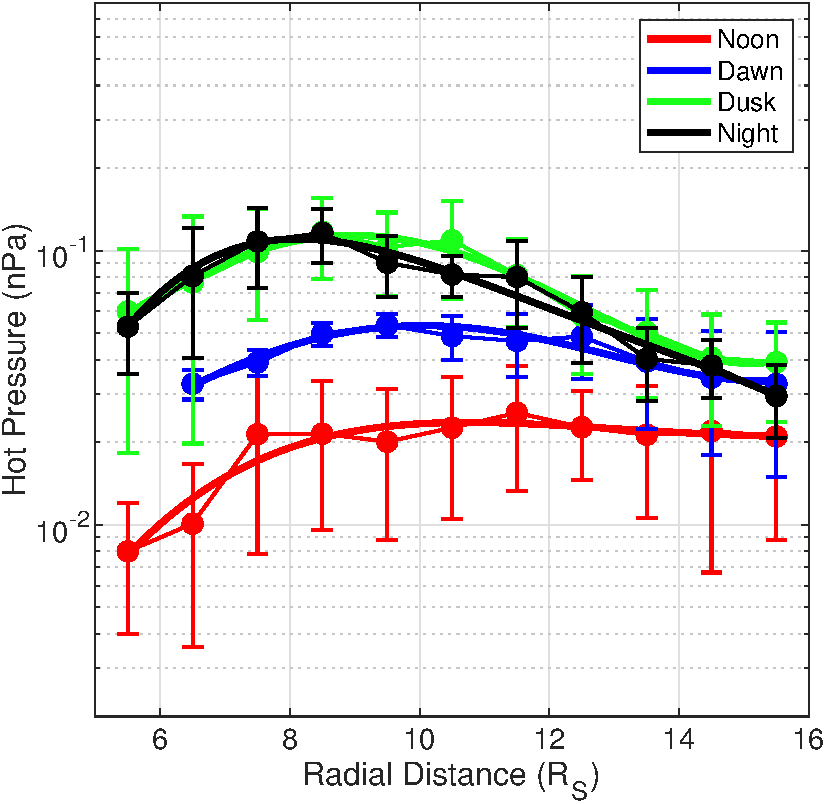
\includegraphics[width=0.6\textwidth]{LTsectors/hotPpolys.pdf}
\caption[Equatorial radial profiles of hot plasma pressure for different local time sectors from \citet{sergis2017}, with polynomial fits.]{Equatorial radial profiles of hot plasma pressure for different local time sectors, as shown by the colour. Solid circles and error bars are means and standard errors for binned data from \citet{sergis2017}, and solid lines are 4th order polynomial fits to the logarithms of the data points, as described in the main text.}
\label{LTsectors:fig:hotPpolys}
\end{figure}

The global hot plasma pressure is an important boundary condition for this model, as this strongly influences the resulting magnetic field structure. Recently, a comprehensive study using \textit{Cassini} MIMI data \citep{sergis2017} showed that the pressure of this hot plasma population not only varies over time and distance, but also varies significantly with local time, even when averaged over a large portion of the \textit{Cassini} mission (July 2004 - December 2013). Therefore in this study, we used average equatorial profiles of hot plasma pressure between $5.5$ and $\SI{15.5}{R_S}$ presented in \citet{sergis2017} for the different local time sectors, as boundary conditions for our models. Specifically, we fit the $\SI{1}{R_S}$-width-binned data presented in \citet{sergis2017} using polynomial functions of the form 
\begin{equation} \label{LTsectors:eq:fourthorderpoly}
\log(P_\mathrm{H}) = a_0+a_1\rho + a_2\rho^2 + a_3\rho^3 + a_4\rho^4
\end{equation}
following the approach used in \citet{sergis2017}  for the total plasma population, with each point weighted by the inverse square of the provided standard error of the mean. The resulting coefficients for each sector are shown in Table~\ref{LTsectors:tab:hotPpolys}, with pressure in units of $\si{nPa}$ and radial distance in units of $\si{R_S}$. The best fit polynomials are shown in Figure~\ref{LTsectors:fig:hotPpolys}, as well as the corresponding observations from \citet{sergis2017}, with standard error of the mean of each bin shown by the error bars. This figure shows that the hot plasma pressure is significantly higher in the dusk and night sectors than the dawn and noon sectors. Here the dawn, noon, dusk and night sectors are defined by the magnetic local time intervals 03:00-09:00, 09:00-15:00, 15:00-21:00 and 21:00-03:00 respectively.

For values of $\rho$ smaller than the applicable range of the polynomials ($\SI{5.5}{R_S}$) we assumed the hot plasma pressure falls linearly to zero with $\rho$, broadly in line with observations and with the approach of \citet{achilleos2010a}. For the dawn profile we used an inner boundary of $\SI{6.5}{R_S}$ due to lack of data in the innermost bin in the \citet{sergis2017} data, which can be seen in Figure~\ref{LTsectors:fig:hotPpolys}. For values of $\rho$ above the applicable range of the polynomials ($\SI{15.5}{R_S}$), we assumed a profile where the product of the hot plasma pressure and the local flux tube volume is constant with radial distance, following previous studies such as \citet{achilleos2010a} and our study in Chapter~\ref{chap:compress}. In practice for the dawn and dusk models we used outer limits of $\SI{15.3}{R_S}$ and $\SI{15.1}{R_S}$ respectively, which are the locations of the local minima in the hot pressure polynomials, to ensure a smoother profile.

\subsection{Magnetopause Radius for Different Local Time Sectors}
\begin{table}
\caption[Details of the magnetodisc radius, shielding magnetic field value and $D_\mathrm{P}$ estimate for each local time sector model.]{Configuration details for the two families of models used to represent different local time sectors, for compressed (high solar wind dynamic pressure) and expanded (low solar wind dynamic pressure) regimes. magnetodisc radius, shielding magnetic field value and an estimate for the solar wind dynamic pressure $D_\mathrm{P}$ are shown for each model.}\label{LTsectors:tab:modelparams}
\centering
\begin{tabular}{l l c c c}
\hline
%Regime									&	LT Sector		& disc Radius ($\si{R_S}$)		& Shield $B_z$ ($\si{nT}$)		& $D_\mathrm{P}$ estimate ($\si{nPa}$)\\
Regime									&	LT Sector		& \makecell{Disc Radius \\ ($\si{R_S}$)}		& \makecell{Shield $B_z$ \\ ($\si{nT}$)}		& \makecell{$D_\mathrm{P}$ estimate \\ ($\si{nPa}$)}\\
\hline
\multirow{4}{*}{Compressed} & Noon			&	21.0										& -2.62									& 0.031 \\
												& Dawn			& 34.3										& -0.97									& 0.026 \\
												&	Dusk			&	33.2										&	-0.88									& 0.030 \\
												& Night			& 42.0										& 0.14										&	- \\
\hline
\multirow{4}{*}{Expanded}  	& Noon			& 27.0										& -1.40									& 0.012 \\
												& Dawn			& 43.8										& -0.47									&	0.015 \\
												& Dusk				& 42.3										& -0.41									& 0.016 \\
												& Night			& 54.0										& 0.13										& - \\
\hline
\end{tabular}
\end{table}

The UCL/AGA model used can also be parameterised by an effective disc radius $R_\mathrm{D}$, the equatorial radial distance of the last closed field line in the model. As discussed in Section~\ref{LTsectors:sec:intro} and throughout this thesis, variations in this quantity also significantly impact the resulting magnetic field structure in the model. It was therefore important for this work that we chose appropriate values of the disc radius $R_\mathrm{D}$ for each of the local time sectors we were describing. To do this, we appealed to the study of \citet{pilkington2015b}, who improved the earlier Saturn magnetopause surface models of \citet{pilkington2015, kanani2010, arridge2006} by in particular including a small dawn-dusk asymmetry in magnetopause radius in the model. In \citet{pilkington2015b} the authors used observations of magnetopause crossings made throughout a large portion of the \textit{Cassini} mission to constrain parameters for a \citet{shue1997} type magnetopause model, introducing an extra parameter to describe the dawn-dusk asymmetry whilst maintaining a continuous surface at the magnetopause nose. They found that on average the magnetopause boundary extends farther from the planet on the dawn side than the dusk side, by ${\sim}7\%$. 

In order to investigate how local time variation in magnetospheric structure varies with system size, we calculated two sets of models under different solar wind dynamic pressure conditions; a compressed regime with subsolar magnetopause radius fixed at $\SI{21}{R_S}$, and an expanded regime with subsolar magnetopause radius fixed at $\SI{27}{R_S}$, following the bimodal values observed in \citet{pilkington2015} and \citet{achilleos2008}. For the corresponding dawn and dusk disc radii, we calculated the magnetopause radius at the center of each local time sector (06:00 for dawn and 18:00 for dusk) using the best fit parameters given in \citet{pilkington2015} and \citet{pilkington2015b}. We used a value of the nose plasma $\beta = 3$, which is the median value for the dataset of magnetopause crossings provided in \citet{pilkington2015}, although for a fixed subsolar radius this choice of $\beta$ had very little impact on the resulting flank radii. Thus we determined the appropriate disc radii $R_\mathrm{D}$ for noon, dawn and dusk local time sectors, for both high and low solar wind pressure conditions. The resulting values are shown in Table~\ref{LTsectors:tab:modelparams}. In the absence of an accurate magnetopause model for the nightside of Saturn's magnetosphere, we used a disc radius of twice the subsolar magnetopause radius to represent an approximate nightside local time sector structure.

The solar wind dynamic pressure corresponding to a given equilibrium magnetodisc model can be estimated by assuming pressure balance across the boundary at the equator, as in Chapters~\ref{chap:compress} and \ref{chap:equinox}. Specifically we can assume
\begin{equation}\label{LTsectors:eq:pbalance}
\frac{B_\mathrm{MS}^2}{2\mu_0} + P_\mathrm{MS} = \left[k\cos^2(\psi) + \frac{k_\mathrm{B}T_\mathrm{SW}}{1.16m_\mathrm{p}u_\mathrm{SW}^2}\sin^2(\psi)\right] D_\mathrm{P} \tag{\ref{intro:eq:pbalance2} revisited}
\end{equation}
where terms on the left hand side represent the magnetospheric  magnetic and plasma pressures just inside the magnetopause boundary, and the terms on the right  represent the component of solar wind dynamic pressure incident on the magnetopause surface, and a smaller component associated with the solar wind's thermal pressure. As before, $k = 0.881$ is a factor to account for the diversion of flow around the magnetosphere obstacle \citep[see][]{spreiter1966}, $k_\mathrm{B}T_\mathrm{SW} = \SI{100}{eV}$  and $u_\mathrm{SW} = \SI{460}{\km\per\second}$ are the temperature and speed of the solar wind from \citet{pilkington2015}, and $\psi$ is the angle between the incident solar wind and the magnetopause surface normal. We used values for $B_\mathrm{MS}$ and $P_\mathrm{MS} = P_\mathrm{H} + P_\mathrm{C}$ extracted just inside the magnetopause boundary of each model, and obtained $\psi$ from the \citet{pilkington2015b} magnetopause surface model at the appropriate local time sector. The resulting estimates of $D_\mathrm{P}$ are shown in Table~\ref{LTsectors:tab:modelparams}. This approach is not appropriate for the far night-side tail, where a concept of $\psi$ is not directly applicable, and so we do not attempt to estimate $D_\mathrm{P}$ for those sector models. While the values of $D_\mathrm{P}$ do not exactly agree for all compressed or all expanded models, we can see that the two regimes provide significantly different, self-consistent estimates. The mean $D_\mathrm{P}$ estimates are $0.029\pm\SI{0.003}{nPa}$ and $0.015\pm\SI{0.002}{nPa}$ for the compressed and expanded regimes respectively, such that they broadly correspond systems under different solar wind conditions, whilst representing average internal conditions.

\subsection{Magnetodisc Model Adaptations}\label{LTsectors:sec:adaptations}
Finally, we made minor adaptations to the magnetodisc model construction in order to be more appropriate for different local time sectors. As discussed elsewhere in this thesis, in \citet{achilleos2010a} the authors include a small, uniform, southward-directed `shielding field' to the total magnetic field at every iteration, to approximately account for the magnetic field associated with the magnetopause and magnetotail current sheets. The magnitude of this field was chosen by calculating dayside equatorial averages of the empirical field models of \citet{alexeev2005} and \citet{alexeev2006}, and it varied with model magnetodisc radius $R_\mathrm{D}$. For this study, we calculated local time sector averages of these field models over circular segments with radius $R_\mathrm{D}$, to account for the increased significance of the tail current field compared to the magnetopause current field for nightside local time sectors in particular. We also enhanced the field associated with the magnetopause current beyond a dipole approximation by a factor $(1+k_\mathrm{MD})$, where $k_\mathrm{MD}$ is the ratio of the ring current and planetary dipole magnetic moments, as in the study in Chapter~\ref{chap:equinox}. As described in Section~\ref{equinox:sec:modmodifications}, to estimate the appropriate $k_\mathrm{MD}$ for each model we employed an extrapolation of the empirical linear fit from \citet{bunce2007}, although here we used our values of $R_\mathrm{D}$ rather than the subsolar magnetopause radius to estimate $k_\mathrm{MD}$ as we found that this in particular improved convergence in our models. The resulting values for the shielding magnetic field $B_z$ for each model are shown in Table~\ref{LTsectors:tab:modelparams}. It can be seen that, as expected, the total shielding field decreases and becomes northward directed for the nightside models due to the increased influence of the more northward field associated with the distant tail currents, compared to the more southward field associated with magnetopause currents. While the use of these shielding field values does not significantly affect the global magnetic field structure of the resulting models, we find it does improve the tendency for our models to achieve convergence.

We also updated the representation of the cold equatorial ion temperatures used as a boundary condition in the UCL/AGA model, using a recent comprehensive survey of equatorial \textit{Cassini} CAPS observations from \citet{wilson2017}. We fit the equatorial profiles of parallel and perpendicular temperatures for hydrogen and water group ions between $5.5$ and $\SI{30}{R_S}$ presented in \citet{wilson2017} with fourth order polynomials, with points weighted by the inverse square of the error (assumed to be half the interquartile range of each bin). We then derived a single equatorial plasma temperature profile for the magnetodisc model as in \citet{achilleos2010b}, who used the same approach but with earlier more restricted data sets from \citet{wilson2008} and \citet{mcandrews2009}. The best fit polynomials for each ion species and temperature moment are given in the Appendix,~\ref{appendix:sec:temperature}, along with a comparison of  the original profiles from \citet{achilleos2010b}. We found that this modification did not significantly affect the overall resulting magnetic field profile of the magnetodisc model, in general causing only a slight increase in magnetic field strength in the inner magnetosphere, and slight decrease in the outer magnetosphere, with a maximum difference under $\SI{1}{nT}$. However this modification did improve model estimates of the cold plasma pressure, reducing the values in the outer magnetosphere such that they showed better agreement with recent observations from \citet{sergis2017} (also based on CAPS data). This modification represents better radial coverage and global constraint of the cold plasma temperature than in previous studies.

\section{Results and Discussion}\label{LTsectors:sec:results}
\subsection{Magnetic Field Structure}
The equatorial magnetic field profiles from the resulting magnetodisc models for each local time sector are shown in Figure~\ref{LTsectors:fig:eqBfield}. For comparison, a representative profile for the internal planetary dipole magnetic field is shown by the grey dashed line on each plot.

\begin{figure}
\centering
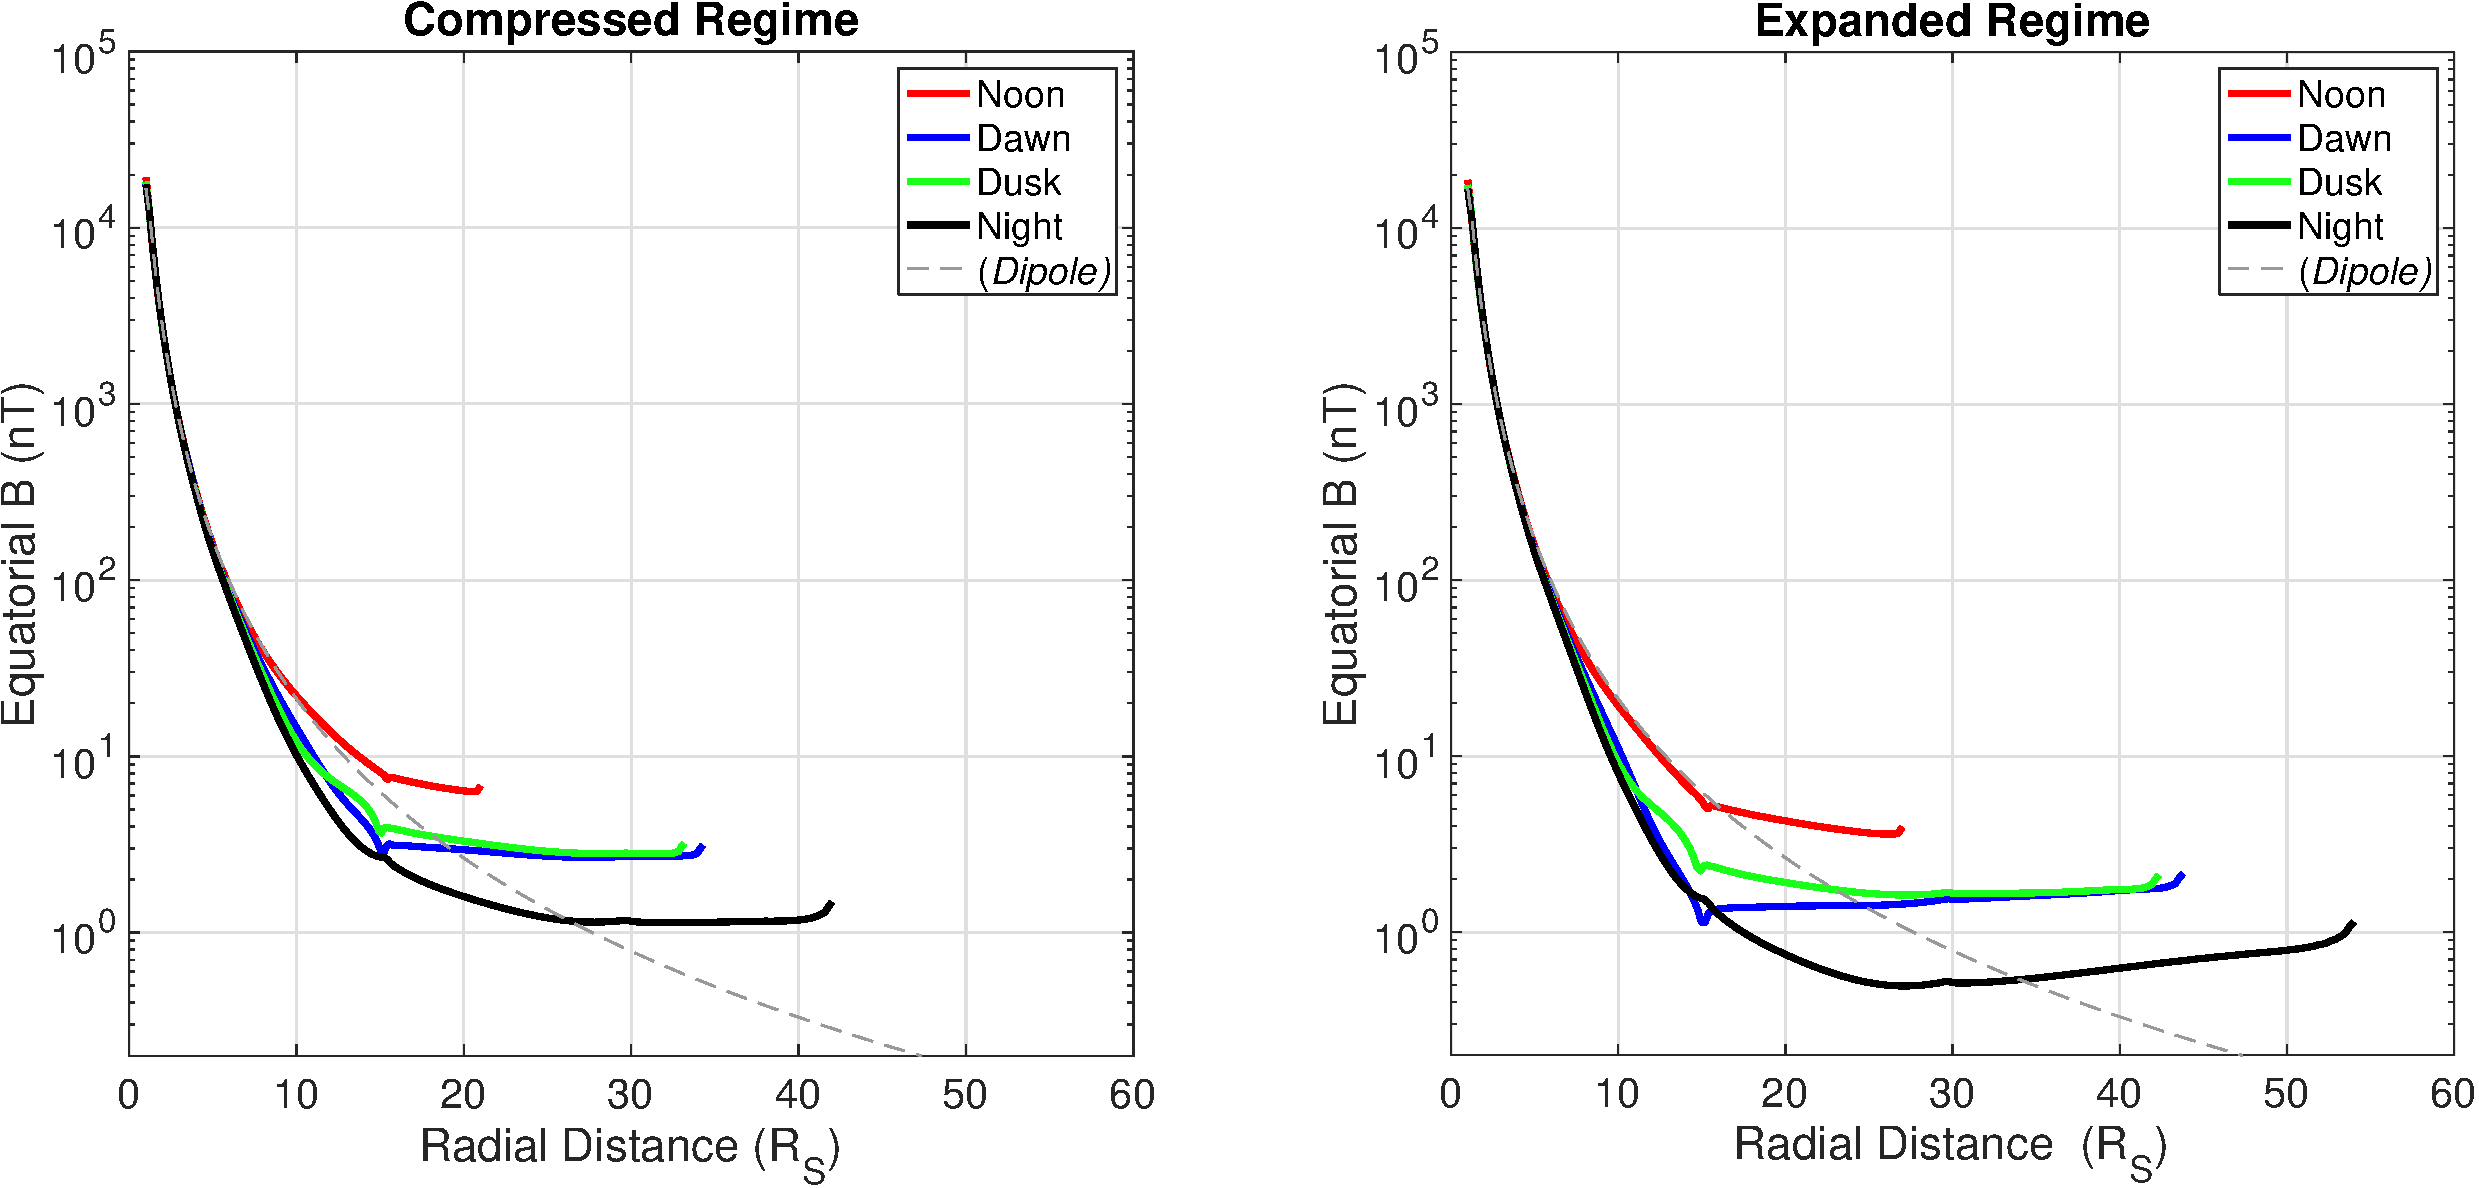
\includegraphics[width=0.8\textwidth]{LTsectors/eqBfield.pdf}
\caption[Model equatorial profiles of magnetic field strength $B$ for different local time sectors, for compressed and expanded regimes.]{Equatorial profiles of total magnetic field strength $B$ with radial distance for each local time sector as shown by the colour, for both the compressed (a) and expanded (b) regimes. On each plot a profile for a dipole magnetic field is shown in dashed grey for comparison.}
\label{LTsectors:fig:eqBfield}
\end{figure}

For the dayside (noon) models, we can see that the magnetic field is approximately dipolar in the inner ($\lesssim\SI{10}{R_S}$) magnetosphere, and falls more slowly with radial distance than a dipole in the middle ($10\lesssim\rho\lesssim\SI{15}{R_S}$) and outer magnetosphere. This behaviour broadly corresponds to a more `disc-like' magnetic field structure compared to a dipole, and appears for a more significant range in radial distance for the expanded noon model. Similar behaviour has been found in observational studies of Saturn's magnetosphere. For example \citet{arridge2008} showed that the dayside magnetospheric magnetic field was approximately dipolar when the system was compressed, but more disc-like when expanded, particularly beyond a sub-solar magnetopause radius of ${\sim}\SI{23}{R_S}$. Results of ring current modelling from \citet{bunce2008} found a similar result. 

For the larger dawn, dusk, and night sector models, the model magnetic field strengths are lower than the corresponding dipole field in the inner magnetosphere, and greater in the outer magnetosphere. This too is in line with \textit{in situ} observations of Saturn's magnetosphere, such as \citet{delamere2015}, who analysed equatorial current sheet crossings using \textit{Cassini} MAG data, in order to demonstrate how the equatorial magnetic field varies with radial distance in different local time sectors. There is also a small dawn-dusk asymmetry in the magnetic field strengths in our model, with the dusk sector profile persistently higher than the dawn. This is likely a consequence of force balance, with the slightly higher hot plasma pressure in the dusk sector requiring a greater magnetic curvature force to balance it. This is interesting to note, as such a small asymmetry in field strength would be unlikely to reveal itself in observational studies of Saturn's magnetosphere, especially due to the relatively poor sampling of the dawn sector equatorial magnetosphere by the \textit{Cassini} spacecraft over its mission.

Looking at the day-night asymmetry in more detail, in Figure~\ref{LTsectors:fig:carbarycomparison} we show the magnetic field structure for our noon and nightside magnetodisc models, for the compressed (top panel) and expanded (bottom panel) regimes. For comparison, we include in red an empirical magnetic field model from a recent study by \citet{carbary2018}. In that study the author binned magnetic field observations from the entire \textit{Cassini} mission into two local time sectors, dayside and nightside, and fit these using polynomial functions of latitude in order to derive a simple analytical model of Saturn's meridional magnetic field lines. \citet{carbary2018} accounted for seasonal warping of the current sheet via a coordinate transformation, although the polynomial functions still include terms that enable asymmetry across the rotational equator. However unlike in this study, the \citet{carbary2018} did not account for a change in external solar wind conditions, and so we have reproduced the same model output from \citet{carbary2018} in the top and bottom panels. We can see that the overall magnetic field structures in our models are similar to those of the \citet{carbary2018} model, in particular the expanded $\SI{27}{R_S}$ dayside model, and the compressed $\SI{42}{R_S}$ nightside model. In addition, the somewhat blunt, `blockish' shape of the dayside field lines in the \citet{carbary2018} model are somewhat accentuated by the polynomial representation the author used, with the original traces of field lines presented showing a structure even more similar to our models presented here. Only our expanded nightside model shows a magnetic field structure that is significantly more disc-like than the \citet{carbary2018} analytical model, suggesting that perhaps a magnetodisc radius of $\SI{54}{R_S}$ is somewhat too extreme to accurately characterise the typical midnight magnetosphere. However in general the agreement is very good, suggesting our models can characterise the overall structure of the magnetospheric magnetic field at different local times, provided the disc radius is chosen appropriately. Also, we should note that here we are comparing specifically our noon (LT 03:00-09:00) and night (LT 21:00-03:00) sector models, with the \citet{carbary2018} models which correspond to wider, 12 hour local time regions. Therefore to more accurately represent (for example) the entire dayside for a more direct comparison, we would need to consider some combination of our noon, dawn and dusk sector model outputs.

\begin{figure}
\centering
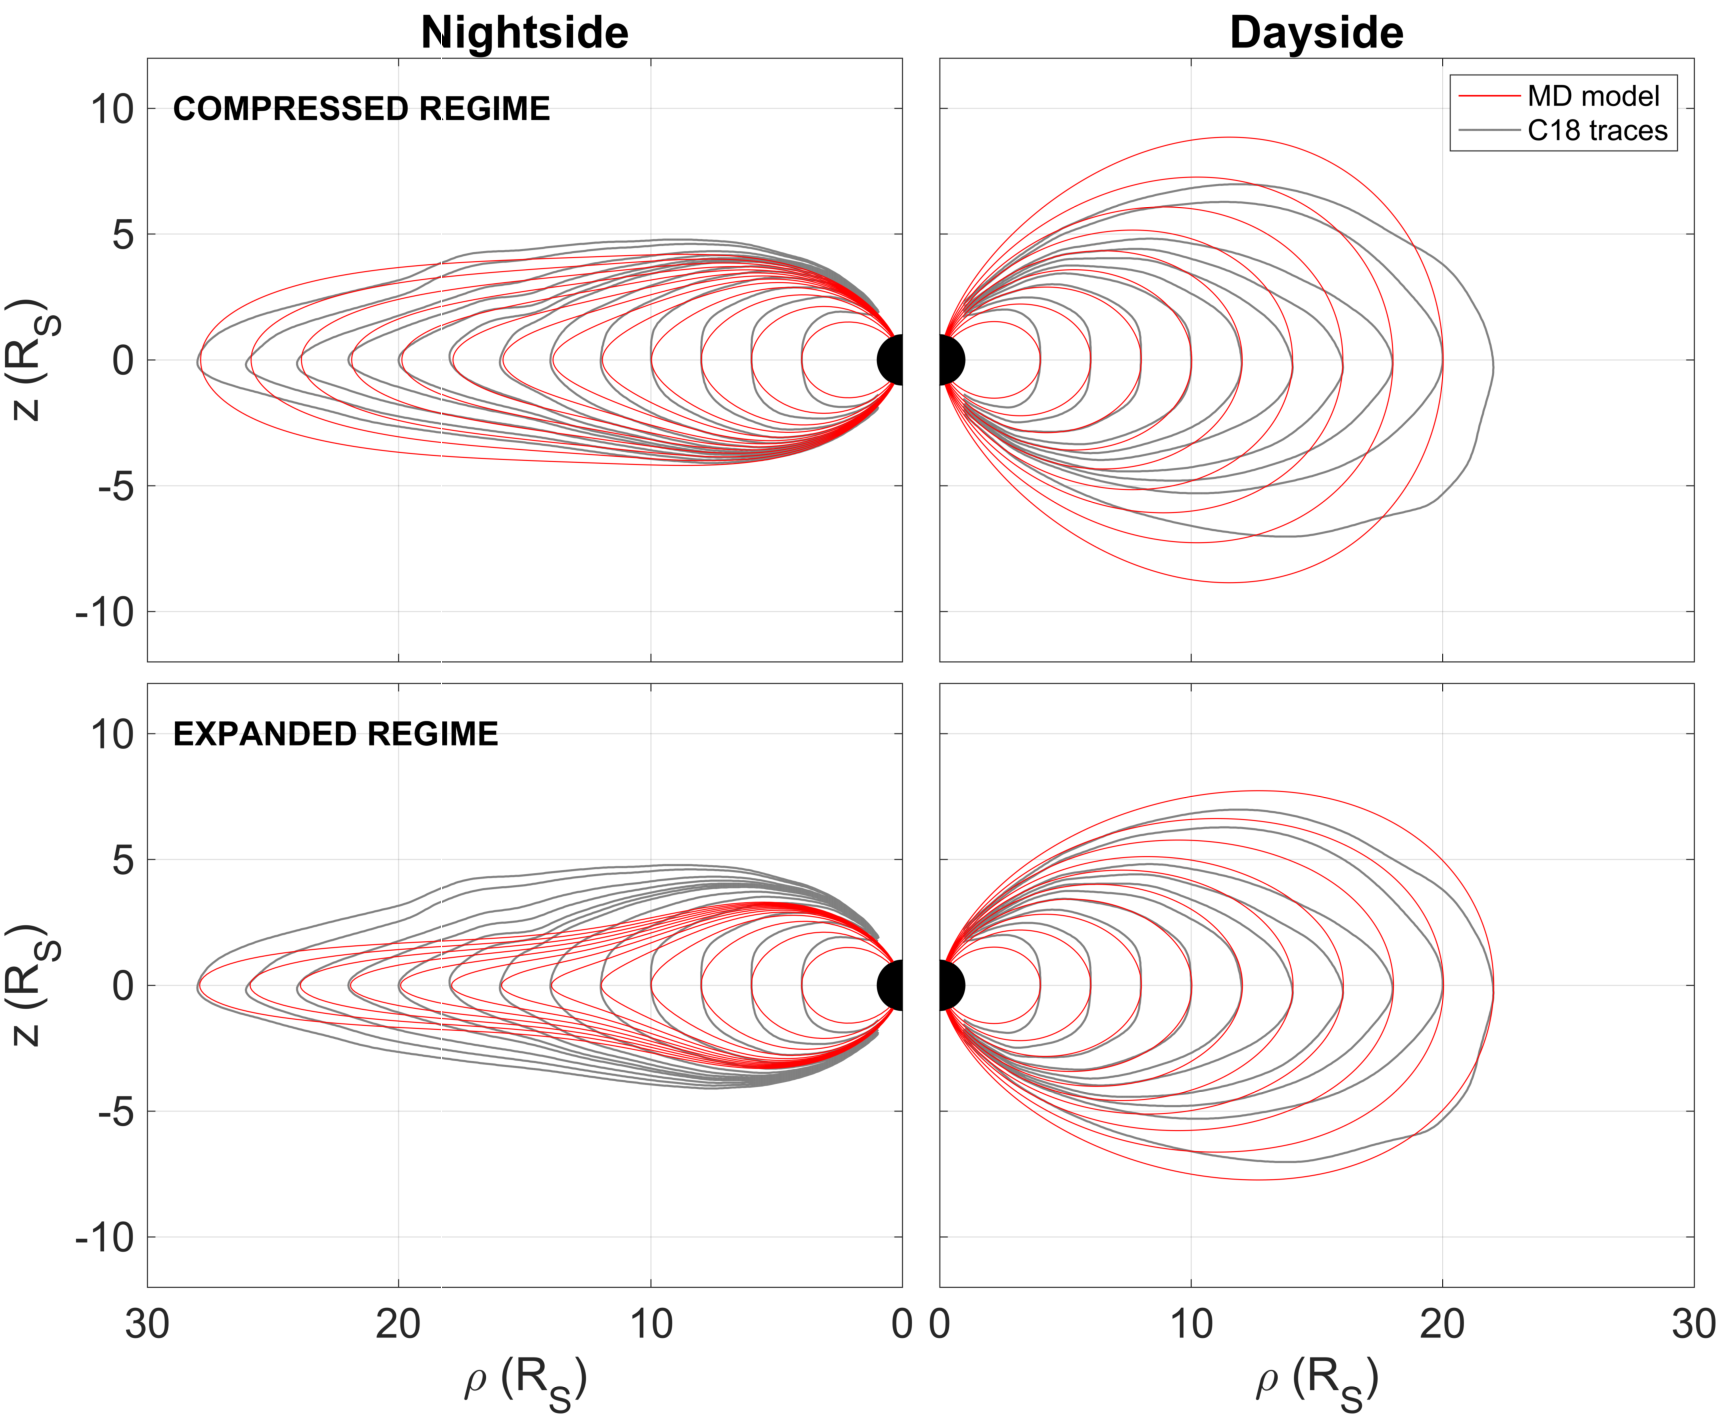
\includegraphics[width=0.7\textwidth]{LTsectors/carbarycomparison.pdf}
\caption[Model magnetic field lines for the dayside and nightside models, for the compressed and expanded regimes, compared to \citet{carbary2018} results.]{A comparison of model magnetic field lines from \citet{carbary2018} and this study. In grey are shown polynomial fits to binned \textit{Cassini} magnetometer meridional magnetic field observations from \citet{carbary2018} (top and bottom panels an exact reproduction). In red are shown magnetic field lines from the noon and nightside models presented in this study, for the compressed (top panel) and expanded (bottom panel) regimes, for L shells to match those of the \citet{carbary2018} study.}
\label{LTsectors:fig:carbarycomparison}
\end{figure}

In order to investigate more just how `disc-like' the magnetic field is in each local time sector, we use a visualisation technique employed in \citet{bunce2008}, where for each model we bound regions of the magnetosphere where the local magnetic field direction lies within $\SI{30}{\degree}$ of the equatorial plane, such that the field lines are approximately parallel to the equatorial plane. The results are shown in Figure~\ref{LTsectors:fig:discyness}, and the reproduction of the most lower latitude of the bounding lines are shown in Figure~\ref{LTsectors:fig:discyness2}. The magnetic field structure for each model is also shown in black, to further illustrate how this method characterises the `discy-ness' of the magnetic field structures. These figures show that, as expected, the larger magnetodisc models have significantly more disc-like magnetic field structures in the middle magnetosphere, than the smaller, more dipolar models. As discussed in the introduction, this was observed in previous studies such as \citet{arridge2008,achilleos2010a,sorba2017} and is a result of how the overall force-balance within the magnetosphere changes with system size, in terms of the dominant magnetic and plasma related forces. 

\begin{figure}
\centering
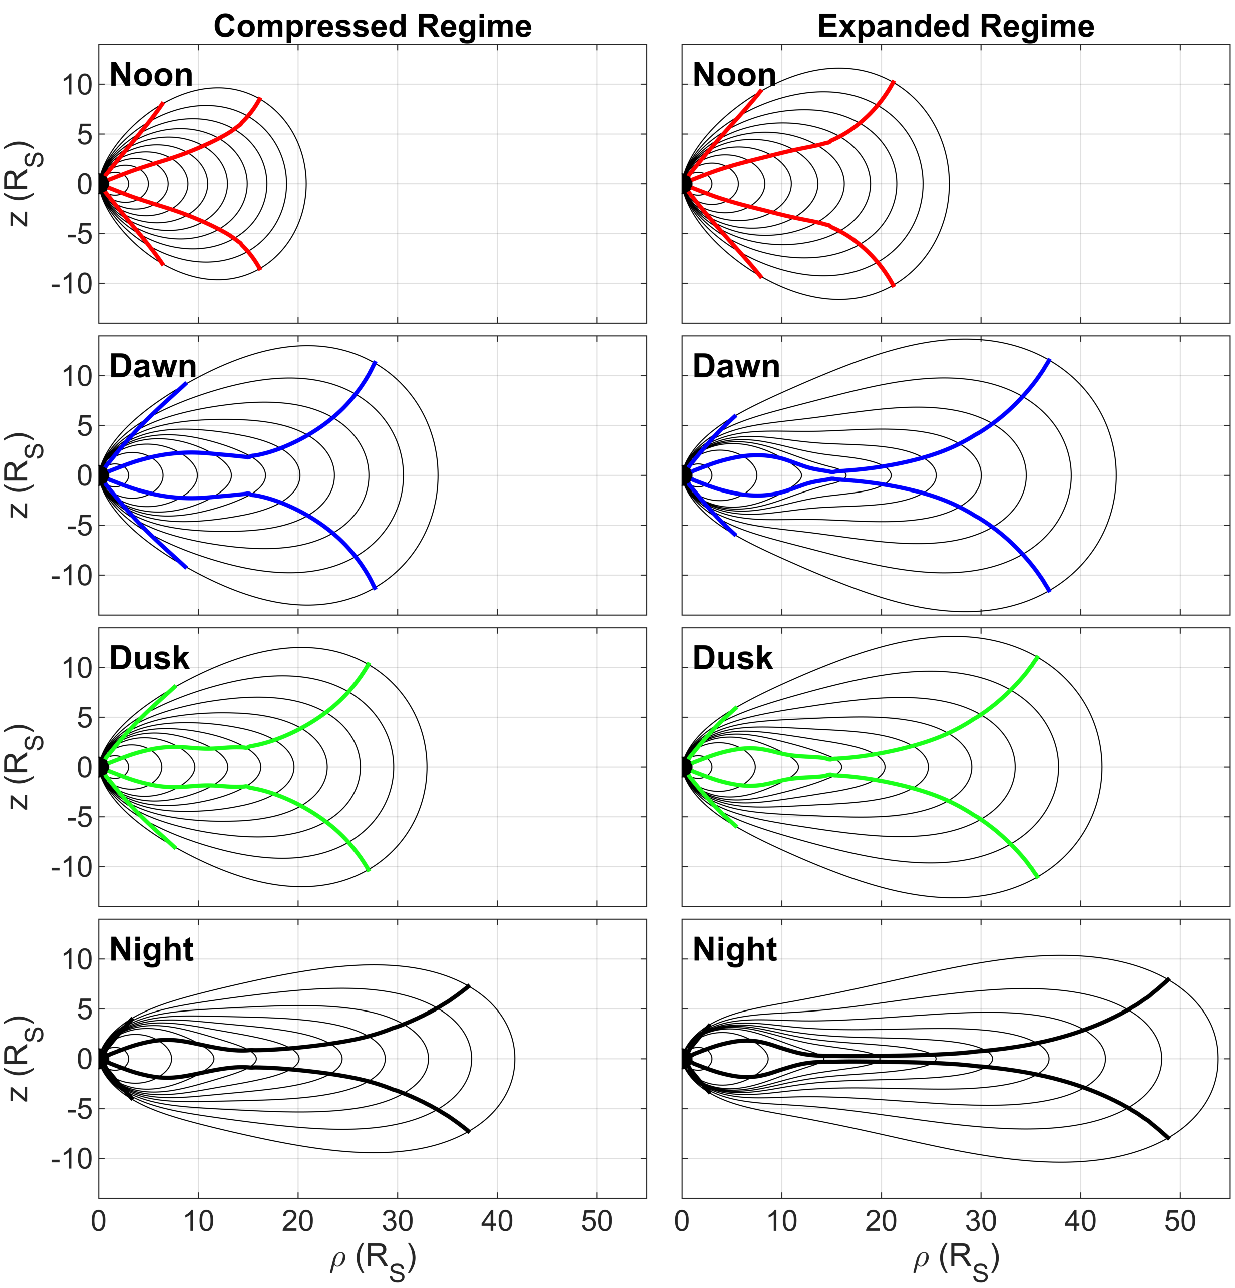
\includegraphics[width=0.8\textwidth]{LTsectors/discyness.pdf}
\caption[Model magnetic field structures for different local time sectors, with bounding lines showing regions where the magnetic field direction is within $\SI{30}{\degree}$ of the equatorial plane.]{The magnetic field structure for each magnetodisc model for the compressed (left column) and expanded (right column) regimes, shown by the solid black lines. Superposed in colour for each model are pairs of lines in each hemisphere which bound regions where the local magnetic field direction lies within $\SI{30}{\degree}$ of the equatorial plane.}
\label{LTsectors:fig:discyness}
\end{figure}

\begin{figure}
\centering
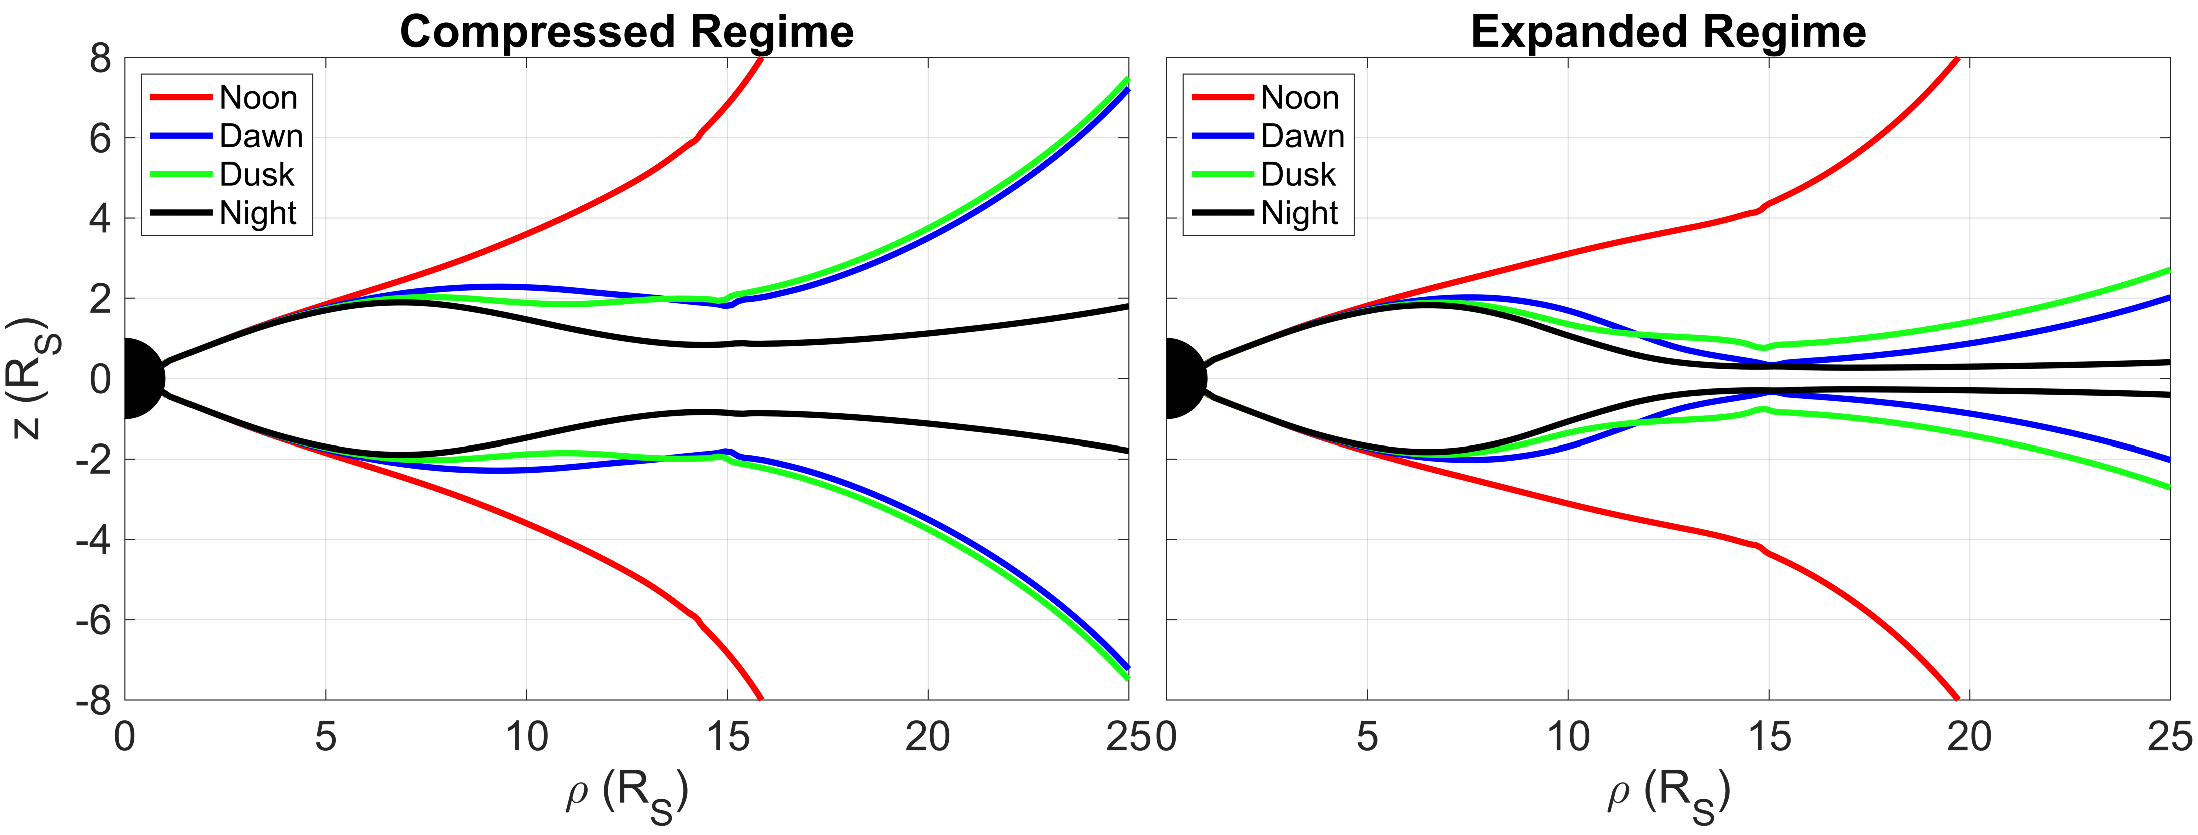
\includegraphics[width=0.8\textwidth]{LTsectors/discyness2.pdf}
\caption[Reproduction of the lower latitude bounding lines from Figure~\ref{LTsectors:fig:discyness}.]{Reproduction of the more equatorward coloured lines from Figure~\ref{LTsectors:fig:discyness}, for each local time sector model, for compressed (left) and expanded (right) regimes. These represent the low latitude boundaries of regions where the local magnetic field direction lies within $\SI{30}{\degree}$ of the equatorial plane.}
\label{LTsectors:fig:discyness2}
\end{figure}

In addition, from Figure~\ref{LTsectors:fig:discyness2} in particular, it can be seen that, for the compressed regime, the dusk sector has a slightly thinner and more disc-like magnetodisc structure in the middle magnetosphere than the dawn sector, as shown by the bounding lines being more equatorward for the dusk model (shown in green). This effect is likely due to the local enhancement of the ring current in the dusk sector due to the increased hot plasma pressure, which causes a more extreme perturbation from a dipolar magnetic field. This was also discussed in the introduction, and observed in \citet{achilleos2010b,sorba2017}. Note that this `thinning' of the disc is not the same as thinning of the \textit{plasma} sheet, which is made up of both hot and cold plasma populations. While the \textit{current} sheet and associated \textit{cold} plasma sheet thins, the hot plasma is actually more populous for the thinner, dusk model, and the associated hot plasma pressure is constant along magnetic field lines. As described in \citet{sergis2011,arridge2009b} the current sheet, a predominantly magnetic structure, has been observed to be thinner than the plasma sheet it is embedded in, and the plasma sheet itself can have different thicknesses in different particle energies and species.

For the expanded regime, it can be seen in Figure~\ref{LTsectors:fig:discyness2} that the opposite relationship is true, and that in the middle and outer magnetosphere, the dawn sector magnetic field has a thinner and more disc-like structure (shown in blue). This is likely due to the increased influence of the dawn-dusk asymmetry in effective magnetodisc radius for the expanded regime, as a larger magnetopause radius also promotes a more disc-like structure. For the expanded regime, the dawn magnetopause is $\SI{1.5}{R_S}$ greater than the dusk, compared to $\SI{1.1}{R_S}$ for the compressed regime. It is interesting that this transition in dominant behaviour occurs across this compressed-expanded regime threshold. These results suggest that the asymmetries in magnetopause radius and hot plasma content have comparable influence on the global magnetic field structure in those local time sectors. In addition, the expanded system models may be more strongly influenced by the assumption we made that the product of flux tube volume and hot plasma pressure is constant beyond $\SI{15.5}{R_S}$, as described in Section~\ref{LTsectors:sec:hotP}, as this region is by definition more extended for the expanded system models, where $R_\mathrm{D}$ is greater. We hope to relax this assumption with an updated parameterisation of the hot plasma pressure beyond $\SI{15.5}{R_S}$ in a future study.

In the aforementioned study by \citet{delamere2015}, the authors find significantly more incidences of `critically thin' equatorial current sheet encounters in the dusk sector than the dawn sector, even when accounting for the sampling bias of \textit{Cassini} (which spent more time in the dusk sector). This is therefore more in line with our picture of the compressed regime, with a thinner current sheet on the dusk side due to the influence of the increased hot plasma pressure. In contrast, in a study from \citet{jia2016}, based on MHD simulations of Saturn's magnetosphere from \citet{jia2012b}, they find the opposite behaviour, with a significantly thinner current sheet and more radially stretched magnetic field lines in the dawn sector, which is also observed at Jupiter~\citep[e.g.][]{khurana2004}. This may be understood, as that the simulations of \citet{jia2012b} do not include a suprathermal plasma population, and so the effect of the enhanced hot plasma population on the dusk side is not captured in their study. In addition, it was suggested by \citet{pilkington2015b} that this absence of suprathermal plasma in the \citet{jia2012b} models may cause their models to slightly overestimate the dawn-dusk asymmetry in magnetopause radius, which predict a mean asymmetry of $\SI{2.6}{R_S}$, compared to $\SI{1.6}{R_S}$ for the \citet{pilkington2015b} empirical model. Therefore the results of \citet{jia2016} may be more strongly influenced by this asymmetry in magnetopause radius, which, as discussed, provides a thinner and more disc-like current sheet in the dawn sector. However, their MHD models do account for plasma acceleration, and azimuthal asymmetry in the magnetic field, which the force-balance models presented in this study do not. Therefore some dawn-dusk asymmetry in these factors may also influence current sheet thickness in ways that our model cannot capture.

\subsection{Ionospheric Field Line Mapping and Azimuthal Current Density} 
We discussed in Section~\ref{LTsectors:sec:intro} varying hot plasma content and magnetopause radius can both affect the mapping of magnetic field lines from the equator to the ionosphere, due to a reconfiguration of the magnetospheric magnetic field structure. It is therefore important to consider how this ionospheric mapping varies for different local time sectors.

The inner boundary of our magnetodisc model is located at a radial locus of $\SI{1}{R_S}$ where $\si{R_S}=\SI{60268}{\km}$, specifically the \textit{equatorial} radius of Saturn at 1 bar atmosphere level. This is greater than the \textit{polar} radius at 1 bar, as Saturn is oblate. Our model therefore does not directly calculate the magnetic field in the polar ionospheric regions, as these regions are closer to the planet than the inner boundary of our model. Also, our model assumes a centreed dipole planetary magnetic field. Therefore we need to account for the oblate spheroid shape of the planet, the altitude of the ionosphere, and effective offset of the planetary dipole in our ionospheric mapping calculations. We do this by calculating the magnetic potential $\alpha$ (see discussion in Section~\ref{intro:sec:forcebalancemodel}) for a dipole magnetic field with origin offset northwards by $z_\mathrm{off}=\SI{0.0466}{R_S}$ \citep{dougherty2018}, along a surface $\SI{1100}{km}$ altitude above an oblate spheroid with equatorial radius $\SI{60268}{\km}$ and polar radius $\SI{54364}{\km}$ \citep{seidelmann2007}. The ionospheric altitude of $\SI{1100}{km}$ was chosen following studies from \citet{gerard2009,stallard2012} and others. As the magnetic potential $\alpha$ is constant along a given magnetic field line by definition, we can then map equatorial values of $\alpha$ to the oblate ionospheric surface in order to estimate the realistic colatitude at which the magnetic field lines would pierce the northern and southern polar ionospheres.

The resulting values are shown in Figure~\ref{LTsectors:fig:fieldlinemapping}, with northern hemisphere values shown by solid lines and southern hemisphere counterparts shown by dotted lines. All values shown in Figure~\ref{LTsectors:fig:fieldlinemapping} are also provided in tables in the Supporting Information to \citet{sorba2019}. Also shown by the coloured solid circles with error bars are the average locations and widths of the main auroral oval for noon, dawn and dusk local time sectors respectively, estimated from a statistical study of multiple Hubble Space Telescope (HST) observations of the UV aurora in the southern hemisphere from \citet{badman2006}. As these observations were of the southern hemisphere only, they should be compared with the dotted lines of the model outputs.

\begin{figure}
\centering
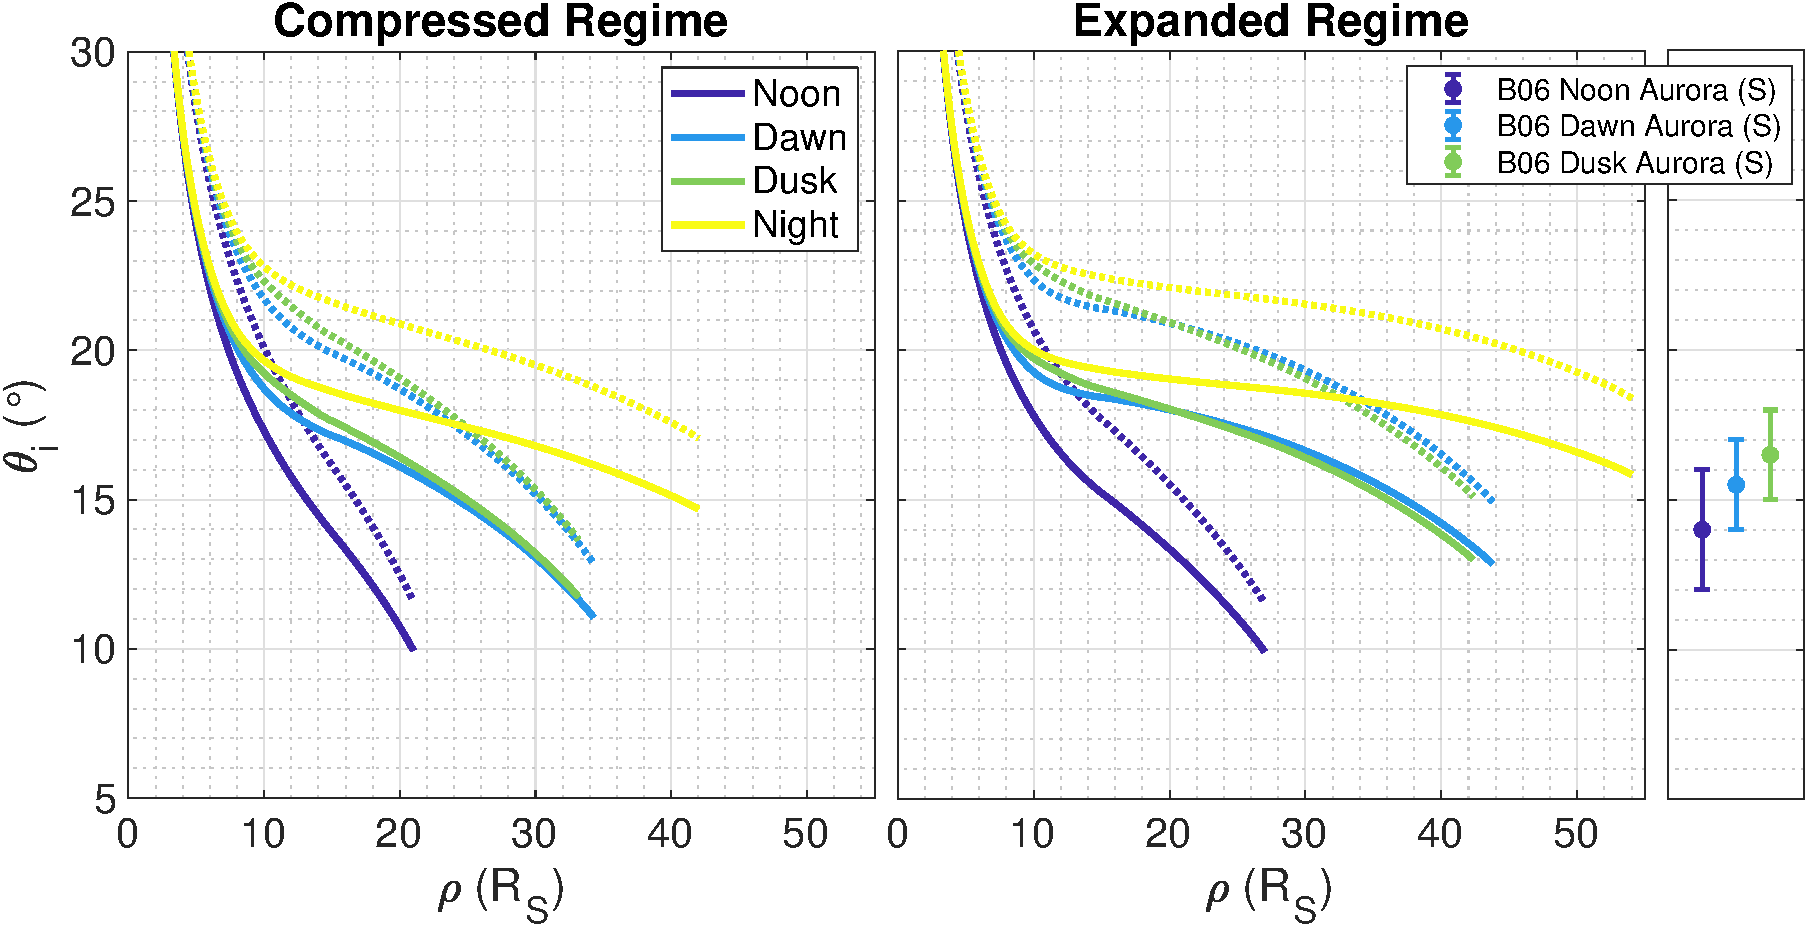
\includegraphics[width=0.9\textwidth]{LTsectors/fieldlinemapping.pdf}
\caption[Model equatorial profiles of field line mappings from the equator to the ionosphere, for different local time sectors, for the compressed and expanded regimes.]{Equatorial profiles showing the mapping of magnetic field lines from the equatorial plane to the northern (solid lines) and southern (dotted lines) ionospheres, with local time sector shown by the colour. Ionospheric colatitude $\theta_\mathrm{i}$ is measured relative to the northern pole for northern hemisphere values, and the southern pole for southern hemisphere values. Also shown by the solid circles with error bars are median locations and widths of the main auroral oval in the southern hemisphere for different local time sectors as shown by the colour, from a statistical study by \citet{badman2006}. Model values shown here are provided in tables in the Supporting Information to \citet{sorba2019}.}
\label{LTsectors:fig:fieldlinemapping}
\end{figure}

It can clearly be seen that there is significant variation in ionospheric mapping of field lines for different local time sectors. In particular, the locations of the open-closed field line boundary (OCFLB), shown by the colatitude of the most radially distant point for each profile, vary greatly between sectors. We can see that the OCFLB maps to more polar regions in the noon sector, with ${\sim}\SI{10}{\degree}$($\SI{11.5}{\degree}$) for the northern (southern) hemisphere, than for the night sector, with ${\sim}\SI{15.5}{\degree}$($\SI{17.5}{\degree}$) for the northern (southern) hemisphere. This behaviour is qualitatively in agreement with the results of \citet{carbary2018}, who find corresponding values of ${\sim}\SI{13}{\degree}$($\SI{16}{\degree}$) for the dayside, and ${\sim}\SI{16}{\degree}$($\SI{18}{\degree}$) for the nightside, using a data-based magnetic field model. Our noon sector values are somewhat lower than the dayside values of \citet{carbary2018}; however, if we were to consider some combination of our noon, dawn and dusk values to represent the entire dayside hemisphere, for a more appropriate comparison, they would likely be in better agreement. This is because the values for dawn and dusk are both higher than the noon value alone.

In addition, for the compressed regime in particular, we find a slight dawn-dusk asymmetry in the location of the OCFLB, with the dusk location around $\SI{1}{\degree}$ equatorward of the dawn location. It can be seen on close inspection of Figure~\ref{LTsectors:fig:fieldlinemapping} that this asymmetry is mainly due to the small asymmetry in magnetopause radius in these models, rather than the influence of the hot plasma pressure profiles on the magnetic field structure. This is evident as the two profiles are broadly coincident in the outer magnetosphere until the dusk model terminates at $\rho=\SI{33.2}{R_S}$, in comparison to dawn's $\SI{34.3}{R_S}$ (see Table~\ref{LTsectors:tab:modelparams}). It is interesting to note that this relationship is qualitatively similar to that observed by \citet{badman2006}, who found that on average the main auroral oval in the dusk sector was located ${\sim}\SI{1}{\degree}$ equatorward of the aurora in the dawn sector, in the southern hemisphere. Furthermore, the dawn aurora was observed to be ${\sim}\SI{1.5}{\degree}$ equatorward of the noon auroral location in \citet{badman2006}. This is approximately the same as the difference in the OCFLB we observe between our noon and dawn models for the compressed regime, southern hemisphere values, as shown in the first panel of Figure~\ref{LTsectors:fig:fieldlinemapping} (although the difference is significantly higher for the expanded regime). Such a comparison supports the hypothesis from this and other studies, that the main auroral oval may map to regions in the outer equatorial magnetosphere, within a few $\si{R_S}$ of the OCFLB. In addition, a later study by \citet{badman2011} of Saturn's infrared aurora found that the nightside main oval was persistently ${\sim}\SI{2}{\degree}$ equatorward of the dayside, in line with the aforementioned day-night asymmetry we observe in our OCFLB. It is interesting to note that this agreement is achieved despite the shielding field associated with the UCL/AGA model, discussed in Section~\ref{LTsectors:sec:adaptations}, being a less accurate approximation in the higher latitude regions, beyond around $\SI{50}{\degree}$ latitude \citep{caudal1986}.

Now comparing the results for the compressed and expanded regimes, we see that the differences between the profiles are not as extreme as the differences between local time sectors. This suggests that variations in external solar wind conditions do not have a significant impact on the magnetic mapping between ionosphere and the equatorial disc. In particular for the noon sector, the profiles for the compressed and expanded regimes are very similar, with near coincident locations of the OCFLB, and similar regions of the equatorial magnetosphere mapping to similar values of $\theta_\mathrm{i}$ in each case. For example, the equatorial radial distance corresponding to the outer one-third of the noon sector magnetosphere for each regime, maps to roughly the same $\theta_\mathrm{i}$ for each case, ${\sim}\SI{14}{\degree}$ in the north, and ${\sim}\SI{16.5}{\degree}$ in the south. A similar result was found in \citet{bunce2008}, who used an adapted ``CAN'' type \citep{connerney1981b,connerney1983} ring current model from \citet{bunce2007} to investigate how ionospheric mapping varied with system size in the noon sector magnetosphere. They found only a very modest variation with system size, for a noon magnetopause radius range of $16-\SI{26}{R_S}$, comparable to the range in this work. \citet{bunce2008b} then used the results of this modelling, in combination with HST observations of the UV aurora and \textit{Cassini} data, to show that the noon aurora are indeed likely to lie near the boundary between open and closed magnetic field lines. These authors go on to suggest that the quasi-continuous main auroral oval corresponds to the OCFLB at other local time sectors, in line with our interpretation here. Combining results for all local time sectors and compressed/expanded regimes, we find a mean location of the OCFLB equal to $\SI{12.4}{\degree}$ in the north and $\SI{14.4}{\degree}$ in the south. This is comparable to recent results from a \textit{Cassini} multi-instrument study from \citet{jinks2014}, who find corresponding values of $\SI{13.3}{\degree}$ in the north and $\SI{15.6}{\degree}$. In that study, the majority of observations are from the post-midnight sector where we expect the OCFLB to be more equatorward, which may explain why their average values are a little higher than ours.

When interpreting ionospheric-equatorial magnetic mappings, it is also pertinent to consider how the total current density varies with radial distance in the equatorial magnetosphere. Predictions for total azimuthal current density at the equator for each local time sector model, for compressed and expanded regimes, are shown in Figure~\ref{LTsectors:fig:currentdensity}. (Note that as the magnetodisc model is azimuthally axisymmetric, and hence used here to represent individual local time sectors separately, radial currents are not directly predicted.) Superimposed on each plot is a representative profile with azimuthal current density inversely proportional to cylindrical radial distance $\rho$, as is the case for CAN type ring current model constructions from \citet{connerney1981b,connerney1983}.

\begin{figure}
\centering
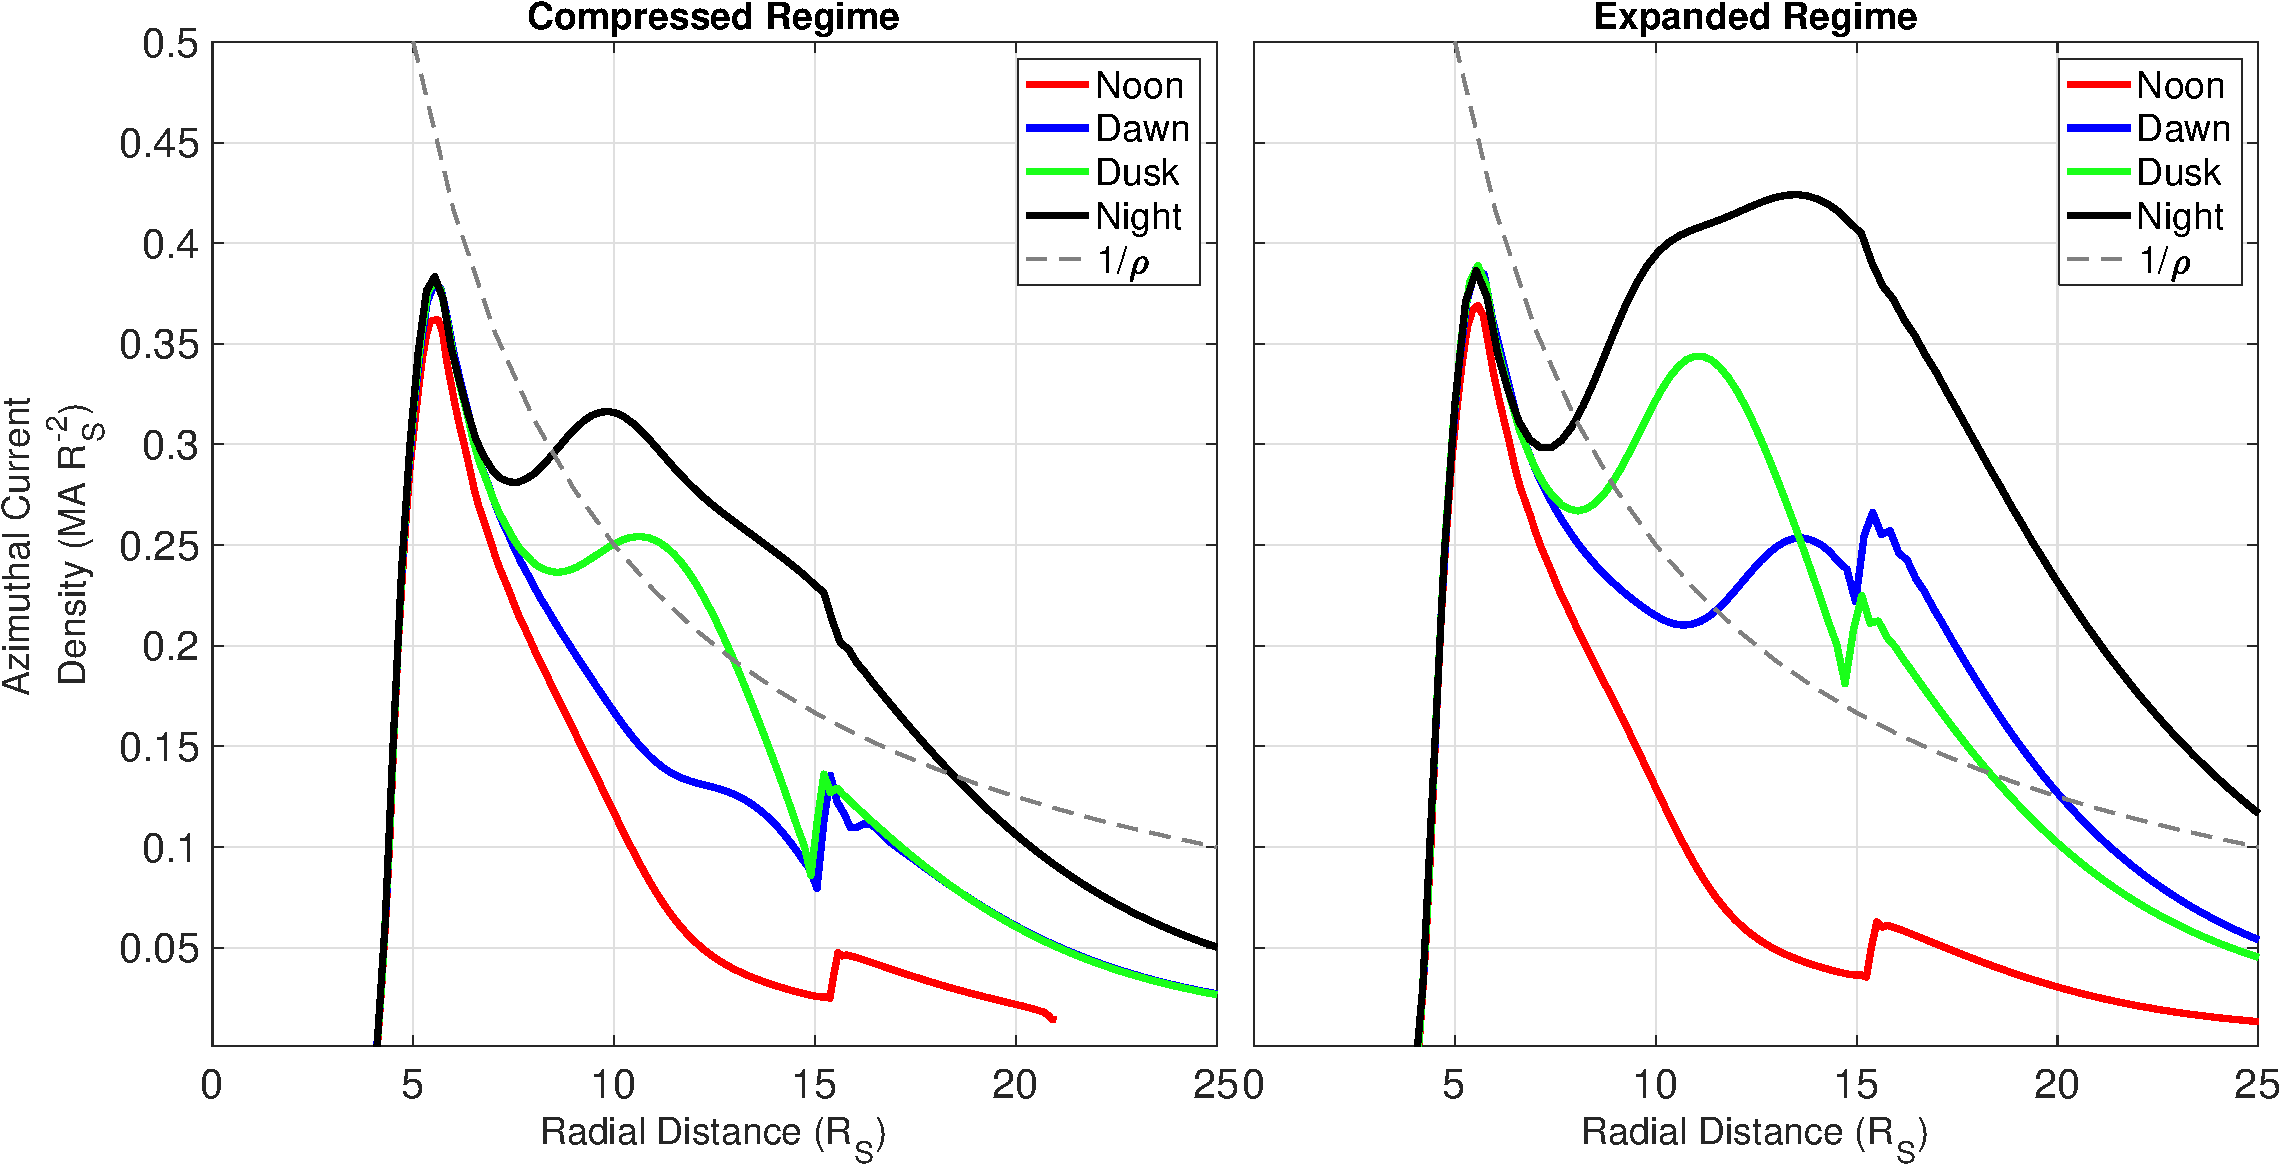
\includegraphics[width=0.8\textwidth]{LTsectors/currentdensity.pdf}
\caption[Model equatorial profiles of azimuthal current density for different local time sectors, for compressed and expanded regimes.]{Profiles of equatorial azimuthal current density with radial distance, for each local time sector model as shown by the colour, for compressed (left) and expanded (right) regimes. The grey dashed line shows a representative profile with current density inversely proportional to radial distance, as for a \citet{connerney1981b, connerney1983} style ring current model.}
\label{LTsectors:fig:currentdensity}
\end{figure}

We can clearly see significant dawn-dusk and noon-night asymmetry in the current density profiles, with higher magnitudes for the dusk and night sector models, for both the compressed and expanded regimes. This is due to the similar relationship between the different input equatorial hot plasma pressure profiles for each local time sector, shown in Figure~\ref{LTsectors:fig:hotPpolys}, enhancing the component of the ring current associated with the hot plasma pressure gradient. In addition, the underlying magnetic field structure, and the centrifugal force on the cold plasma, both influence the current density profile via force-balance as in equation~(\ref{intro:eq:forcebalance}). This helps explain the significant difference in all profiles between the compressed and expanded regimes, with larger models having in general higher magnitude predicted azimuthal currents, due to lower magnetic field strengths at the equator as shown in Figure~\ref{LTsectors:fig:eqBfield}. The nightside models in particular have much higher predicted current densities than all other sector models for this reason. Similar results were also shown in a study by \citet{jia2012a}; in that study, the authors presented results of MHD simulations of Saturn's magnetosphere and ionosphere, and found that the predicted azimuthal current density had a persistent local time asymmetry, being higher by a factor of ${\sim}2{\--}3$ on the nightside than at other local times. In addition, it is interesting to note that for the expanded regime, the region $\rho \approx {13}{R_S}$ where the current density at dawn surpasses the current density at dusk, is almost coincident with the region where the dawn magnetic field structure becomes more disc-like than dusk, as shown in Figure~\ref{LTsectors:fig:discyness2}. This further illustrates the relationship between ring current activity and magnetodisc magnetic field structure.

From Figure~\ref{LTsectors:fig:currentdensity} we can also see that for all local time sectors, beyond the local maximum region, the equatorial current density falls more quickly than the $1/\rho$ decrease predicted by a CAN type ring current model. Similar behaviour was also found in the observational study from \citet{sergis2017}, who used \textit{Cassini} MAG, MIMI and CAPS observations to make estimates of equatorial azimuthal density profiles, and found local maxima for each sector profile in the radial range ${\sim}7-\SI{13}{R_S}$, followed by a fast decay with radial distance. This suggests that the more complex ring current structure enabled by the modified UCL/AGA model used in this study may be more appropriate at characterizing the true structure of Saturn's equatorial current sheet than a CAN type model. However both types of model give similar predictions for the magnetic field away from the edges of the CAN disc, as discussed in \citet{achilleos2010a}.

\section{Summary and Conclusions of this Chapter} \label{LTsectors:sec:conclusions}
In this study we have used the 2-D, force-balance UCL/AGA model from \citet{achilleos2010a} to describe the typical, equilibrium conditions of Saturn's magnetosphere at four different local time sectors. We have used equatorial profiles of hot plasma pressure at different local times from \citet{sergis2017}, and a magnetopause surface model from \citet{pilkington2015b}, to investigate how global hot plasma content and system size influence the magnetospheric structure at different local times.

We have found that, as expected, there is significant day-night asymmetry in the magnetic field structure of the magnetosphere, and that this is mainly due to the large asymmetry in magnetopause radius between day and night. We also find a small dawn-dusk asymmetry in the magnetic field structure, with both the hot plasma content and mangetopause radius having comparable influence. For the compressed regime, where the magnetosphere is under high solar wind dynamic pressure conditions, we find that the dusk sector magnetic field is more disc-like due to the influence of the increased hot plasma pressure in that sector. Meanwhile for the expanded regime we find the opposite is true, and that the dawn magnetic field is more disc-like, due to the larger magnetopause radius at dawn for this regime. Importantly, we also find significant differences in how equatorial magnetic field lines map to the polar ionosphere for the different local time sector models, with field lines from the outer magnetosphere mapping to far more equatorward regions of the ionosphere on the nightside than the dayside. This result is useful in particular when interpreting auroral observations at Saturn's ionosphere and attempting to ascertain their origins in the magnetosphere. These results may also be useful for future studies looking at local time variations in other magnetospheric properties, such as current sheet thickness.

The simplicity of the modelling approach used in this work means that many magnetospheric properties can be easily compared between different local time sectors. However a consequence of this is that any dynamical behaviour, such as reconnection events or plasmoids, cannot be directly captured. In addition, due to the assumed axisymmetry of each model, we cannot investigate the influence of any observed local time asymmetry in azimuthal phenomena. For example, a non-negligible dawn-dusk asymmetry in the azimuthal `bend-back' of magnetic field lines in the direction opposite to planetary rotation has been observed, with more substantial bend-back in the dawn sector than the dusk sector \citep[e.g.][]{delamere2015}. This may affect our assumptions of how magnetospheric plasma properties vary with radial distance, such as the angular velocity, which in turn influences our estimates of centrifugal force. In \citet{jia2016}, the authors offer a formulation for how the force balance assumption of equation~(\ref{intro:eq:forcebalance}) could be modified to account for a local time variation in radial outflow of plasma. While a preliminary investigation suggests this approach would not have a significant impact on our results, it would be worthwhile to investigate this further in a future study.

In summary, the study presented in this chapter shows that there is significant local time variation in the magnetic field structure of Saturn's magnetosphere. The equatorial current sheet thickness, current density and magnetic mapping to the ionosphere all vary depending on both local time and external solar wind pressure conditions, due to force balance within the magnetosphere in this study. Our results are useful for potential future studies looking to interpret a range of phenomena at Saturn, from reconnection events and plasmoids to auroral oval modulations. 
\chapter{Conclusions and Directions for Future Work}
\label{chap:conclusions}
\section{Summary of Main Conclusions of this Thesis}
\subsection{Impact of Magnetospheric System Size on Large-Scale Structure and Dynamics}
% TBD: 
In this thesis we have studied in detail how the large-scale structure and dynamics of Saturn's magnetosphere varies with system size. In Chapter~\ref{chap:compress}, we used the UCL/AGA model to investigate specifically how the compressibility of the magnetosphere varied with system size, and in Chapter~\ref{chap:LTsectors} we looked at how the large-scale structure varied at different system sizes across a range of local times. The size of the magnetosphere is in turn influenced by the upstream solar wind conditions; in Chapter~\ref{chap:intro} we discussed how the magnetopause location is determined to the first order by pressure balance between the solar wind dynamic pressure $D_\mathrm{P}$ and the internal magnetospheric plasma and magnetic pressures, and how $D_\mathrm{P}$ varies with both the density and speed of the solar wind plasma.

Our modelling results presented in Chapters~\ref{chap:compress} and \ref{chap:LTsectors} suggest that the large-scale structure of Saturn's magnetosphere is more disc-like when the system is expanded, beyond a sub-solar magnetopause radius of ${\sim}\SI{25}{R_S}$. This \textit{magnetodisc} configuration is associated with more radially stretched field lines in the middle magnetosphere near the equatorial plane around a thin equatorial current sheet, and a total magnetic field strength that falls more slowly with radial distance than a dipole magnetic field. If the system is compressed by increasing solar wind dynamic pressure, the magnetospheric magnetic field then reconfigures into a more dipolar structure, with a correspondingly thicker equatorial current sheet. 

Similar results were found in the empirical study by \citet{arridge2008}, based on \textit{Cassini} magnetic field observations. In that study, the authors surveyed \textit{Cassini} magnetometer data for current-sheet-like fields, and examined the distribution of observations that fit a certain set of criteria related to magnetic field strength and orientation, which corresponded to a stretched magnetic field configuration. They found that a significant magnetodisc structure only formed on the dayside when the system was expanded with a sub-solar radius beyond ${\sim}\SI{23}{R_S}$, and that for smaller systems, a magnetodisc only formed on the nightside and flanks. They suggested that this is due to the near-coincidence of the expected inner boundary of the magnetodisc based on a stress balance argument, and the nominal subsolar magnetopause, meaning the disc is prevented from forming under compressed conditions. This is in agreement with the results of the study by \citet{bunce2008}, based on models of the ring current from \citet{bunce2007}, which found that the magnetic moment of the ring current increases as the system expands, causing a more extreme distortion of the magnetospheric magnetic field in such conditions. This behaviour was also confirmed in the original UCL/AGA model study based on a comparison of two models calculated at different sizes \citep{achilleos2010a}.

In a steady-state system, we can consider this reconfiguration from a dipolar to a more disc-like structure in the context of the force balance in the rotating plasma of the magnetosphere, between the centrifugal force, plasma pressure gradient force and $\boldsymbol{J}\times\boldsymbol{B}$ Lorentz body force. In Section~\ref{intro:sec:plasmaforces} we showed how this Lorentz body force is equivalent to the sum of a magnetic pressure gradient force and a magnetic tension force. Near the equatorial plane, the main force acting radially inwards is the component of the magnetic tension force perpendicular to the magnetic field, which is proportional to $B^2/r_\mathrm{c}$ (where $r_\mathrm{c}$ is the magnetic field line radius of curvature). As the system expands, the magnetic field strength in the outer magnetosphere falls, and so in order for the magnetic tension force to balance the centrifugal and plasma pressure gradient forces acting radially outwards, the radius of curvature of the magnetic field lines must decrease. This corresponds to a more disc-like magnetic field structure, supported by a thin sheet of azimuthal current that extends far into the outer magnetosphere. 

This aspect of magnetodisc structure  becomes particularly important when investigating how Saturn's magnetospheric structure varies with local time. The nominal magnetodisc is significantly larger on the nightside and flanks of the magnetosphere than on the dayside, due to the interaction between the magnetosphere obstacle and the solar wind. In addition, recent results from \citet{pilkington2015b} suggest a small dawn-dusk asymmetry in the typical magnetopause radius. In Chapter~\ref{chap:LTsectors}, we presented results of a modelling study which suggested that this variation in system size did indeed influence the magnetic field structure at different local times, which in turn influences magnetic mapping between the equatorial disc and the ionosphere. We found that in particular the open-closed field line boundary mapped to more equatorial regions of the ionosphere for the nightside and flanks than on the dayside, with a small dawn-dusk asymmetry, which has impacts for interpreting ionospheric phenomena such as aurora, as discussed in that chapter.

In Chapter~\ref{chap:equinox} we used a family of UCL/AGA models calculated with different disc radii in the range $45{\--}\SI{55}{R_S}$, and organised with Saturnian `longitude',  to simulate a periodic thickening and thinning of Saturn's magnetospheric current sheet in response to the dual rotating magnetic perturbations. We found that, when combined with a geometrical model of a tilted and rippled current sheet surface, this model characterised well the observed periodic perturbations in the magnetic field measured by \textit{Cassini} in Saturn's outer magnetosphere. In particular we found that the meridional component of  the magnetic field was much better characterised when this thickness perturbation in the magnetodisc was included. This suggests that our approach of using an oscillating boundary location with a $\SI{10}{R_S}$ range in disc radius appropriately simulates the corresponding change in magnetodisc structure and current sheet thickness, although with caveats as discussed in Chapter~\ref{chap:equinox}. Evidence for periodic perturbations in  the magnetopause boundary was found in the empirical study by \citet{clarke2010}, and also the MHD modelling study of \citet{kivelson2014}. We found significant variation in the estimated phase of rotation at which we expected the maximum displacement of the magnetopause boundary (the parameter $\lambda_\mathrm{B}$) between the \textit{Cassini} passes studied. This suggests this relationship varies on short time scales, perhaps corresponding  to the changing phase relationship between the northern and southern hemispheric magnetic perturbations that contribute to this behaviour. Potential improvements to this study in particular are discussed later in this chapter, in Section~\ref{conclusions:sec:perturbations}.

This reconfiguration of the magnetic field under compressed conditions also influences the compressibility of Saturn's dayside magnetosphere in response to changing solar wind dynamic pressure. The compressibility itself is a quantitative indication of the degree to which the magnetodisc current affects the total magnetospheric field. In Chapter~\ref{chap:compress} we presented results of a modelling study which suggested that the magnetosphere becomes more easily compressible as it expands, due to the more significant magnetodisc structure under such conditions. As previously mentioned, a more significant magnetodisc structure has a magnetic field profile  with strength varying more slowly with radial distance than a  dipole, due to the magnetic field associated with the azimuthal ring current. This affects the pressure balance between the magnetic pressure and the solar wind dynamic pressure at the magnetopause boundary, and thus the associated compressibility, making the magnetosphere size more sensitive to a given change in solar wind dynamic pressure. A similar result was found in the aforementioned ring-current modelling study of \citet{bunce2007}, due to similar arguments of the magnetodisc structure becoming more significant for an expanded system.

We showed in Chapter~\ref{chap:compress} that this behaviour at Saturn contrasts with the Jupiter system, which seems to show a magnetospheric compressibility behaviour that is approximately constant across system size, and is more easily compressible overall. We suggested that this was because, unlike the case of Saturn, Jupiter's magnetosphere has a consistent magnetodisc magnetic field structure across the full range of observed system sizes, even when extremely compressed under the high solar wind pressure conditions typically observed. Therefore the magnetic pressure, which dominantly controlled the compressibility in our UCL/AGA modelling results, varies self-similarly with radial distance for the different system sizes. This more stable and persistent magnetodisc structure at Jupiter is due to a range of factors, first discussed in Section~\ref{intro:sec:comparativemagnetospheres}. Jupiter has a more significant internal source of plasma than Saturn, originating from the volcanic moon Io, and also rotates more rapidly, with a $\SI{9.9}{\hour}$ period compared to Saturn's  ${\sim}\SI{10.6}{\hour}$. In addition, the overall size-scale of Jupiter's magnetosphere is  greater, with typical magnetopause stand-off distance of ${\sim}50{\--}\SI{100}{R_J}$, due to the larger interior magnetic field at Jupiter (details in Table~\ref{intro:table:magnetospherecomparison}), and the pressure of the internal plasma population. Therefore the centrifugal force exerted radially outwards on the magnetospheric plasma is greater at Jupiter than at Saturn, causing a more significant distortion of the magnetic field into a magnetodisc structure, supported by an intense ring current \citep[e.g.][]{khurana2004}. As a consequence, Jupiter's magnetosphere has a more stable magnetodisc structure, particularly on the dayside when compared to Saturn, despite being significantly closer to the Sun and therefore experiencing higher average solar wind dynamic pressures. In contrast, if Saturn were located at Jupiter's position in the solar system, it would show a uniform compressibility behaviour across system size, specifically corresponding to its compressed, more rigid regime. Therefore the impact of varying system size on the large-scale structure and dynamics of each planetary magnetosphere also depends on both internal and external influences.

\subsection{Impact of Hot Plasma Population on Large-Scale Structure and Dynamics}
In this thesis we have also investigated in detail how the large-scale structure and dynamics of Saturn's magnetosphere are influenced by the presence of an internal, global hot plasma population. It is pertinent to study the impact of this population in particular as observational studies have shown that this population varies significantly over short time scales \citep{sergis2011} and in local time \citep{sergis2017}, suggesting that its influence may also vary across these domains. This is in contrast to the more stable population of cold plasma originating from Saturn's icy moon Enceladus, which is confined towards the equatorial plane due to the centrifugal force acting on it, and thus consistently contributes to the formation of a magnetodisc structure in a reasonably predictable way \citep[e.g.][]{arridge2008}. 

In addition, due to the local and global variability in the hot plasma population, it is difficult to study its impact on magnetodisc structure based on \textit{in situ} measurements alone, as a local measurement of plasma properties does not necessarily reveal information about the large-scale distribution of plasma throughout the magnetosphere. The UCL/AGA model is therefore particularly well suited to use as a tool to investigate this issue, as the hot plasma pressure throughout the magnetosphere can be simply parameterised in the model, in line with the expected range based on \textit{in situ} observations, and the corresponding effect on the magnetodisc structure can thus be readily investigated. 
%This is in contrast to MHD modelling studies such as \citet{jia2012b}, which do not account for a suprathermal plasma pressure population in their model construction.

In Chapters~\ref{chap:compress} and \ref{chap:LTsectors}, we presented results which suggest that, in general, a globally enhanced hot plasma pressure causes a more disc-like magnetic field structure, with more radially stretched magnetic field lines in the middle and outer magnetosphere. A similar result was found in \citet{achilleos2010b}, who compared two UCL/AGA models calculated with different hot plasma states. This reconfiguration is due to the enhancement of the equatorial ring current intensity associated with an increased energetic particle pressure, and the associated magnetic field becoming more distorted from a dipole under such conditions. This enhancement in the ring current intensity, and associated influence on the magnetodisc structure, is demonstrated explicitly in Chapter~\ref{chap:LTsectors}. There we compared results of UCL/AGA models representing different local time sectors, using different typical hot plasma pressure profiles as inputs based on observations from \citet{sergis2017}, who found that, in general, the pressure associated with the hot plasma population was greater in the dusk and night local time sectors compared to noon and dawn. We found that this produced corresponding variations in the equatorial profiles of magnetic field strength for each local time sector; of particular interest perhaps was a small asymmetry between dawn and dusk, with higher magnetic field strength in the middle and outer magnetosphere in general at dusk, which would be unlikely to reveal itself in often perturbed \textit{in situ} magnetic field observations. This hot plasma pressure asymmetry also caused a more distorted magnetodisc structure with thinner current sheet at the dusk sector under certain conditions; however due to the aforementioned dawn-dusk asymmetry also in system size, this effect was comparable to the more disc-like structure generated at dawn under certain conditions, due to the larger system size there. Different mechanisms promote a disc-like structure at the dawn sector (larger magnetopause radius) and the dusk sector (enhanced hot plasma pressure), and so we found that in general the asymmetry between them was small, and depended on the overall size of the magnetosphere (and therefore effectively external solar wind pressure). The mapping of field lines between the equatorial disc and the ionosphere showed some sensitivity to the hot plasma content, but in general was more sensitive to changes in system size, which also varied with local time.

In terms of dynamics, in Chapter~\ref{chap:compress} we showed that the hot plasma population also influenced magnetospheric compressibility, increasing the sensitivity of the magnetospheric size to changing solar wind conditions. This influence was comparable to the change in compressibility across the typical range of observed system sizes. This is partially explained by the aforementioned reconfiguration of the magnetospheric magnetic field in such conditions, with associated magnetic field pressure varying more slowly with radial distance for systems with higher hot plasma content, and therefore being more easily compressible. However we also showed that, in our UCL/AGA model calculations, for a magnetosphere with sufficiently high hot plasma content still in line with observations from \citet{sergis2007}, the plasma $\beta$ associated with the hot plasma population at the boundary surpassed unity. This means that, under such conditions, the behaviour of the hot plasma pressure, and how it varies with radial distance, becomes very important in determining pressure balance at the magnetopause boundary, and thus controlling magnetospheric compressibility. We found that the hot plasma pressure typically varied even more slowly with radial distance than the magnetic pressure associated with a magnetodisc field structure, and thus the magnetosphere became more easily compressible under such conditions. A recent empirical study of the size and shape of Saturn's magnetopause boundary by  \citet{pilkington2015}, also found evidence that the magnetospheric compressibility behaviour was influenced by the magnetosphere's internal plasma state. However as those authors were limited to using single-point \textit{in situ} observations of magnetospheric conditions, they could only investigate the relationship with the local plasma $\beta$ measured at the magnetopause crossing location, rather than the global state of the hot plasma population in the magnetosphere or the plasma $\beta$ at the magnetopause sub-solar point.

\section{Possible Directions for Future Work}
\subsection{Modifications to the UCL/AGA Magnetodisc Model}
The UCL/AGA model from \citet{achilleos2010a} has been a key tool for investigating the large-scale structure of Saturn's magnetosphere in this thesis. In Chapter~\ref{chap:compress}, we made calculations of the UCL/AGA model over a wider range of parameter space than in previous studies \citep{achilleos2010a, achilleos2010b}, varying both the system size and global hot plasma content to more extreme values, which were still consistent with the observed variability. This allowed us to explore in more detail how the behaviour of Saturn's magnetosphere varied across this parameter space. In Chapter~\ref{chap:equinox}, we further extended the applicability of the UCL/AGA model, using a family of models at different sizes to represent a magnetosphere with a periodically oscillating magnetopause boundary, and mainly investigating the dusk flank. For this study we needed to make calculations with larger disc radii than in previous studies, of $\SI{45}{R_S}$ and above, and in our research found that a number of modifications were needed to successfully use the UCL/AGA model in this way. In particular we adapted the `shielding field' component of the magnetic field, to account for the larger magnetopause fringing field, and also modified the way in which the model approaches convergence, in order to be able to  produce converged equilibria at the larger disc radii we explored. We also updated the equatorial profile of angular velocity used as a boundary condition in the model, as described in Appendix~\ref{appendix:sec:wilsonfits}. In Chapter~\ref{chap:LTsectors}, we then extended the applicability of the  UCL/AGA model further still, by making adaptations such that it could be used to represent different local time sectors. We again modified the shielding field component calculation, used local-time-sector-specific hot plasma pressure profiles as boundary conditions, and also updated the equatorial profile of ion temperatures used as boundary conditions, described in Section~\ref{appendix:sec:wilsonfits}. In this way, we have shown how the UCL/AGA model can be adapted and used to investigate a variety of different phenomena at Saturn.

The study in Chapter~\ref{chap:LTsectors} in particular, demonstrated the possibility of effectively extending the UCL/AGA model beyond its original 2-D construction. Further to this, the equatorial profiles of other plasma properties used as boundary conditions in the model could also be made local-time-sector-specific, or otherwise updated using recent results based on \textit{Cassini} observations. For example, the survey of CAPS data from \citet{wilson2017}, which was used to update the plasma angular velocity and temperature profiles, also provides binned observations of temperatures and number densities for hydrogen and water group ions, separated into four local time sectors. These results did not show a significant local time asymmetry in these properties, and are also somewhat limited by the lack of data in the dawn sector due to irregular sampling by \textit{Cassini}. However these observations could still be used to constrain, for example, how the cold plasma population distribution varies with local time, which may have some impact on the variations in magnetodisc structure we saw in Chapter~\ref{chap:LTsectors}. If possible, observations used to inform plasma boundary conditions could be restricted to even more limited local time sectors with 2 or $\SI{4}{\hour}$ widths, in order to investigate with `higher resolution' how the magnetodisc structure varies across local time. However the aforementioned incomplete sampling of \textit{Cassini} may make this approach difficult in some regions of the magnetosphere. In addition, the minimum azimuthal resolution must remain large enough to justify the axisymmetric approximation used in the model construction.

One limitation of the UCL/AGA model is that it assumes the plasma pressure is isotropic, as discussed in Section~\ref{intro:sec:forcebalancemodel}.  This means the model does not account for any resultant force on the plasma associated with the anisotropy of the plasma pressures parallel and perpendicular to the curved magnetic field lines. As the azimuthal currents in the UCL/AGA model are calculated based on the assumption of force-balance (see equation~\ref{intro:eq:forcebalance}), the model therefore does not account for any contribution to this current associated with the pressure anisotropy. Empirical studies based on \textit{Cassini} CAPS data such as \citet{sergis2010} and \citet{kellett2011} found that the current associated with pressure anisotropy is significant particularly in the inner magnetosphere inside ${\sim}10{\--}\SI{12}{R_S}$, where $P_\perp > P_\parallel$. They found that this current flows in the opposite direction  to planetary rotation, and therefore opposite to the main ring current associated with centrifugal force on the plasma in this region. In this thesis we have mainly  used the UCL/AGA model to investigate Saturn's middle and outer magnetosphere beyond this region, and so our results are unlikely to be significantly affected by this assumption of plasma isotropy. However an adaptation to the model to include pressure anisotropy may benefit future studies. A recent study by \citet{nichols2015} used a similar model construction to \citet{achilleos2010a}, also based on \citet{caudal1986}, to investigate Jupiter's magnetodisc. They found that pressure anisotropy currents were significant in Jupiter's middle magnetosphere in particular, and gave better overall agreement with \textit{in situ} plasma data than an earlier model \citep{nichols2011} that did not include the effects of pressure anisotropy.

An improved UCL/AGA model that can more accurately describe the structure of Saturn's magnetodisc at different local times and under different conditions, could be useful for many future investigations of Saturn's magnetosphere. For example, a model for  mapping magnetic field lines from the equatorial disc to the ionosphere under  different conditions could be useful for investigating ionospheric phenomena such as aurora, and for investigating the relationship between plasma properties at high latitudes and the equator as in \citet{sergis2018}. As an extension to the study  in Chapter~\ref{chap:equinox}, we could construct a  more physically realistic family of models to represent the periodic perturbation of the magnetopause boundary. The model presented in that study could be applicable to other datasets with different ranges in local time. This is discussed in more detail below.

\subsection{Improved Studies of Periodic Perturbations in Saturn's Current Sheet}\label{conclusions:sec:perturbations}
The periodic perturbations in the position and the thickness of Saturn's equatorial current sheet, discussed in Chapter~\ref{chap:equinox}, are still actively being investigated in the community. In particular there is still a great deal of research ongoing into the nature of the rotating magnetic perturbations discussed in Section~\ref{equinox:sec:intro}, associated with hemispheric field-aligned current systems located at ${\sim}\SI{12}{R_S}$. These current systems appear to cause this periodic behaviour of the current sheet in the outer magnetosphere. In fact, since the study in Chapter~\ref{chap:equinox} was completed, the picture of the two magnetic perturbations being approximated by rotating transverse dipoles, as shown in Figure~\ref{equinox:fig:CowleyTDdiagrams}, has been further developed into a more complicated picture \citep[see][Figure 13]{provan2018}. This and other studies, such as \citet{dougherty2018}, have employed the unique and powerful datasets measured during \textit{Cassini's} Grand Finale orbits (discussed in Chapter~\ref{chap:cassini}) to learn more about the nature of Saturn's magnetic field. It is therefore a particularly exciting time for this area of research.

There are numerous ways in which the study presented in Chapter~\ref{chap:equinox} could be taken further. As discussed in that chapter, the family of UCL/AGA magnetodisc models used  to simulate the breathing behaviour did not represent a system under constant solar wind dynamic pressure, and also did not account for any local time variation in magnetodisc structure. We have developed our understanding of the second issue  in particular with our study in Chapter~\ref{chap:LTsectors}, and therefore it may be possible in future to construct a more realistic family  of models, or otherwise vary the coordinate system with which the models are sampled as discussed in Section~\ref{equinox:sec:conclusions}, in order to account for a local time variation in current sheet structure. This would allow the combined flapping and breathing model to be applied to other \textit{Cassini} trajectories, where the range in local time may be wider than the relatively small windows we investigated in Chapter~\ref{chap:equinox}.

In addition, the flapping and breathing  model did not explicitly account for the phase difference between the northern and southern magnetic perturbations, as it was beyond the scope of that study. Instead, the perturbations were organised with  respect to the southern magnetic perturbation from \citet{andrews2012}. On publication of the study in \citet{sorba2018}, Stan Cowley at the University of Leicester suggested that we could attempt to account for the influence of both the northern and southern perturbations directly by simply summing terms representing the flapping (equation~\ref{equinox:eq:zcs}) and breathing (equation~\ref{equinox:eq:RD}) modes, for both northern and southern perturbations. In this construction, the values for the flapping and breathing parameters could be fixed following theoretical expectations from e.g.\ \citet{cowley2017a} and discussed in Section~\ref{equinox:sec:intro} ($\lambda_0 = \SI{180}{\degree}$ for both the northern and southern perturbations, and $\lambda_\mathrm{B}=\SI{0}{\degree}$ for the northern and $\SI{180}{\degree}$ for the southern perturbations). In addition, the amplitudes of the northern and southern perturbations were nearly equal during the period near equinox studied in Chapter~\ref{chap:equinox}. This would further simplify this potential model construction, as the relative amplitudes of the perturbations do not need to be accounted for when investigating this interval specifically. This simplification would significantly reduce the number of parameters in the combined flapping and breathing model. Therefore, this could perhaps enable us to strengthen the conclusions made in Chapter~\ref{chap:equinox}, and also potentially investigate the behaviour of the wave parameter $D=\Omega_\mathrm{S}/v_\mathrm{W}$, which controls how the information about the magnetic perturbations propagates to the outer magnetosphere. In our study we used a fixed value of $D=\SI{3}{\degree \per R_S}$ due to the constraints of fitting several free parameters, but it would be interesting to investigate how this parameter may vary with radial distance and local time, especially as some other studies looking into these periodic phenomena have also assumed a fixed value of $D$. In addition, we could then potentially introduce a parameter to control the variation in current sheet thickness, by varying the range in disc model radii $R_\mathrm{D}$ between passes, rather than using a fixed range of $45{\--}\SI{55}{R_S}$. This would enable an investigation of how the current sheet thickness modulation varies with phase difference between the magnetic perturbations.

\subsection{Looking Further Ahead}
We have mentioned how, with the end of the \textit{Cassini} space mission in September 2017, it is currently a particularly exciting time for this area of research. Comprehensive investigations of the large-scale structure of Saturn's magnetosphere are now being conducted \citep[e.g.][]{sergis2017,wilson2017}, which wouldn't have been possible even a few years ago, due to data limitations. In addition, observations made during \textit{Cassini's} Grand Finale orbits have revealed information about Saturn's internal magnetic field and interior structure, which are still not fully understood \citep[e.g.][]{dougherty2018}. 

However, it is also important that we look forward to the next scientific frontier, in preparation for when the legacy \textit{Cassini} science dataset has been fully exploited. In particular, throughout this thesis we have often compared results and interpretations of Saturn's magnetosphere to those of Jupiter, as the two planets bear both similarities and differences in their structures and dynamics; they are planetary \textit{sisters} rather than \textit{twins}. It is therefore pertinent to consider future research in this area of Jupiter magnetospheric science. NASA's \textit{Juno} space mission to Jupiter \citep{bolton2017} entered into orbit around the planet in July 2016, and will continue to make repeated highly elliptical, polar orbits of the planet until planned mission close-out in July 2021. These polar orbits have a closest approach of ${\sim}\SI{1.05}{R_J}$ and a furthest distance of ${\sim}\SI{38}{R_J}$, and are constrained to the planet's dawn flank \citep{bagenal2014}. Therefore there is limited opportunity to investigate local time variation in large-scale structure, or periodic dynamics of the equatorial current sheet, as we have conducted in this thesis for Saturn. However a few magnetopause crossings were observed by the spacecraft during the initial larger capture orbit, and these have been used to investigate the size and shape of Jupiter's magnetopause surface particularly on the dawn flank \citep{gershman2017}. Due to the relatively long (${\sim}{53}$ day) orbit of \textit{Juno}, it will perhaps be a while yet before a conclusive dataset is gathered, which can be used for more comprehensive studies. 

Looking further ahead still, ESA's JUpiter ICy Moon Explorer (\textit{JUICE}) mission to Jupiter \citep{grasset2013} is set for launch in June 2022, to enter orbit around the planet in October 2029. Over the total planned mission of ${\sim}3.5$ years (not including the time of transit to Jupiter), \textit{JUICE} will explore Jupiter and its moons Ganymede, Europa and Callisto, and will even enter orbit around Ganymede in the later stage of the mission. The \textit{JUICE} trajectory around Jupiter has been designed to more comprehensively investigate the Jovian magnetospheric environment, and will cover all regions of the equatorial magnetosphere out to at least $\SI{100}{R_J}$ \citep{esa2014}. This should enable a more comprehensive investigation of the compressibility of Jupiter's magnetosphere, and the magnetodisc structure at different local times. These results could then be used to put the work presented in this thesis for Saturn into a more global `planetary' context.
%
%
%
%
%%
%
%
%%
%
%
%
%
%
%
%
%
%
%
%
%
%
%
%
%
%
%
%
%
%
\addcontentsline{toc}{chapter}{Appendices}
% The \appendix command resets the chapter counter, and changes the chapter numbering scheme to capital letters.
%\chapter{Appendices}
\appendix
\chapter{Updates to UCL/AGA Magnetodisc Model Boundary Conditions} \label{appendix:sec:wilsonfits}
\section{Plasma Angular Velocity}\label{appendix:sec:plasmaomega}
\begin{figure}
\centering
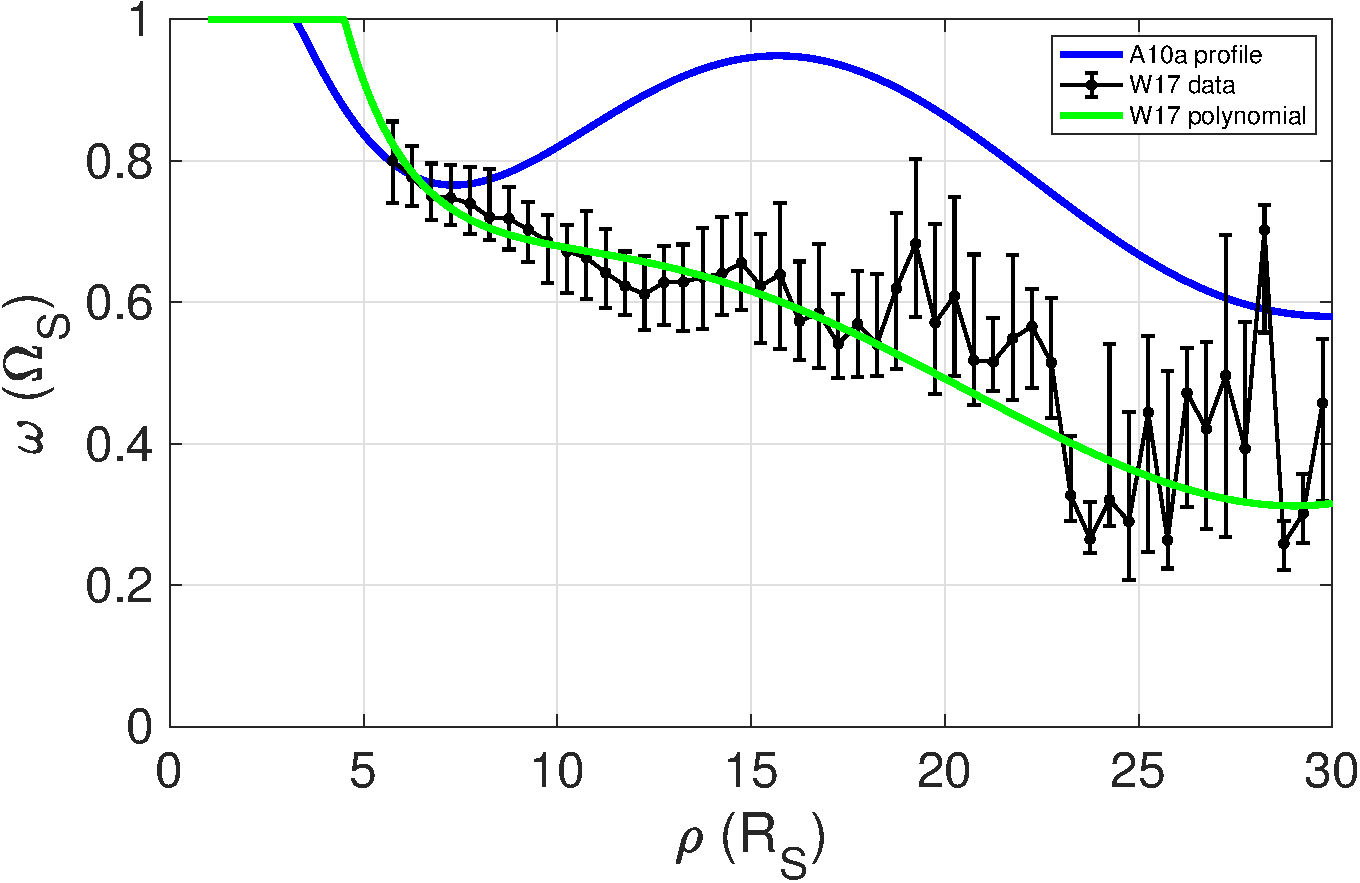
\includegraphics[width=0.8\textwidth]{appendix/omegaprofile.pdf}
\caption[Equatorial profile of plasma angular velocity from \citet{wilson2017}, with best fit polynomial.]{Plasma angular velocity at the equator as a fraction of planetary corotation, as a function of cylindrical radial distance. Black solid circles and error bars show the median and upper/lower quartile values of binned measurements of azimuthal velocity from \citet{wilson2017}, converted to angular velocity as described in the text. The green line shows the fourth-order polynomial fit to these points. The blue line shows the original angular velocity profile used in the \citet{achilleos2010a} model.}
\label{appendix:fig:omegaprofile}
\end{figure}
\citet{alexeev2005,alexeev2006}
In Chapter~\ref{chap:equinox}, we mentioned how we updated the equatorial profile of plasma angular velocity $\omega$ in the UCL/AGA magnetodisc model. The original profile was a sixth-order polynomial fit to azimuthal velocity measurements from studies by \citet{wilson2008} (for $5<\rho<\SI{10}{R_S}$), who used CAPS/IMS data, and \citet{kane2008} (for ${\sim}13<\rho<\SI{35}{R_S}$), who used MIMI/INCA data \citep[more detail in][]{achilleos2010a}. This profile is shown by the blue line in Figure~\ref{appendix:fig:omegaprofile}. To better represent the plasma behaviour particularly in the outer magnetosphere, we updated this profile using more recent azimuthal velocity measurements from the study by \citet{wilson2017}. In that study the authors employed a more comprehensive CAPS data set, and an improved fitting technique, to derive median and upper/lower quartile values for equatorial azimuthal velocity in $\SI{0.5}{R_S}$ width radial bins between 5.5 and $\SI{30}{R_S}$. These values, converted to angular velocities as a fraction of corotation using a planetary rotation rate $\Omega_S = \SI{1.6185e-4}{\radian\per\second}$ ($\SI{10.7833}{\hour}$ period), are shown by the black solid circles and error bars in Figure~\ref{appendix:fig:omegaprofile}. We fit the median values of azimuthal velocity with a fourth-order polynomial, of the form 
%v_\phi = a_1\rho^4 + a_2\rho^3 + a_3\rho^2 + a_4\rho +a_5
\begin{equation} \label{appendix:eq:fourthorderpolyv}
v_\phi = a_0 + a_1\rho + a_2\rho^2 + a_3\rho^3 + a_4\rho^4,
\end{equation}
with each point weighted by the inverse square of the error (assumed to be half of the interquartile range of the bin). With $v_\phi$ in units of $\si{km\per\second}$ and cylindrical radial distance $\rho$ in units of $\si{R_S}$, we found the best fit coefficients as follows:
\begin{align}
& a_0 = 68.5 \\
& a_1 = -13.5 \nonumber \\
& a_2 = 2.22 \nonumber \\
& a_3 = -0.106 \nonumber \\
& a_4 = 0.00158. \nonumber
\end{align}
The resulting angular velocity profile, which was used for the UCL/AGA models in the studies in Chapter~\ref{chap:equinox} and~\ref{chap:LTsectors}, is shown by the green line in Figure~\ref{appendix:fig:omegaprofile}. We assumed that the plasma is in ideal corotation inside $\SI{4.5}{R_S}$, and constant plasma angular velocity beyond $\SI{29}{R_S}$ equal to the value at that point, to ensure a continuous profile. Alternatively, we could have assumed that the angular velocity decreases as $1/\rho^2$ beyond $\SI{29}{R_S}$, such that total angular momentum is conserved; however we found that this had only a very small impact on the resulting equatorial magnetic field profile of the model (less than $\SI{0.1}{nT}$ maximum difference for a $R_\mathrm{D} = \SI{45}{R_S}$ dayside model, at the very outer edge of the magnetosphere) and thus such an approach would not change the conclusions of the studies presented in this thesis.


\section{Cold Ion Temperatures}\label{appendix:sec:temperature}
In Chapter~\ref{chap:LTsectors}, we mentioned how we updated the representation of the cold equatorial ion temperatures used as a boundary condition in the UCL/AGA magnetodisc model. The original profile was based on fourth-order polynomial fits to measurements of the perpendicular and parallel temperatures for hydrogen and water group ions from studies by \citet{wilson2008} (for $5<\rho<\SI{10}{R_S}$) and \citet{mcandrews2009} (for ${\sim}{10}<\rho<\SI{25}{R_S}$), both based on CAPS/IMS data, as described in \citet{achilleos2010b}. These profiles are shown by the black and grey lines in Figure~\ref{appendix:fig:tempprofile}. We updated these profiles using the aforementioned more comprehensive data set from \citet{wilson2017}, shown by the blue and red points in Figure~\ref{appendix:fig:tempprofile}. We used a a fit function of the form
\begin{equation} \label{appendix:eq:fourthorderpolyT}
\log{T} = a_0+a_1\rho + a_2\rho^2 + a_3\rho^3 + a_4\rho^4
\end{equation}
with $T$ in units of $\si{eV}$ and cylindrical radial distance $\rho$ in units of $\si{R_S}$, again weighting each point by the inverse square of the error (assumed to be half the interquartile range of each bin). The coefficients of the best fit polynomials for each ion species are given in Table~\ref{appendix:tab:wilsonTpolys}.
\begin{table}
\caption{Coefficients of fourth-order polynomial fits to the logarithm of the parallel and perpendicular temperatures for water group ($W^+$) and hydrogen ($H^+$) ions from \citet{wilson2017}.}\label{appendix:tab:wilsonTpolys}
\centering
\begin{tabular}{c | c c | c c} 
\hline
Moment 		& \multicolumn{2}{c |}{$T_\mathrm{perpendicular}$} 								& 	\multicolumn{2}{c}{$T_\mathrm{parallel}$} 	 \\
Ion Species	&	$H^+$																&	$W^+$ 				&	$H^+$																		&	$W^+$ \\
\hline
$a_0$			&	-0.687																&	1.29						&	0.461																		&	0.221\\
$a_1$			&	0.530																&	0.201					& 	0.114																		&	0.352 \\
$a_2$			&	-0.0500															&	-0.0168				& -0.00770																	&	-0.0229\\
$a_3$			& 0.00208															&	\num{6.67e-4}	& \num{3.98e-4}															&	\num{7.35e-4}\\
$a_4$			& \num{-3.02e-5}												&	\num{-9.31e-6}	& \num{-7.24e-6}														&\num{-9.15e-6}\\
\hline
\end{tabular}
\end{table}
We found that this modification did not significantly affect the overall resulting magnetic field profile of the magnetodisc models, in general causing only a slight increase in magnetic field strength in the inner magnetosphere, and slight decrease in the outer magnetosphere, with a maximum difference under $\SI{1}{nT}$ for a typical dayside model. However this modification did improve model estimates of the cold plasma pressure, reducing the values in the outer magnetosphere such that they showed better agreement with recent observations from \citet{sergis2017}, also based on CAPS data.

\begin{figure}
\centering
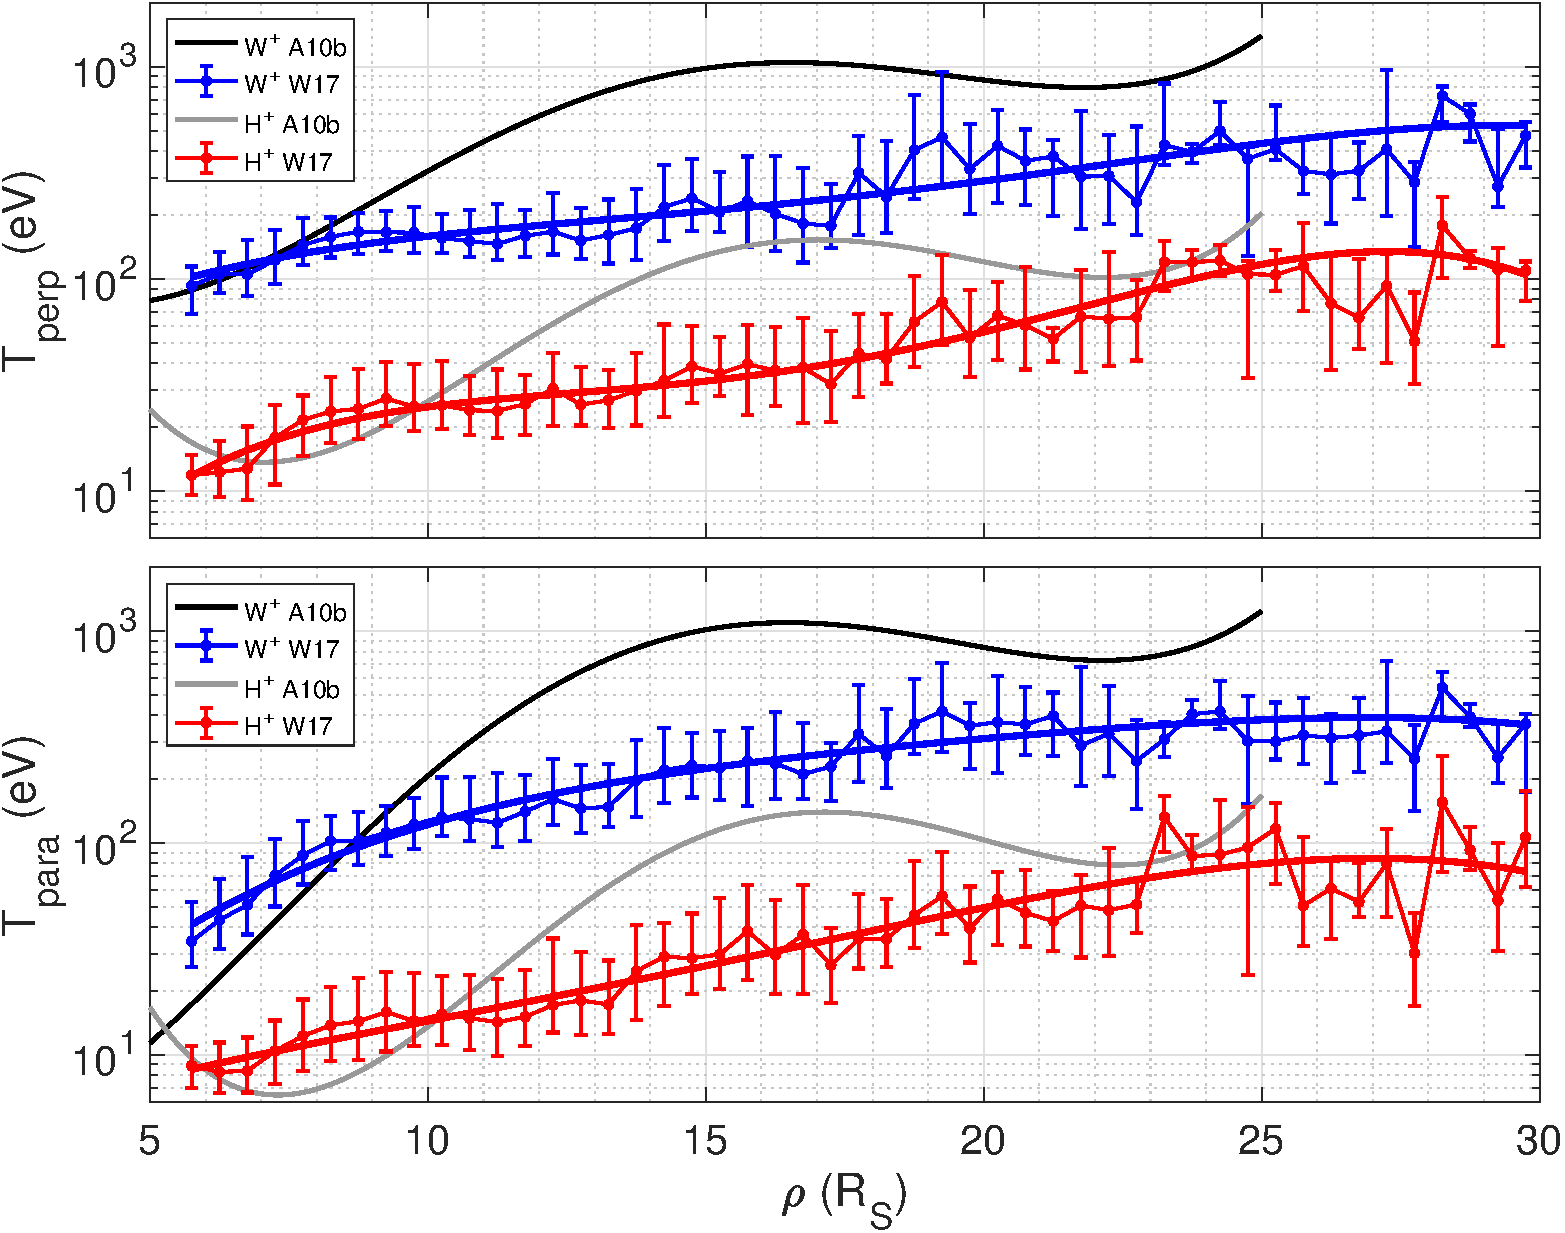
\includegraphics[width=0.8\textwidth]{appendix/tempprofile.pdf}
\caption[Equatorial profiles of temperature moments from \citet{wilson2017}, with best fit polynomials.]{Perpendicular (top panel) and parallel (bottom panel) temperature moments at the equator for water group and hydrogen ions. In each panel, blue and red solid circles with error bars show the median and upper/lower quartiles values of binned measurements for the water group and hydrogen ions respectively, from \citet{wilson2017} CAPS obervations. Solid blue and red lines show the corresponding fourth-order polynomial fits to those points. Black and grey solid lines in each panel show the original profiles for each species used in the \citet{achilleos2010b} model.}
\label{appendix:fig:tempprofile}
\end{figure}
%\chapter{Another Appendix About Things}
%\label{appendixlabel2}
%(things)

%\chapter{Colophon}
%\label{appendixlabel3}
%\textit{This is a description of the tools you used to make your thesis. It helps people make future documents, reminds you, and looks good.}

%\textit{(example)} This document was set in the Times Roman typeface using \LaTeX\ and Bib\TeX , composed with a text editor. 
 % description of document, e.g. type faces, TeX used, TeXmaker, packages and things used for figures. Like a computational details section.
% e.g. http://tex.stackexchange.com/questions/63468/what-is-best-way-to-mention-that-a-document-has-been-typeset-with-tex#63503

% Side note:
%http://tex.stackexchange.com/questions/1319/showcase-of-beautiful-typography-done-in-tex-friends 
% You could separate these out into different files if you have
%  particularly large appendices.

% This line manually adds the Bibliography to the table of contents.
% The fact that \include is the last thing before this ensures that it
% is on a clear page, and adding it like this means that it doesn't
% get a chapter or appendix number.
%\addcontentsline{toc}{chapter}{Bibliography}

% Actually generates your bibliography.
\bibliography{main}

% All done. \o/
\end{document}
